\documentclass[../main.tex]{subfiles}
\begin{document}
\chapter{Resultados}
A continuación se reportan los resultados obtenidos con la metodología descrita en el capítulo anterior.
\section{Muestras Sintetizadas} \label{sec:sintesis}
Se sintetizaron un total de 8 muestras de 1g de cada ortoferrita. Una muestra de cada una fue reservada para realizar un análisis termogravimétrico. A través de éste, se determinó la temperatura mínima de calcinación para ambas ortoferritas, como se reporta en la sección \ref{sec:TGA}.

Con estas temperaturas en mente, 600\gradoC{} para el \neod{} y 700\gradoC{} para el \sama{}, se calcinaron el resto de muestras, 4 muestras de \neod{} se calcinaron a 600\gradoC{}, para las otras 3 se aumentó la temperatura 100\gradoC{} por cada una, es decir, se calcinaron a 700, 800 y 900\gradoC{} respectivamente.

Por otro lado, para el \sama{} se calcinaron 4 muestras a 700\gradoC{}, aumentando la temperatura de la misma forma que en el caso del \neod{} para las otras 3, es decir, se calcinaron a 800, 900 y 1000\gradoC{} respectivamente.

Se obtuvieron polvos de color café rojizo con apariencia porosa, como se muestra en la figura \ref{fig:resfotomuestra}.
\begin{figure}[H]
    \centering
    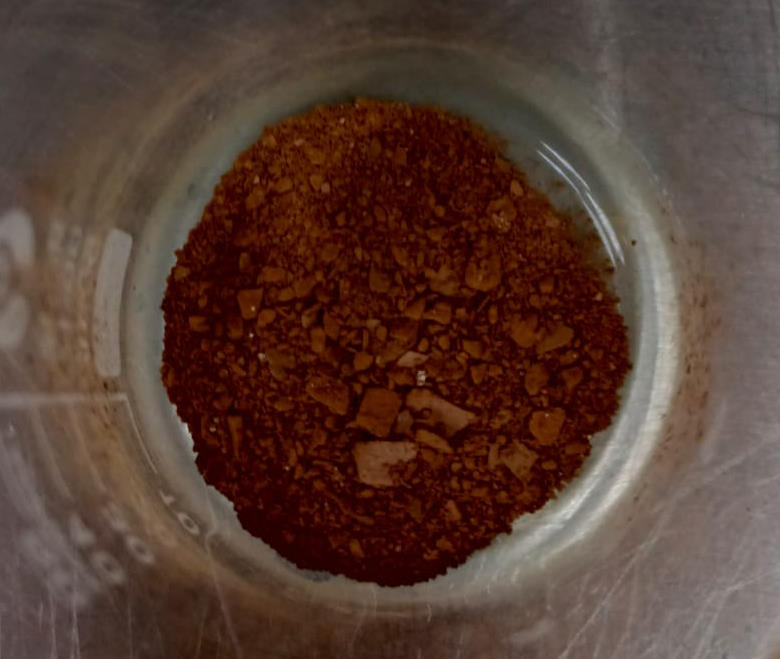
\includegraphics[width=0.7\textwidth]{fig/muestraSmFeO3900.jpeg}
    \caption{Muestra de \sama{} calcinada a 900\gradoC.}
    \label{fig:resfotomuestra}
\end{figure}
\section{Caracterización estructural y morfológica}
En esta sección se reportan los resultados obtenidos a través de las técnicas descritas en el capítulo \ref{cap:metodologia}.
\subsection{Análisis Termogravimétrico} \label{sec:TGA}
Se realizó un análisis termogravimétrico a ambas ortoferritas, lo cual dió como resultado las siguientes curvas de masa contra temperatura:
\begin{figure}[H]
    \centering
    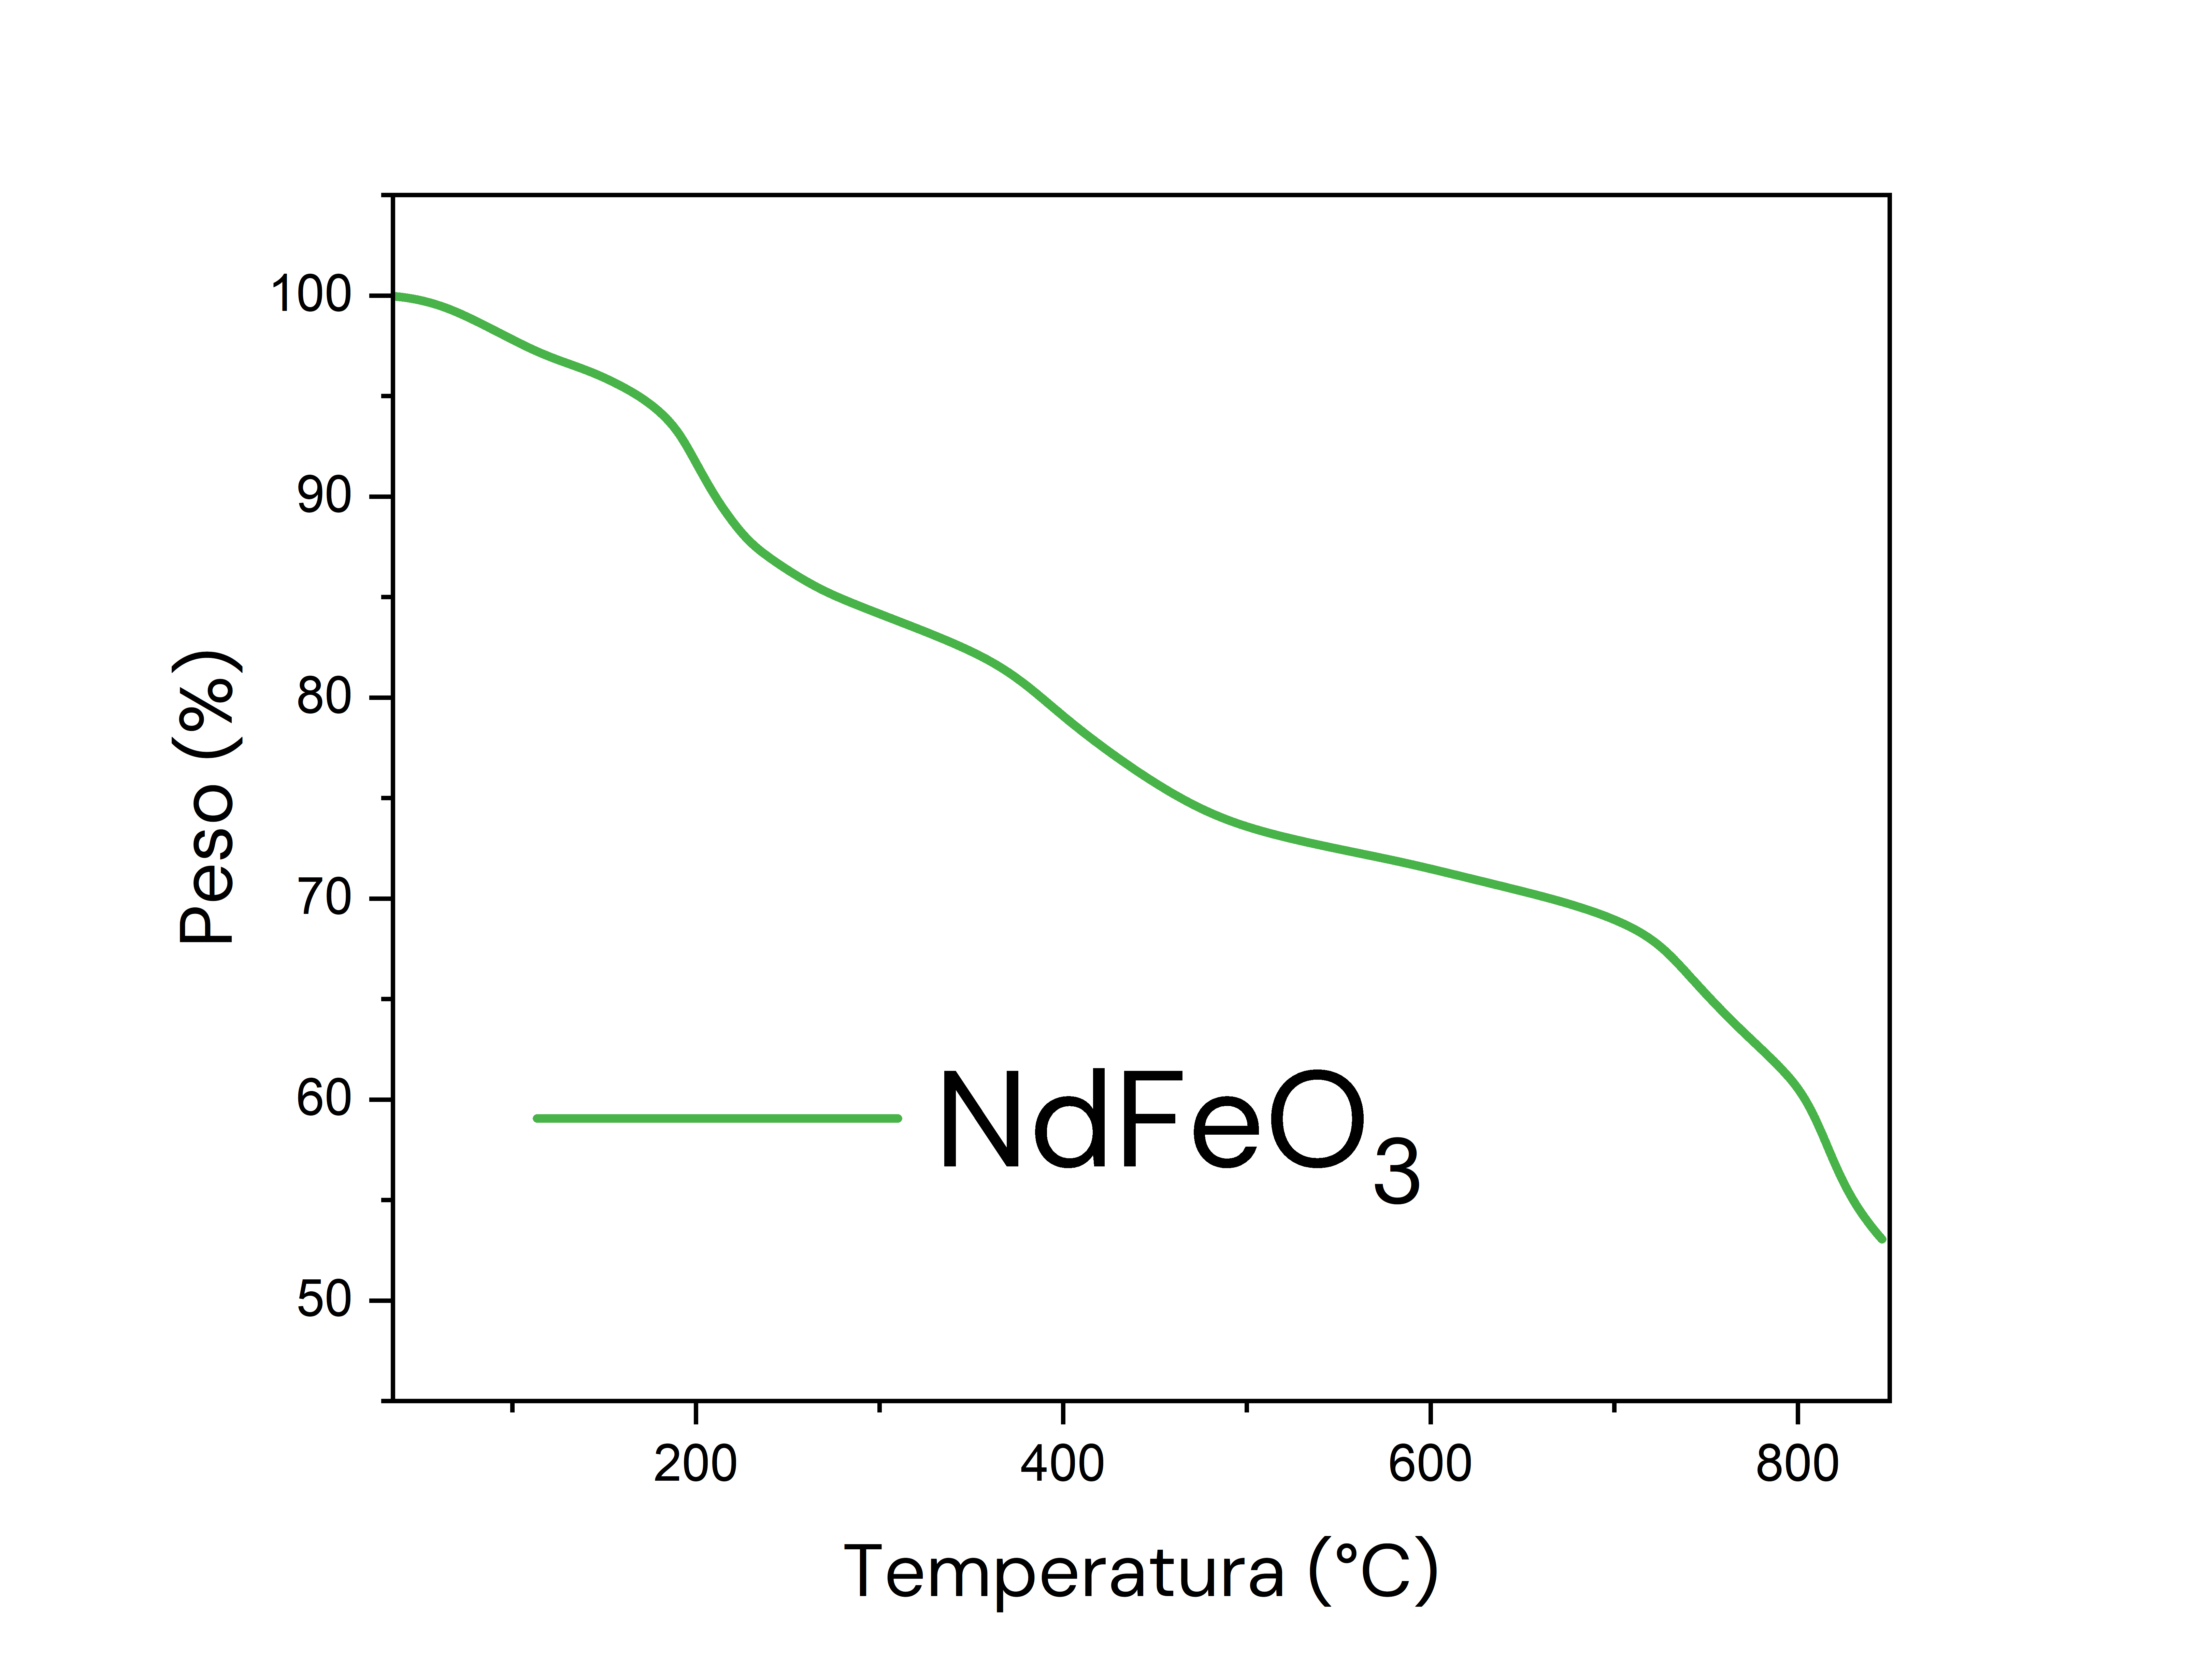
\includegraphics[width=0.4\textwidth]{fig/TGA-NdFeO3.png}
    \quad
    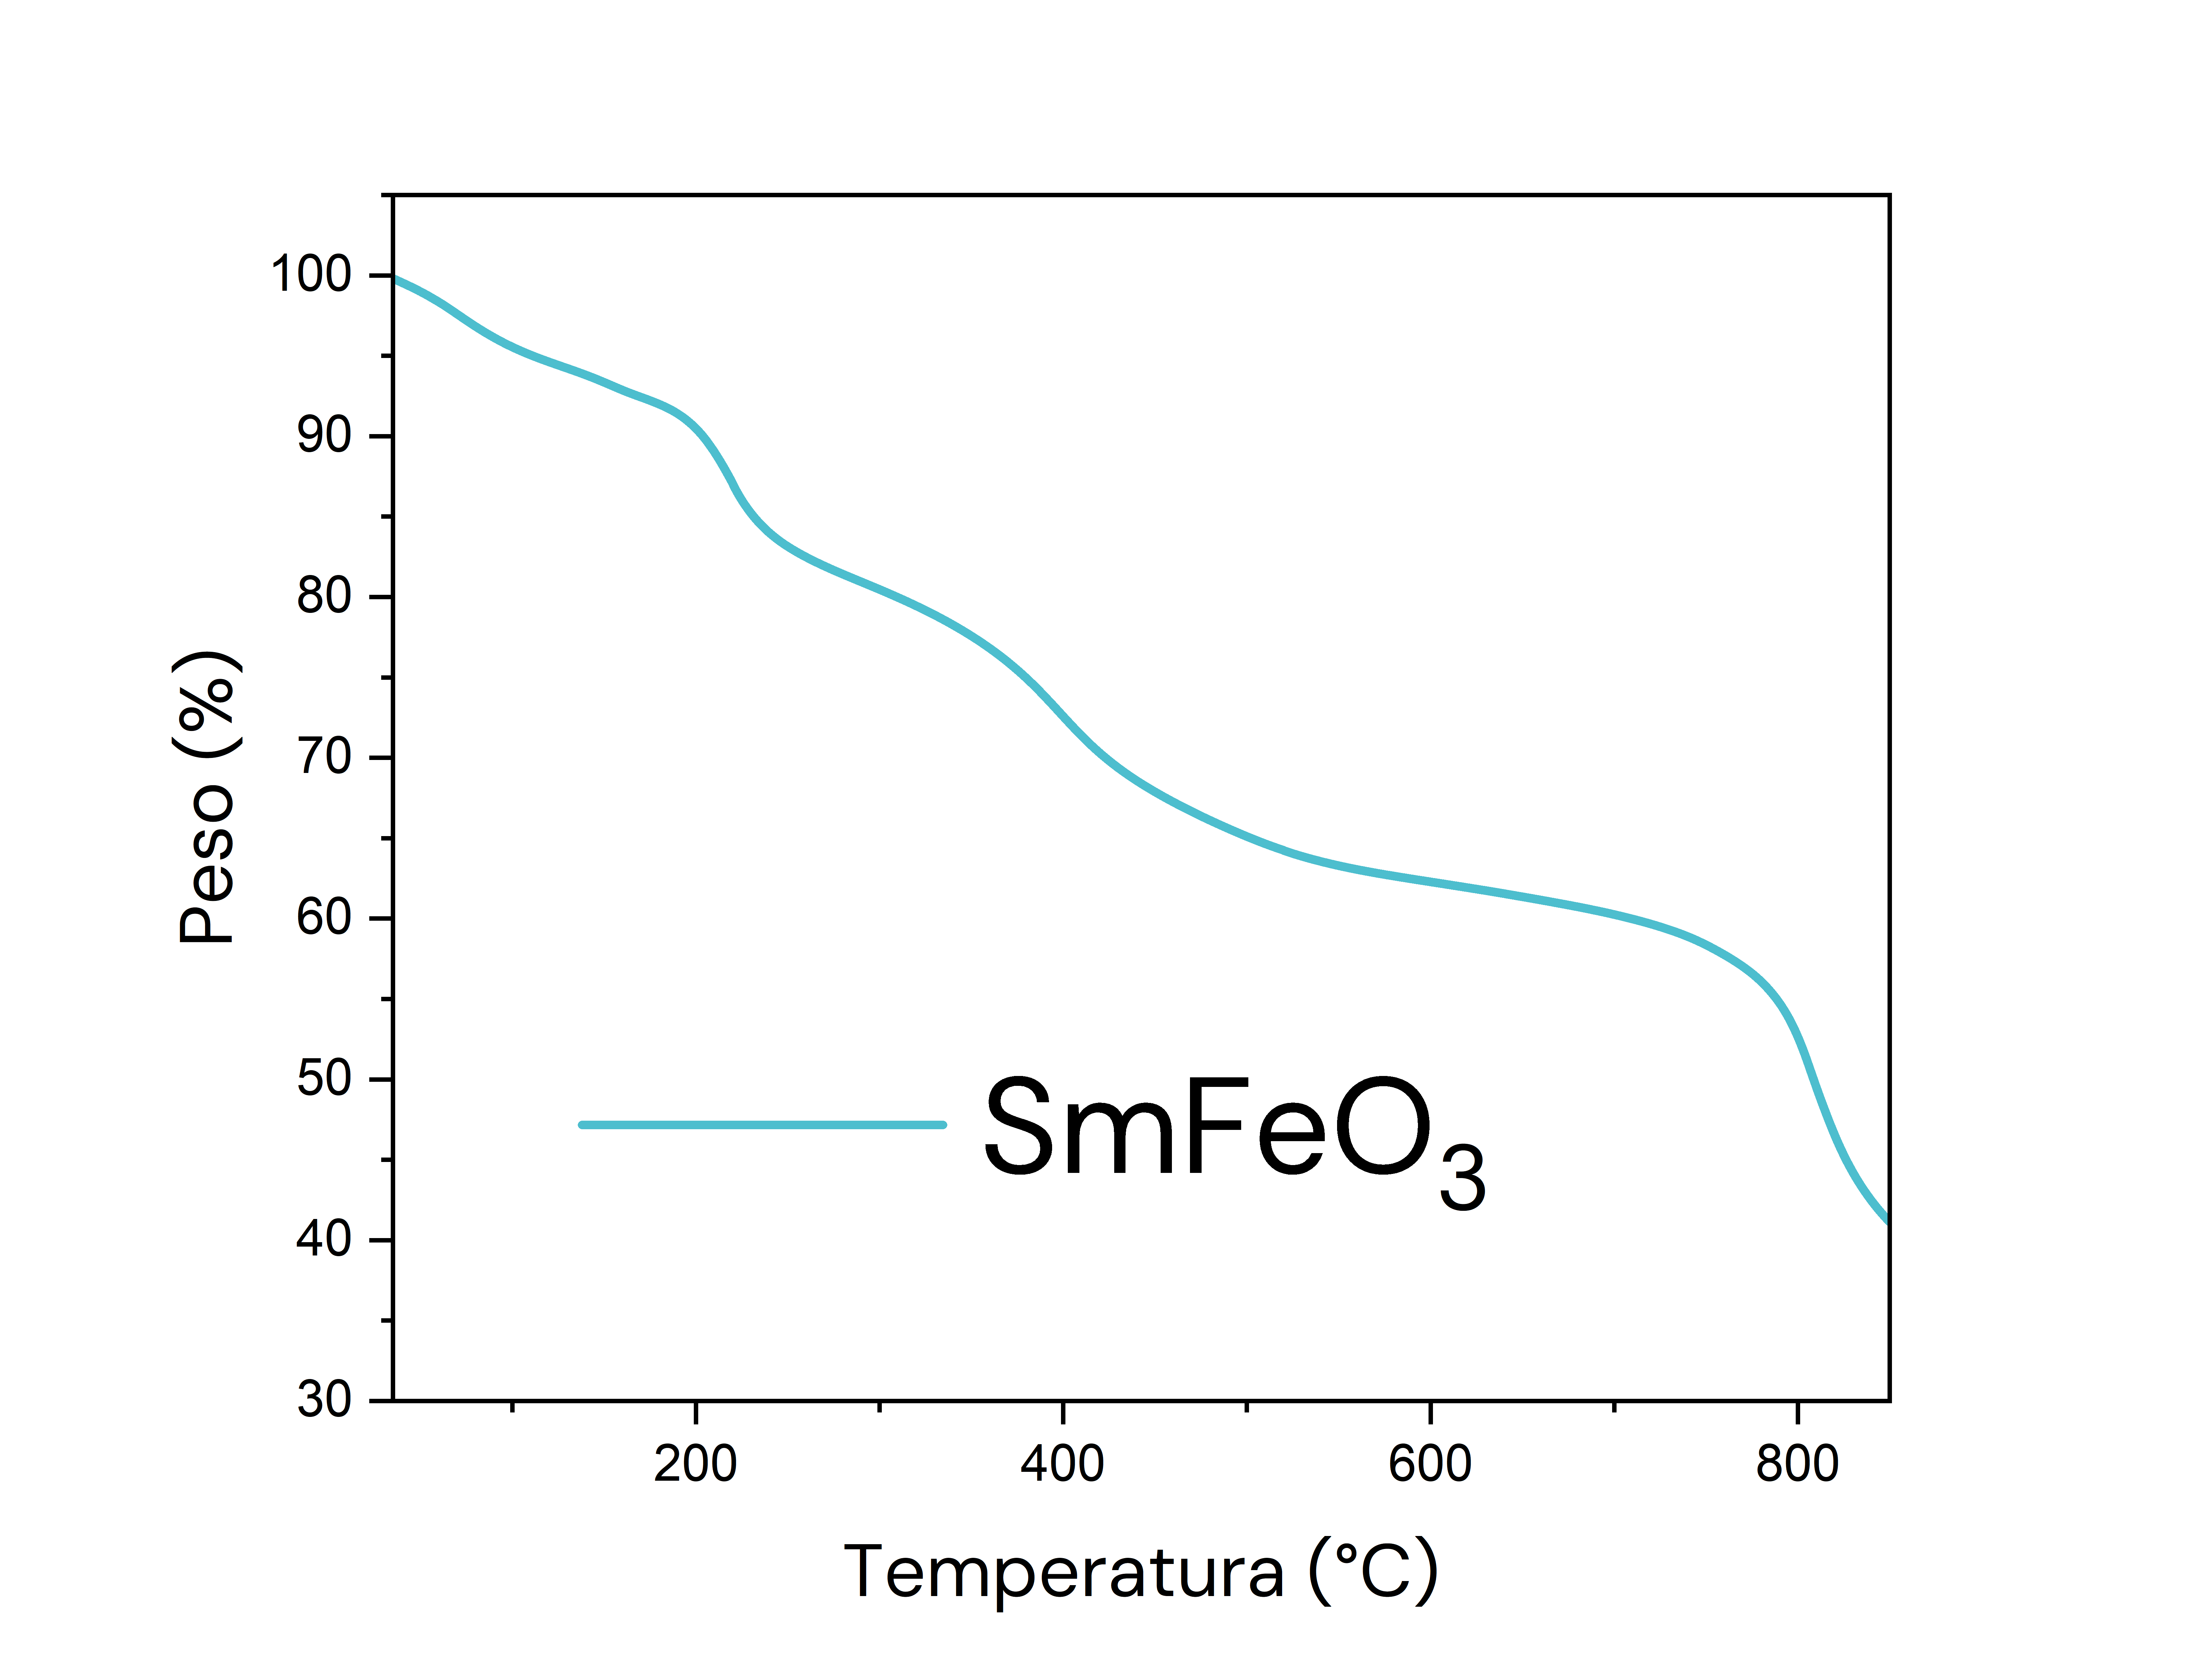
\includegraphics[width=0.4\textwidth]{fig/TGA-SmFeO3.png}
    \caption{Análisis termogravimétrico de las ortoferritas. a) \neod{}, b) \sama{}}
    \label{fig:TGAres}
\end{figure}
Se obtuvo la derivada de la masa respecto a la temperatura:
\begin{figure}[H]
    \centering
    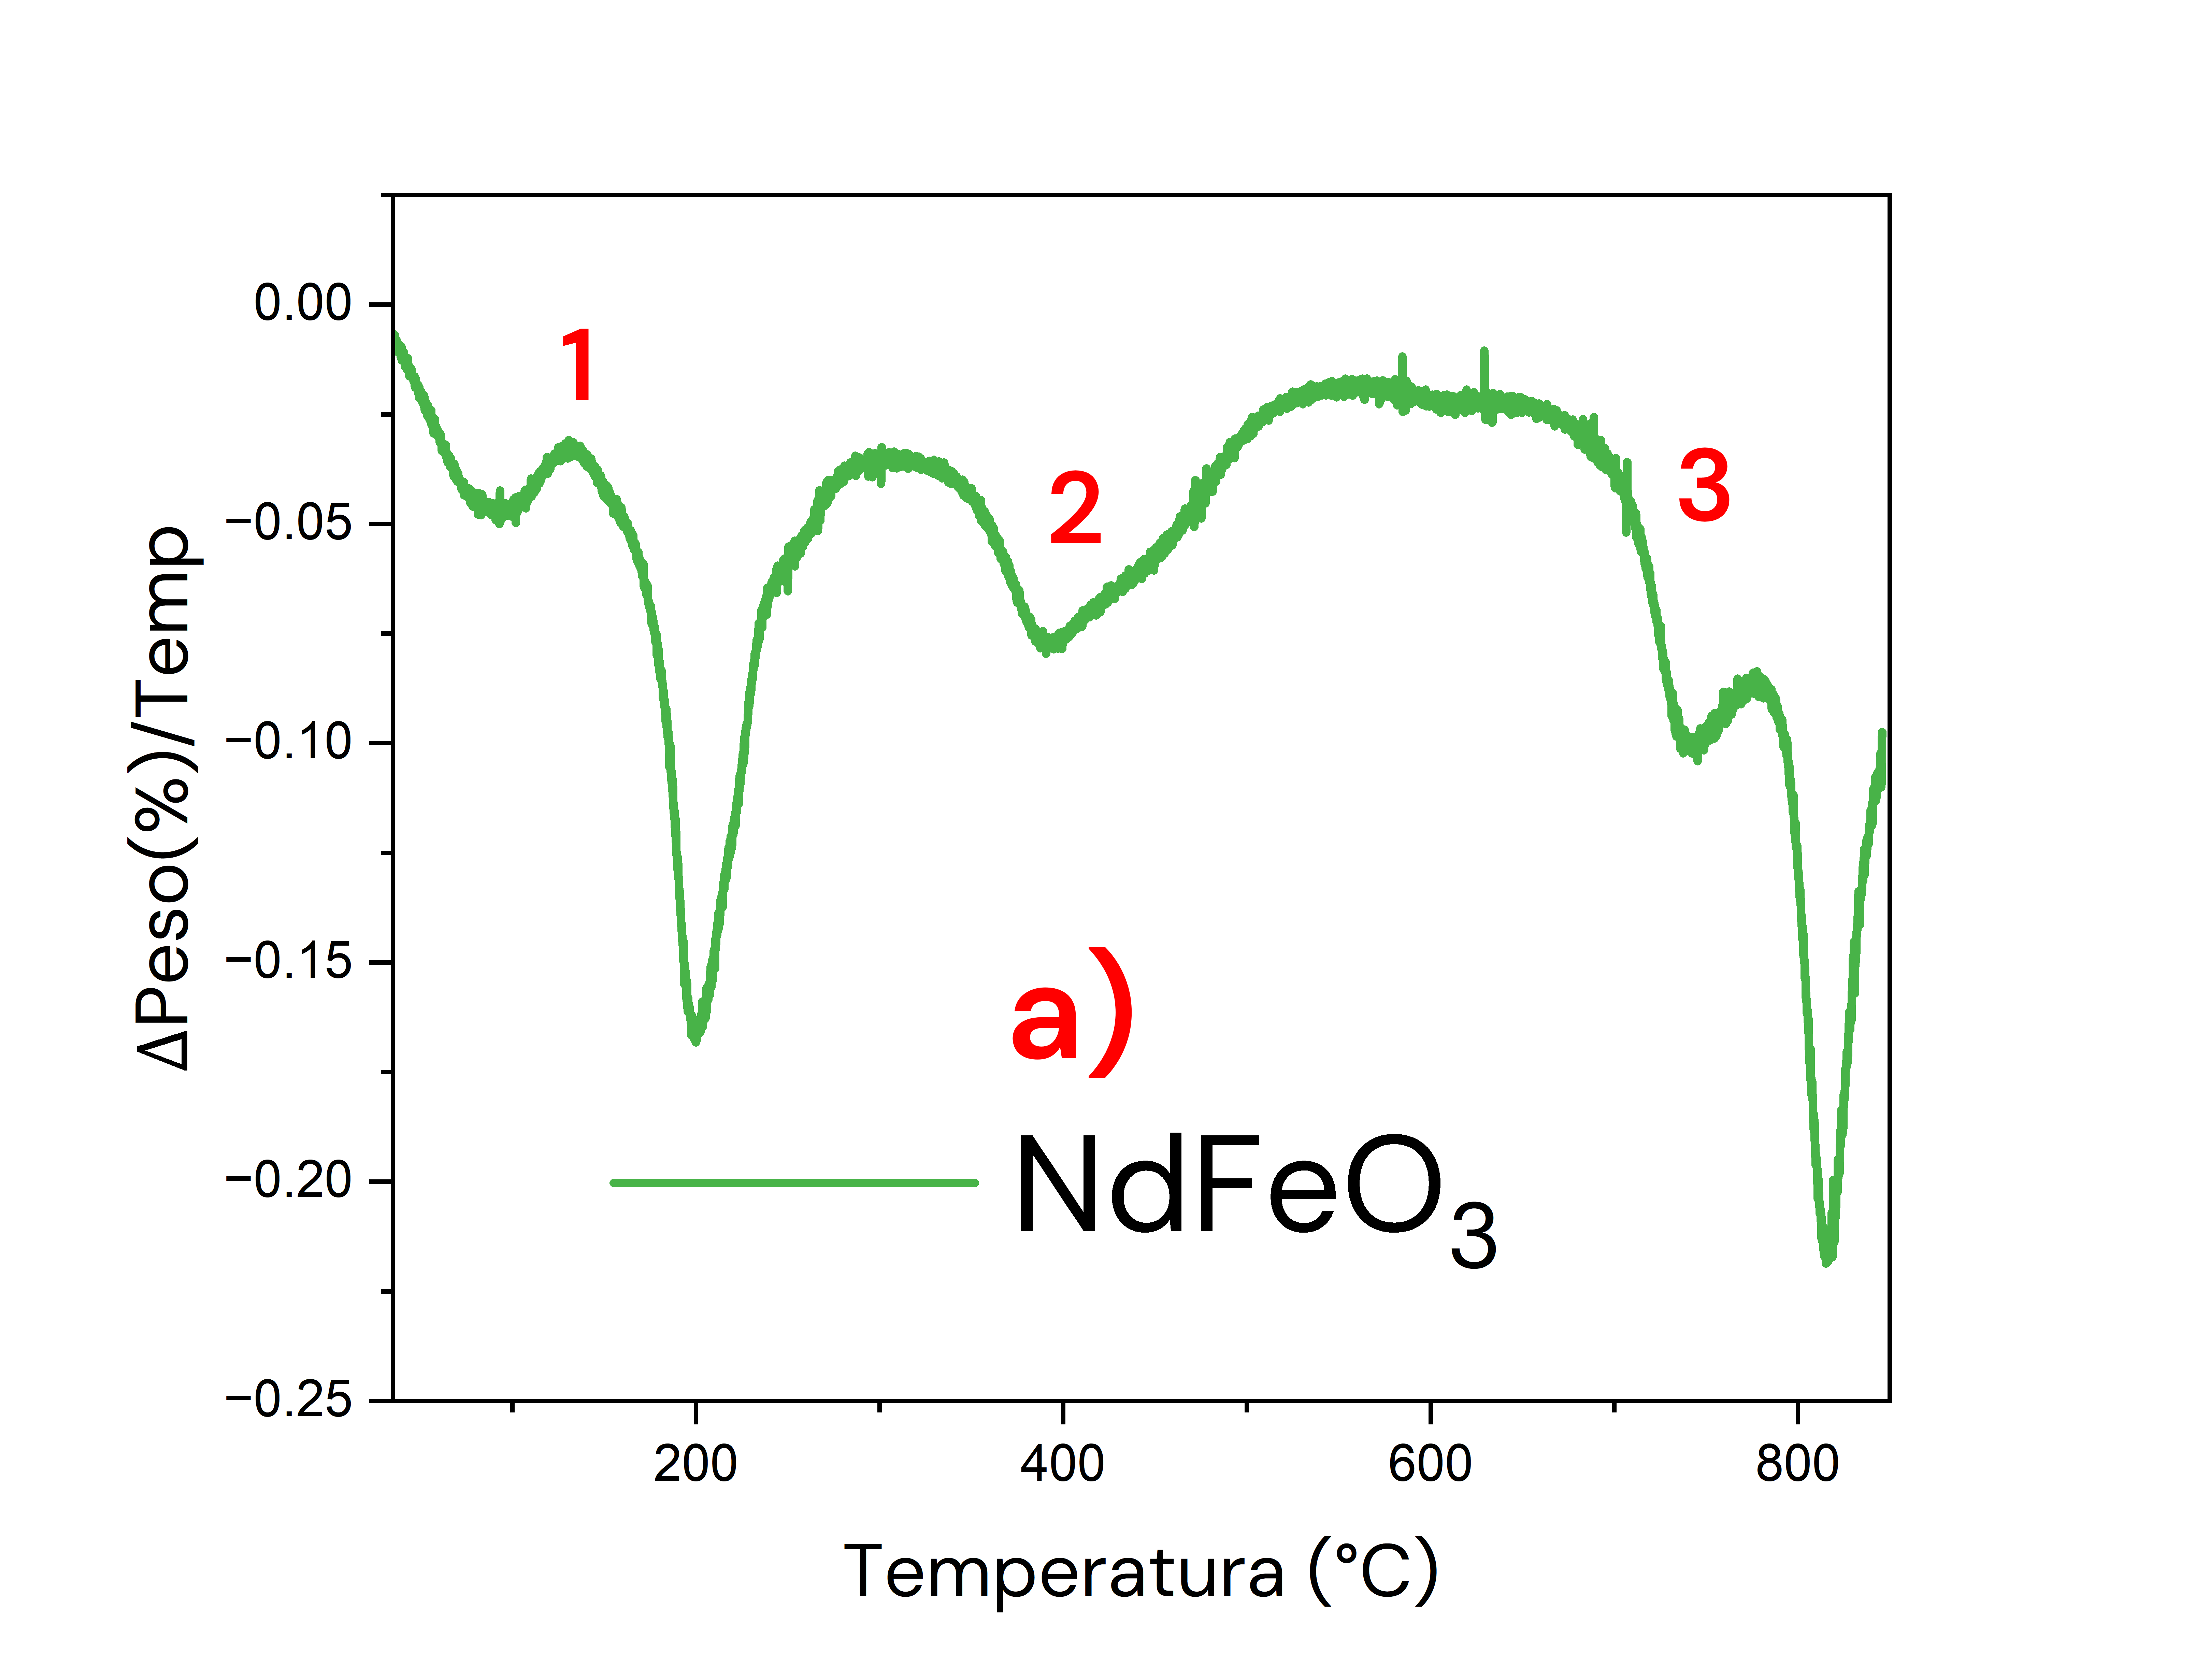
\includegraphics[width=0.4\textwidth]{fig/TGA-derNdFeO3.png}
    \quad
    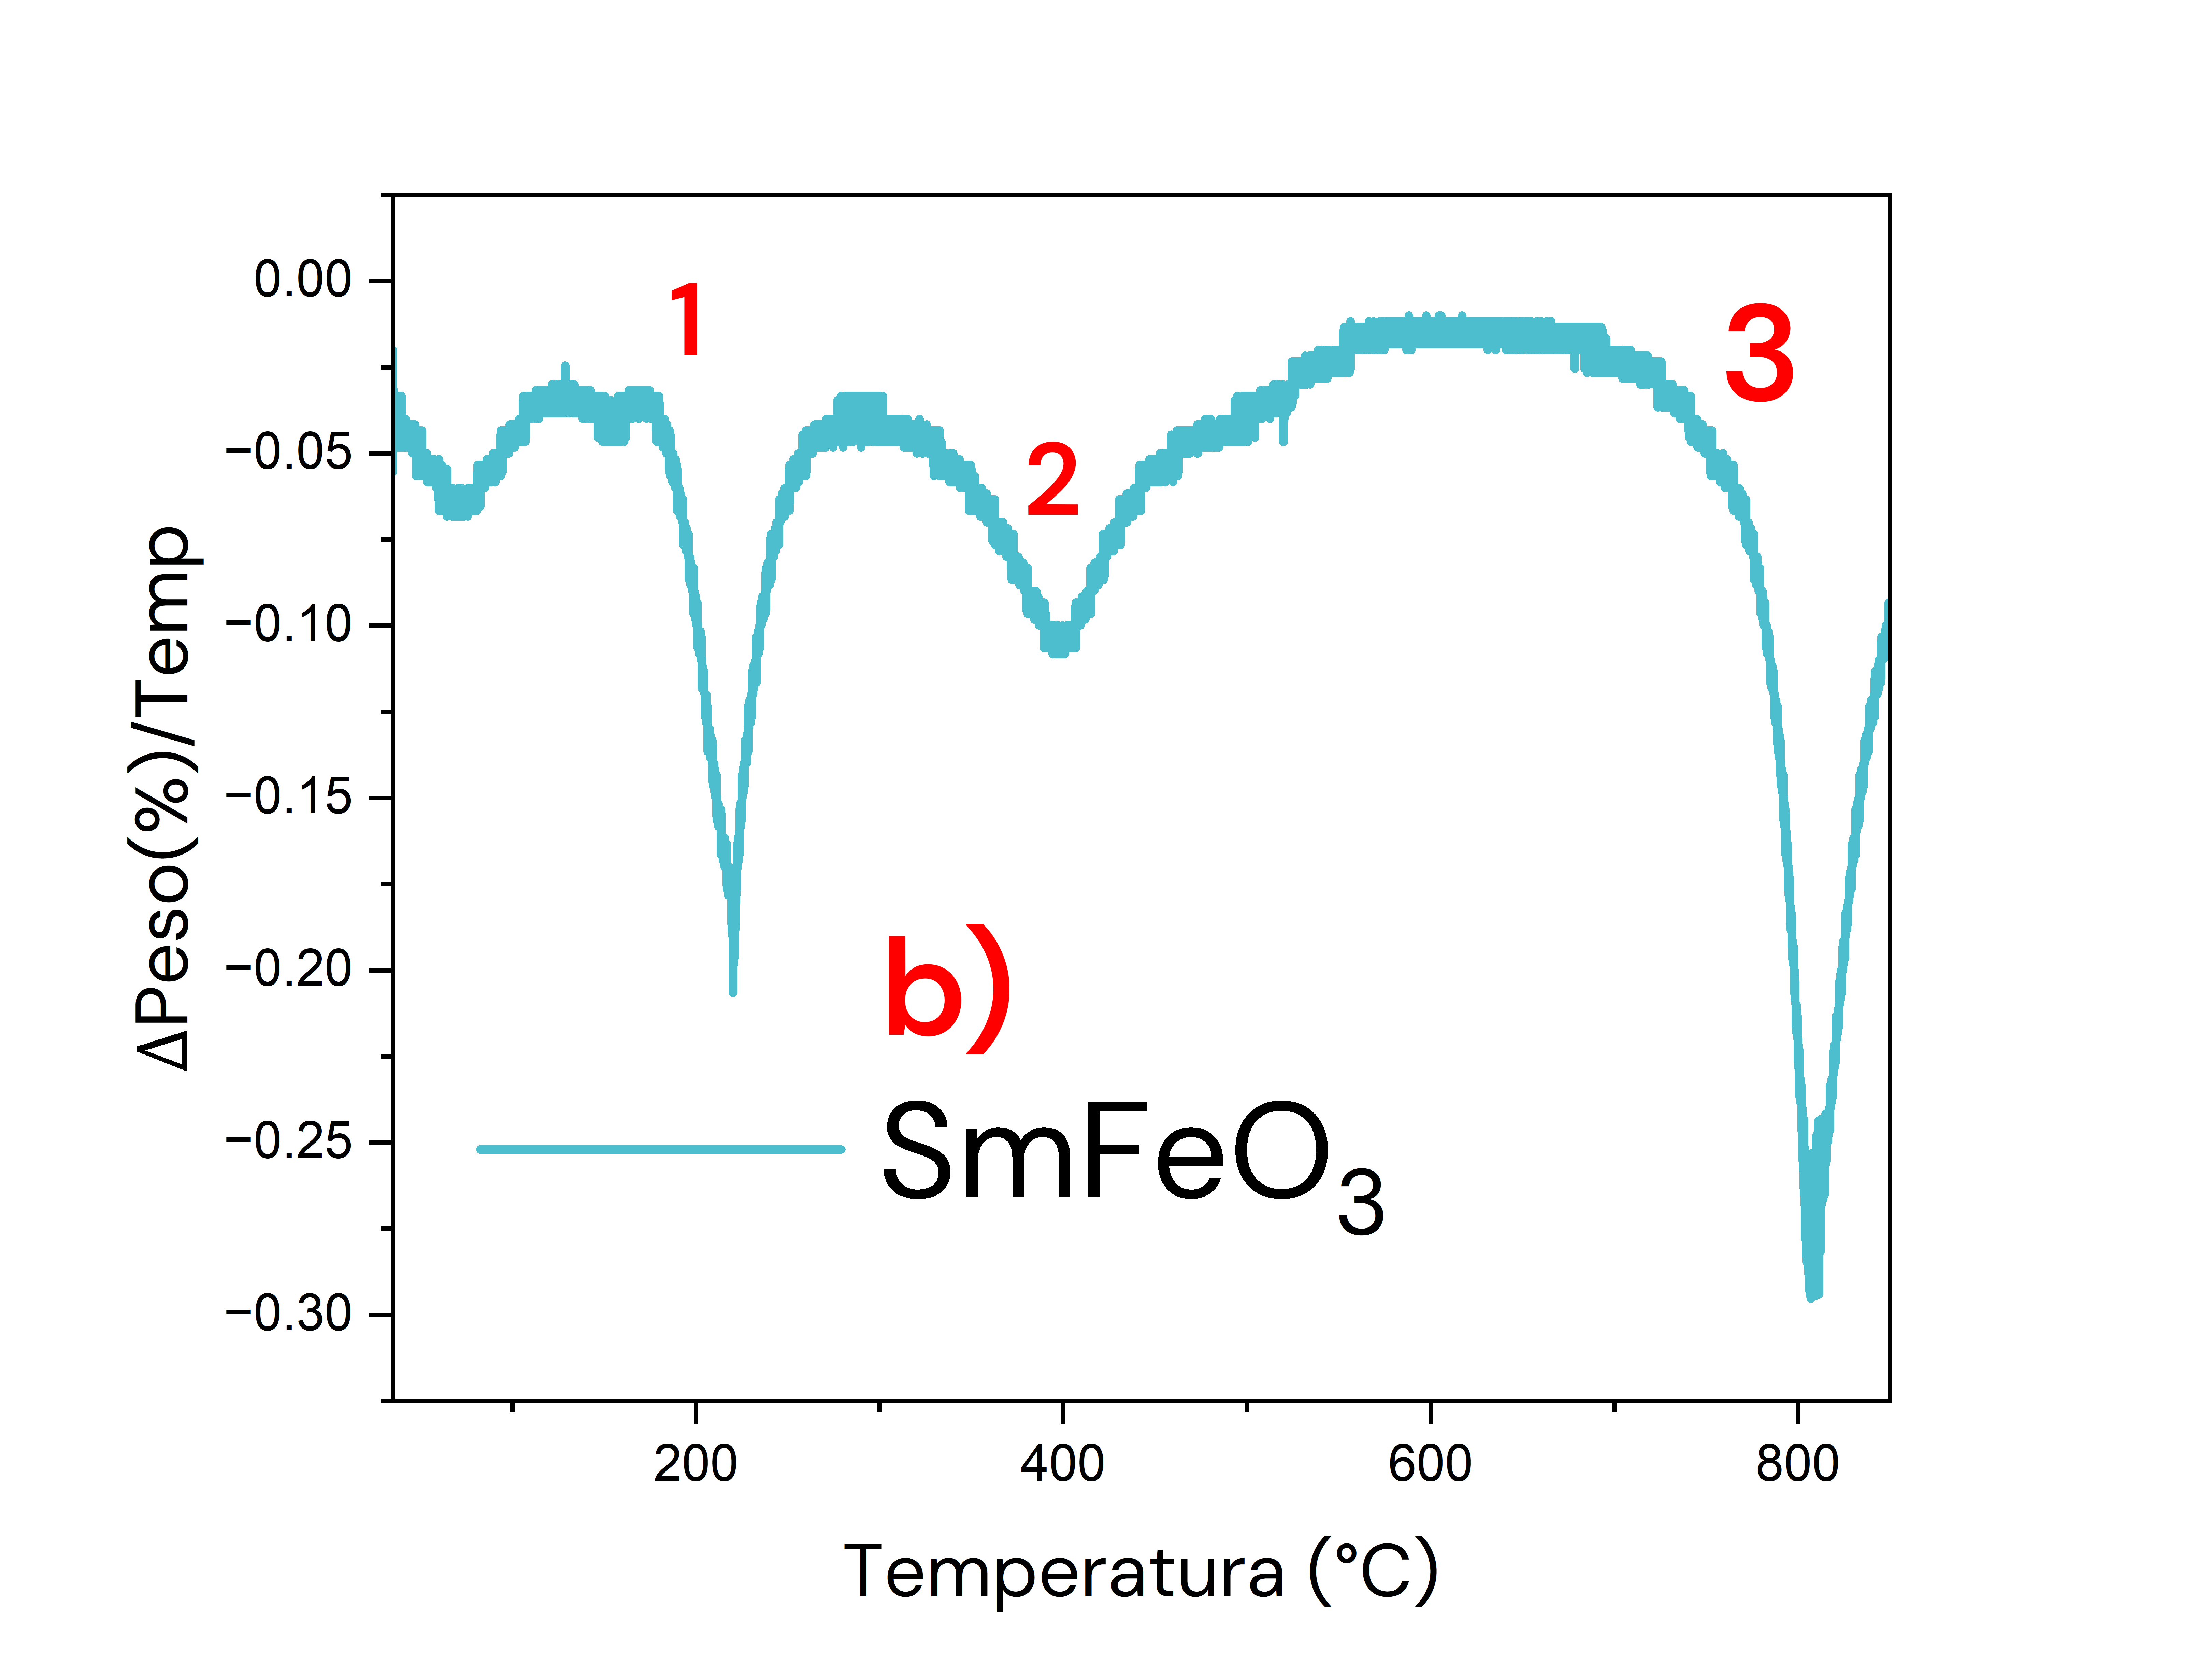
\includegraphics[width=0.4\textwidth]{fig/TGA-derSmFeO3.png}
    \caption{Derivada de la masa respecto a la temperatura para ambas ferritas. a) \neod{}, b) \sama{}}
    \label{fig:derTGAres}
\end{figure}
Se pueden observar 3 regiones distintas donde ocurren cambios térmicos en la muestra:
\begin{table}[H]
    \centering
    \begin{tabular}{|c|c|}
        \hline
        Zona & Temperatura\\
        & aproximada\\\hline\hline
        1&100-200\gradoC{}\\
        \hline
        2&300-500\gradoC\\\hline
        3&>700\gradoC\\
        \hline
    \end{tabular}
    \caption{Regiones donde cambia el comportamiento de la masa respecto a la temperatura para ambas muestras.}
    \label{tabla:TGAtabla}
\end{table}
La región 1 coincide con las temperaturas a la que el agua se evapora y se combustiona la fase orgánica en la muestra.

Por otra parte, se piensa que en la región 2 comienza la cristalización de las ortoferritas, mientras que en la región 3 ocurre un crecimiento de los cristales, de acuerdo con las observaciones que se discutirán en la sección \ref{sec:resrietlveld}.
\subsection{Microscopía electrónica de barrido}
Se estudió la morfología de las partículas sintetizadas a través de esta técnica, dando como resultado imágenes como las que se muestran en las figuras \ref{fig:resSEM900}-\ref{fig:resSEMsonicada4}.
\begin{figure}[H]
    \centering
    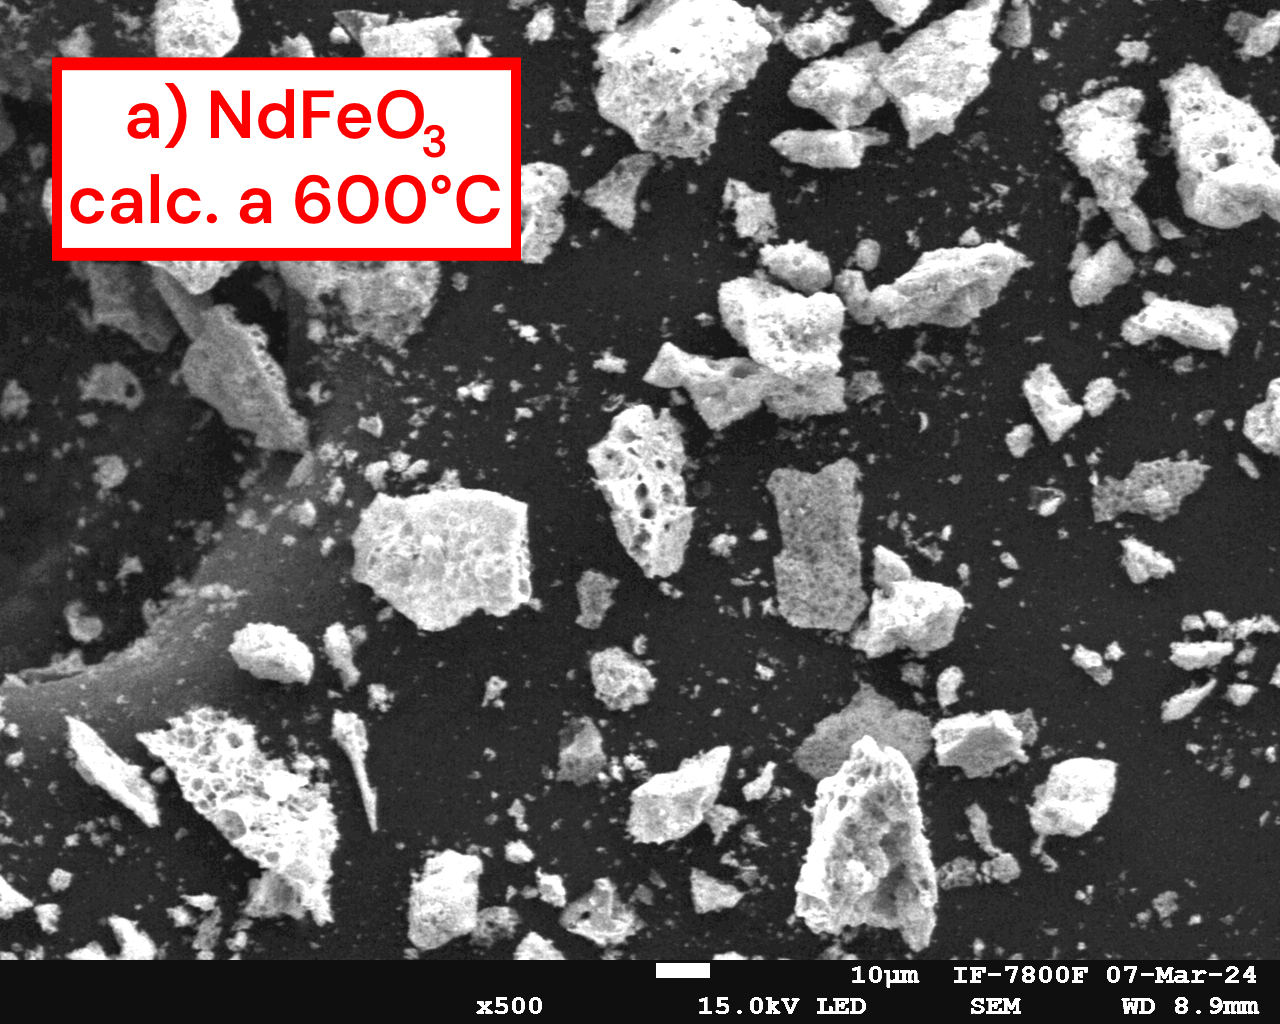
\includegraphics[width=0.45\textwidth]{fig/semneod600.png}
    \quad
    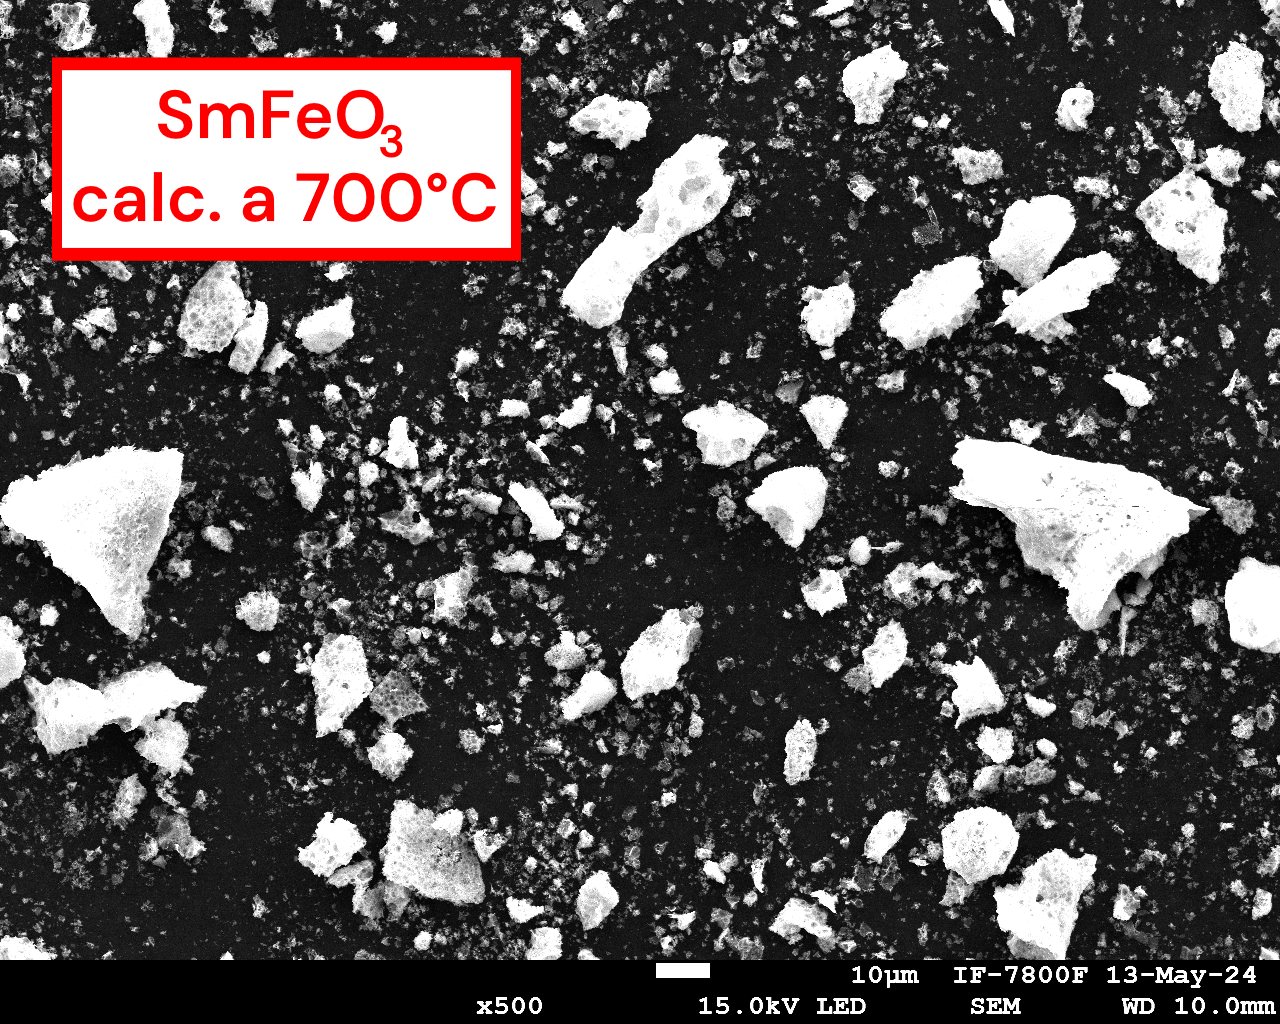
\includegraphics[width=0.45\textwidth]{fig/semsama700.png}
    \caption{Imágenes obtenidas a través de SEM para las muestras sin sonicar. Muestra de a) \neod{} calcinada a 600\gradoC{}, b) \sama{} calcinada a 700\gradoC{}. Amplificación $\times500$}
    \label{fig:resSEMsinsonicar}
\end{figure}
\begin{figure}[H]
    \centering
    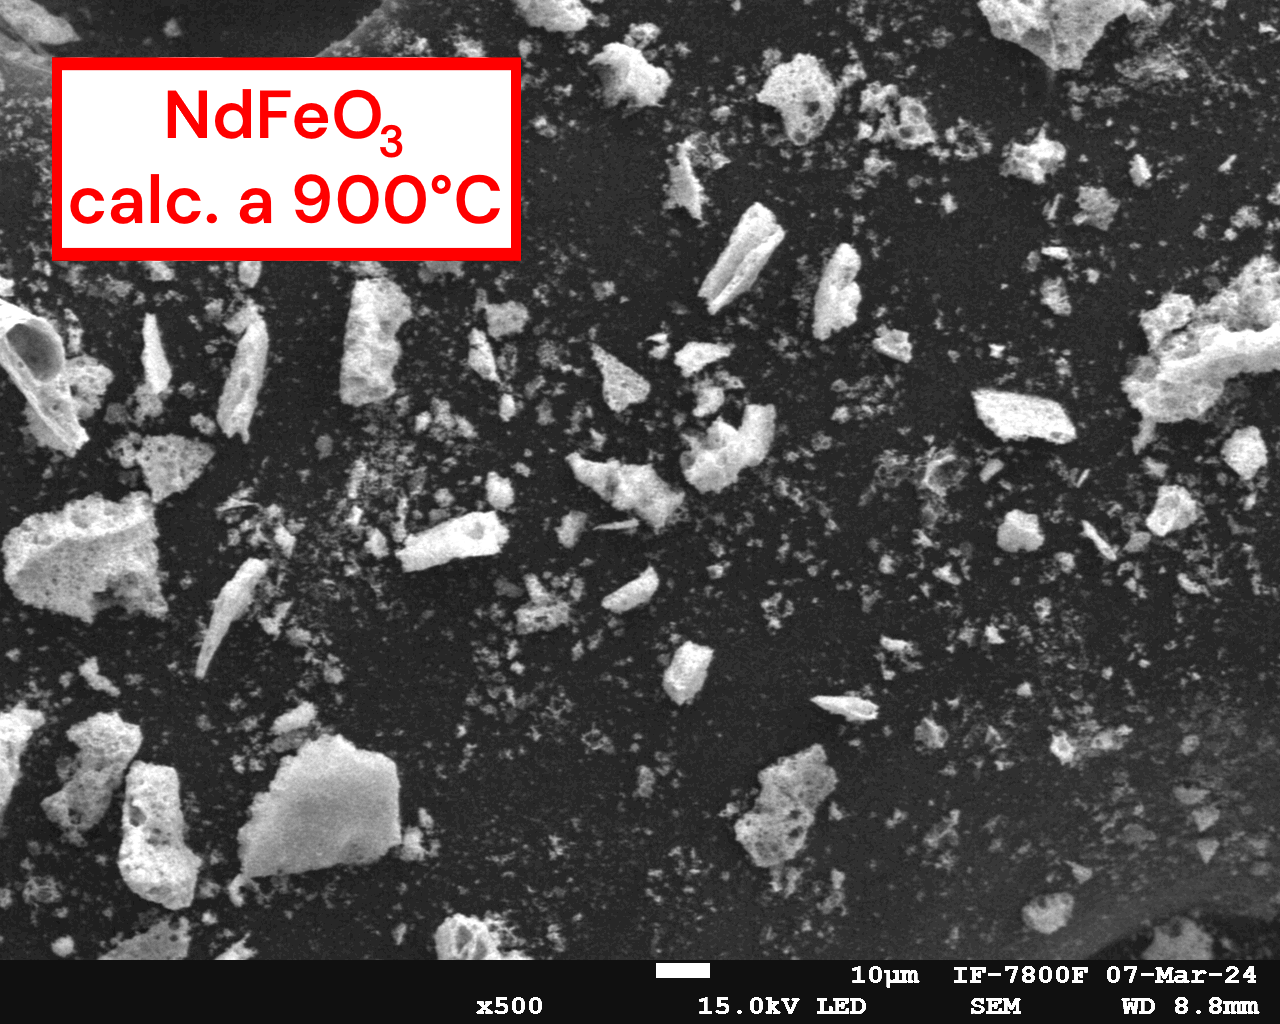
\includegraphics[width=0.45\textwidth]{fig/semneod900.png}
    \quad
    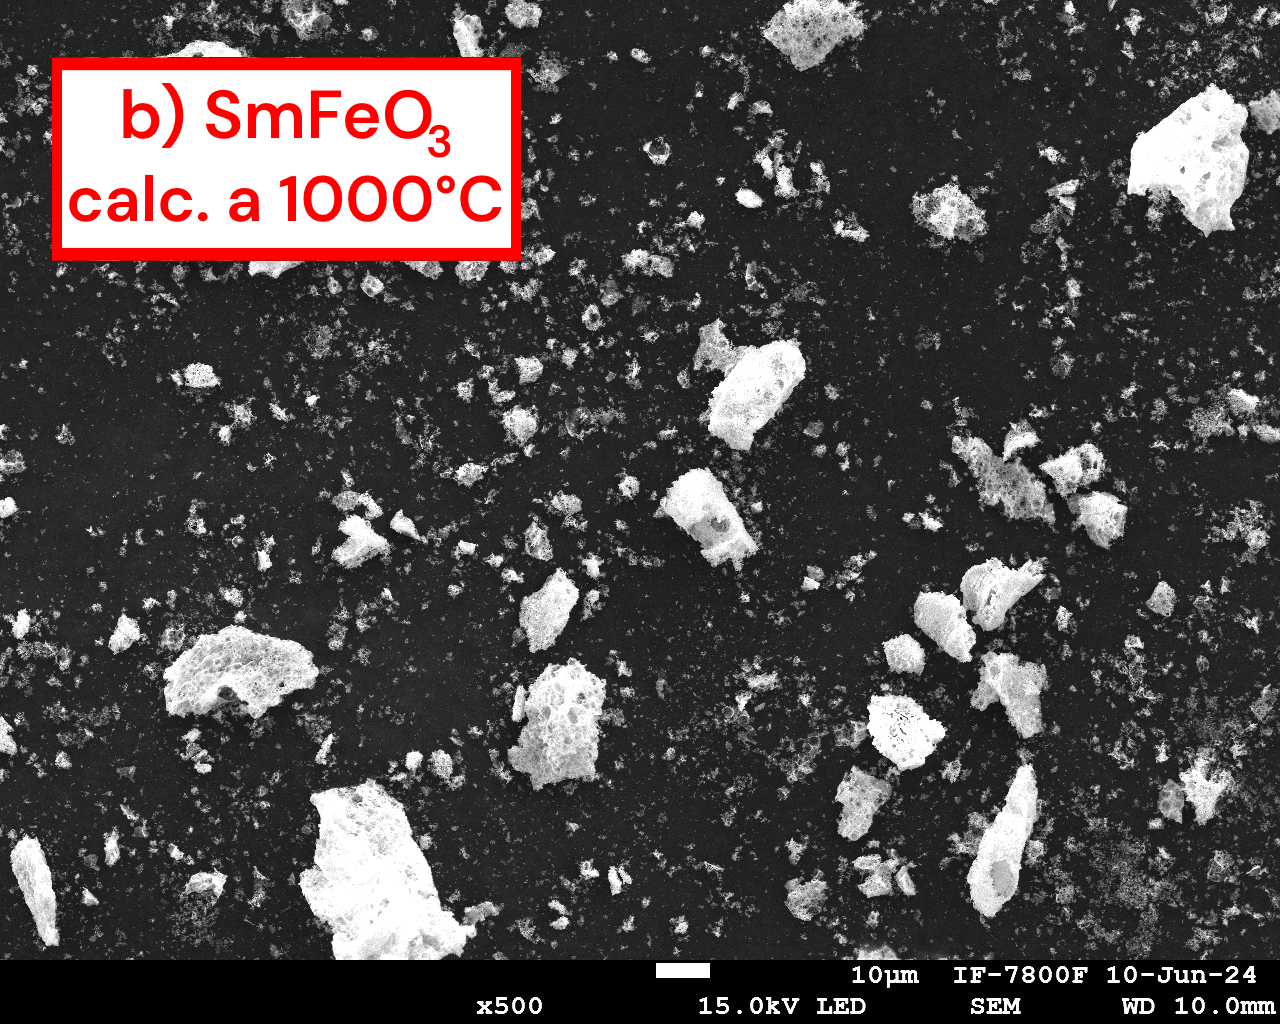
\includegraphics[width=0.45\textwidth]{fig/semsama1000.png}
    \caption{Imágenes obtenidas a través de SEM para las muestras sin sonicar. Muestra de a) \neod{} calcinada a 900\gradoC{}, b) \sama{} calcinada a 1000\gradoC{}. Amplificación $\times500$}
    \label{fig:resSEM900}
\end{figure}
\begin{figure}[H]
    \centering
    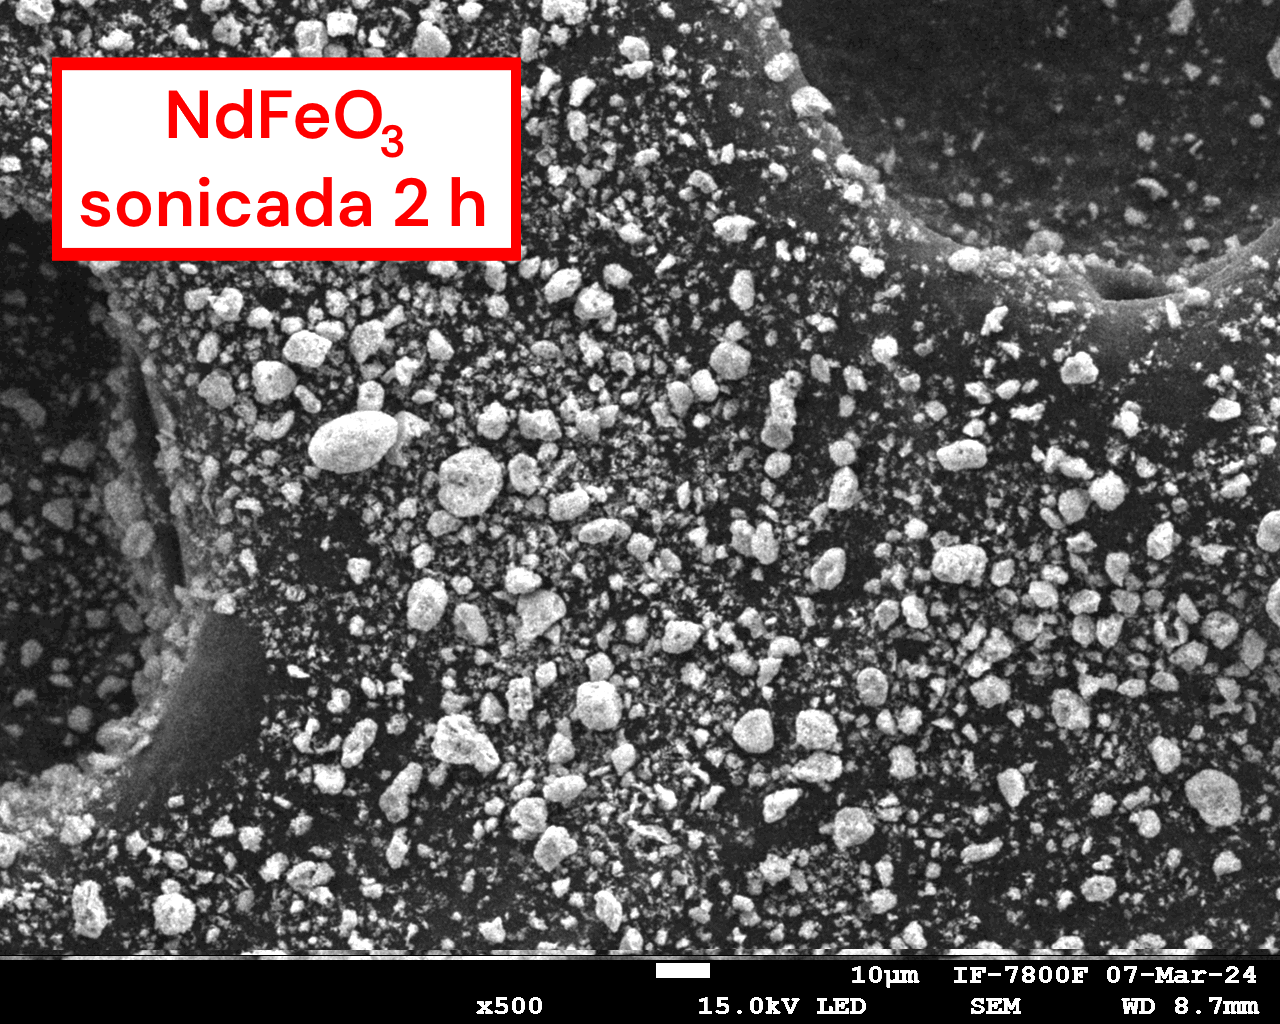
\includegraphics[width=0.45\textwidth]{fig/semneod2h.png}
    \quad
    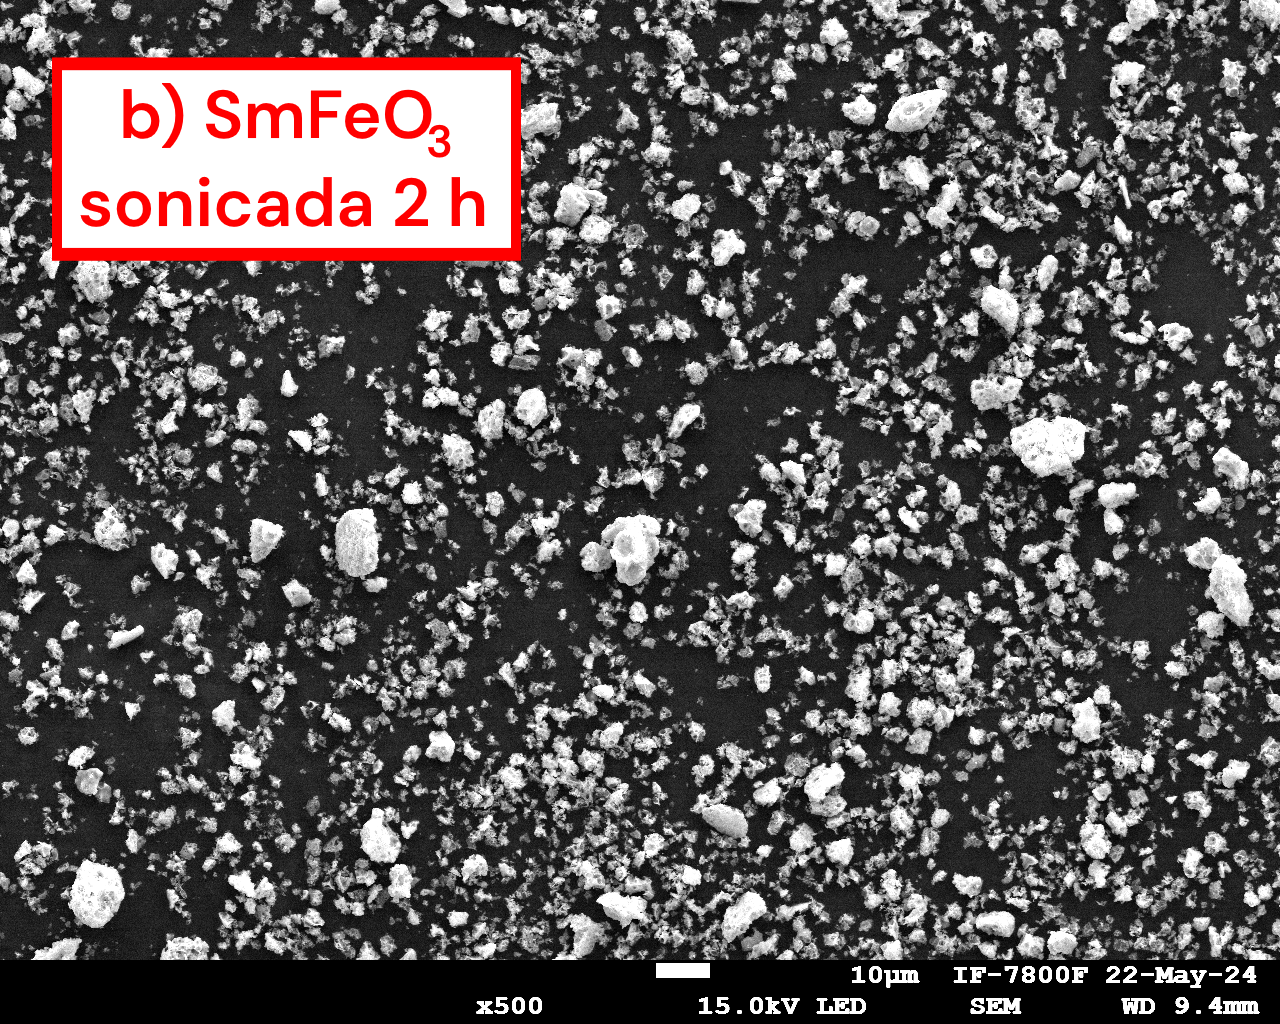
\includegraphics[width=0.45\textwidth]{fig/semsama2h.png}
    \caption{Imágenes obtenidas a través de SEM para las muestras sonicadas 2 horas. Muestra de a) \neod{} calcinada a 600\gradoC{}, b) \sama{} calcinada a 700\gradoC{}. Amplificación $\times500$}
    \label{fig:resSEMsonicada2}
\end{figure}
\begin{figure}[H]
    \centering
    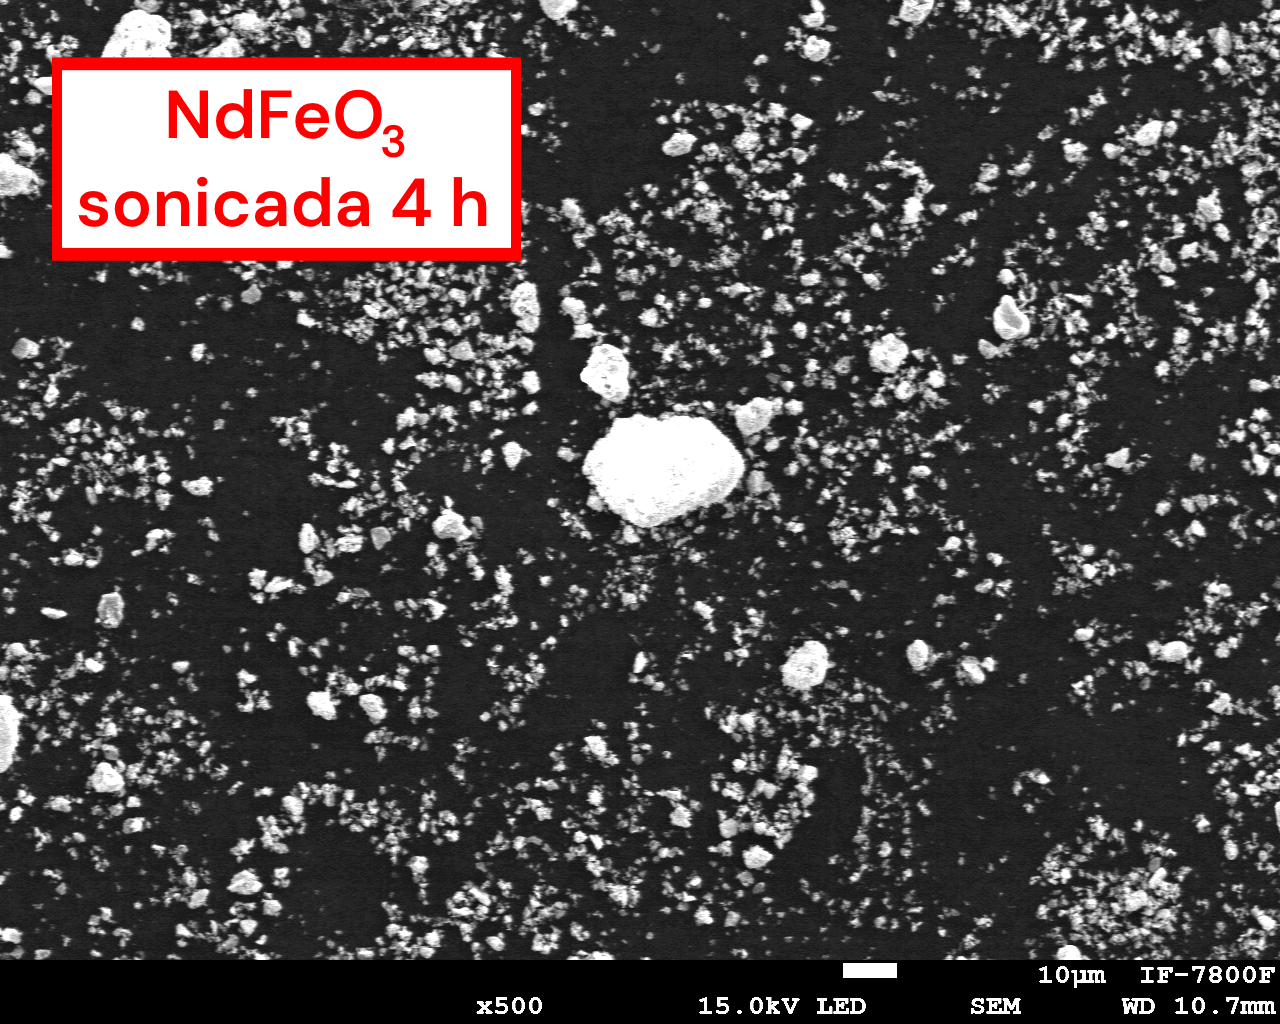
\includegraphics[width=0.45\textwidth]{fig/semneod4h.png}
    \quad
    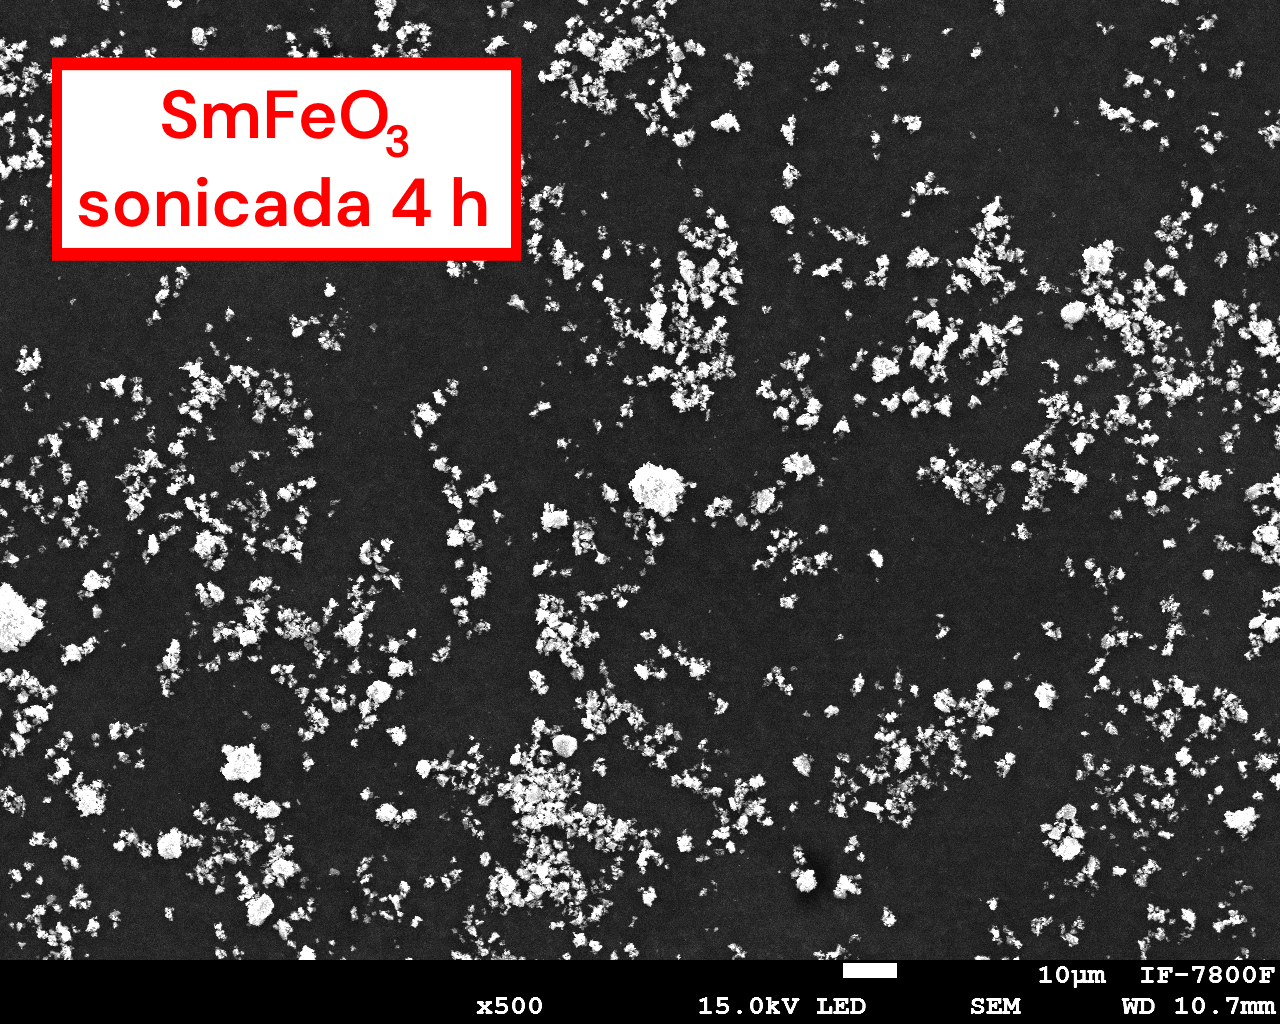
\includegraphics[width=0.45\textwidth]{fig/semsama4h.png}
    \caption{Imágenes obtenidas a través de SEM para las muestras sonicadas 4 horas. a) \neod{} calcinada a 600\gradoC{}, b) \sama{} calcinada a 700\gradoC{}. Amplificación $\times500$}
    \label{fig:resSEMsonicada4}
\end{figure}
Se observa que estas partículas presentan una estructura porosa independientemente de la temperatura, la cual se rompe después de ser sometida a un proceso de sonicación, siendo esto visible a simple vista al comparar las imágenes de las figuras \ref{fig:resSEMsinsonicar} y \ref{fig:resSEM900}, las cuales muestran a las ortoferritas de \neod{} calcinada a 600\gradoC{} y \sama{} calcinada a 700\gradoC{} respectivamente, con las que se encuentran en la figura \ref{fig:resSEMsonicada2}, en donde se muestran éstas mismas muestras después de ser sonicadas por 2 horas a 292W, además de las de la figura figura \ref{fig:resSEMsonicada4}, donde éstas muestras fueron sonicadas por 4 horas a la misma potencia.
Como ya se describió en la sección \ref{sec:analisisestadistico}, los tamaños de partícula fueron obtenidos haciendo uso de \textit{ImageJ}.

Los métodos descritos en esa sección dieron como resultado los siguientes resultados:
\begin{table}[H]
    \centering
    \begin{tabular}{|c||c|c|c|}
        \hline
        Muestra & Temperatura de & Diámetro promedio & Porcentaje \\
        & calcinación & ($\mu$m) & $\leq1$ $\mu$m (\%) \\
        \hline
        \hline
        \multirow{6}{*}{\rotatebox[origin=c]{90}{\neod{}}} & 600\gradoC{} & 1.49$\pm$0.028 & 67.29$\pm$4.079 \\
        \cline{2-4}
        & 600\gradoC{}, sonicada 2 h & 1.00$\pm$0.035 & 80.87$\pm$0.799 \\
        \cline{2-4}
        & 600\gradoC{}, sonicada 4 h & 0.98$\pm$0.023 & 87.10$\pm$1.292 \\
        \cline{2-4}
        & 700\gradoC{} & 1.76$\pm$0.047 & 58.80$\pm$1.841 \\
        \cline{2-4}
        & 800\gradoC{} & 2.5$\pm$0.087 & 61.27$\pm$1.805 \\
        \cline{2-4}
        & 900\gradoC{} & 2.66$\pm$0.065 & 53.85$\pm$2.558 \\
        \hline
        \hline
        \multirow{6}{*}{\rotatebox[origin=c]{90}{\sama{}}} & 700\gradoC{} & 2.01$\pm$0.051 & 55.18$\pm$2.103 \\
        \cline{2-4}
        & 700\gradoC{}, sonicada 2 h & 1.81$\pm$0.037 & 88.13$\pm$1.080 \\
        \cline{2-4}
        & 700\gradoC{}, sonicada 4 h & 1.66$\pm$0.045 & 92.62$\pm$0.915 \\
        \cline{2-4}
        & 800\gradoC{} & 1.91$\pm$0.034 & 44.4$\pm$2.504 \\
        \cline{2-4}
        & 900\gradoC{} & 1.97$\pm$0.029 & 62.28$\pm$2.498 \\
        \cline{2-4}
        & 1000\gradoC{} & 2.02$\pm$0.055 & 44.46$\pm$2.640 \\
        \hline
\end{tabular}
    \caption{Tamaño promedio de partícula y porcentaje de partículas con diámetro $\leq$1 $\mu$m según la temperatura de calcinación para ambas ferritas.}
    \label{tabla:restamañoprom}
\end{table}
\begin{figure}[H]
    \centering
    \includegraphics[width=0.9\textwidth]{fig/restamañoprom.png}
    \caption{Gráfica del tamaño promedio de partícula según la temperatura de calcinación. a) Muestras de \neod{}, b) muestras de \sama{}}
    \label{fig:restamañoprom}
\end{figure}
\begin{figure}[H]
    \centering
    \includegraphics[width=0.9\textwidth]{fig/resporcentaje.png}
    \caption{Gráfica del porcentaje de partículas con diámetro $\leq$1 $\mu$m según la temperatura de calcinación. a) Muestras de \neod{}, b) muestras de \sama{}}
    \label{fig:resporcentaje}
\end{figure}
Estos datos sugieren que el tamaño de partícula aumenta con la temperatura de calcinación, en particular para el \neod{}.

Por otro lado, la sonicación reduce considerablemente el tamaño promedio de partícula, además de aumentar el porcentaje de partículas con diámetro $\leq$1 $\mu$m

Sin embargo, duplicar el tiempo de sonicación no cambia los resultados de manera significativa, por lo cual se piensa que este proceso sólo rompe las partículas más grandes, pero no es lo suficientemente potente para fragmentar las más pequeñas.
\subsection{Espectroscopía de dispersión de energía}
Esta técnica reveló los elementos presentes en las muestras introducidas al microscopio electrónico de barrido, lo cual permite hallar posibles contaminantes, además de delimitar las posibles estructuras cristalinas a tomar en cuenta en el análisis de la difracción de rayos X de la sección \ref{sec:analisisDRX}.

En ninguna de las mediciones se encontraron contaminantes externos, a excepción de carbono, el cuál puede explicarse debido a que la cinta utilizada para la preparación de muestras está hecha de este material, como se muestra en las figuras \ref{fig:resEDSNeod} y \ref{fig:resEDSSama}. Esto se reporta en las tablas \ref{tab:EDSNd} y \ref{tab:EDSSm}.
\begin{figure}[H]
    \centering
    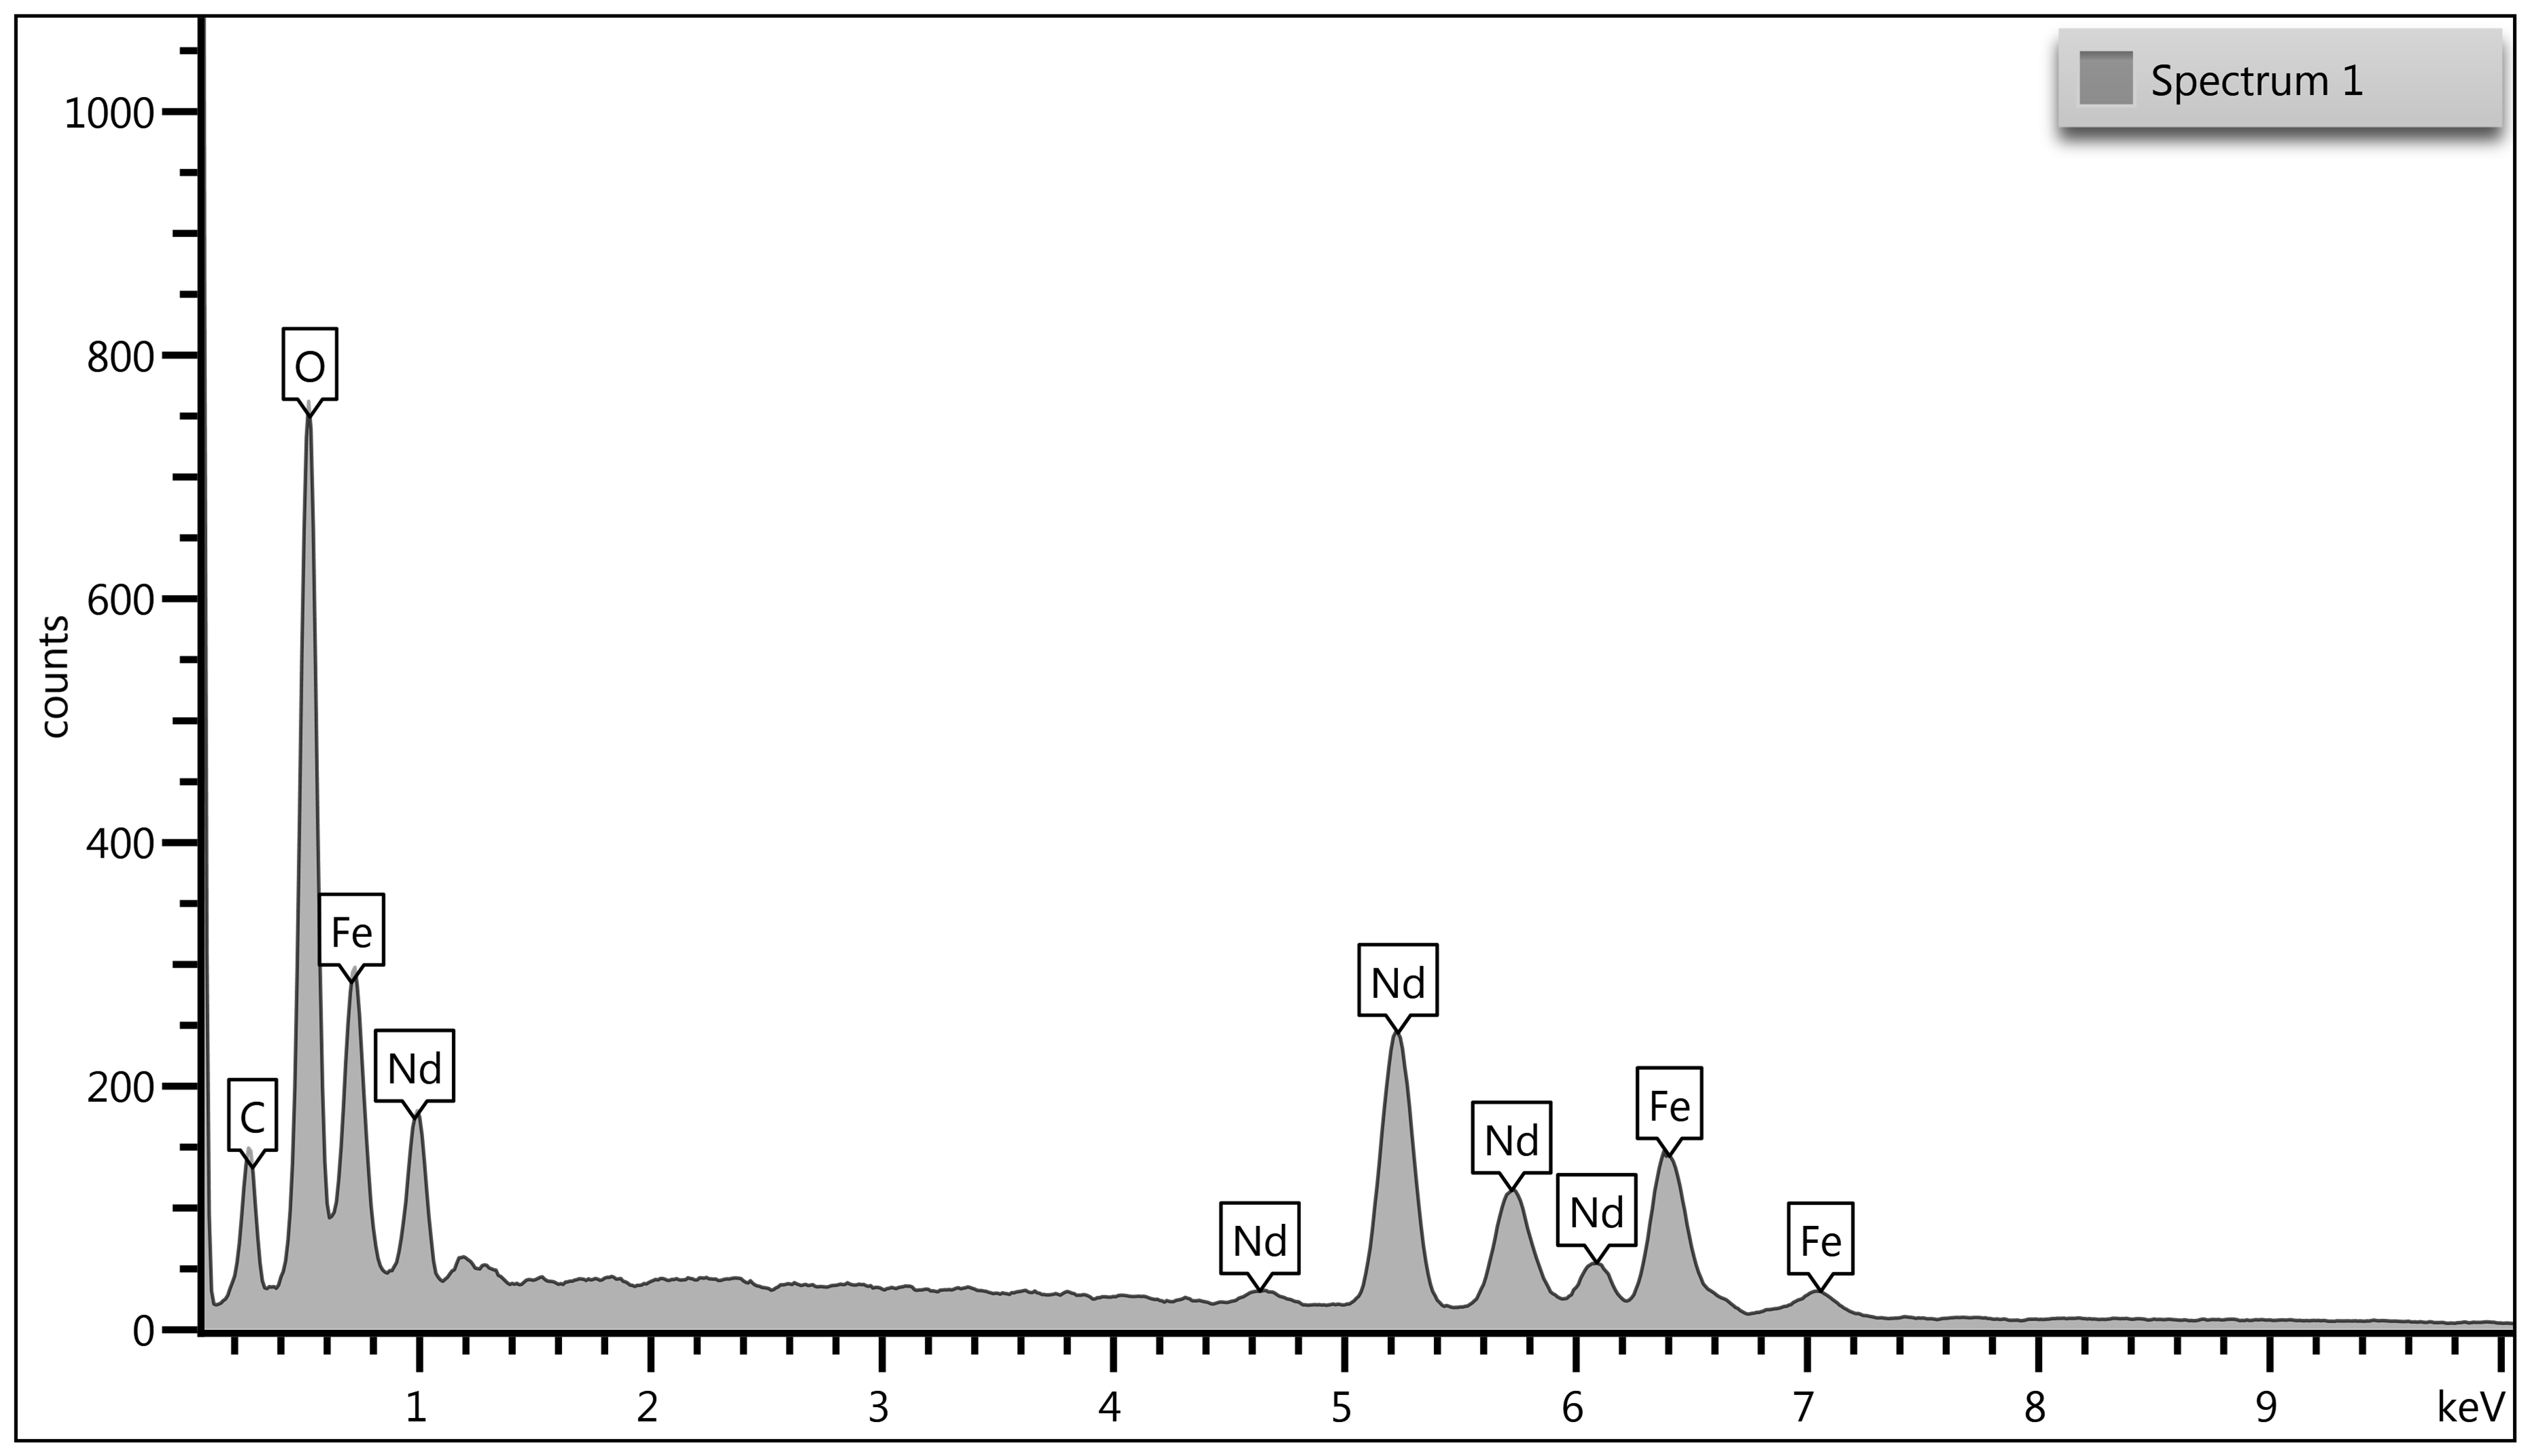
\includegraphics[width=0.7\textwidth]{fig/resEDSNeod.png}
    \caption{EDS de la muestra de \neod{} calcinada a 600\gradoC{} sin sonicar.}
    \label{fig:resEDSNeod}
\end{figure}
\begin{table}[H]
    \begin{tabular}{|c||c|c|c|c|c|c|c|}
        \hline
        Elem. &600\gradoC{} Son.&600\gradoC{} Son.&600\gradoC{}&700\gradoC{}&800\gradoC{}&900\gradoC{}&1000\gradoC{}\\
        &2h wt\%&4h wt\%&wt\%&wt\%&wt\%&wt\%&wt\%\\
        \hline\hline
        Fe & 20.33$\pm$0.78 &21.00$\pm$0.77& 19.94$\pm$0.68 & 22.23$\pm$1.01 & 20.31$\pm$0.67 & 21.0$\pm$1.04 & 18.37$\pm$2.06 \\
        Nd & 47.88$\pm$0.92 &58.44$\pm$0.87& 50.45$\pm$0.85 & 58.93$\pm$1.21 & 56.47$\pm$0.83 & 44.7$\pm$1.18 & 78.72$\pm$2.12 \\
        O & 31.79$\pm$0.70 &20.56$\pm$0.56& 21.71$\pm$0.54 & 11.04$\pm$0.57 & 15.06$\pm$0.45 & 20.4$\pm$0.57 & 2.92$\pm$0.60 \\
        C & 0 & 0 & 7.91$\pm$0.64 & 7.8$\pm$0.82 & 8.16$\pm$0.56 & 13.4$\pm$0.67 &0 \\ 
        \hline
        \end{tabular} 
            \caption{EDS de las muestras de \neod{}.}
            \label{tab:EDSNd}
        \end{table}
\begin{figure}[H]
    \centering
    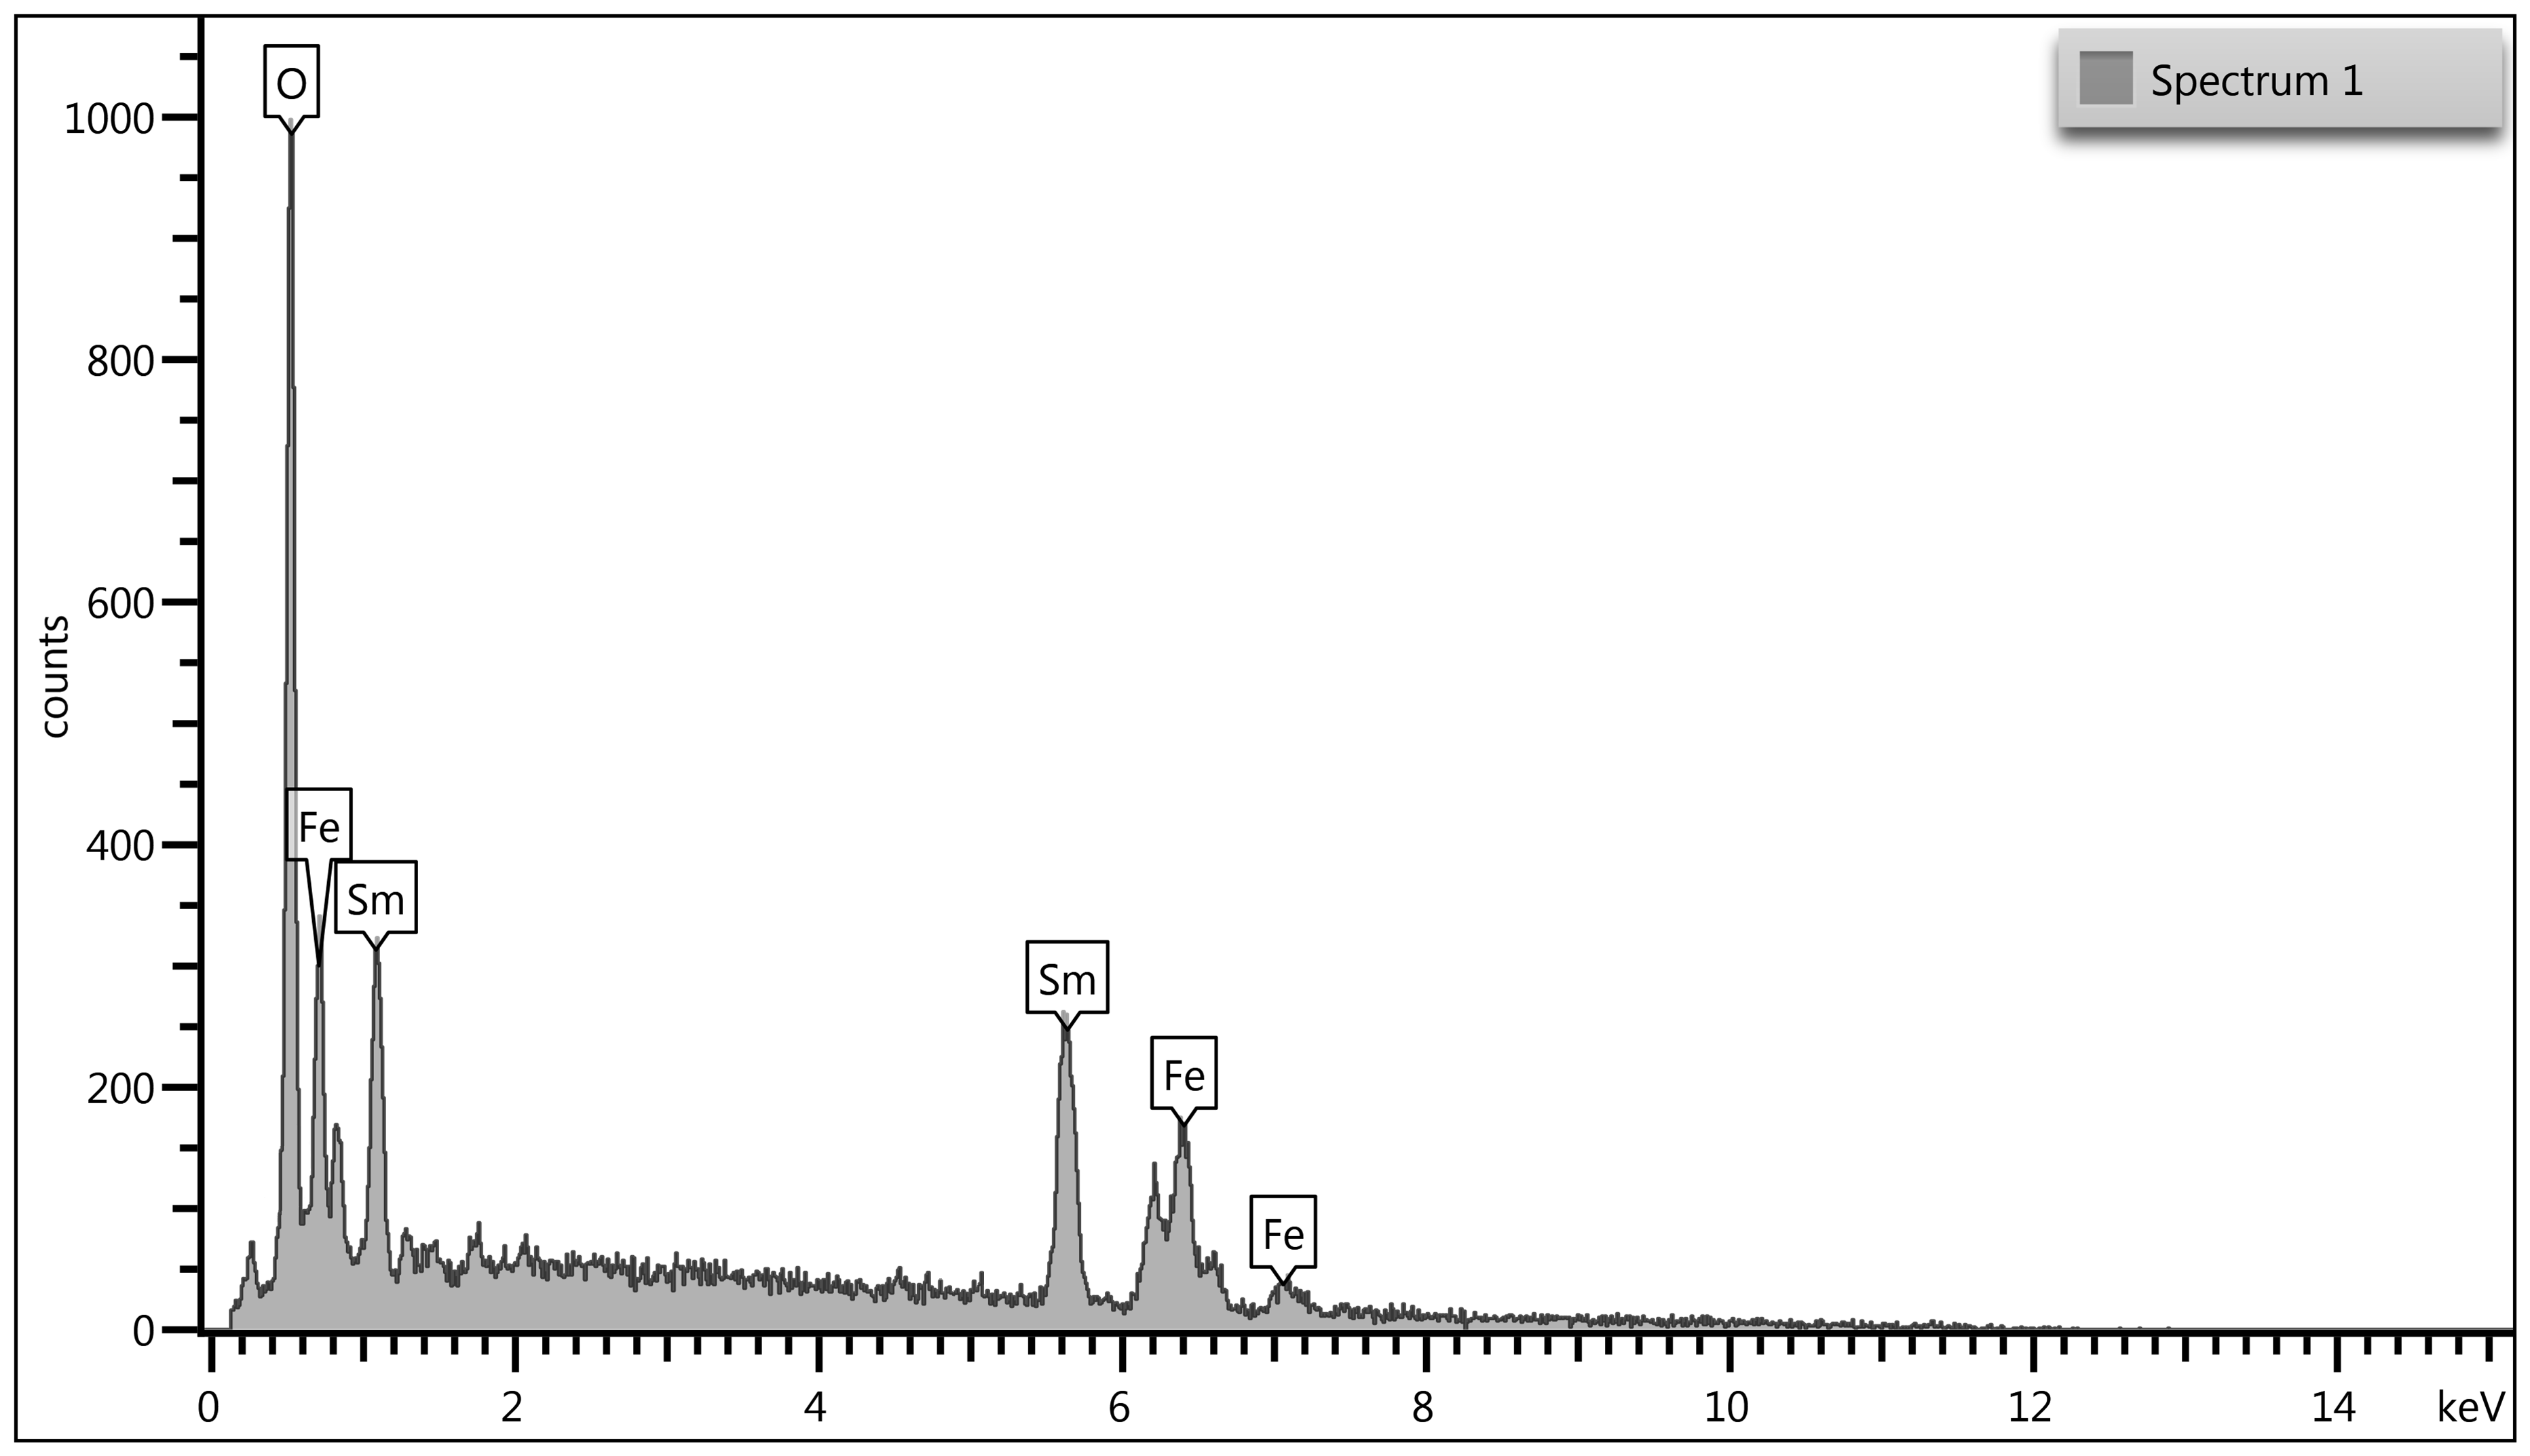
\includegraphics[width=0.7\textwidth]{fig/resEDSSama.png}
    \caption{EDS de la muestra de \sama{} calcinada a 700\gradoC{} sin sonicar.}
    \label{fig:resEDSSama}
\end{figure}
        \begin{table}[H]
            \centering
        \begin{tabular}{|c||c|c|c|c|c|c|}
        \hline
        Elem. &700\gradoC{} Son.&700\gradoC{} Son.&700\gradoC{}&800\gradoC{}&900\gradoC{}&1000\gradoC{}\\
        &2h wt\%&4h wt\%&wt\%&wt\%&wt\%&wt\%\\
        \hline\hline
        Fe &13.78$\pm$0.52&19.48$\pm$1.48& 7.51$\pm$0.42 & 22.31$\pm$0.93 & 22.51$\pm$3.03 & 17.44$\pm$0.83 \\
        Sm &38.42$\pm$0.74&48.22$\pm$1.95& 21.84$\pm$0.69 & 61.28$\pm$1.03 & 63.03$\pm$3.57 & 57.71$\pm$1.82 \\
        O &18.74$\pm$0.45&15.64$\pm$1.00& 15.95$\pm$0.47 & 16.41$\pm$0.58 & 14.46$\pm$1.78 & 20.81$\pm$0.78 \\
        C &29.16$\pm$0.62&16.66$\pm$1.53& 0 & 54.68$\pm$0.77 & 0 & 4.13$\pm$2.17 \\ 
        \hline
        \end{tabular} 
            \caption{EDS de las muestras de \sama{}.}
            \label{tab:EDSSm}
\end{table}
\subsection{Difracción de rayos X} \label{sec:analisisDRX}
A continuación se reportan los espectros obtenidos mediante la metodología descrita en \ref{sec:metodologiadrx} para cada temperatura de calcinación.
\begin{figure}[H]
    \centering
    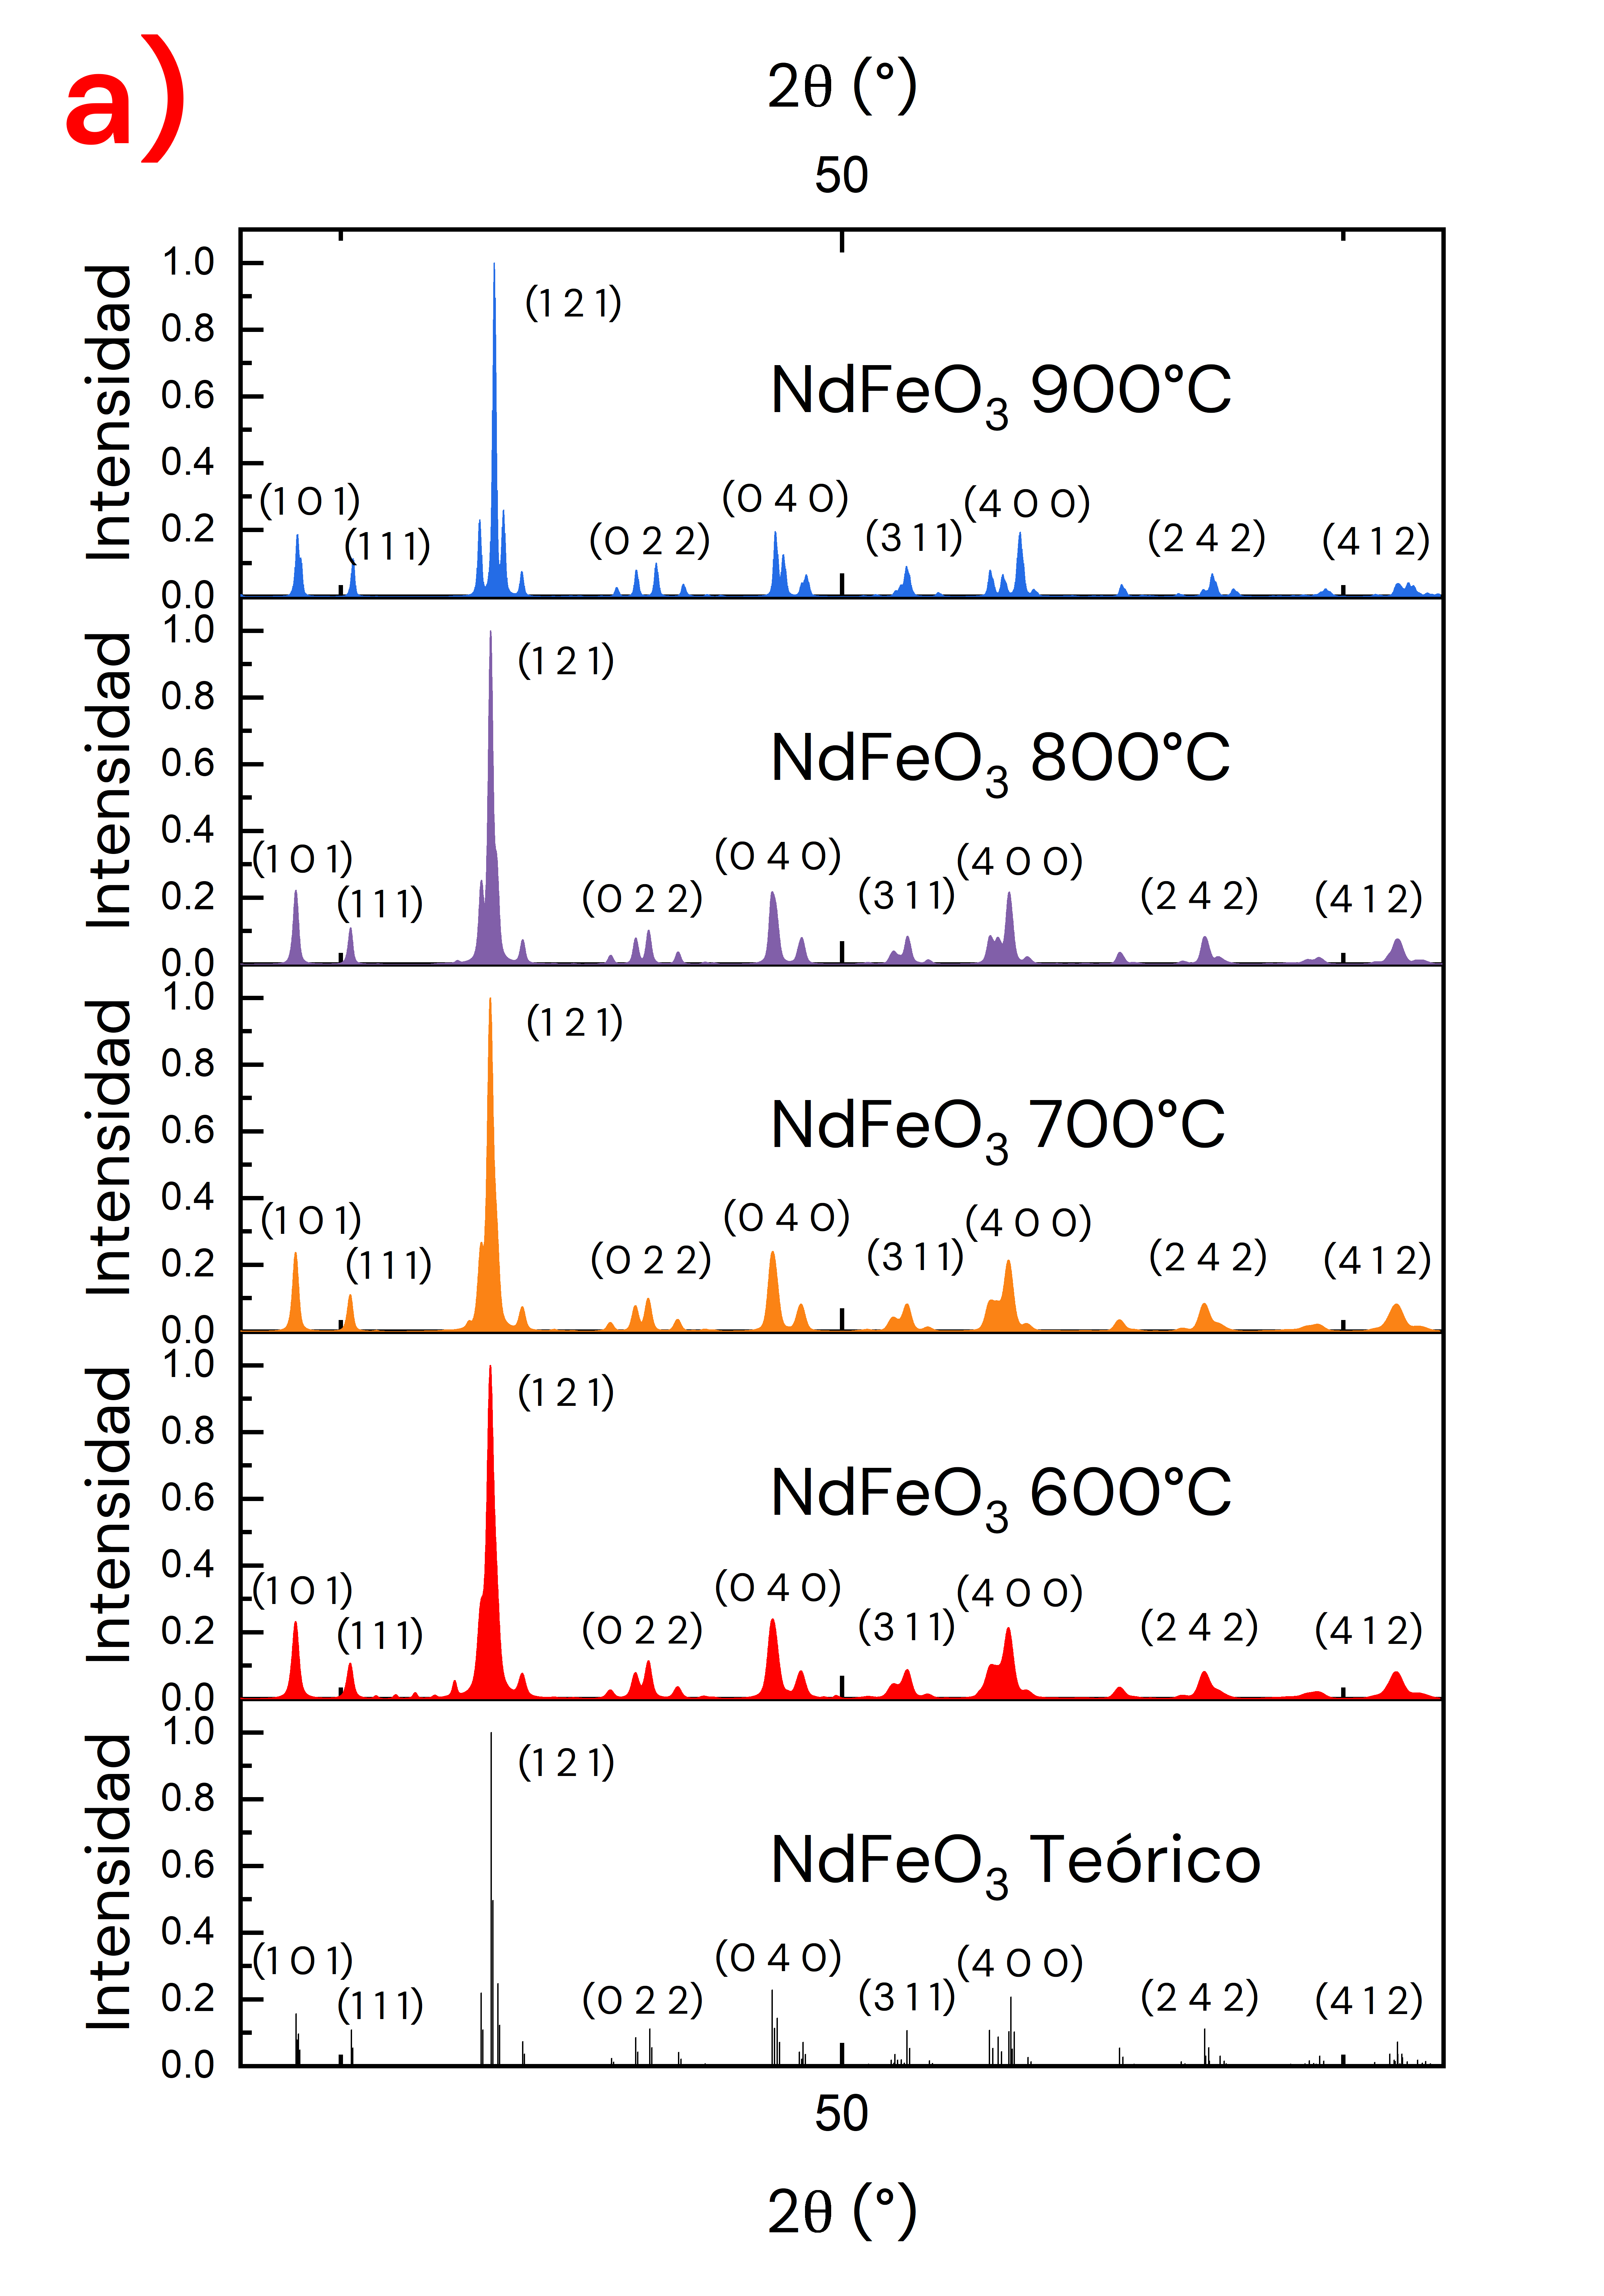
\includegraphics[width=0.45\textwidth]{fig/drxtempndfeo3.png}
    \quad
    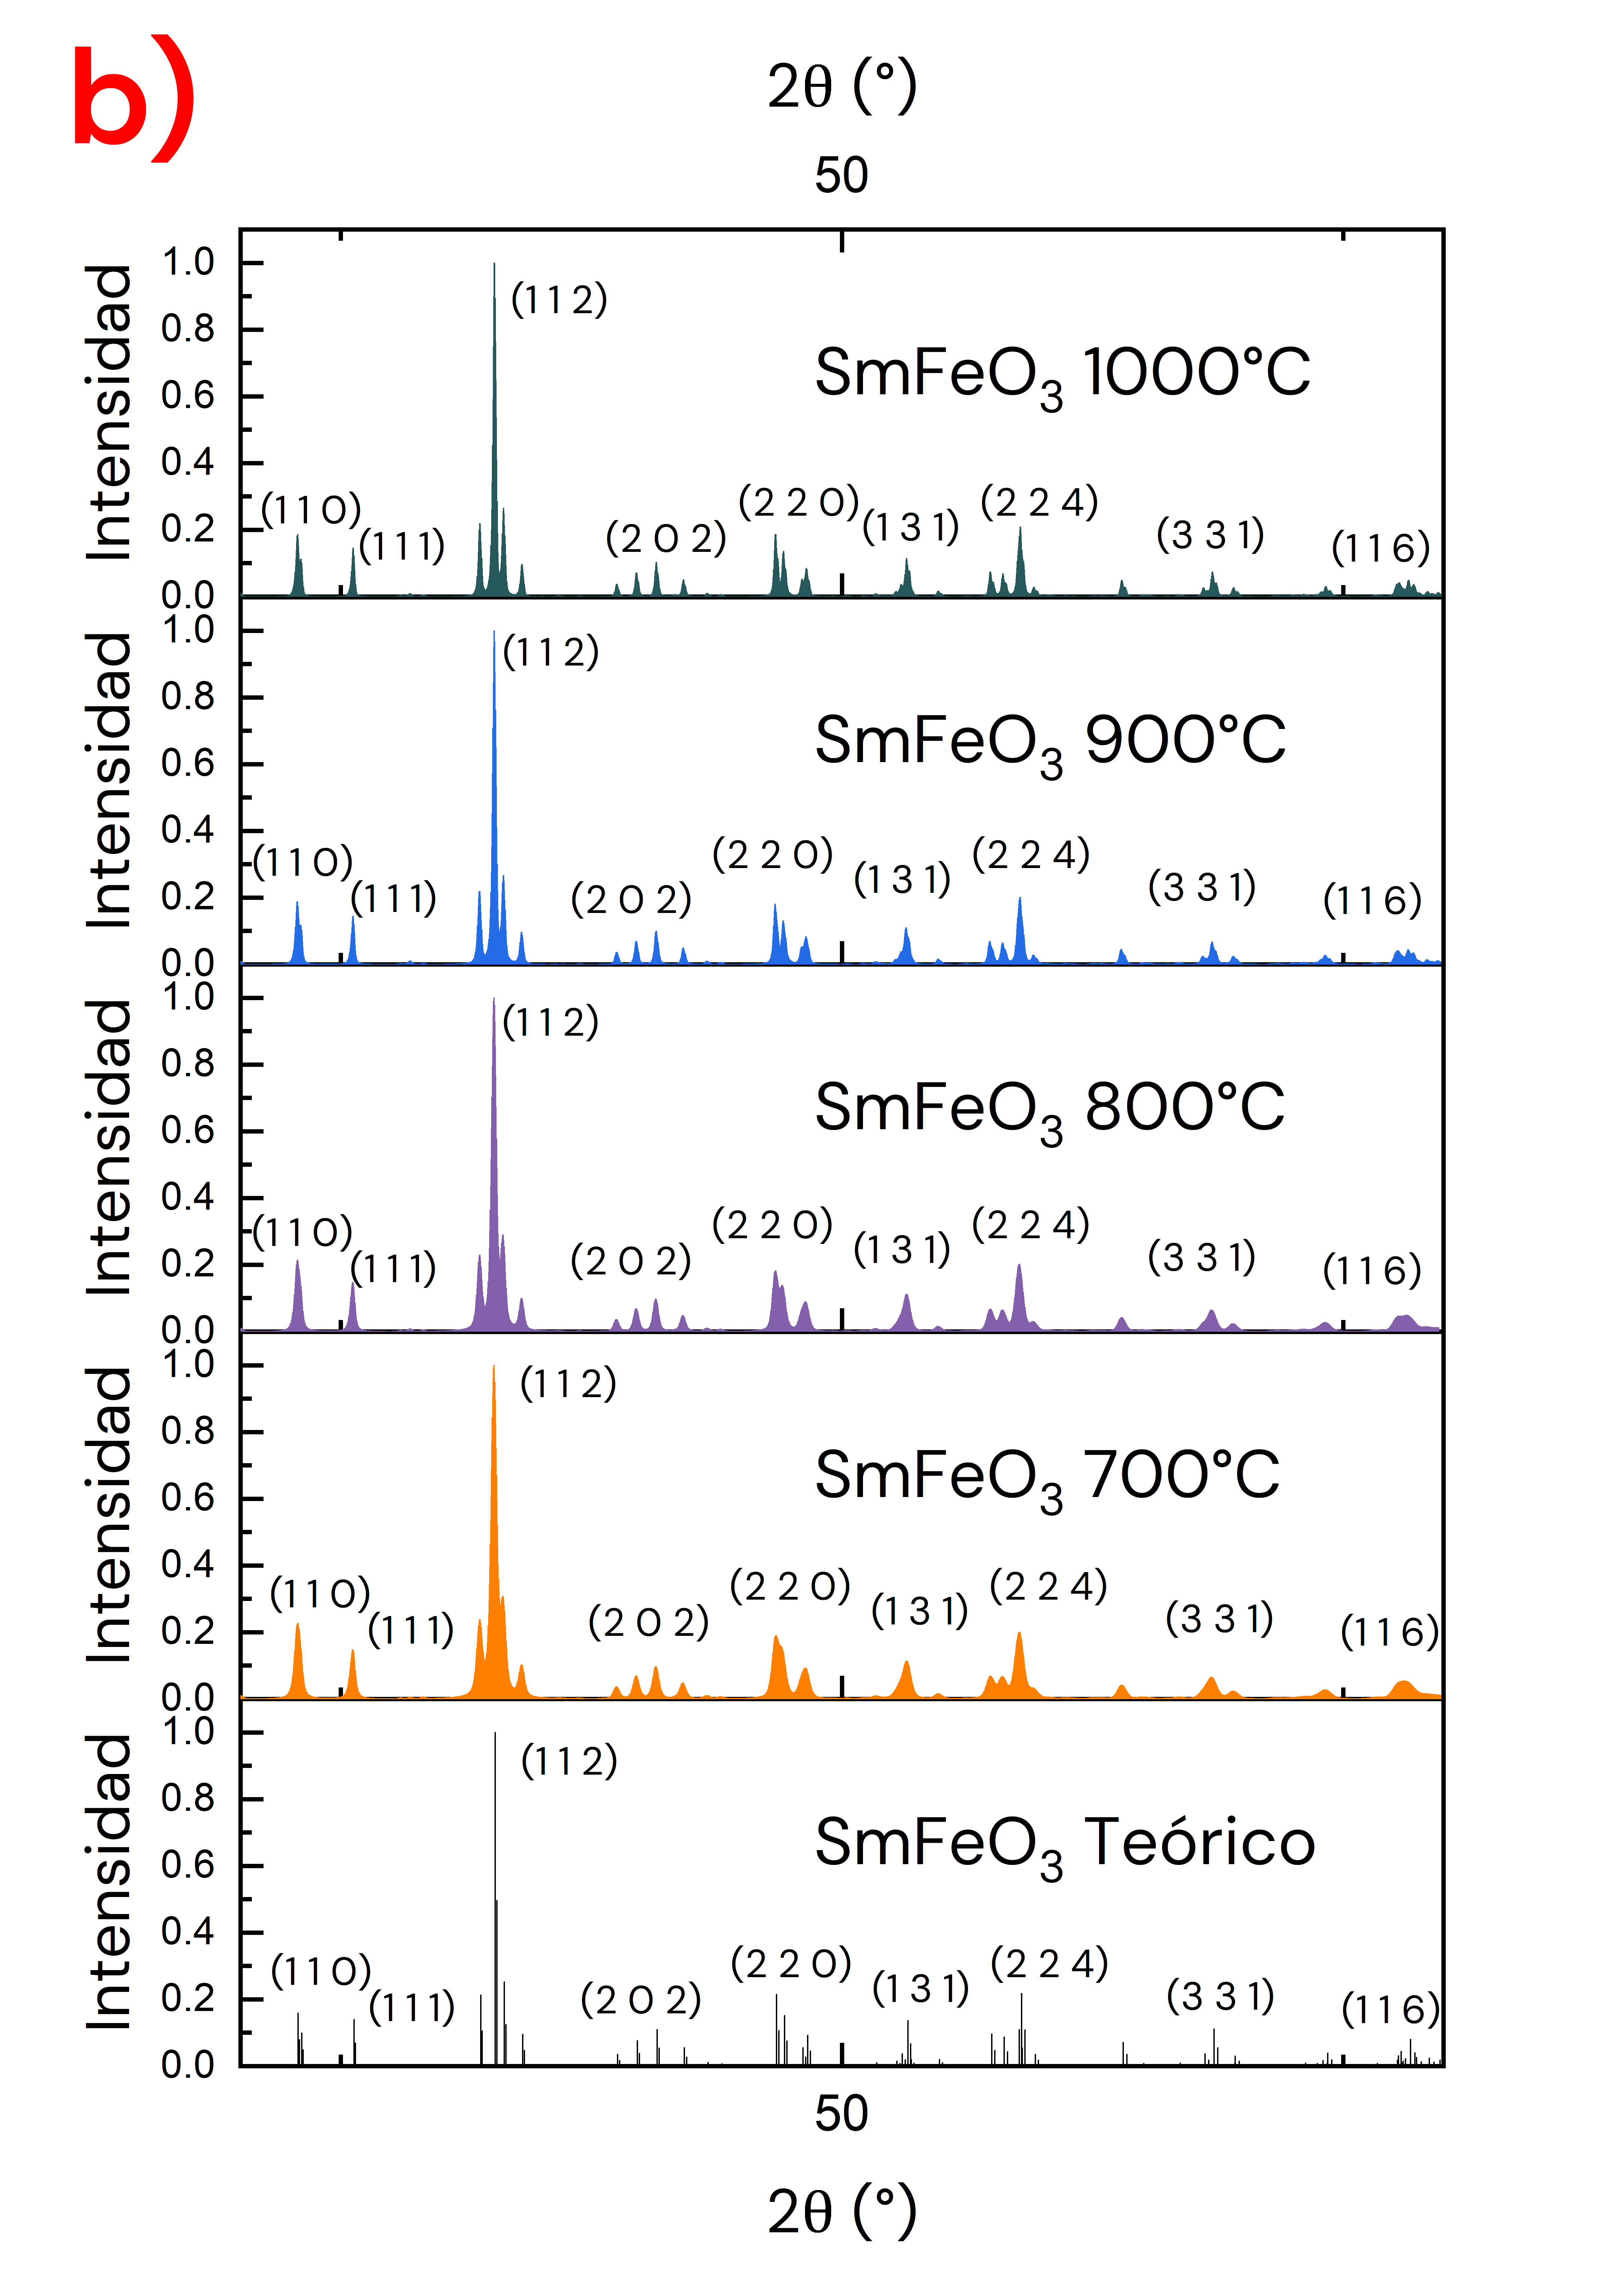
\includegraphics[width=0.45\textwidth]{fig/drxtempsmfeo3.png}
    \caption{Espectros obtenidos mediante DRX de las muestras calcinadas a distintas temperaturas. a) Muestras de \neod{}, b) Muestras de \sama{}. En cada gráfica se indican entre paréntesis los ángulos de difracción para diferentes planos obtenidos de \cite{ndfeo3} y \cite{smfeo3} respectivamente, así como la temperatura de calcinación de cada muestra.}
    \label{fig:drxtempcomp}
\end{figure}
Se puede observar que los picos obtenidos coinciden con el espectro de la estructura reportada en \cite{ndfeo3} para el \neod{} y en \cite{smfeo3} para el \sama{}.

Se observa el desdoblamiento del pico principal al aumentar la temperatura de calcinación entre 700 y 900\gradoC{}, especialmente para el \neod{}, esto sugiere un cambio de fase cristalina al realizar la síntesis a mayor temperatura.

A continuación se reportan los espectros obtenidos para las muestras sonicadas
\begin{figure}[H]
    \centering
    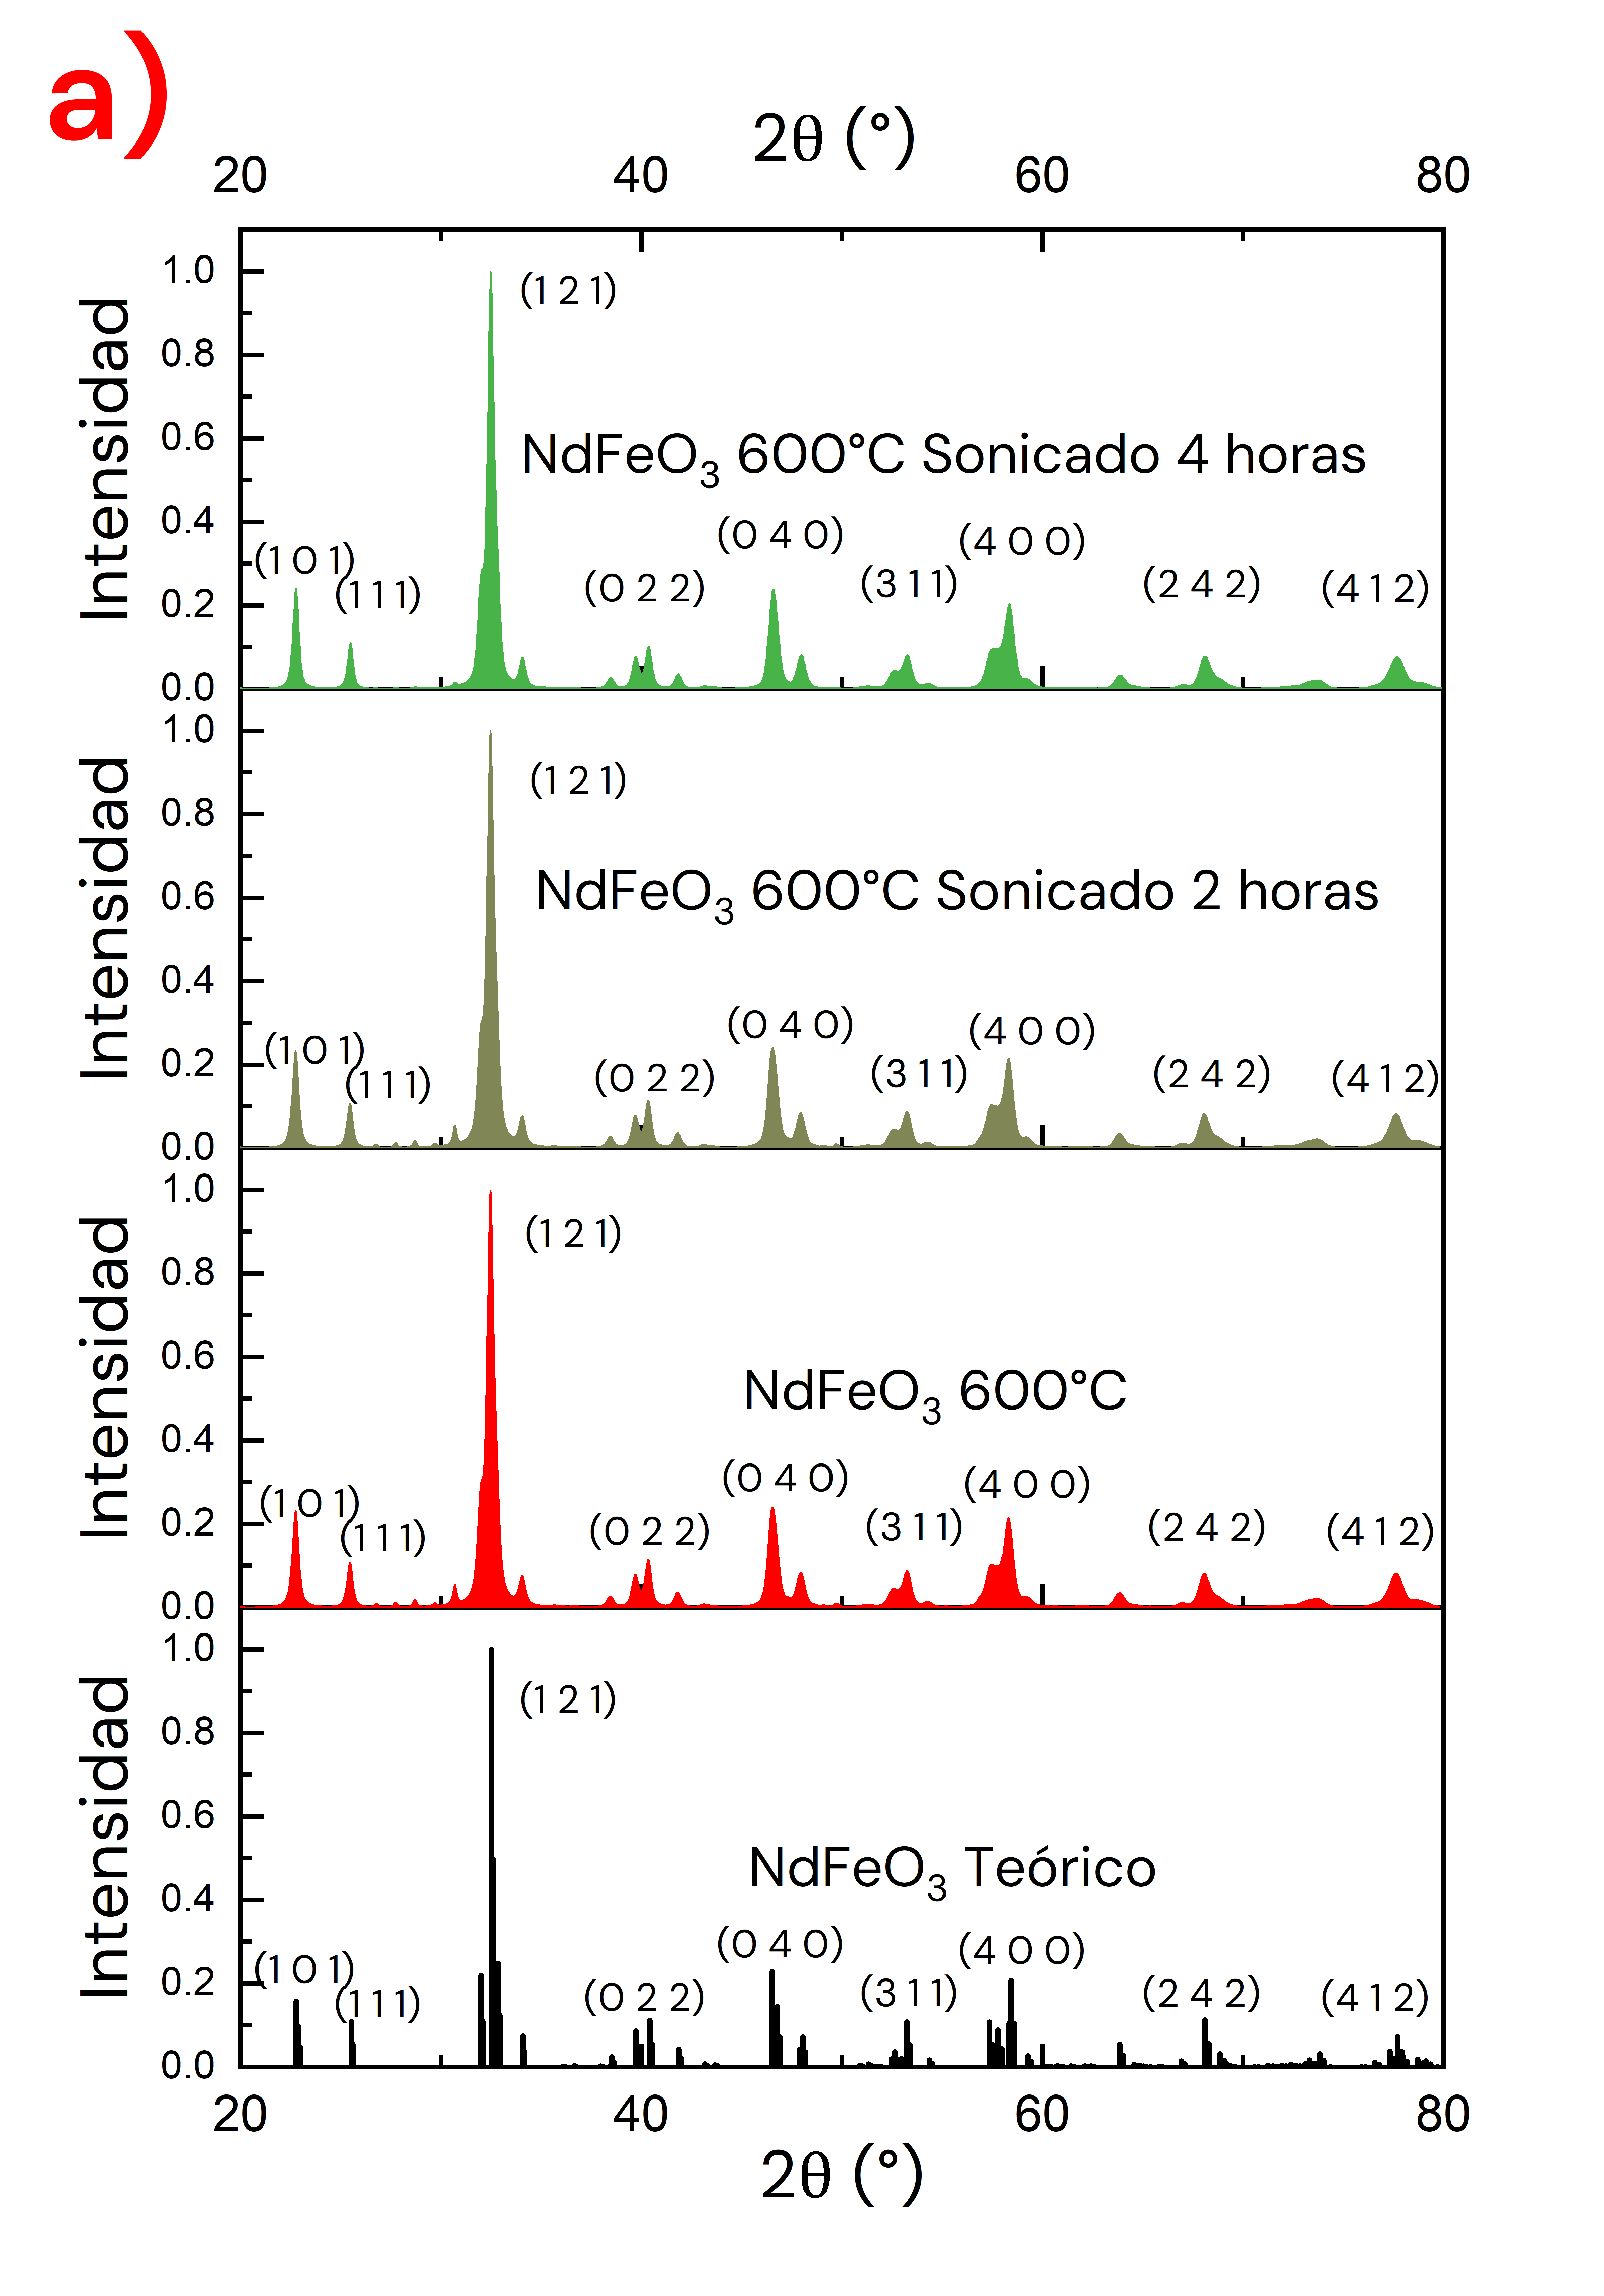
\includegraphics[width=0.45\textwidth]{fig/drxsonicndfeo3.png}
    \quad
    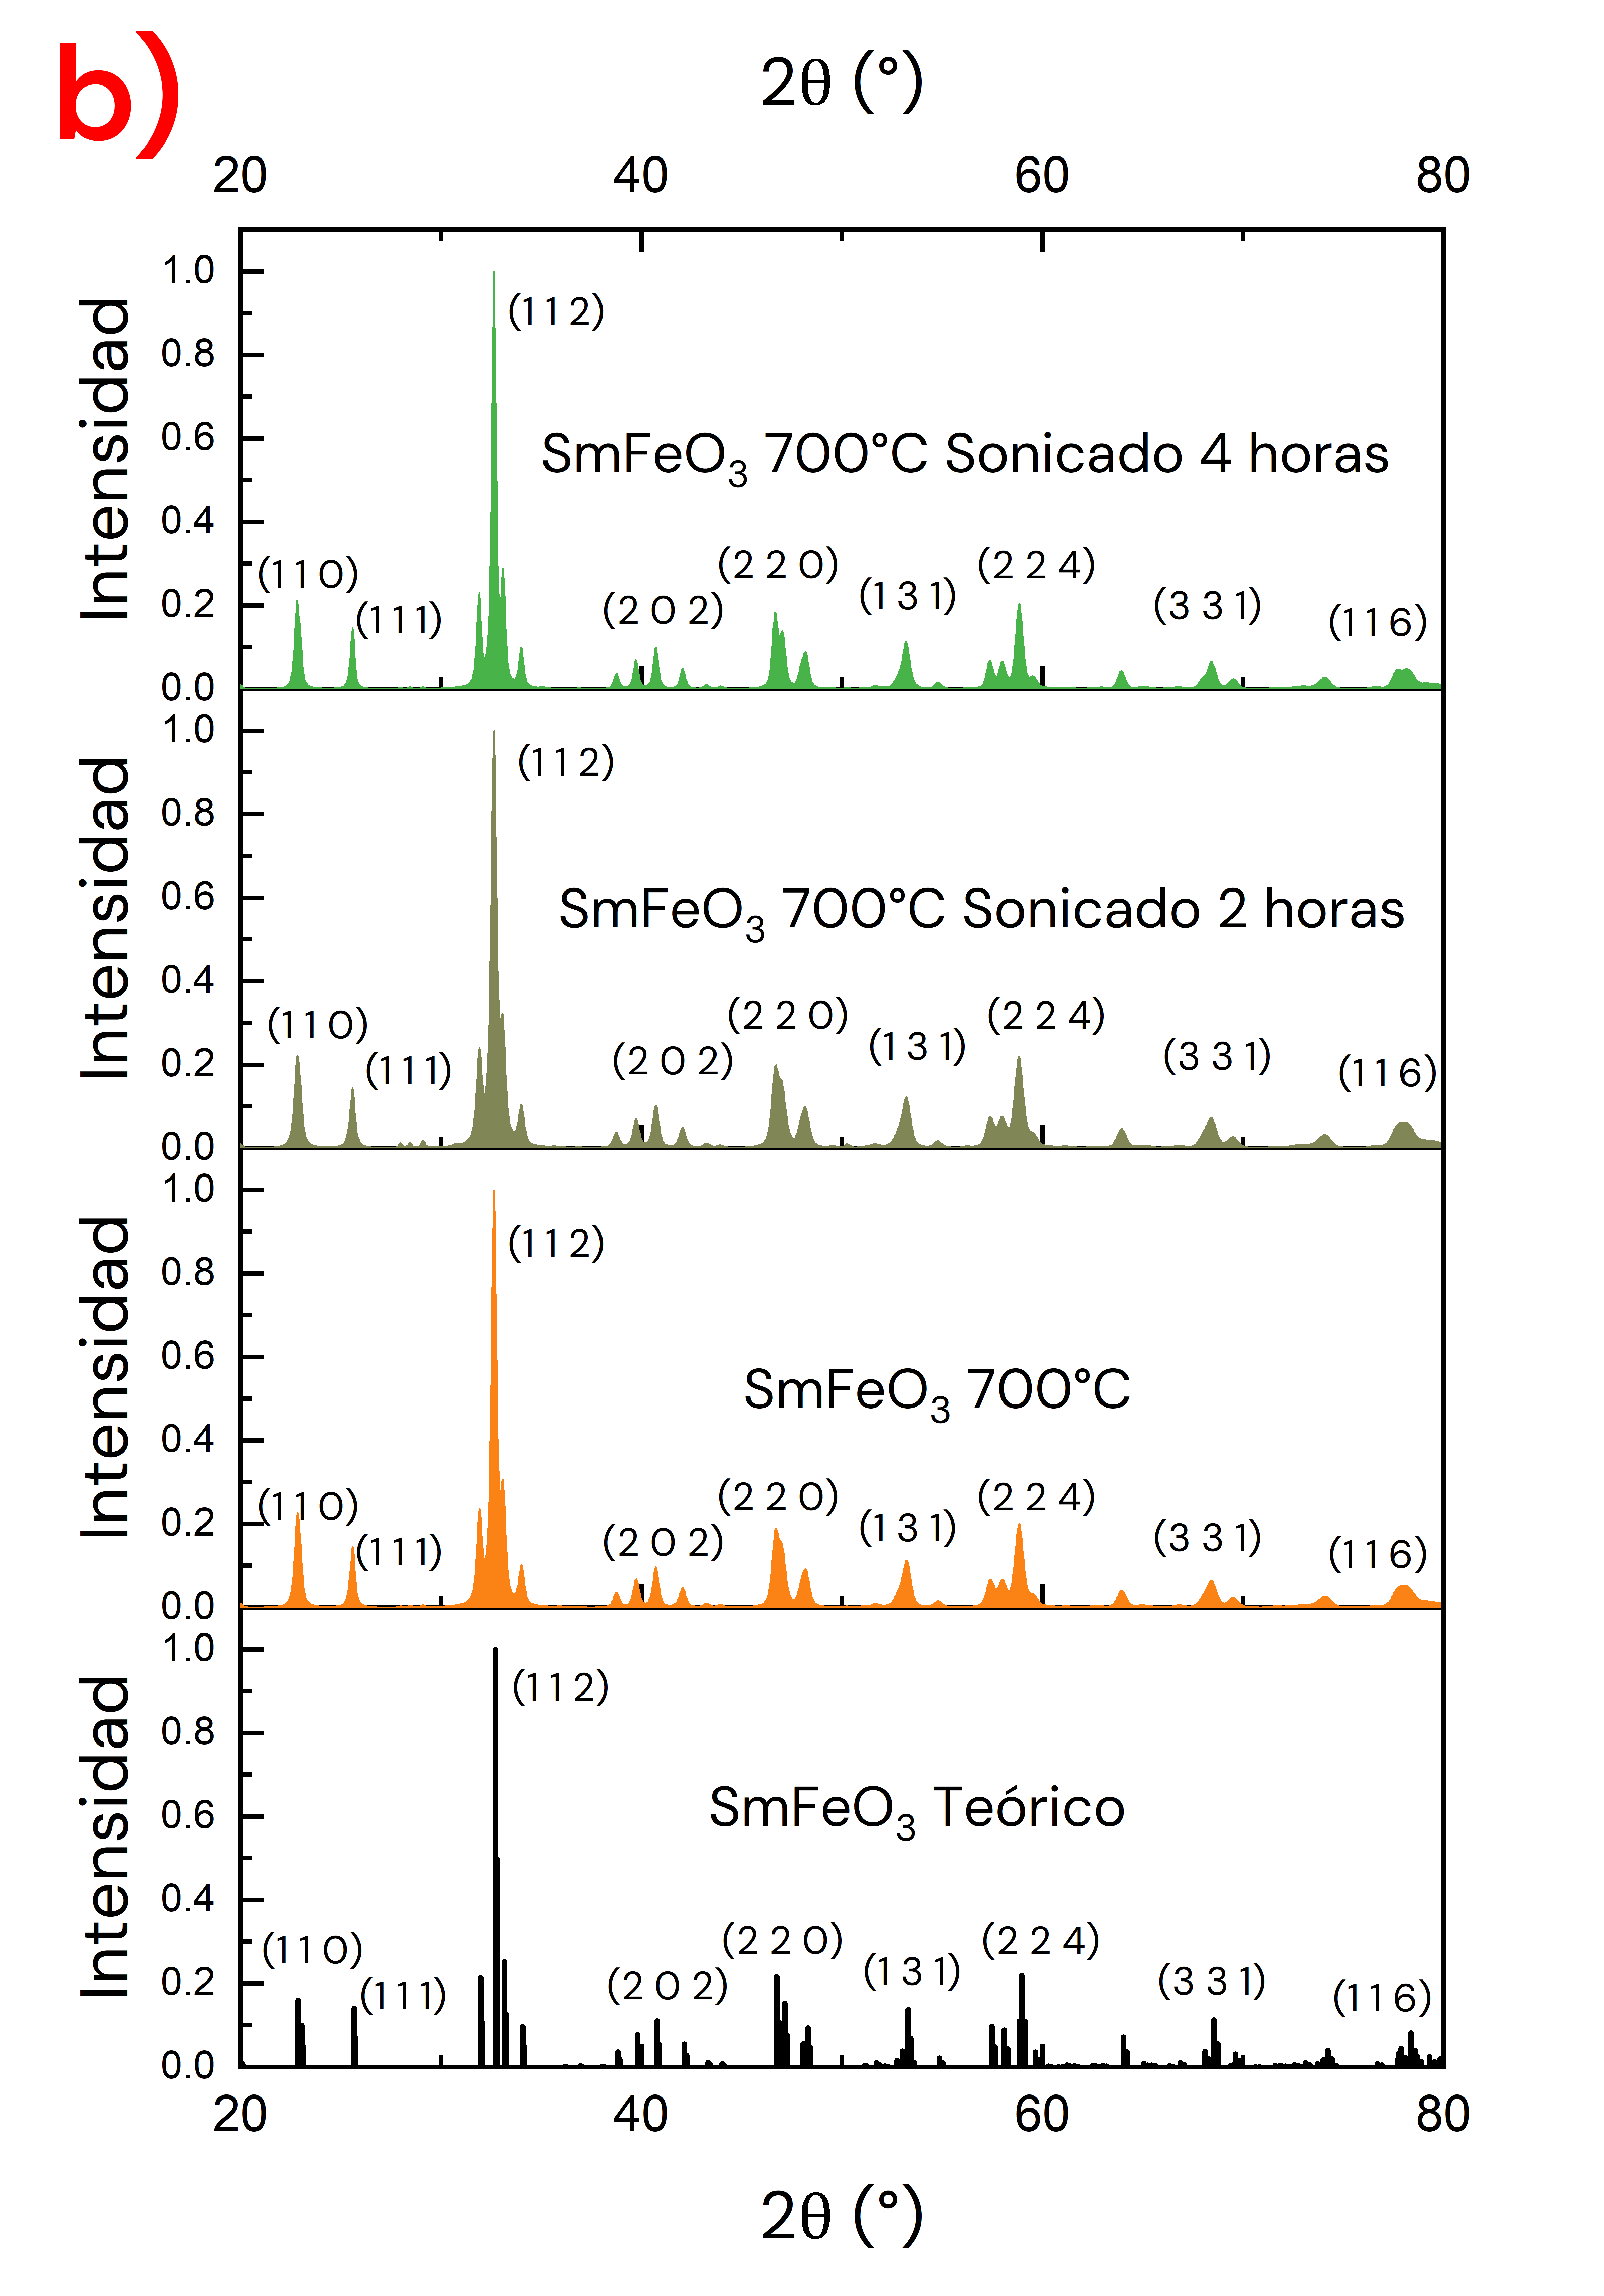
\includegraphics[width=0.45\textwidth]{fig/drxsonicsmfeo3.png}
    \caption{Espectros obtenidos mediante DRX de las muestras sonicadas. a) Muestras de \neod{}, b) Muestras de \sama{}. En cada gráfica se indican entre paréntesis los ángulos de difracción para diferentes planos obtenidos de \cite{ndfeo3} y \cite{smfeo3} respectivamente, así como el tiempo de sonicación de cada muestra.}
    \label{fig:drxsoniccomp}
\end{figure}
No se observan cambios notorios entre los espectros al variar el tiempo de sonicación, por lo que no parece haber un cambio en la estructura cristalina.

\subsubsection{Refinamiento Rietveld} \label{sec:resrietlveld}
Mediante esta técnica se obtuvieron los siguientes ajustes entre los espectros teóricos y los obtenidos experimentalmente (figura \ref{fig:rietveld600ndresultados} y \ref{fig:rietveld700smresultados}), así como un estimado del porcentaje del peso que representa cada fase cristalina presente en la muestra (tablas \ref{tabla:refrietvneod} y \ref{tabla:refrietvsama}):
\begin{figure}[H]
    \centering
    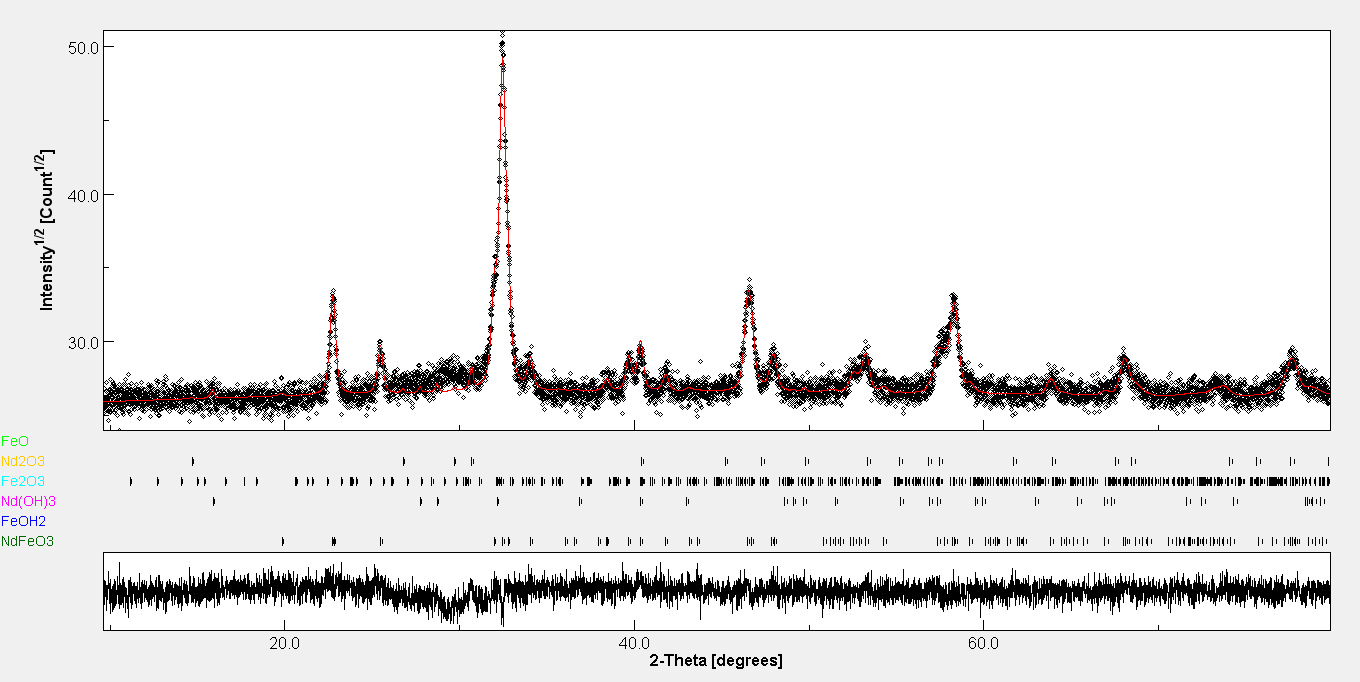
\includegraphics[width=0.8\textwidth]{fig/DRX600NdFeO3.png}
    \caption{Refinamiento Rietveld de la muestra de \neod{} calcinada a 600\gradoC{} sin sonicar. Los puntos negros son el espectro de difracción obtenido experimentalmente, la curva roja es el ajuste hecho por \textit{MAUD} (panel superior). Estructuras utilizadas: \neod{} \cite{ndfeo3}, \ce{Nd(OH)3} \cite{ndoh3}, \ce{Fe(OH)2} \cite{feoh2}, \ce{Nd2O3} \cite{nd2o3}, \ce{Fe2O3} \cite{fe2o3}, \ce{FeO} \cite{feo} (panel inferior).}
    \label{fig:rietveld600ndresultados}
\end{figure}
\begin{figure}[H]
    \centering
    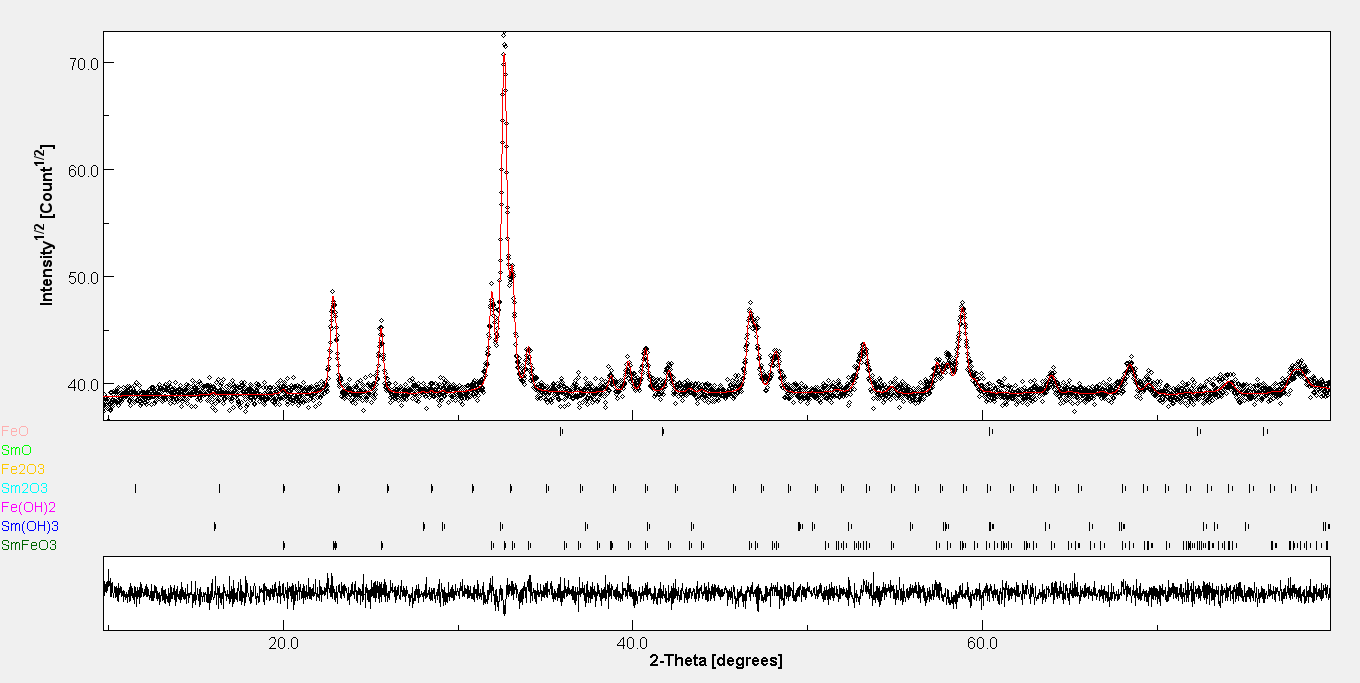
\includegraphics[width=0.8\textwidth]{fig/DRX700SmFeO3.png}
    \caption{Refinamiento Rietveld de la muestra de \neod{} calcinada a 600\gradoC{} sin sonicar. Los puntos negros son el espectro de difracción obtenido experimentalmente, la curva roja es el ajuste hecho por \textit{MAUD} (panel superior). Estructuras utilizadas: \sama{} \cite{smfeo3}, \ce{Sm(OH)3} \cite{smoh3}, \ce{Fe(OH)2} \cite{feoh2}, \ce{Sm2O3} \cite{sm2o3}, \ce{Fe2O3} \cite{fe2o3}, \ce{SmO} \cite{smo}, \ce{FeO} \cite{feo} (panel inferior).}
    \label{fig:rietveld700smresultados}
\end{figure}
El resto de refinamientos pueden encontrarse en el anexo \ref{sec:anexorietveld}.

Mediante estos refinamientos se encontró que las muestras contienen las siguientes composiciones en los porcentajes respectivos. Así mismo en la última columna se muestra el ajuste de bondad:
\begin{table}[H]
    \centering
    \begin{tabular}{|c||c|c|c|c|c|c|c|}
        \hline
        Muestra & \neod{} & \ce{Fe(OH)2} & \ce{Nd(OH)3} & \ce{Nd2O3} & \ce{Fe2O3} & \ce{FeO} & $\chi^2$ \\
        \hline
        \hline
        600\gradoC{} S 4 h & 98.81$\pm$0.0 & 0.61$\pm$0.782 & 0.26$\pm$0.170 & 0.30$\pm$0.111 & 0$\pm$0 & 0$\pm$0 & 1.08 \\
        \hline
        600\gradoC{} S 2 h & 95.73$\pm$0.0 & 0$\pm$0 & 1.38$\pm$0.231 & 2.62$\pm$0.188 & 0.24$\pm$0.649 & 0.00$\pm$0.309 & 1.21 \\
        \hline
        600\gradoC{} & 96.97$\pm$0.0 & 0$\pm$0 & 1.16$\pm$0.163 & 1.49$\pm$0.1312 & 0.37$\pm$0.457 & 0$\pm$0 & 1.12 \\
        \hline
        700\gradoC{} & 98.67$\pm$0.0 & 0$\pm$0 & 0$\pm$0 & 0.57$\pm$0.096 & 0.74$\pm$0.331 & 0$\pm$0 & 1.07 \\
        \hline
        800\gradoC{} & 98.67$\pm$0.0 & 0.40$\pm$0.632 & 0$\pm$0 & 0.33$\pm$0.088 & 0.58$\pm$0.319 & 0$\pm$0 & 1.05 \\
        \hline
        900\gradoC{} & 99.20$\pm$0.0 & 0$\pm$0 & 0$\pm$0 & 0.10$\pm$0.100 & 0.10$\pm$0.351 & 0.58$\pm$0.414 & 1.12 \\
        \hline
        \end{tabular} 
    \caption{Porcentaje del peso que representa cada una de las estructuras cristalinas presentes en cada muestra de \neod{}.}
    \label{tabla:refrietvneod}
\end{table}

\begin{table}[H]
    \centering
    \begin{tabular}{|c||c|c|c|c|c|c|c|}
        \hline
        Muestra & \sama{} & \ce{Sm(OH)3} & \ce{Fe(OH)2} & \ce{Sm2O3} & \ce{Fe2O3} & \ce{FeO} & $\chi^2$ \\ 
        \hline\hline
        700\gradoC{} S 4 h & 97.95$\pm$0.0 & 0.40$\pm$0.218 & 1.41$\pm$1.011 & 0.22$\pm$0.153 & 0$\pm$0 & 0$\pm$0 & 1.06 \\
        \hline
        700\gradoC{} S 2 h & 98.19$\pm$0.0 & 1.22$\pm$0.260 & 0$\pm$0 & 0.56$\pm$0.184 & 0$\pm$0 & 0$\pm$0 & 1.10 \\
        \hline
        700\gradoC{} & 99.17$\pm$0.0 & 0.35$\pm$0.176 & 0$\pm$0 & 0.19$\pm$0.150 & 0$\pm$0 & 0.27$\pm$0.358 & 1.07 \\
        \hline
        800\gradoC{} & 98.90$\pm$0.0 & 0.41$\pm$0.175 & 0$\pm$0 & 0.37$\pm$0.149 & 0$\pm$0 & 0.30$\pm$0.353 & 1.06 \\
        \hline
        900\gradoC{} & 98.65$\pm$0.0 & 0.41$\pm$0.178 & 0$\pm$0 & 0.69$\pm$0.151 & 0.23$\pm$0.484 & 0$\pm$0 & 1.08 \\
        \hline
        1000\gradoC{} & 97.56$\pm$0.0 & 0.70$\pm$0.177 & 0$\pm$0 & 0.64$\pm$0.149 & 0$\pm$0 & 1.08$\pm$0.348 & 1.09 \\
        \hline
        \end{tabular} 
    \caption{Porcentaje del peso que representa cada una de las estructuras cristalinas presentes en cada muestra de \sama{}.}
    \label{tabla:refrietvsama}
\end{table}
Se observa que el método de síntesis utilizado produce muestras de pureza alta, $\geq$95.73 para el \neod{} y $\geq$97.95 para el \sama{}. Por su parte, el valor de $\chi^2$ se encuentra en el rango establecido en \ref{sec:refinamiento} (1-1.3), teniendo como valor máximo 1.21, lo cual indica un buen ajuste en todos los refinamientos.

Por otro lado, los diámetros de cristal promedio se reportan en la tabla \ref{tabla:tamañoscristal}. Una gráfica de estos contra la temperatura de calcinación se encuentra en la figura \ref{fig:tamañoscristal} a) para el \neod{} y b) para el \sama{}.
\begin{table}[H]
    \centering
    \begin{tabular}{|c||c|c|}
        \hline
        Muestra & Diámetro promedio  & Incertidumbre (nm) \\
        & de cristal (nm) & \\
        \hline\hline
        \multicolumn{3}{|c|}{\neod{}} \\
        \hline
        600\gradoC{} sonicada 4 h & 578.48 & 12.570 \\
        \hline
        600\gradoC{} sonicada 2 h & 453.07 & 8.112 \\
        \hline
        600\gradoC{} & 472.90 & 9.688 \\
        \hline
        700\gradoC{} & 700.91 & 15.561 \\
        \hline
        800\gradoC{} & 836.31 & 9.327 \\
        \hline
        900\gradoC{} & 1670.95 & 43.745 \\
        \hline
        \multicolumn{3}{|c|}{\sama{}} \\
        \hline
        700\gradoC{} sonicada 4 h & 779.21 & 12.857 \\
        \hline
        700\gradoC{} sonicada 2 h & 542.23 & 12.739 \\
        \hline
        700\gradoC{} & 614.93 & 10.439 \\
        \hline
        800\gradoC{} & 829.59 & 22.802 \\
        \hline
        900\gradoC{} & 1647.29 & 35.357 \\
        \hline
        1000\gradoC{} & 2540.59 & 63.644 \\
        \hline
        \end{tabular} 
    \caption{Diámetro de cristal promedio reportados por Maud para las muestras de ambas ortoferritas.}
    \label{tabla:tamañoscristal}
\end{table}
\begin{figure}[H]
    \centering
    \includegraphics[width=0.4\textwidth]{fig/tamañocristalneod.png}
    \quad
    \includegraphics[width=0.4\textwidth]{fig/tamañocristalsama.png}
    \caption{Diámetro de cristal promedio contra temperatura de calcinación para las muestras de: a) \neod, b) \sama.}
    \label{fig:tamañoscristal}
\end{figure}
Se observa un crecimiento del diámetro de cristal con el aumento de temperatura, este se vuelve más pronunciado a partir de los 900\gradoC{}. La sonicación tuvo el mismo efecto en ambas muestras, reduciendo ligeramente el diámetro en las muestras sonicadas 2 horas, pero aumentando éste cuando se sonicaron por 4 horas.
\section{Caracterización óptica, magnética y eléctrica} \label{sec:analisisoptmagelec}
A continuación se presentan los resultados obtenidos para cada ortoferrita al realizar espectroscopía UV-Vis, magnetometría SQUID y mediciones de curvas de polarización.
\subsection{\texorpdfstring{\neod{}}{NdFeO3}}
\subsubsection{Espectroscopía UV-Vis}
Mediante la metodología descrita en la sección \ref{sec:uvvismetod} se obtuvieron las siguientes gráficas de absorbancia contra longitud de onda para las muestras de \neod{} (figura \ref{fig:absorbresneod}):
\begin{figure}[H]
    \centering
    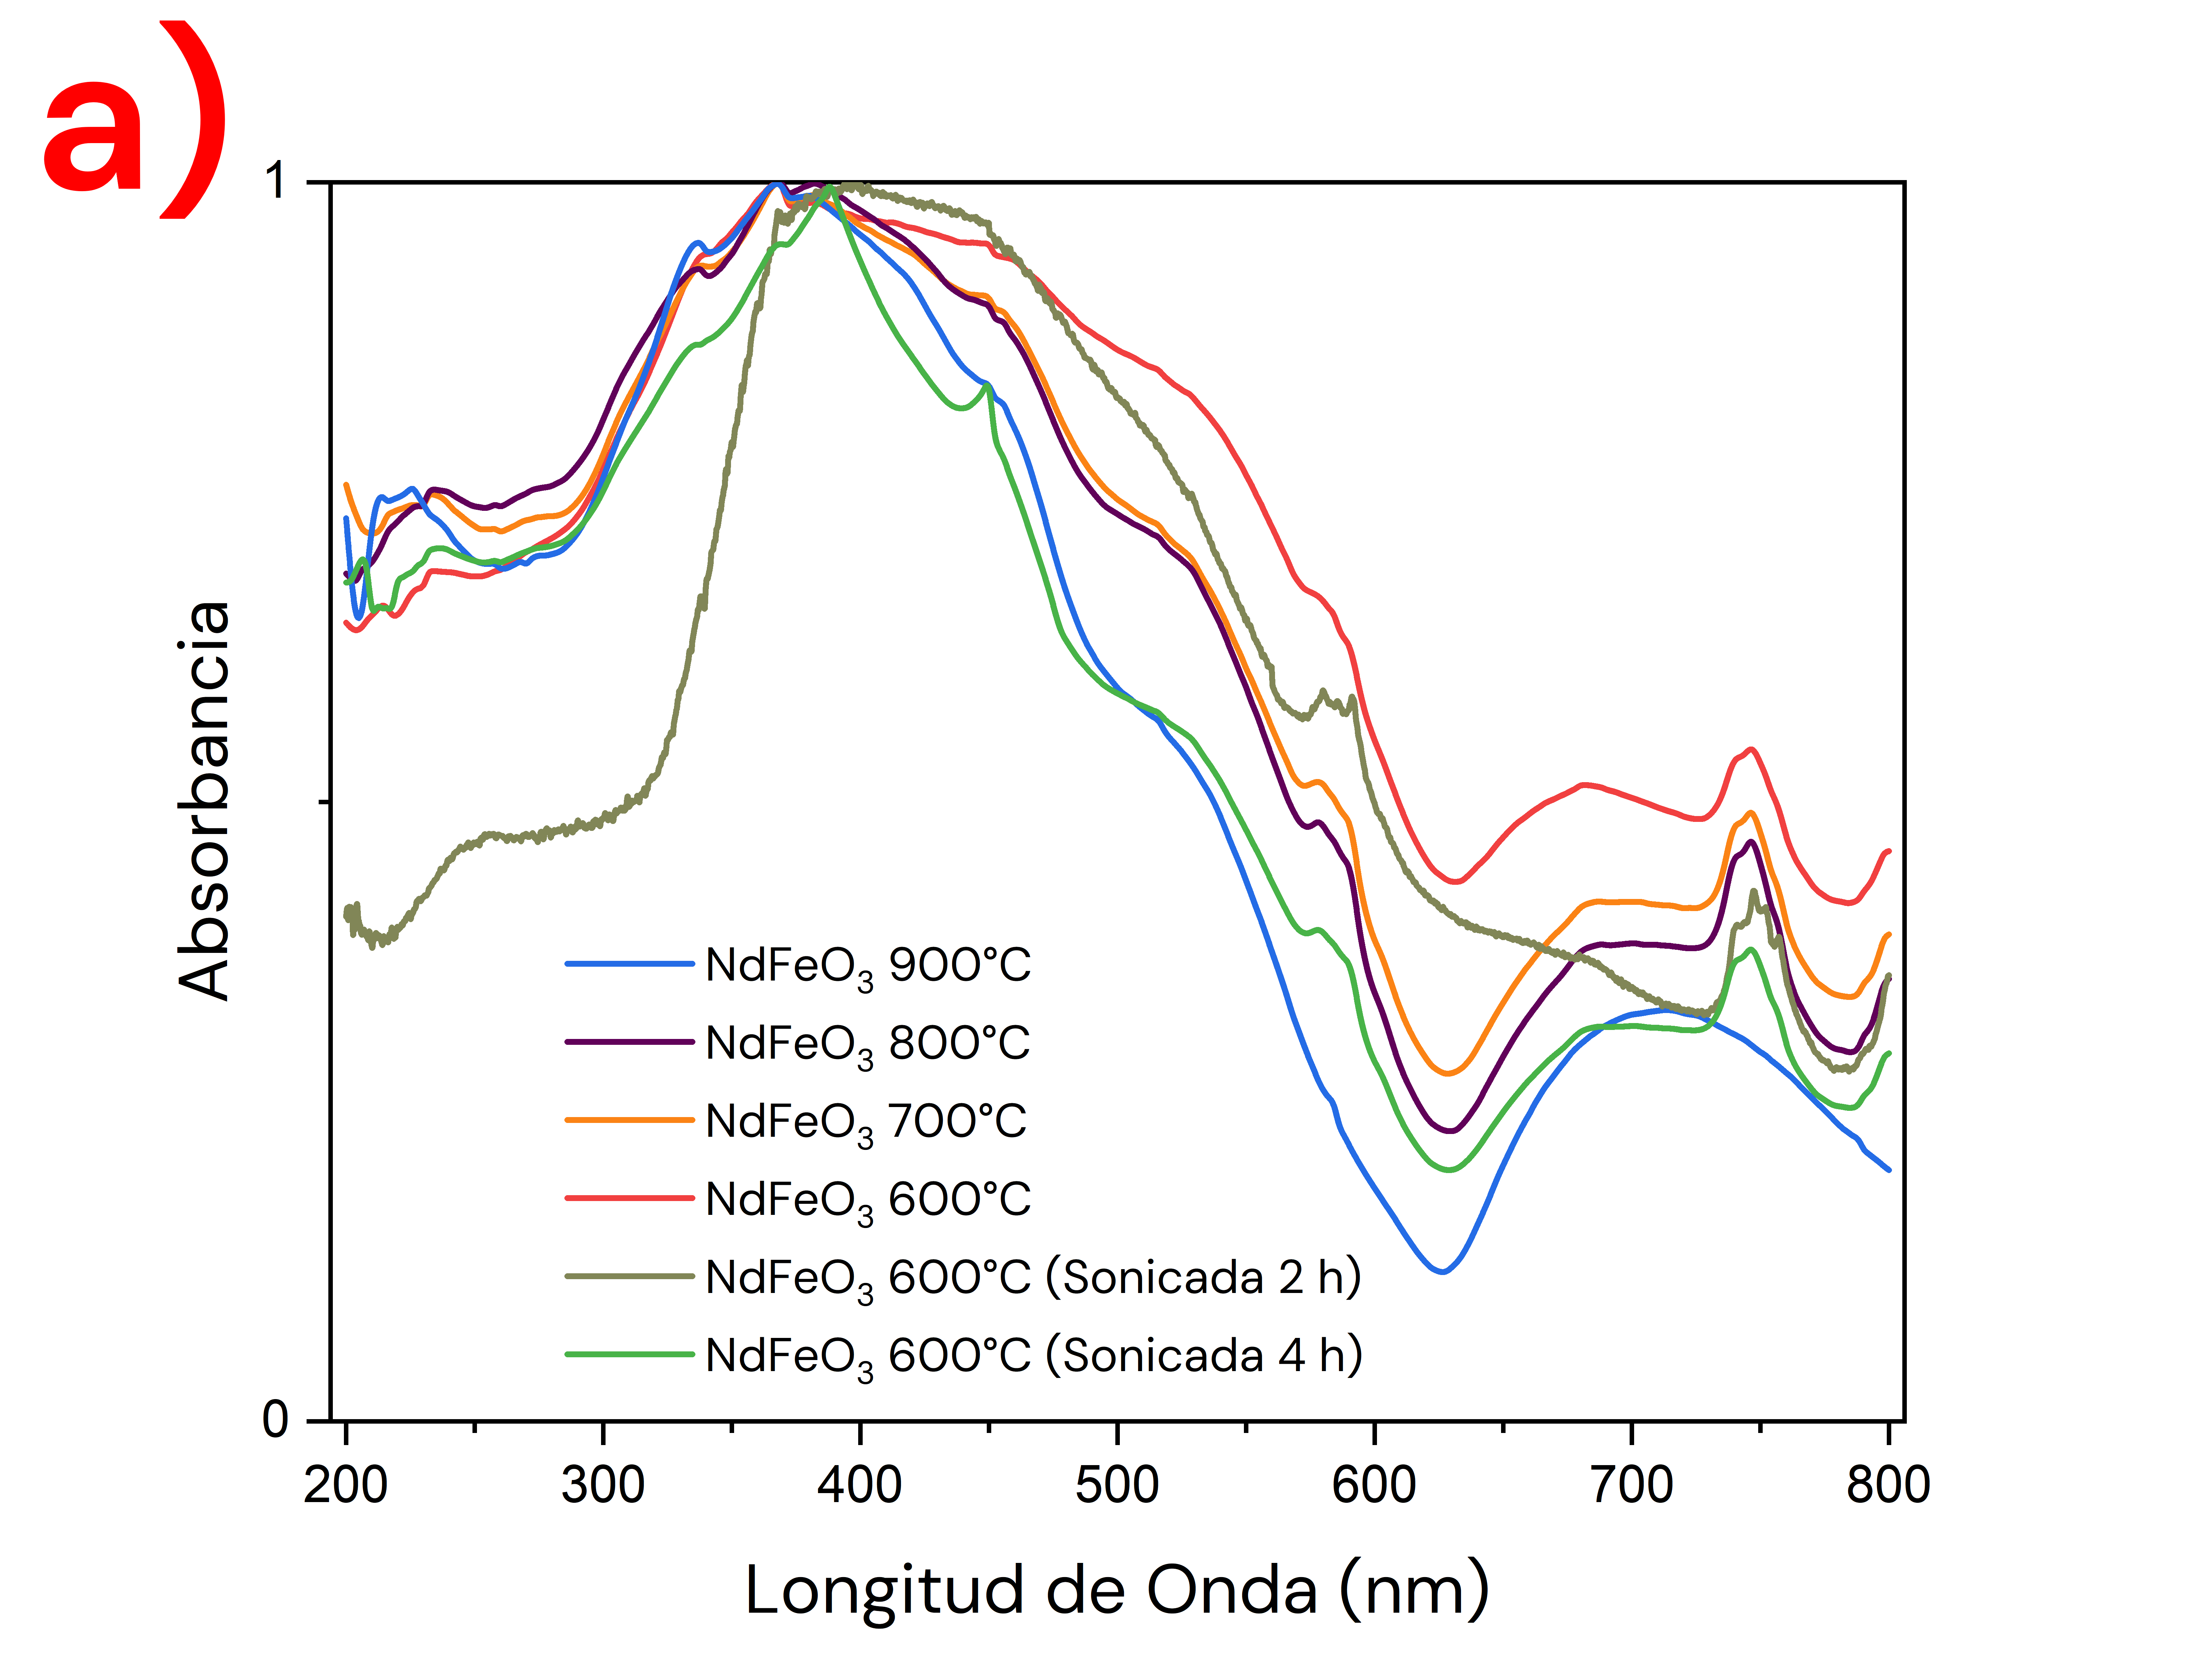
\includegraphics[width=0.7\textwidth]{fig/absorbancianeod.png}
    \caption{Gráficas de la absorbancia contra la longitud de onda para las muestras de \neod{}.}
    \label{fig:absorbresneod}
\end{figure}
Utilizando el método Tauc descrito en la sección \ref{sec:metodotauc} se llegó a los \textit{band gaps} para cada muestra reportados en la tabla \ref{tabla:bandgapsneod}, los cuales se grafican en la figura \ref{fig:bandgapvTneod}.
\begin{table}[H]
    \centering
    \begin{tabular}{|c||c|c|}
        \hline
        Muestra & Temperatura de & \textit{Band Gap} \\
        & calcinación & (eV) \\
        \hline\hline
        \multirow{6}{*}{\rotatebox[origin=c]{90}{\neod{}}} & 600\gradoC{} & 1.84$\pm$0.003 \\
        \cline{2-3}
        & 600\gradoC{}, sonicada 2 h & 2.01$\pm$0.001 \\
        \cline{2-3}
        & 600\gradoC{}, sonicada 4 h & 2.13$\pm$0.009 \\
        \cline{2-3}
        & 700\gradoC{} & 2.05$\pm$0.004 \\
        \cline{2-3}
        & 800\gradoC{} & 2.08$\pm$0.005 \\
        \cline{2-3}
        & 900\gradoC{} & 2.29$\pm$0.004 \\
        \hline
    \end{tabular} 
    \caption{\textit{Band gaps} de las distintas muestras de \neod{} según su temperatura de calcinación.}
    \label{tabla:bandgapsneod}
\end{table}
\begin{figure}[H]
    \centering
    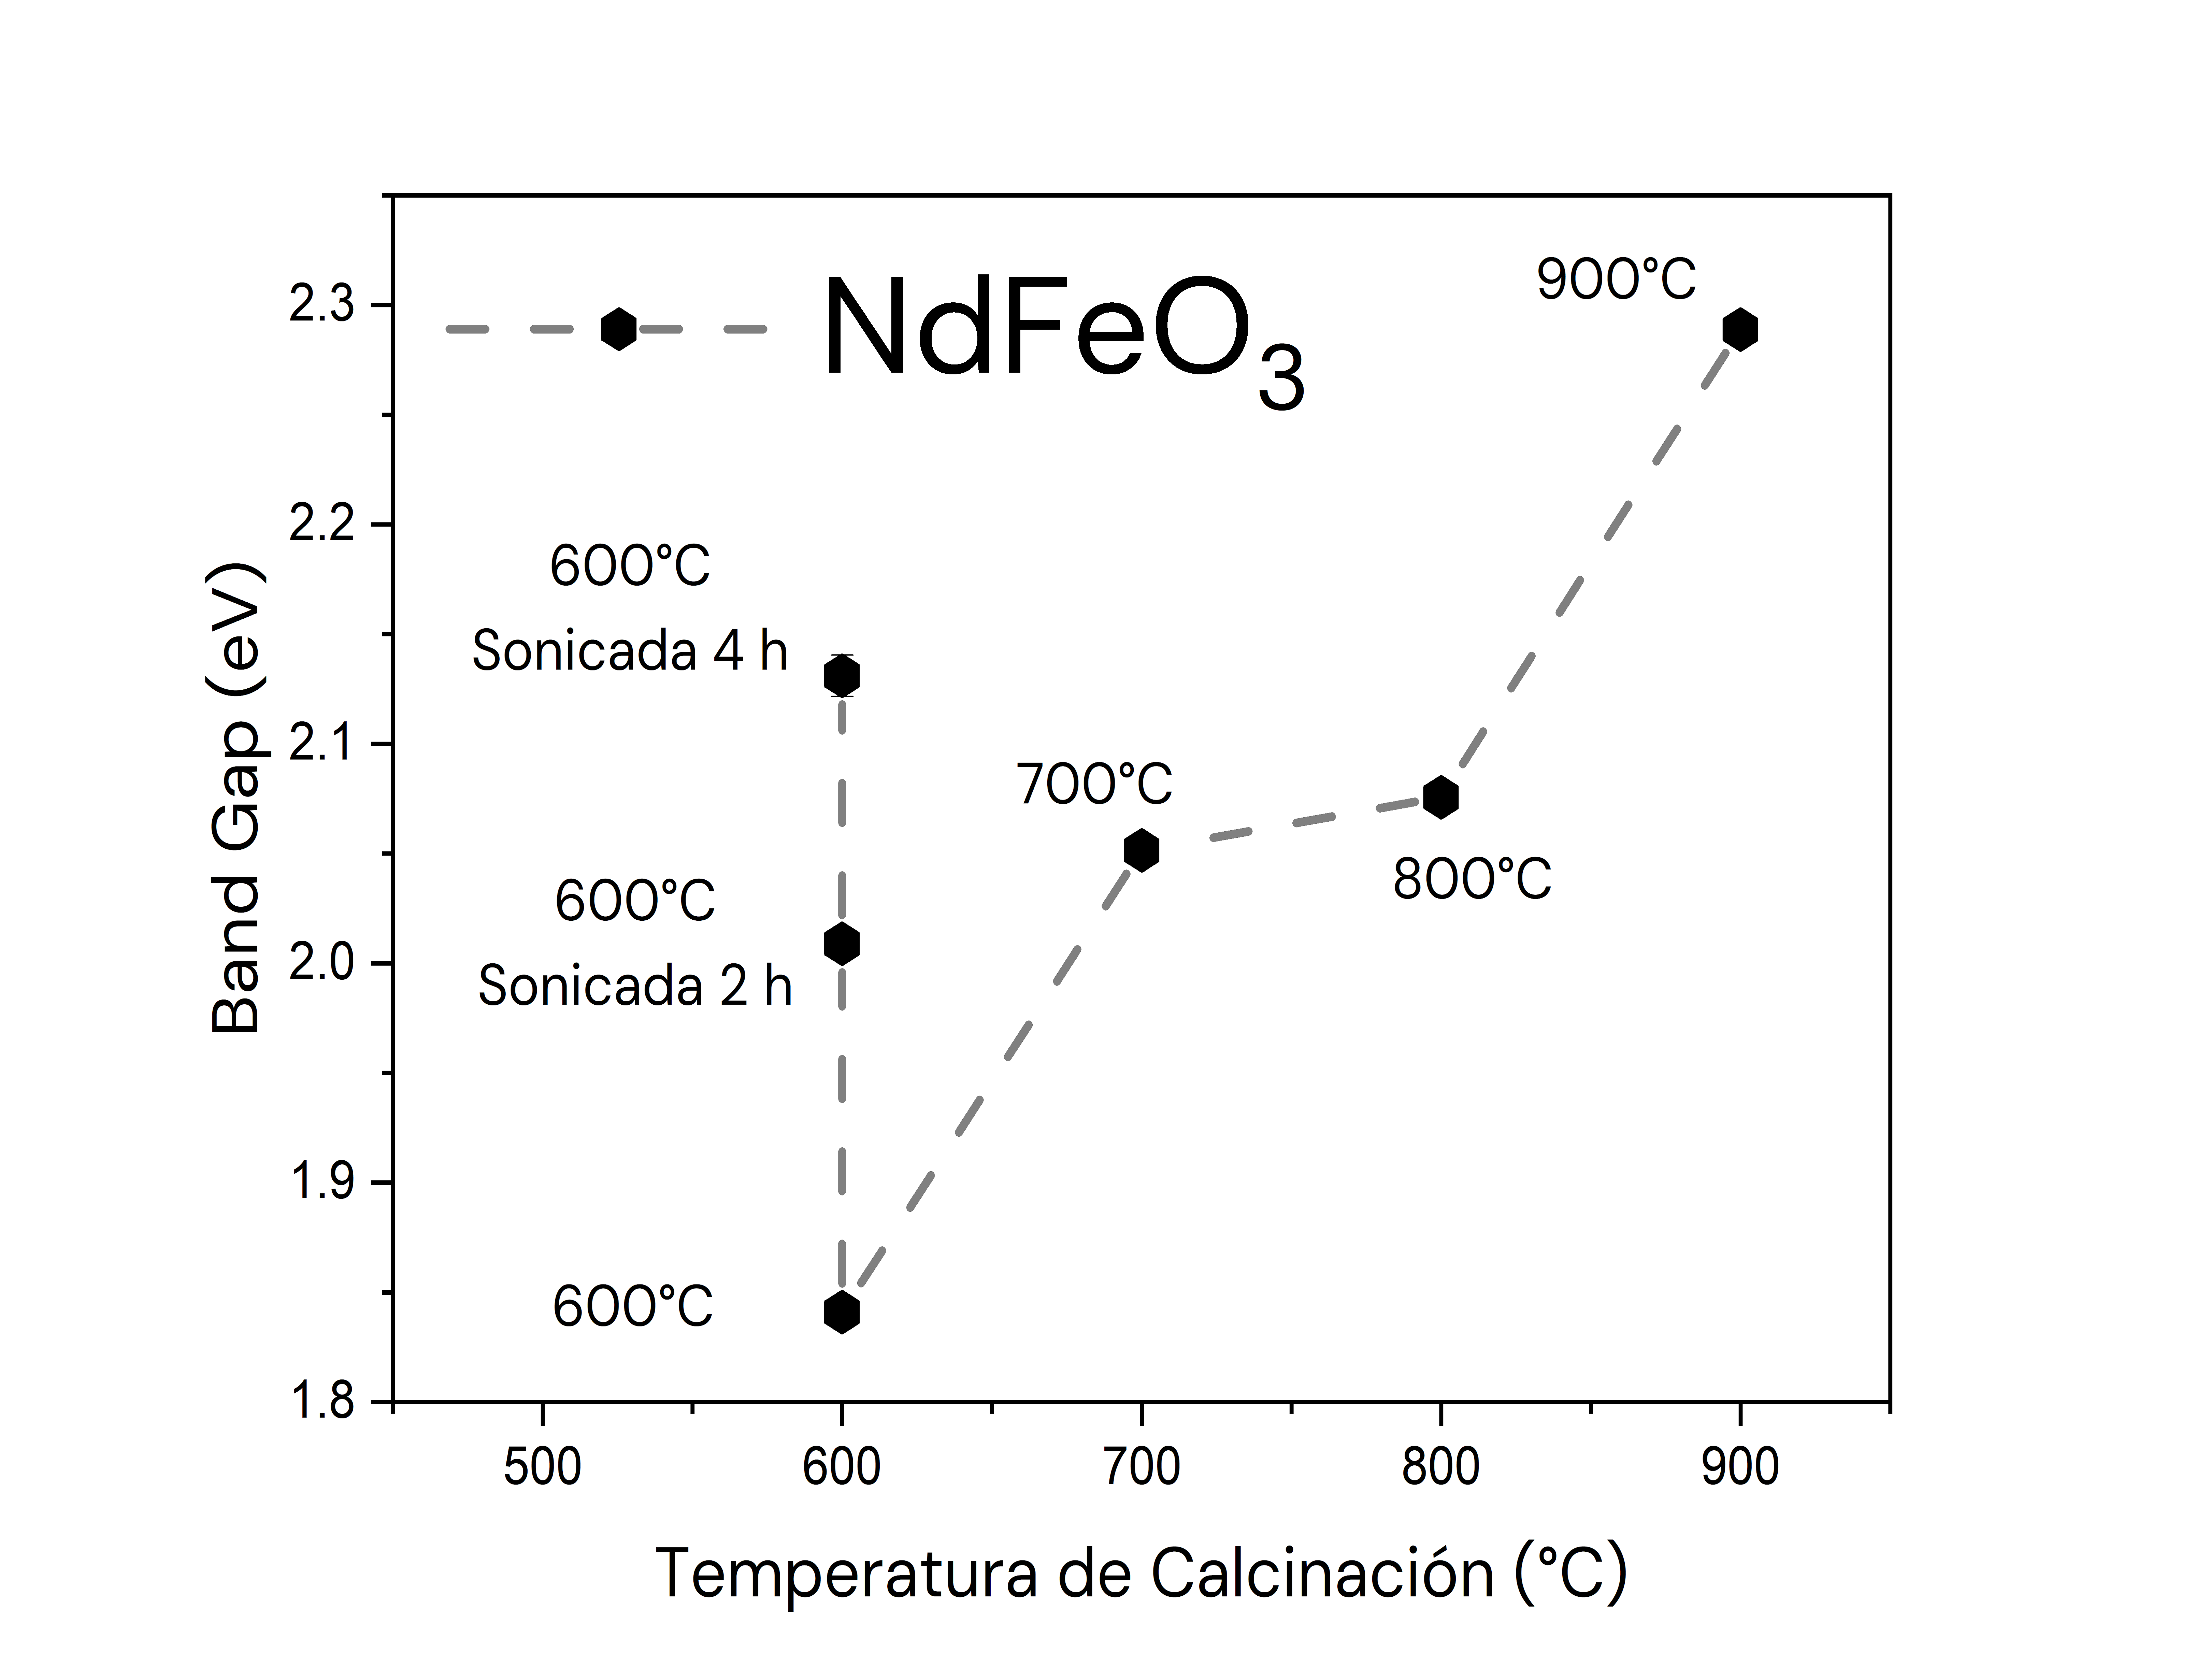
\includegraphics[width=0.7\textwidth]{fig/BGNdFeO3.png}
    \caption{Gráfica del \textit{band gap} de cada muestra de \neod{} según su temperatura de calcinación.}
    \label{fig:bandgapvTneod}
\end{figure}
Se observa que el \textit{band gap} aumenta con la temperatura y el tiempo de sonicación, teniendo un mínimo en la muestra calcinada a menor temperatura y sin sonicar.
\subsubsection{Magnetometría SQUID}
Se obtuvieron las siguientes curvas de $M$ vs $H$:
\begin{figure}[H]
    \centering
    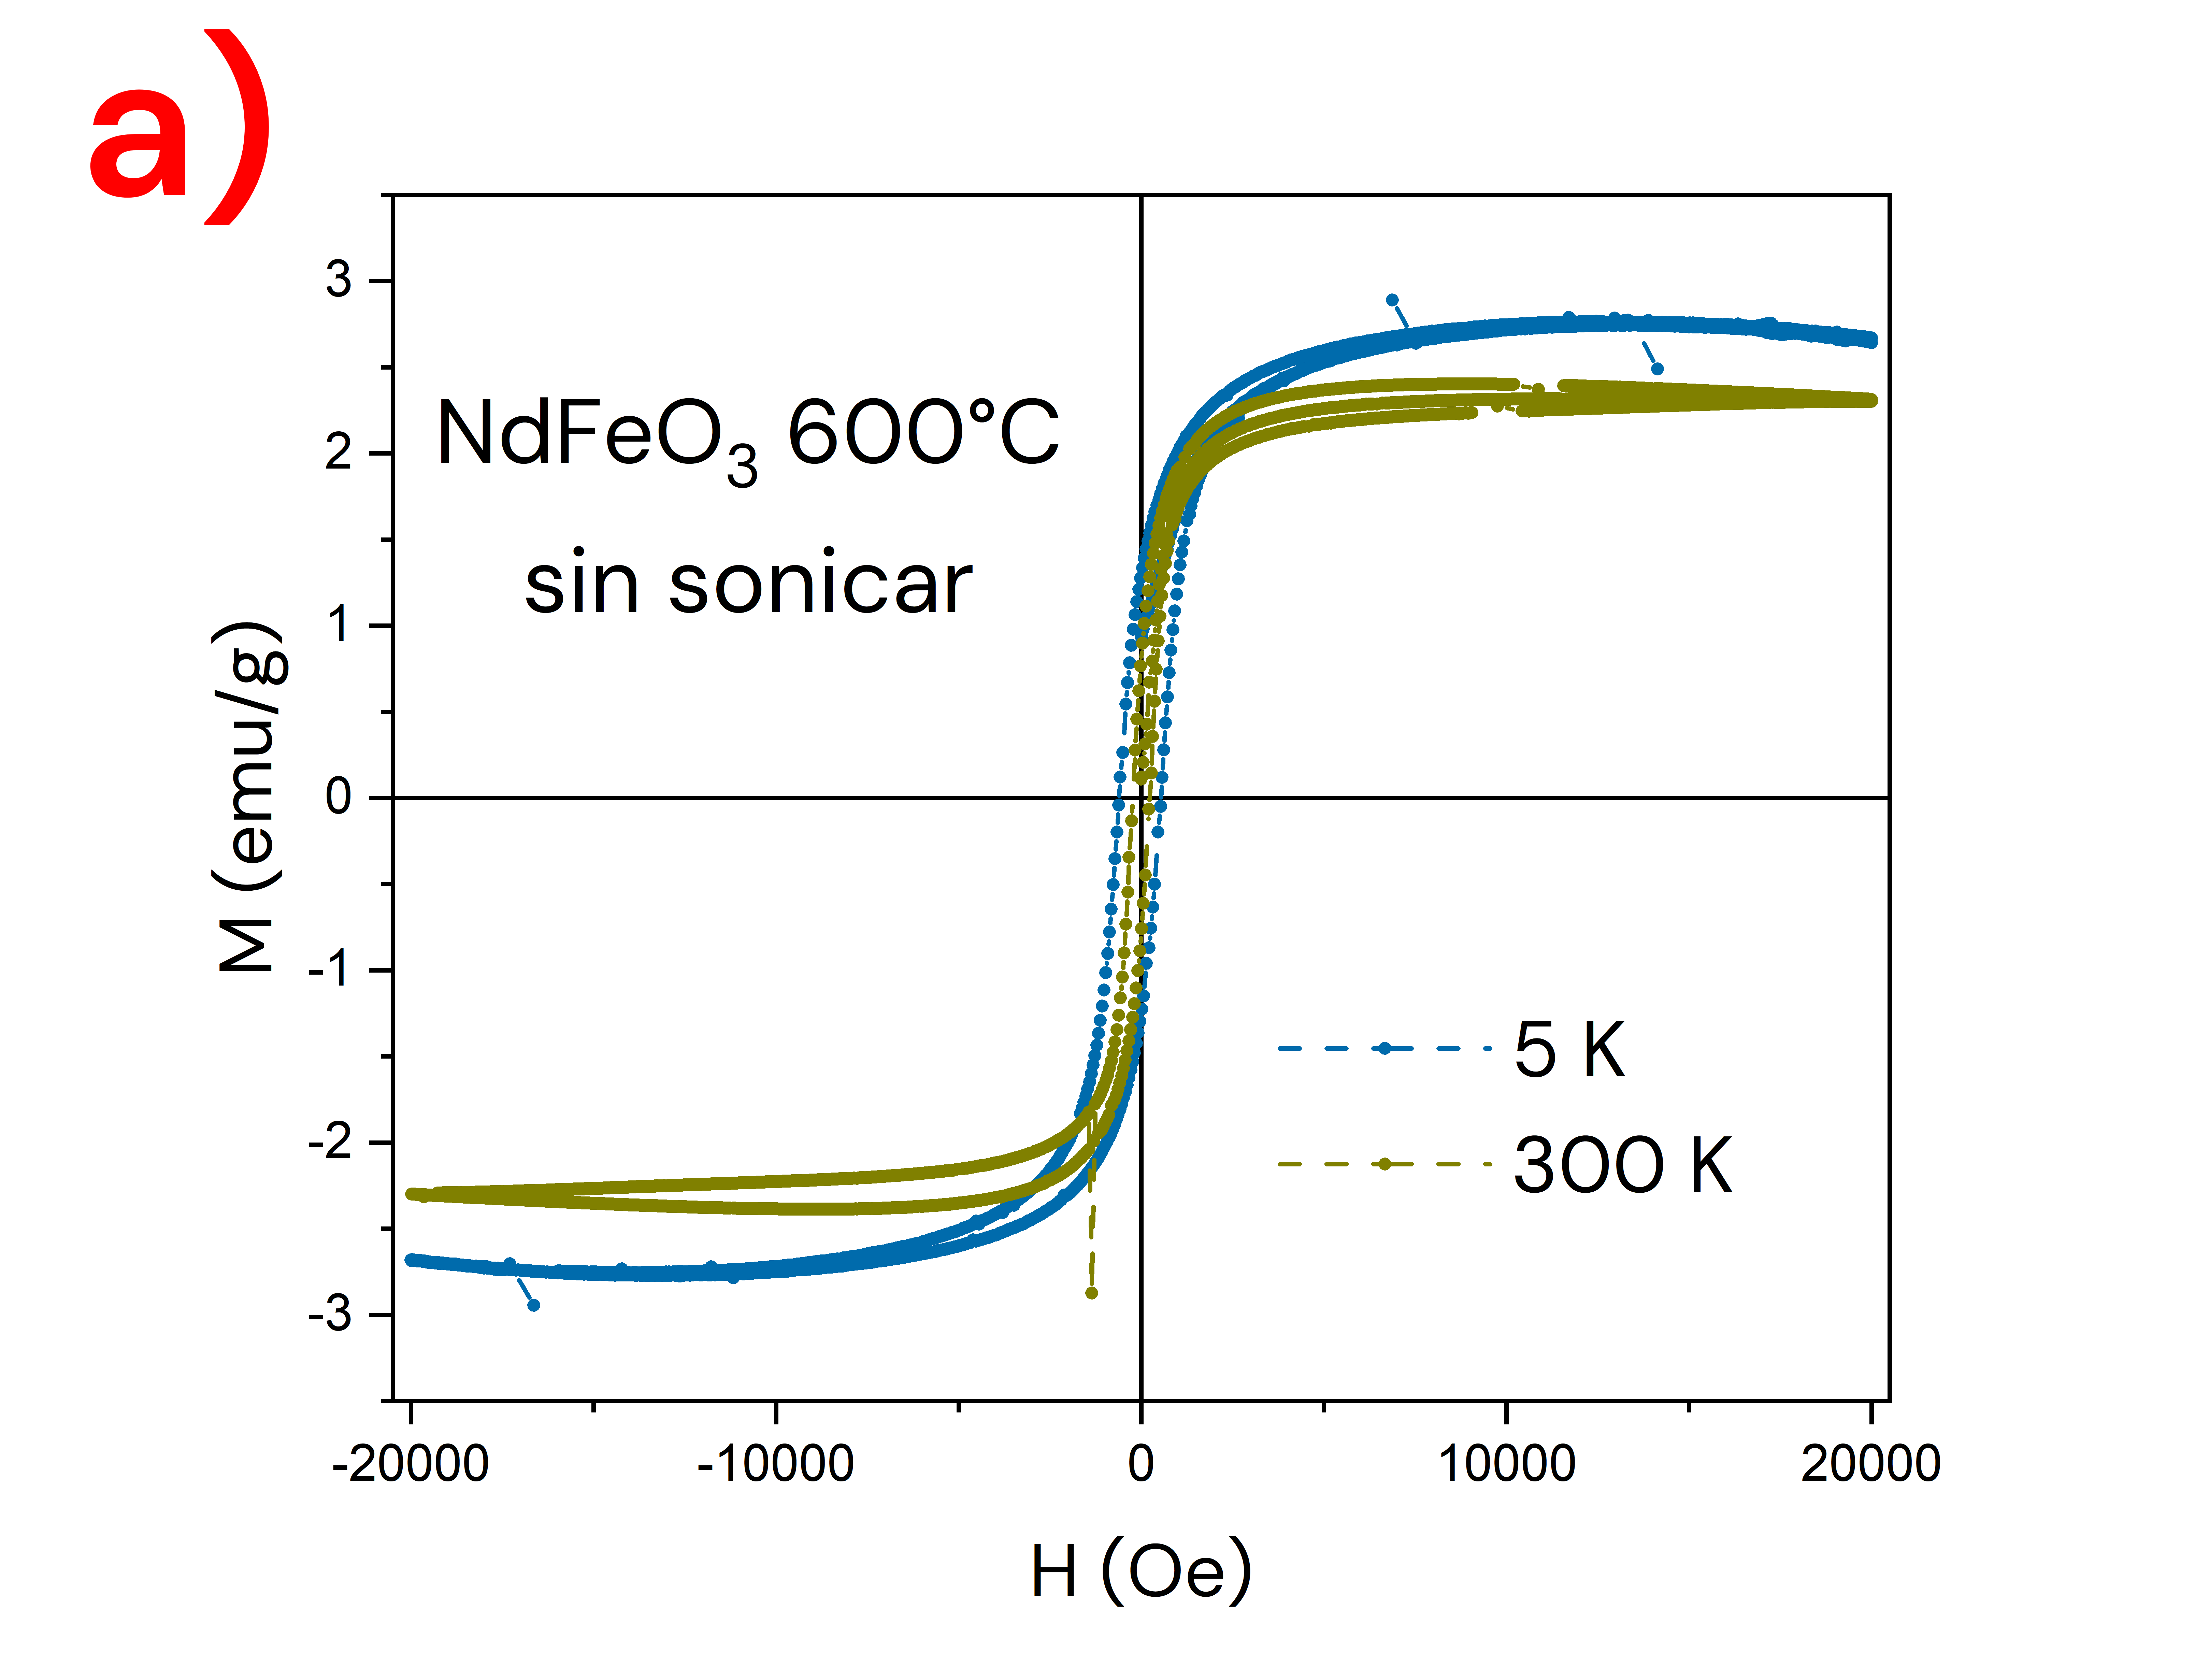
\includegraphics[width=0.45\textwidth]{fig/mvhNd.png}
    \quad
    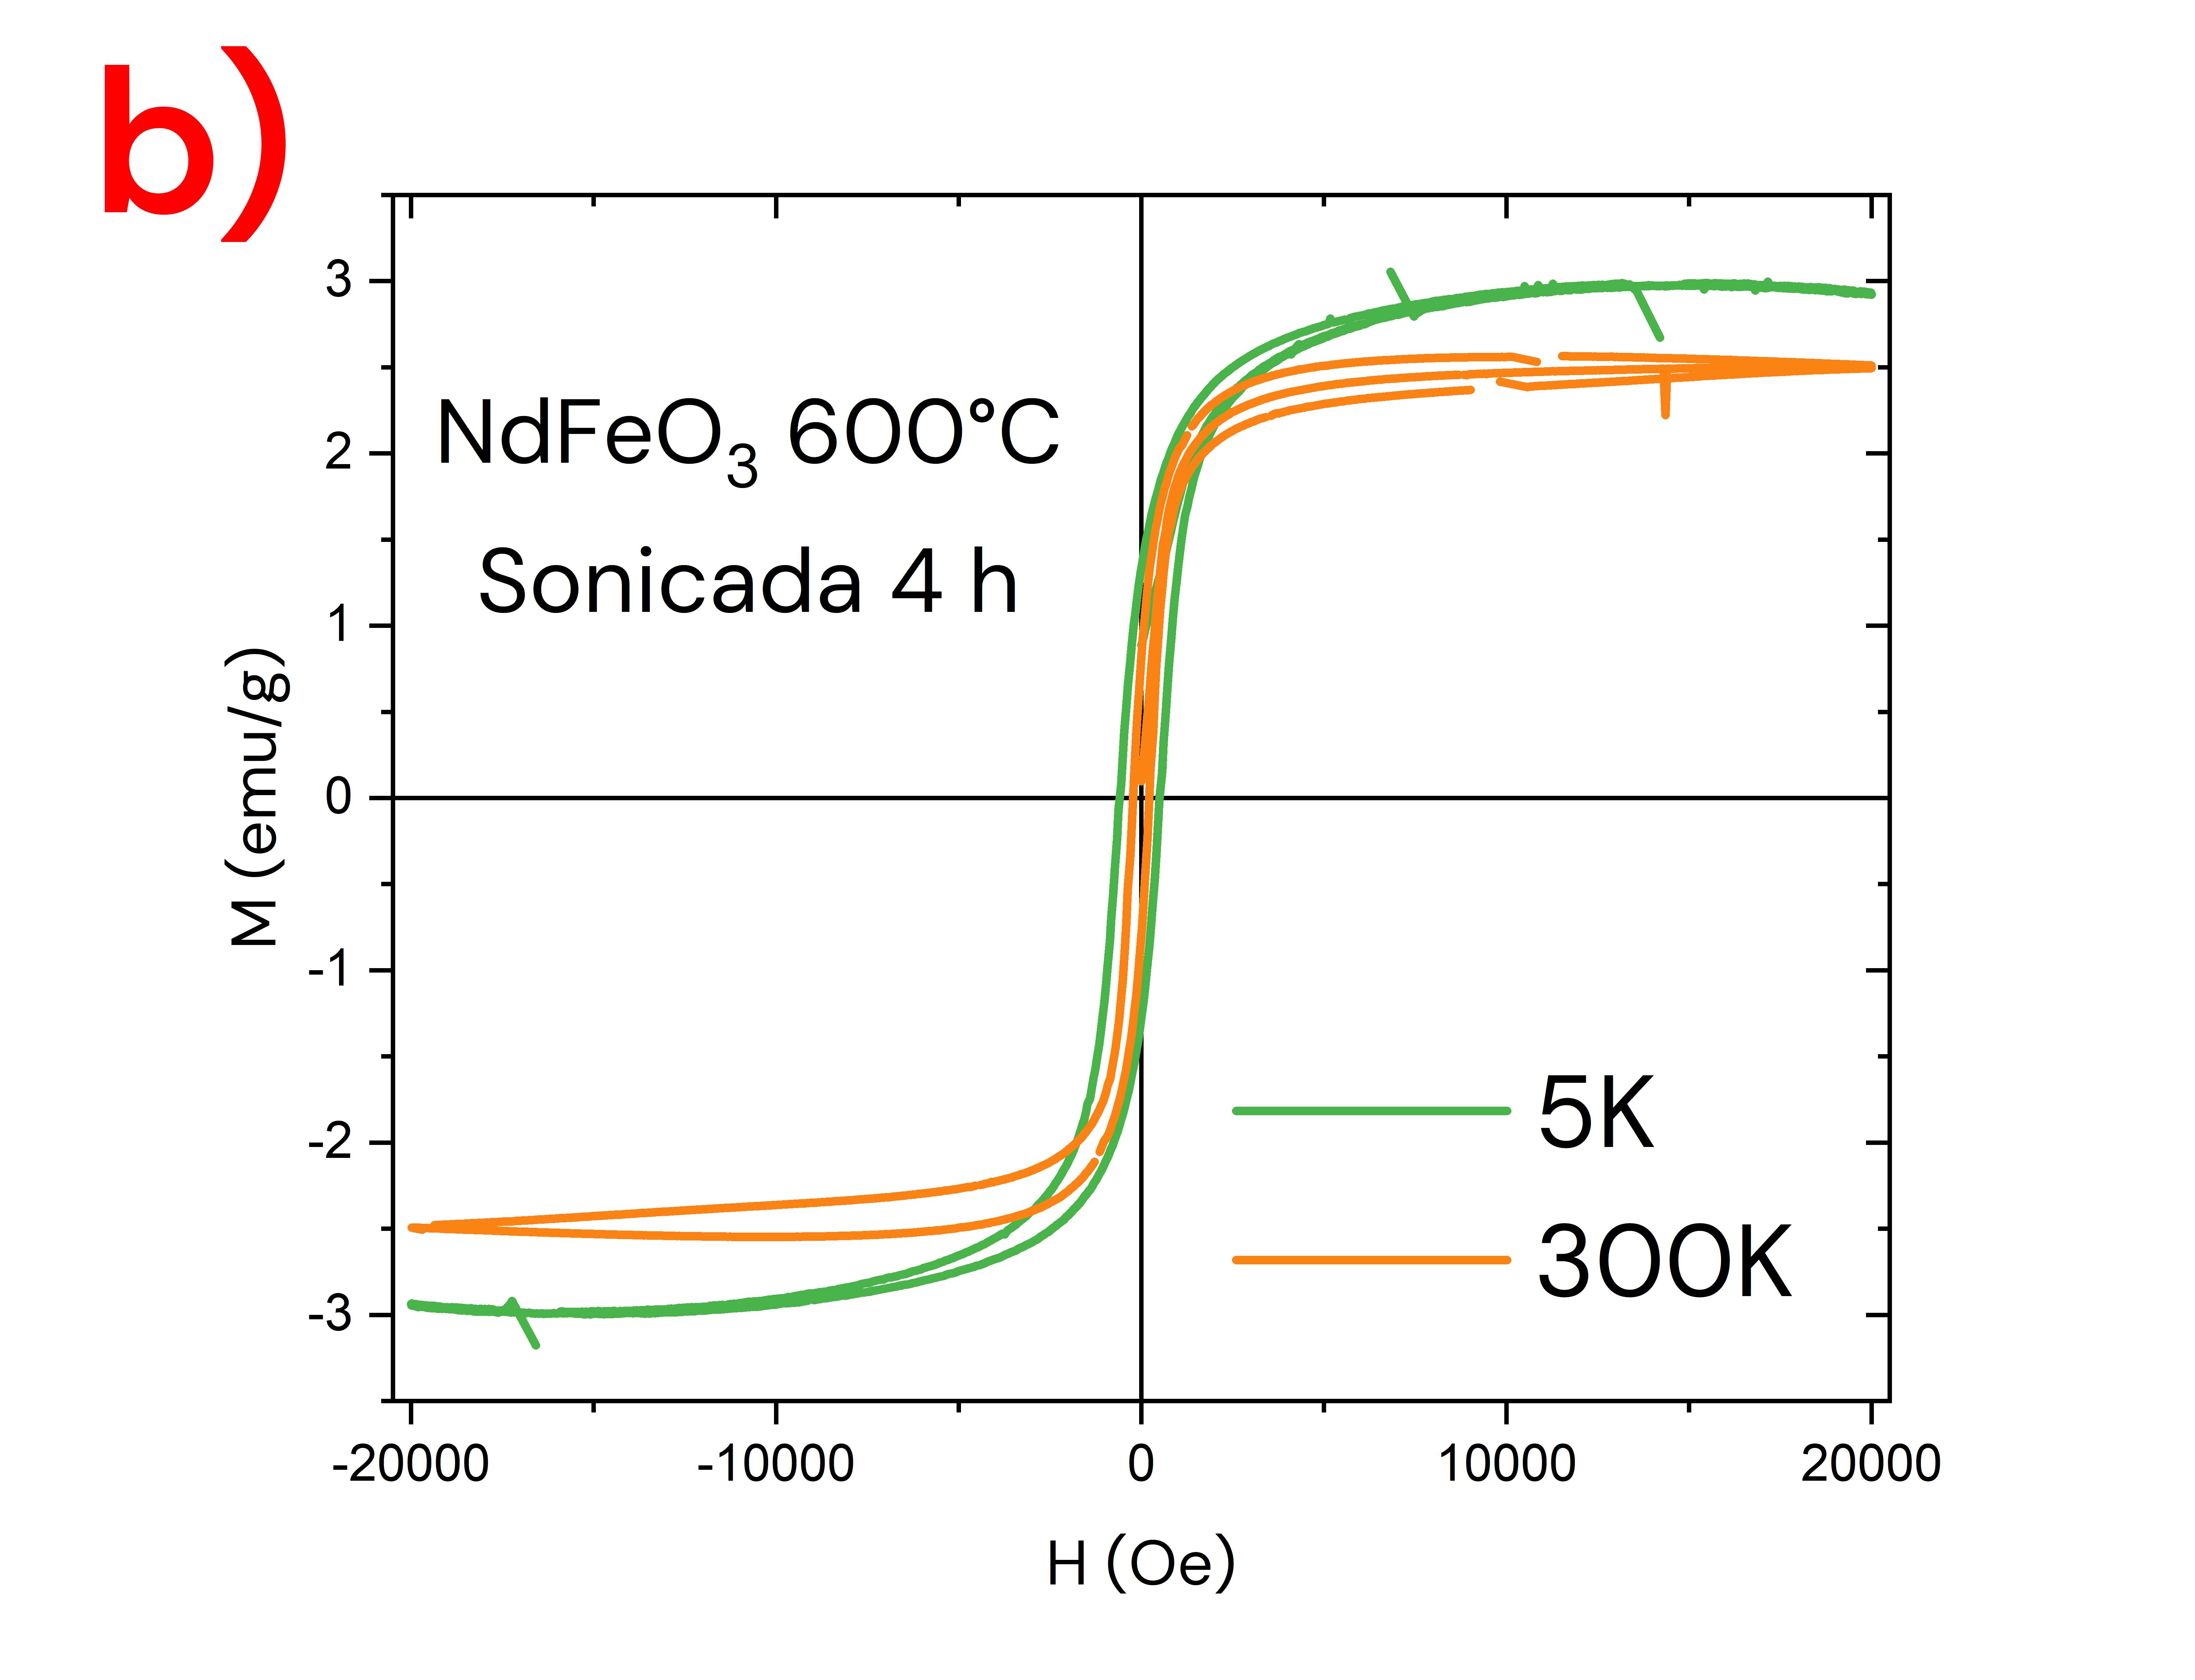
\includegraphics[width=0.45\textwidth]{fig/mvhNd-S.png}
    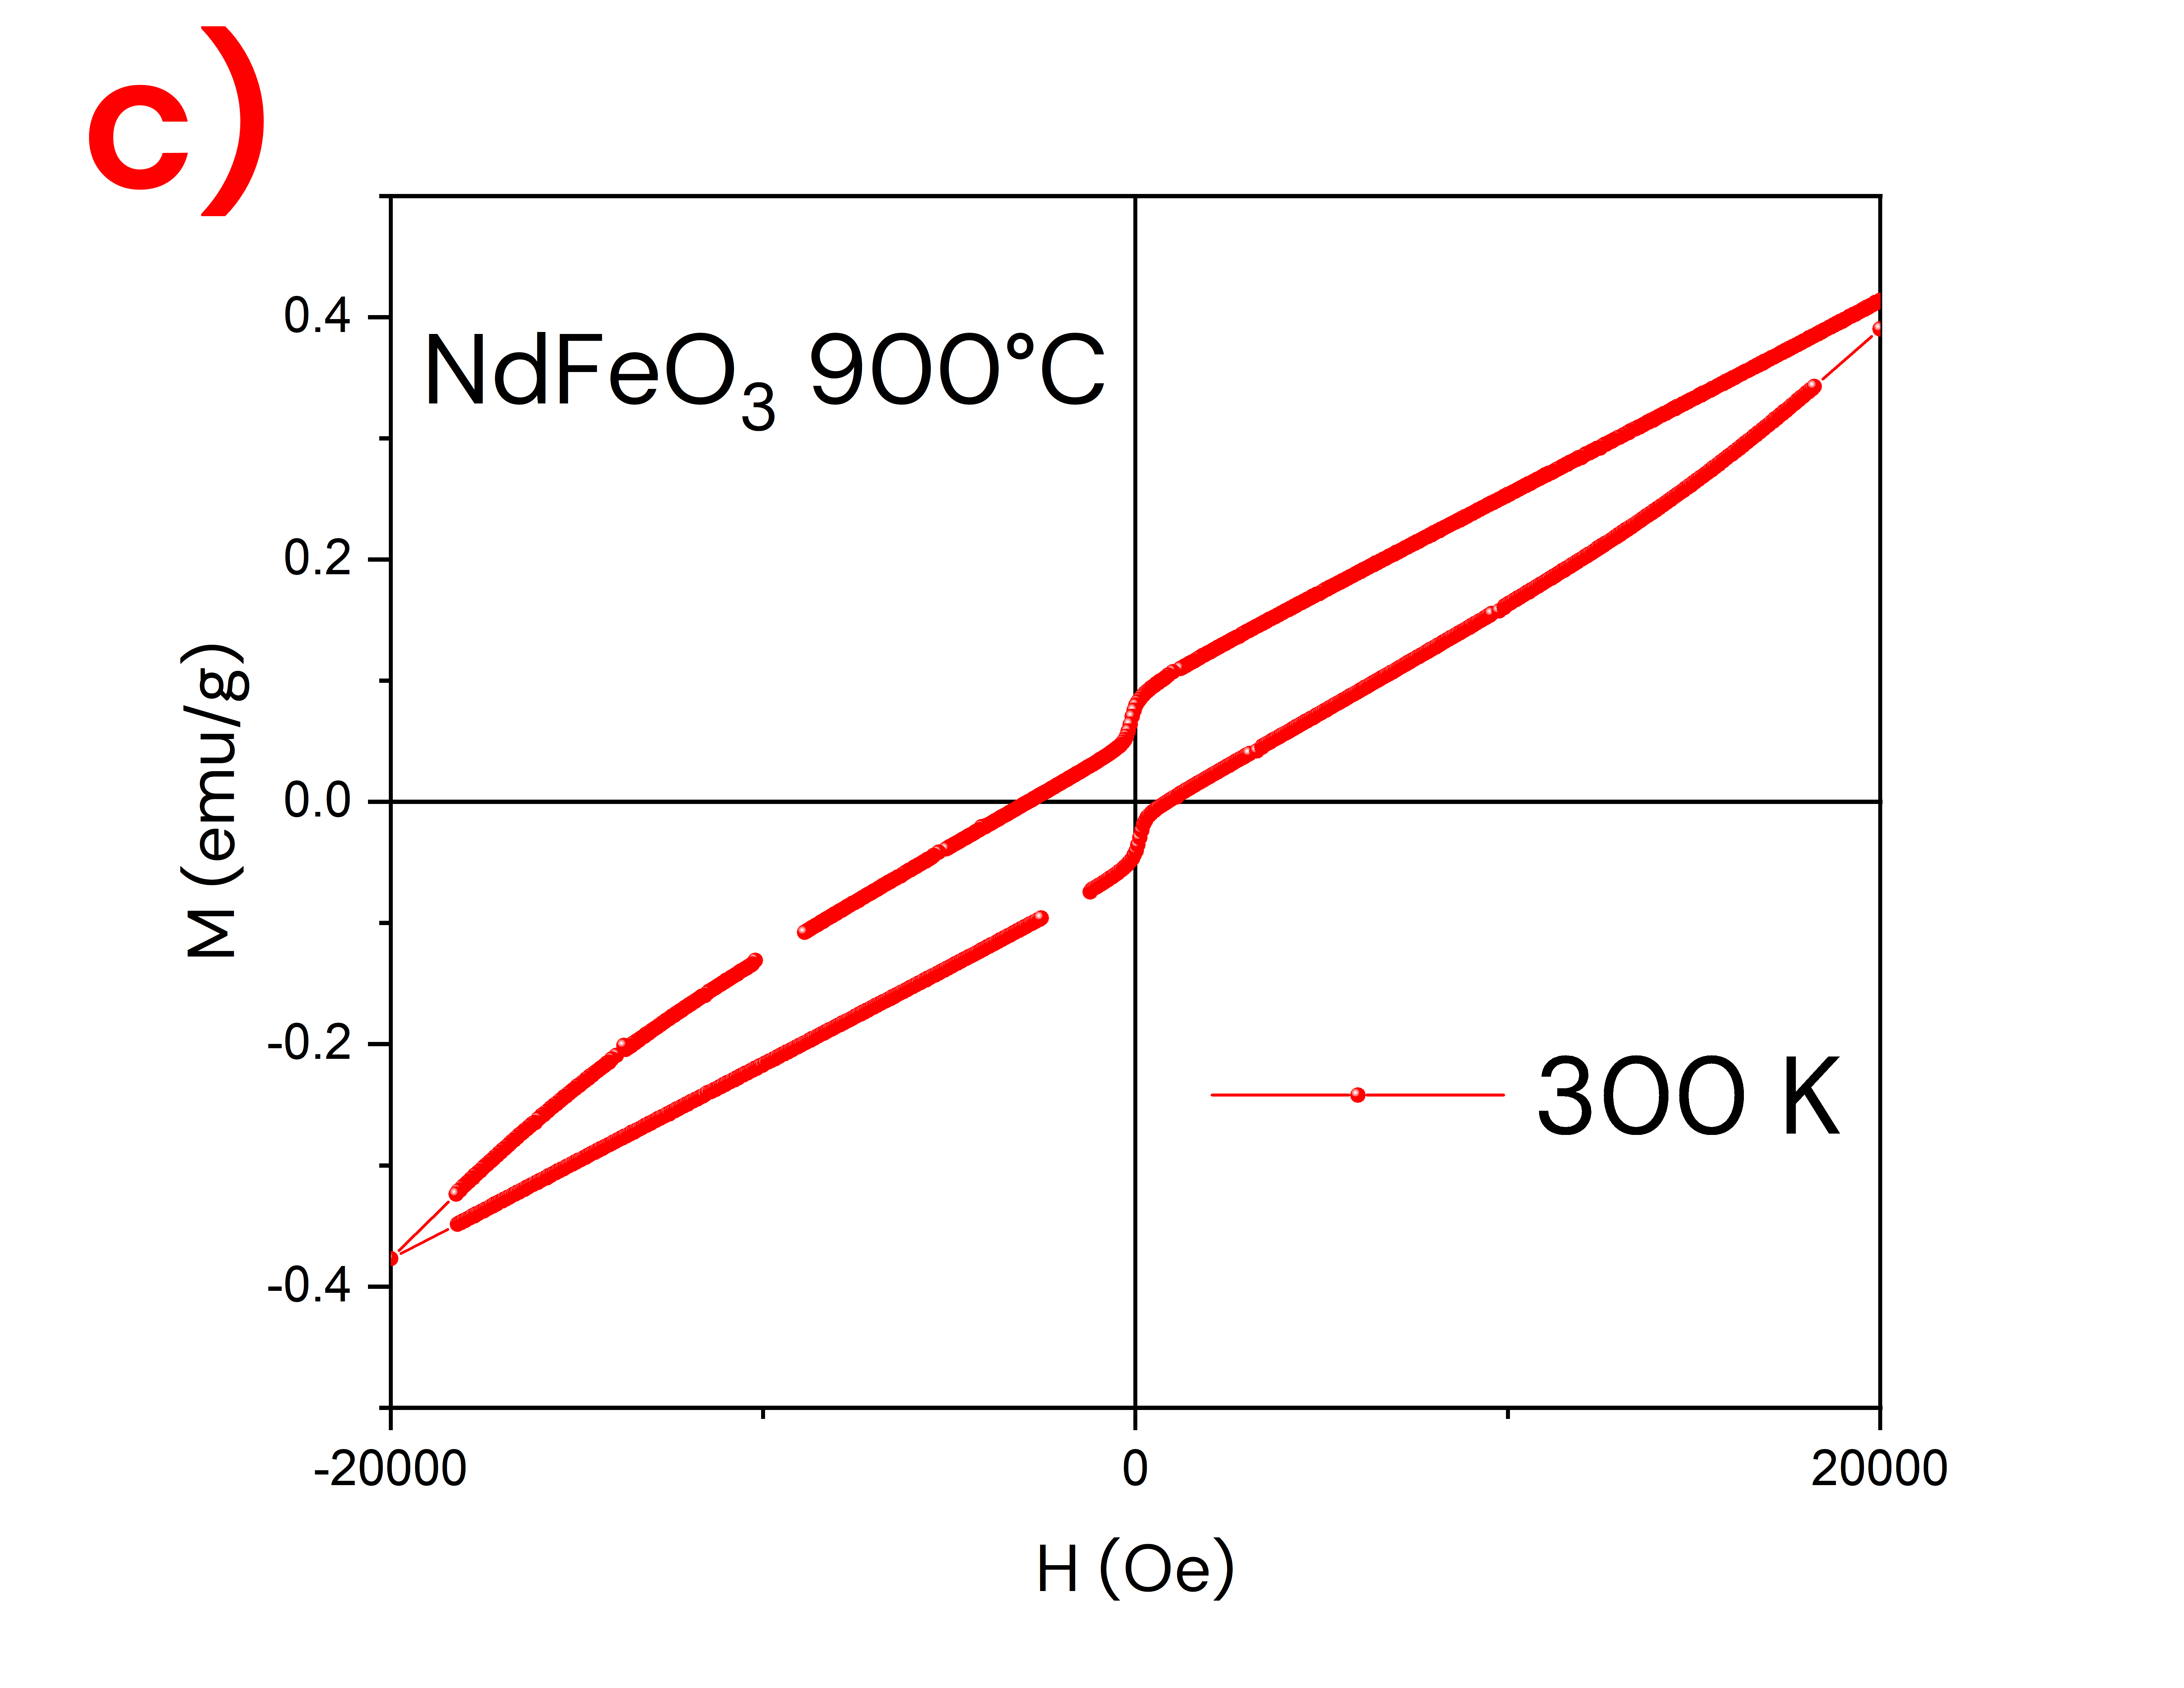
\includegraphics[width=0.45\textwidth]{fig/mvhNd900.png}
    \caption{Curvas $M$ contra $H$ para las muestras de \neod{}: a) calcinada a 600\gradoC{} sin sonicar, b) calcinada a 600\gradoC{} sonicada y c) calcinada a 900\gradoC{}.}
    \label{fig:mvhNd}
\end{figure}
No se observa un cambio significativo con la sonicación, sin embargo, el comportamiento de la muestra es totalmente distinto según su temperatura de calcinación.

Las muestras calcinadas a 600\gradoC{} muestran un comportamiento ferromagnético muy suave a temperatura ambiente, con $H_c$ y $M_r\approx0$, el cual, como es de esperarse para este tipo de material, tiende a ferromagnético al bajar la temperatura. Por otro lado, la muestra calcinada a 900\gradoC{} muestra un comportamiento ferromagnético débil, lo cual es consistente con la estructura antiferromagnética reportada en \cite{Wang2019}.

A continuación se reportan los valores obtenidos para $M_r$, $M_s$ y $H_c$.
\begin{table}[H]
    \centering
    \begin{tabular}{|c||c|c|c|}
        \hline 
        Muestra & $M_s$ (emu/g) & $M_r$ (emu/g) & $H_c$ (Oe) \\
        \hline
        \hline
        \multicolumn{4}{|c|}{$T=5$ K} \\
        \hline
        \neod{} (600\gradoC{}) sin sonicar & 2.83$\pm$0.006 & 1.74$\pm$0.024 & 523.71$\pm$23.818 \\
        \hline
        \neod{} (600\gradoC{}) sonicada 4 h & 2.63$\pm$0.011 & 1.44$\pm$0.032 & 219.61$\pm$17.736 \\
        \hline
        \multicolumn{4}{|c|}{$T=300$ K} \\
        \hline 
        Muestra & $M_s$ (emu/g) & $M_r$ (emu/g) & $H_c$ (Oe) \\
        \hline
        \hline
        \neod{} (600\gradoC{}) sin sonicar & 2.18$\pm$0.001 & 0.83$\pm$0.012 & 163.64$\pm$74.669 \\
        \hline
        \neod{} (600\gradoC{}) sonicada 4 h & 2.34$\pm$0.001 & 0.92$\pm$0.039 & 153.87$\pm$28.621 \\
        \hline
        \neod{} (900\gradoC{}) & 0.09$\pm$0.002 & 0.08$\pm$0.001 & 2832.19$\pm$53.892 \\
        \hline
        \end{tabular} 
    \caption{Valores de $M_s$, $M_r$ y $H_c$ obtenidos para las muestras de \neod{}.}
    \label{tabla:resmvshneod}
\end{table}
Por otra parte, se obtuvieron las siguientes curvas $M$ vs $T$ y $\chi$ vs $T$:
\begin{figure}[H]
    \centering
    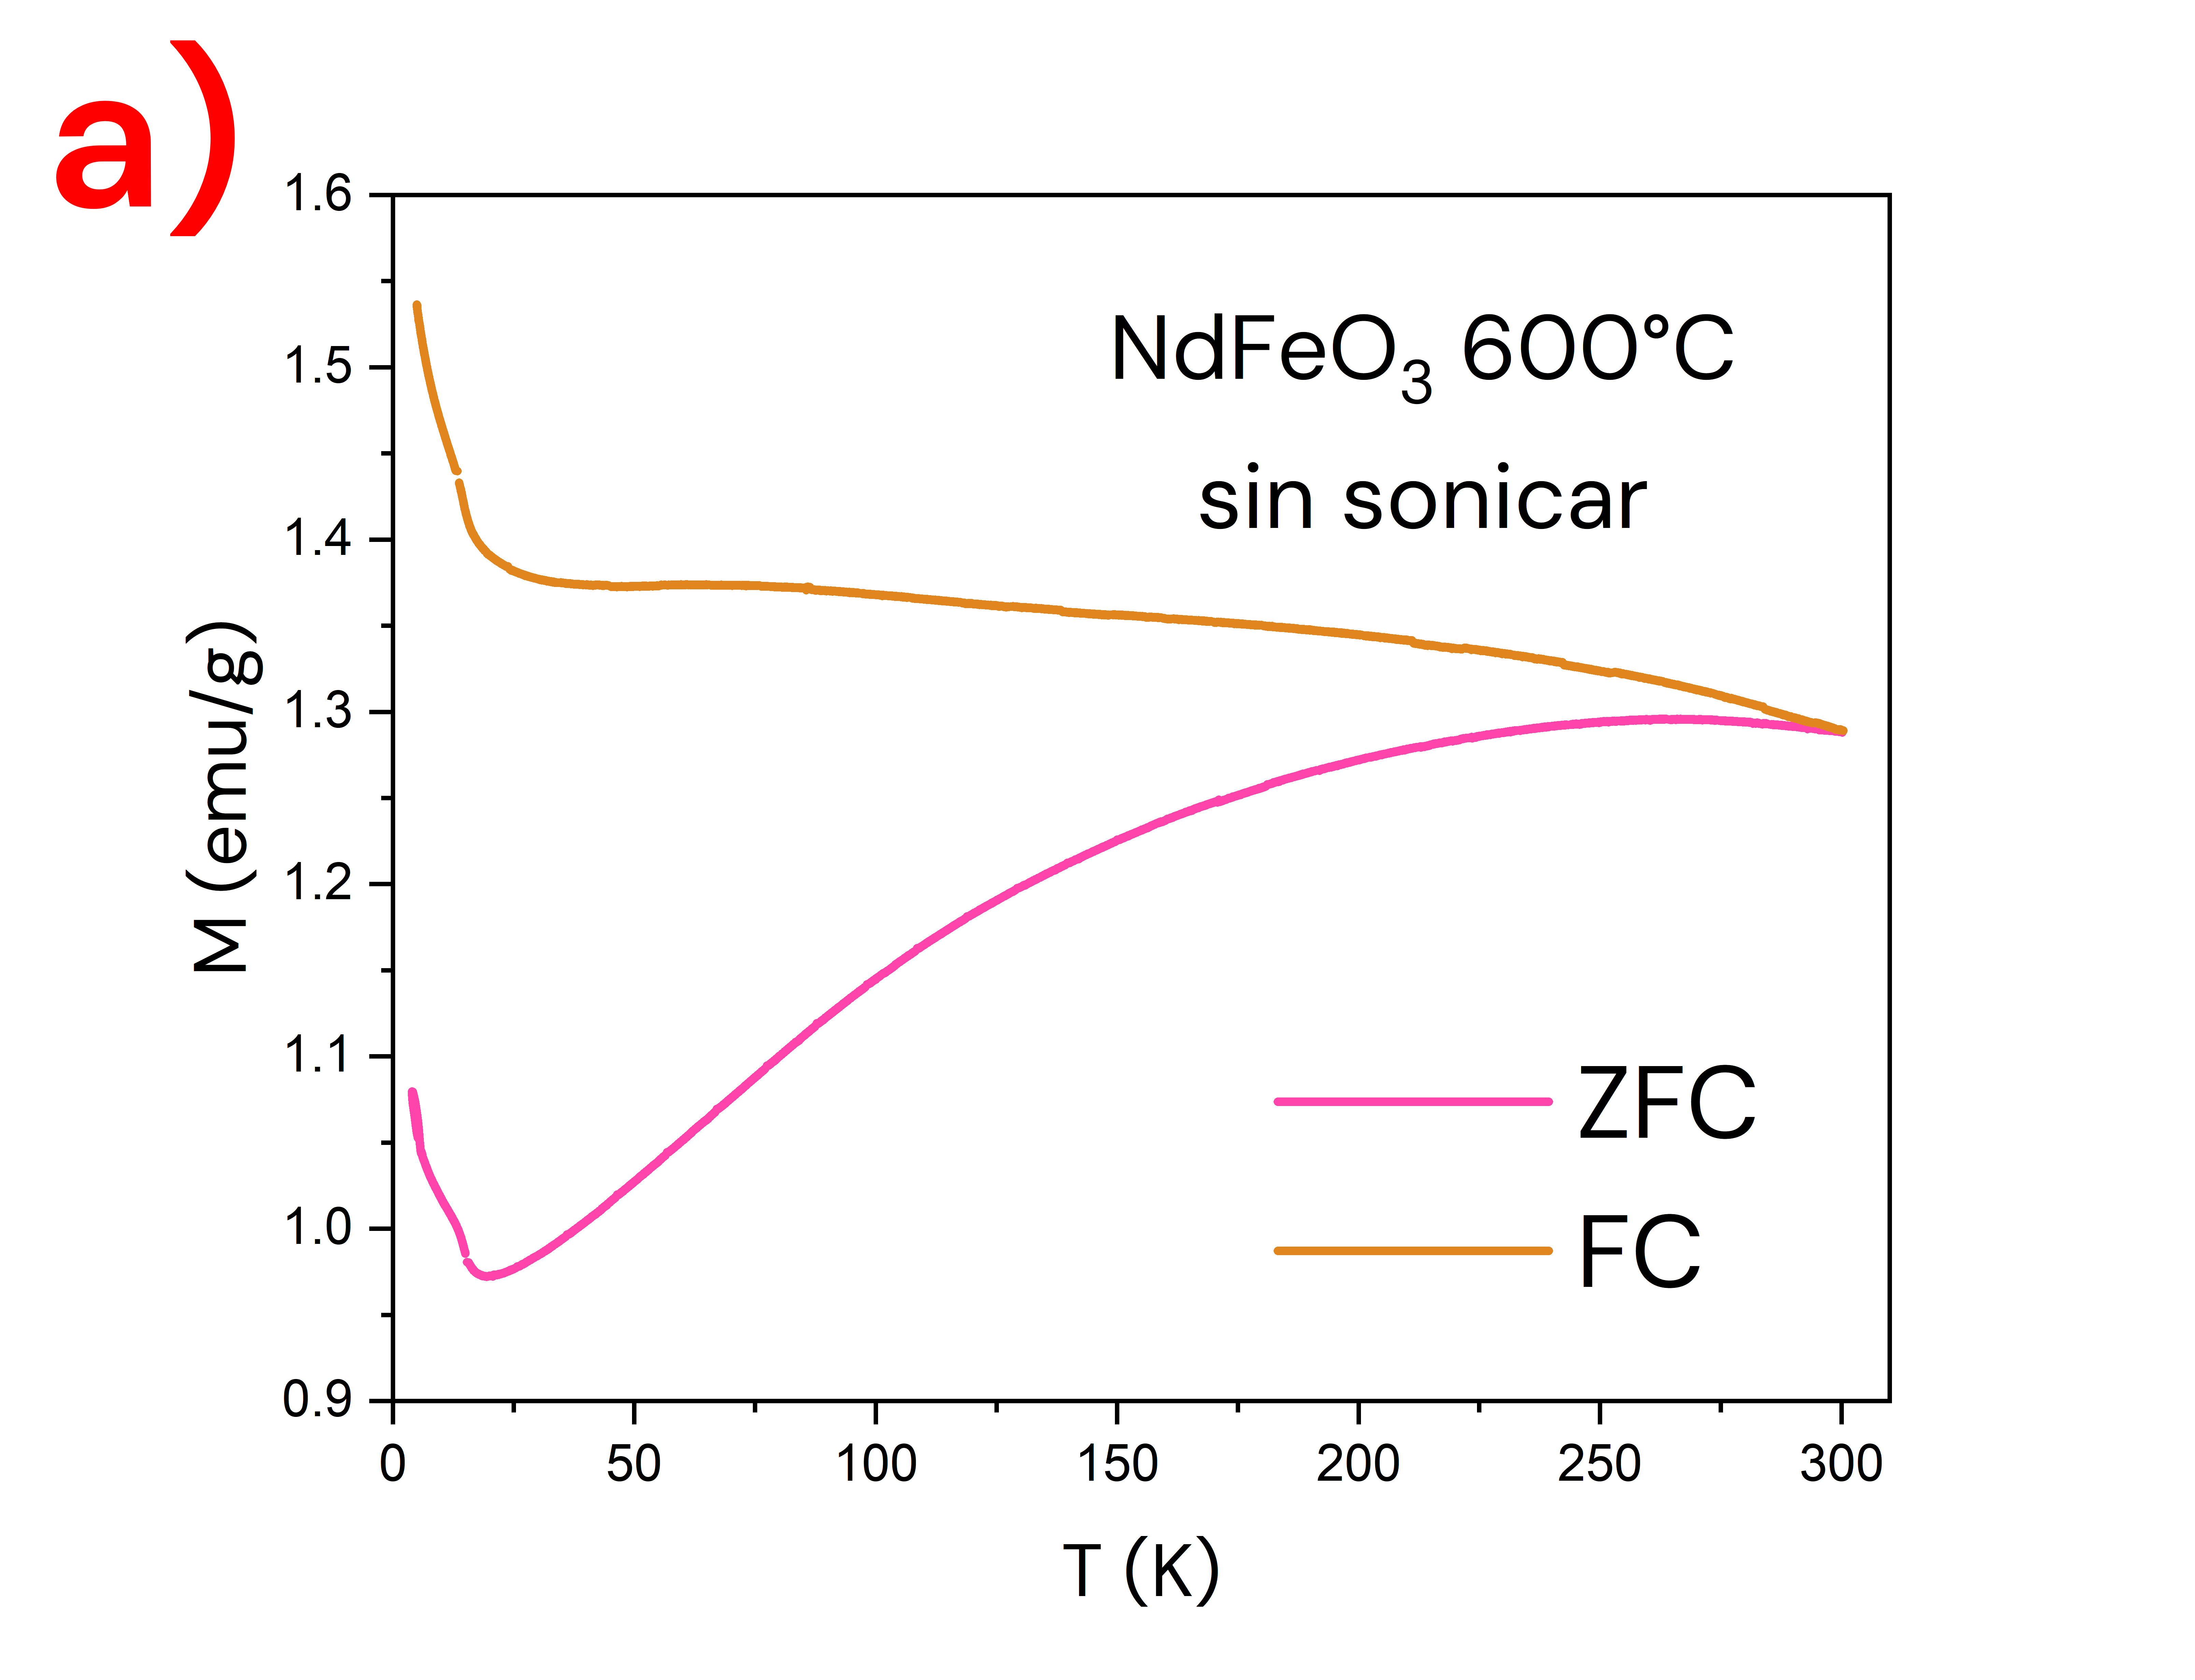
\includegraphics[width=0.45\textwidth]{fig/MvTNd.png}
    \quad
    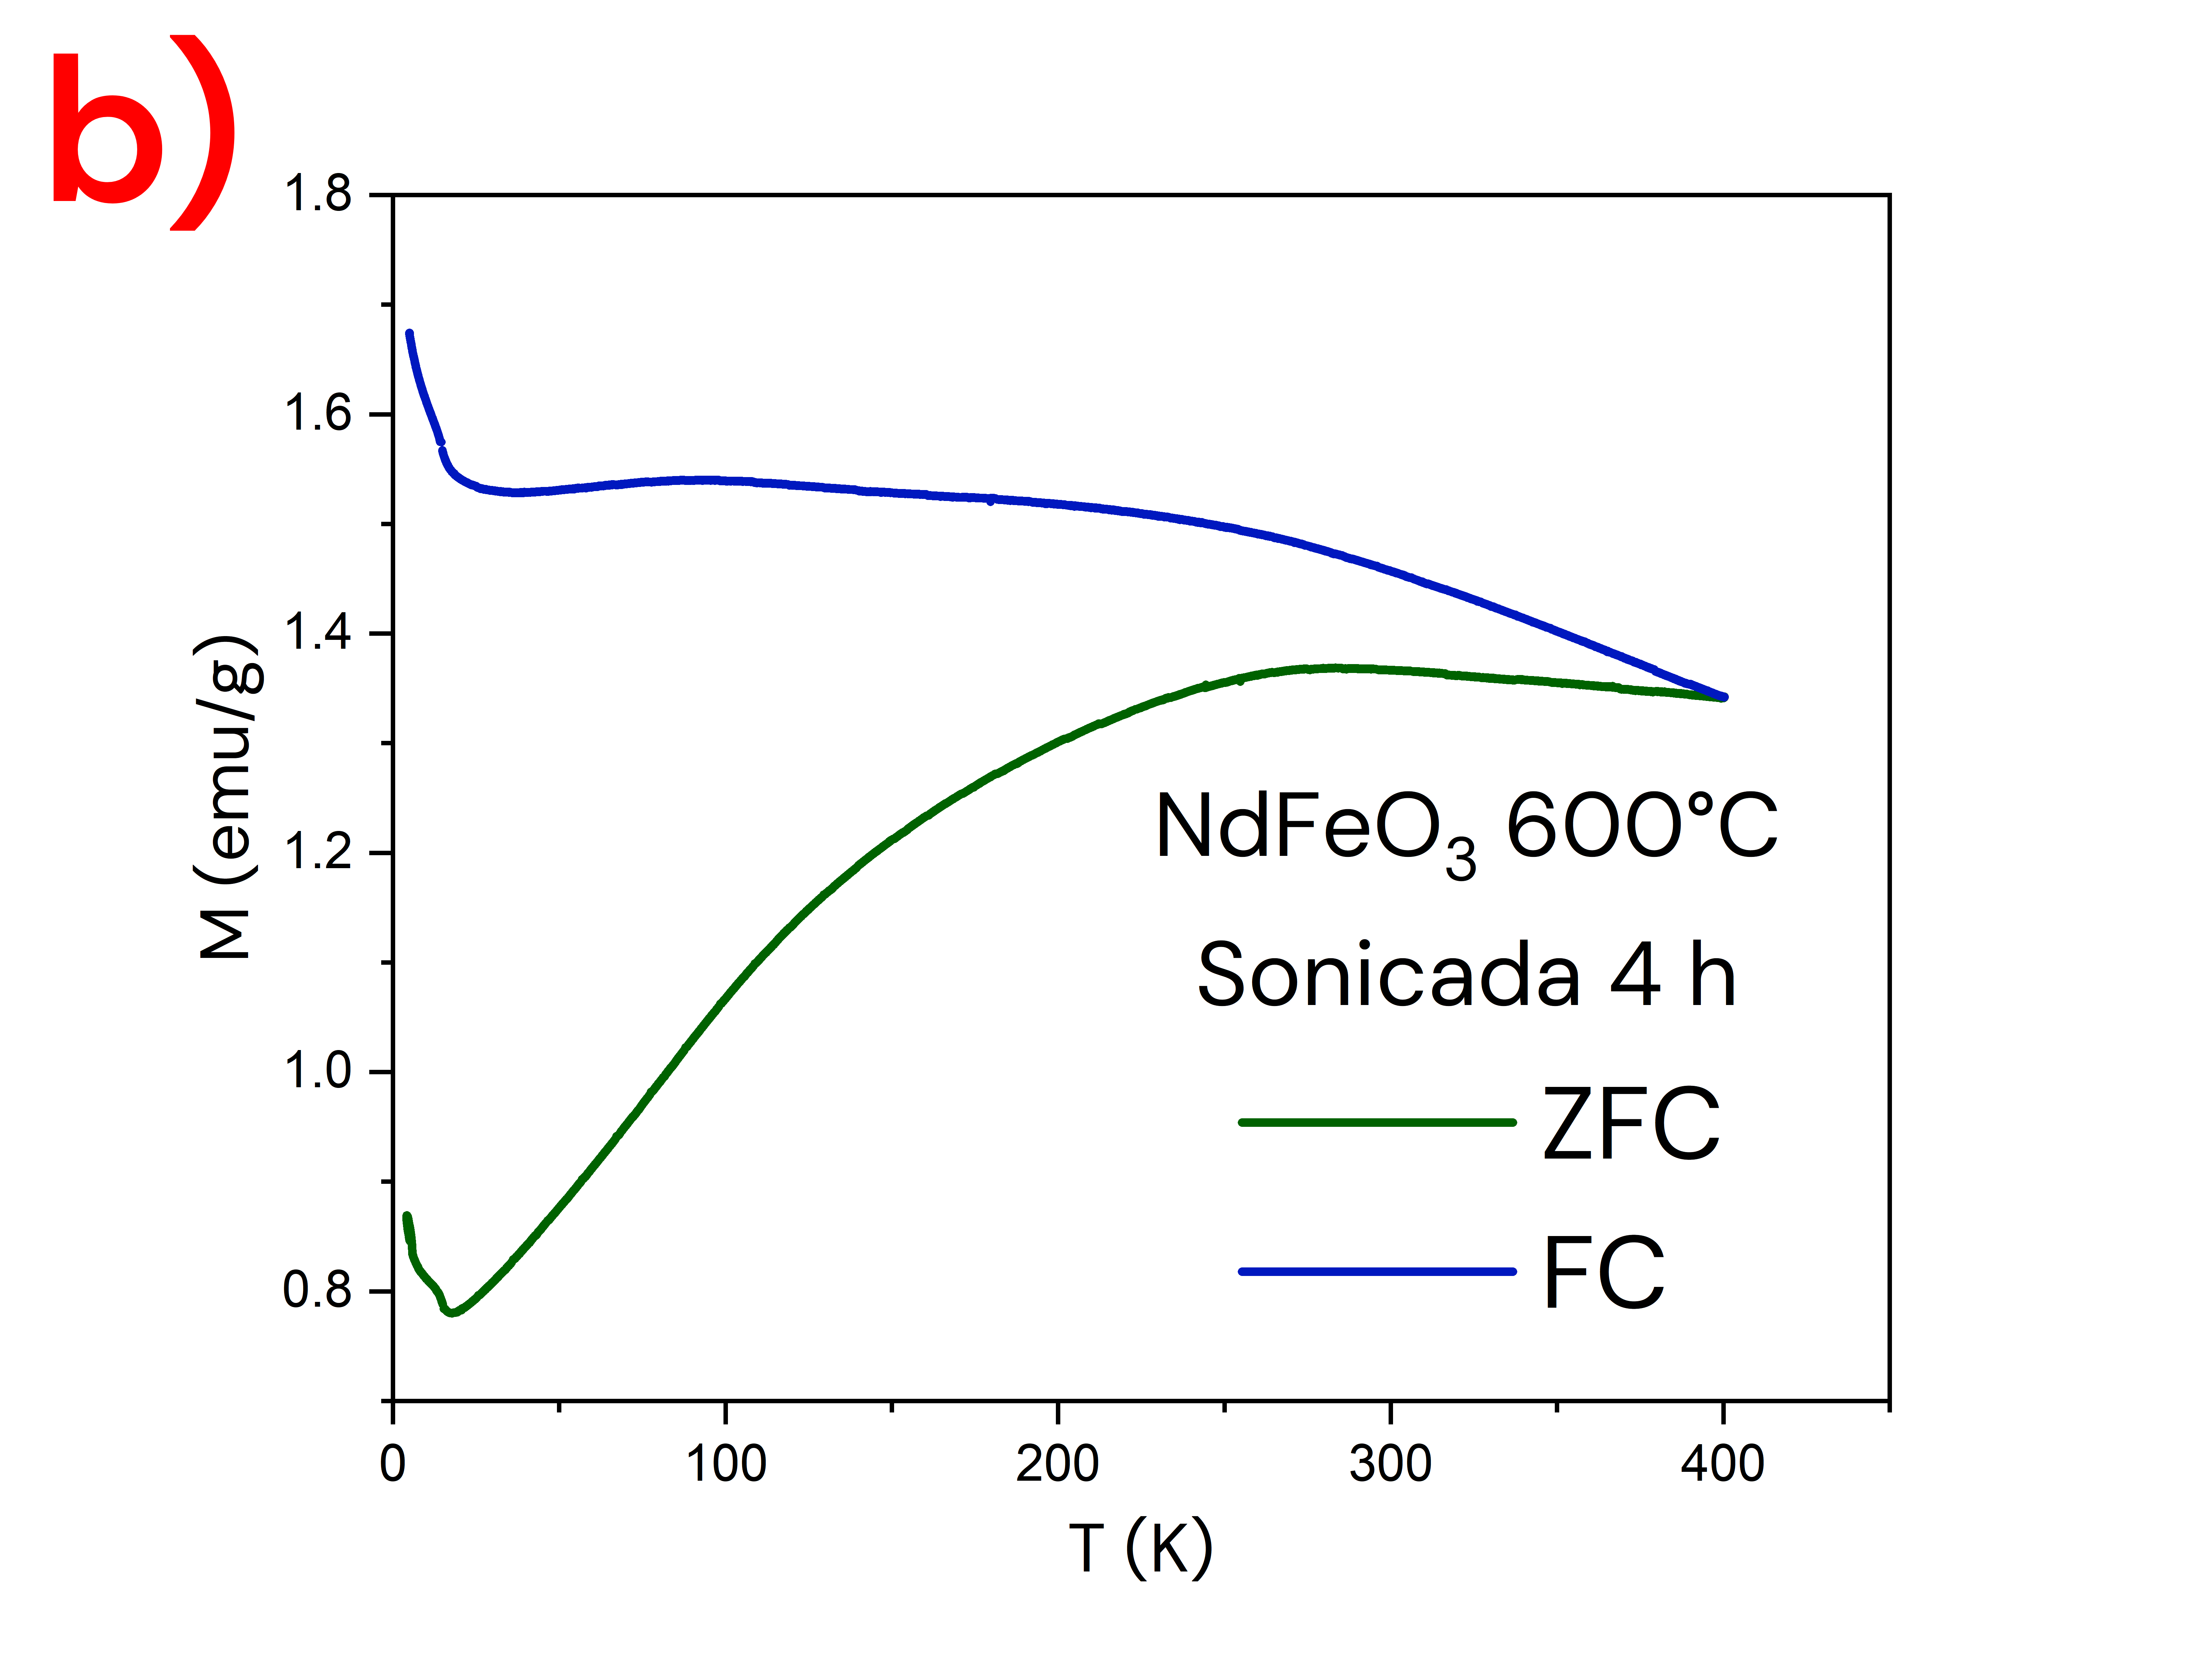
\includegraphics[width=0.45\textwidth]{fig/MvTNd-S.png}
    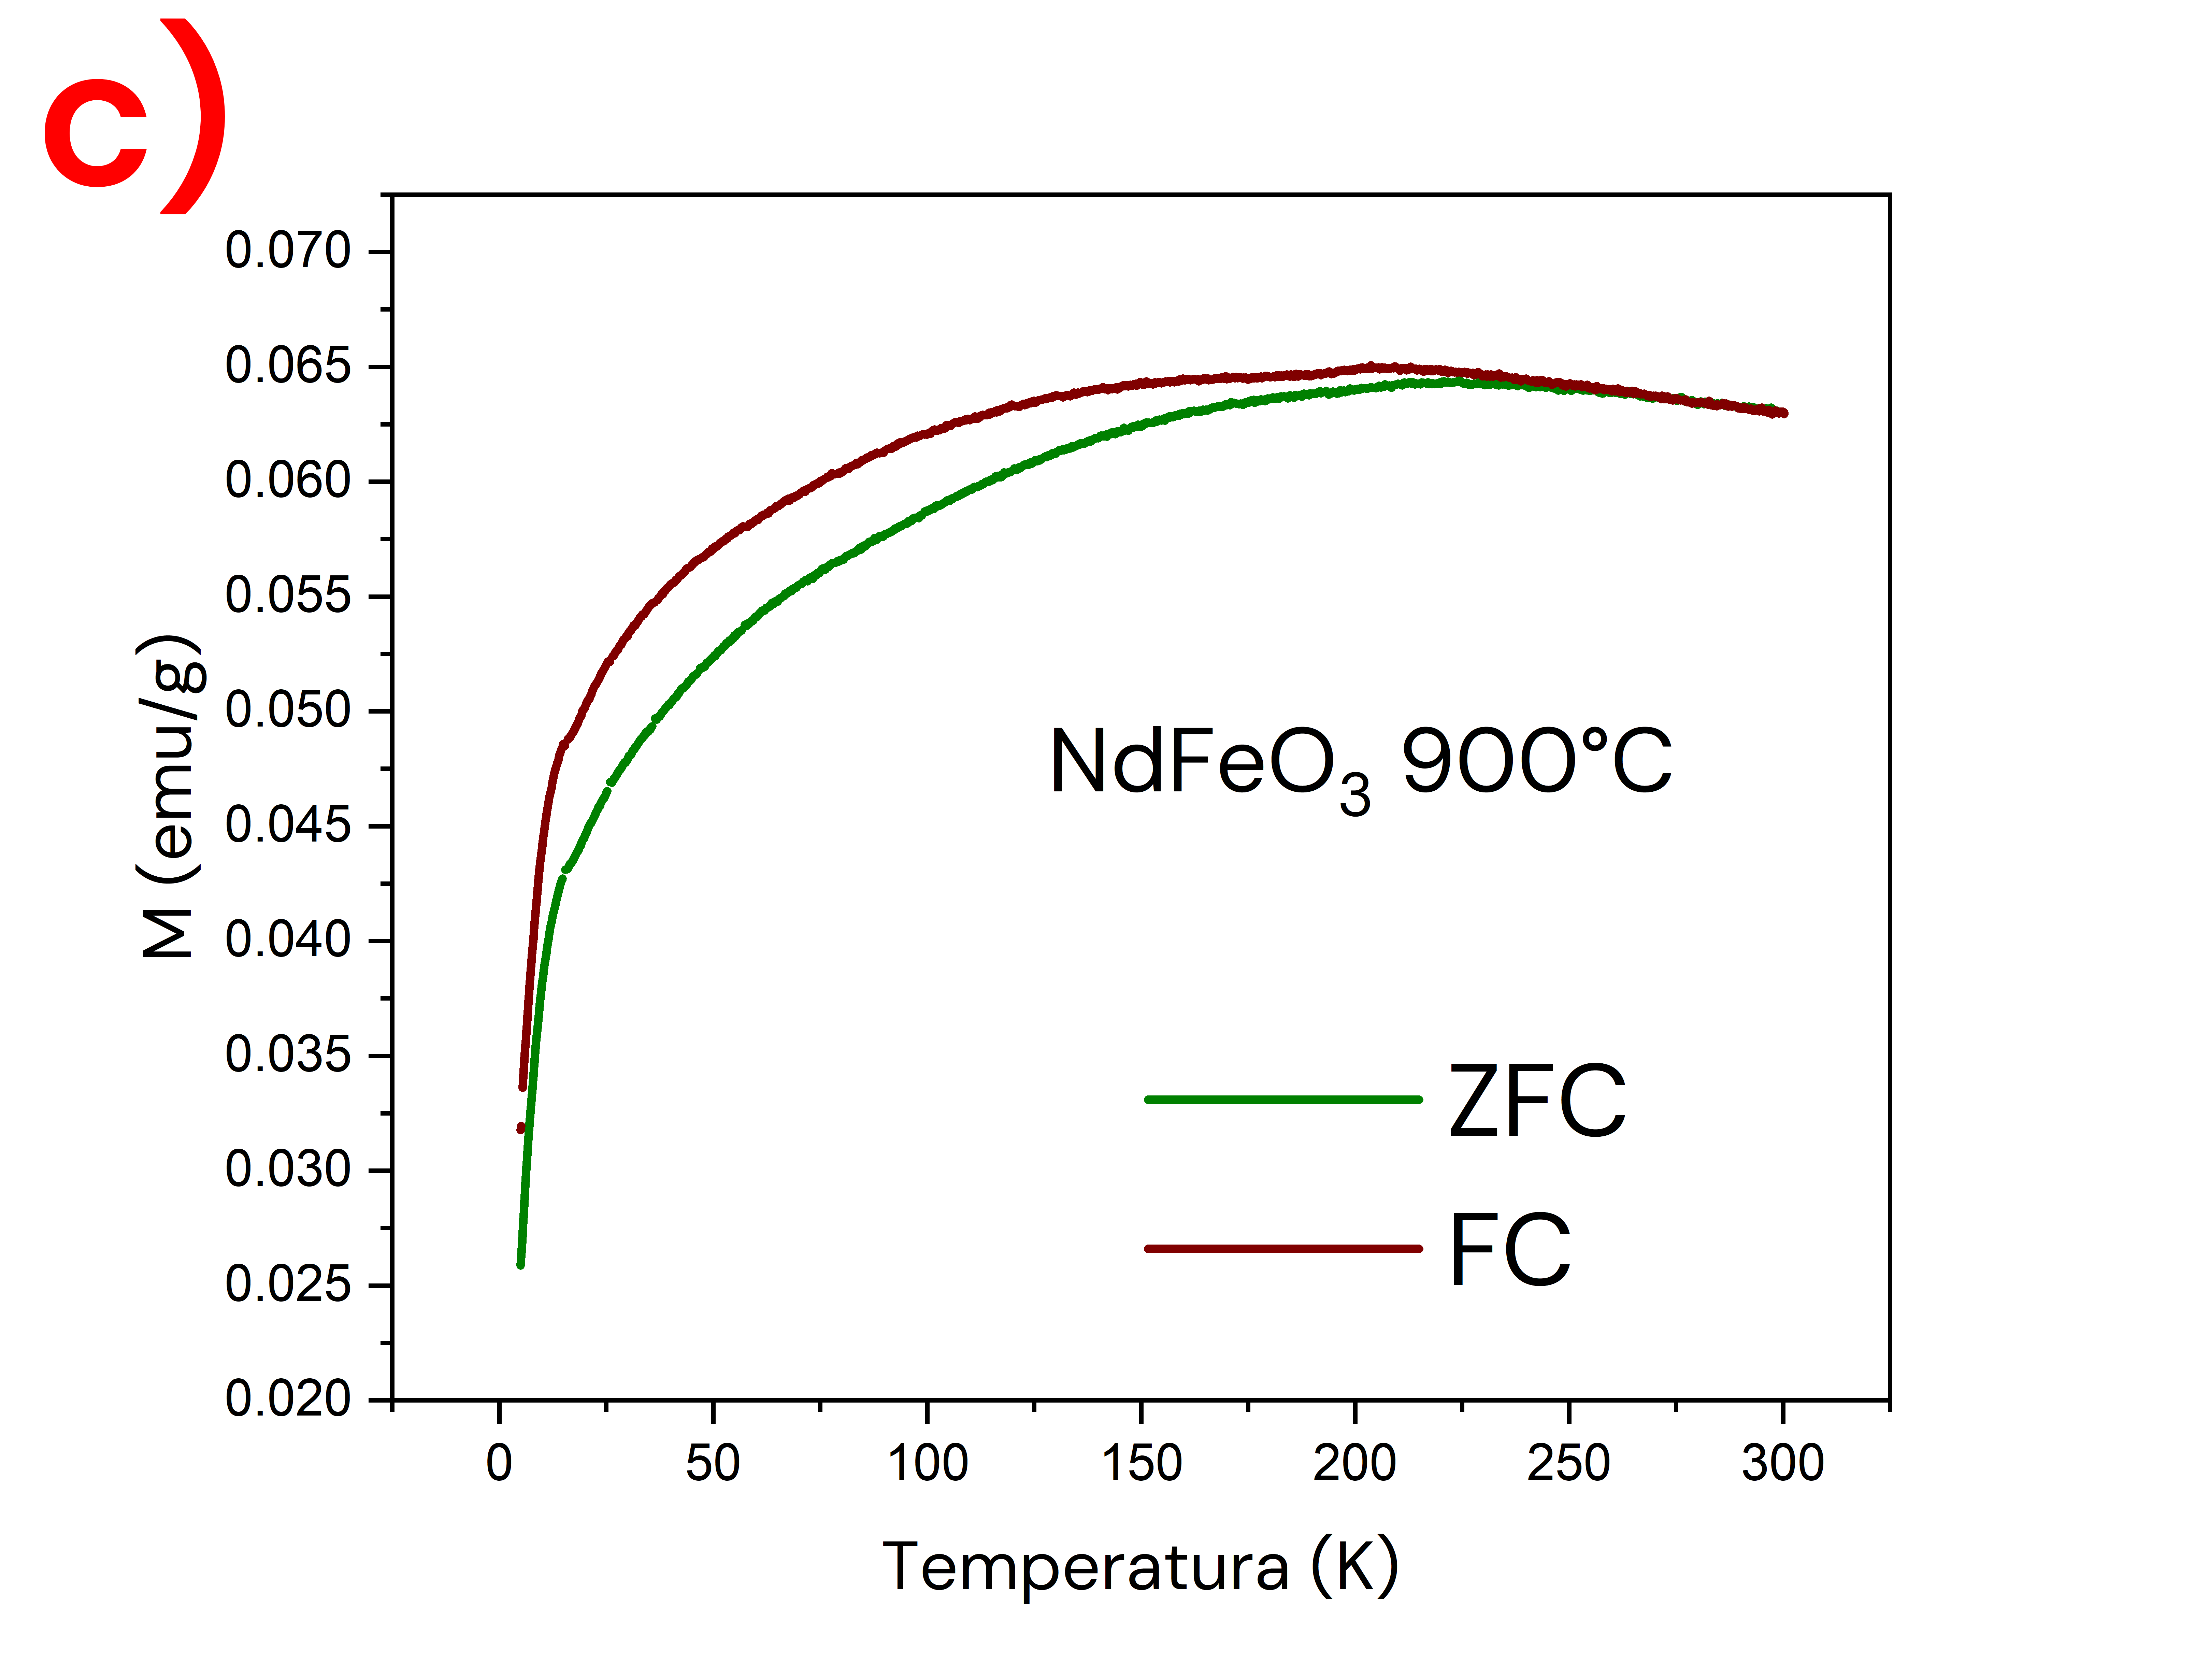
\includegraphics[width=0.45\textwidth]{fig/MvTNd900.png}
    \caption{Curvas $M$ contra $T$ para las muestras de \neod{}: a) sin sonicar y b) sonicada.}
    \label{fig:MvTNd}
\end{figure}
\begin{figure}[H]
    \centering
    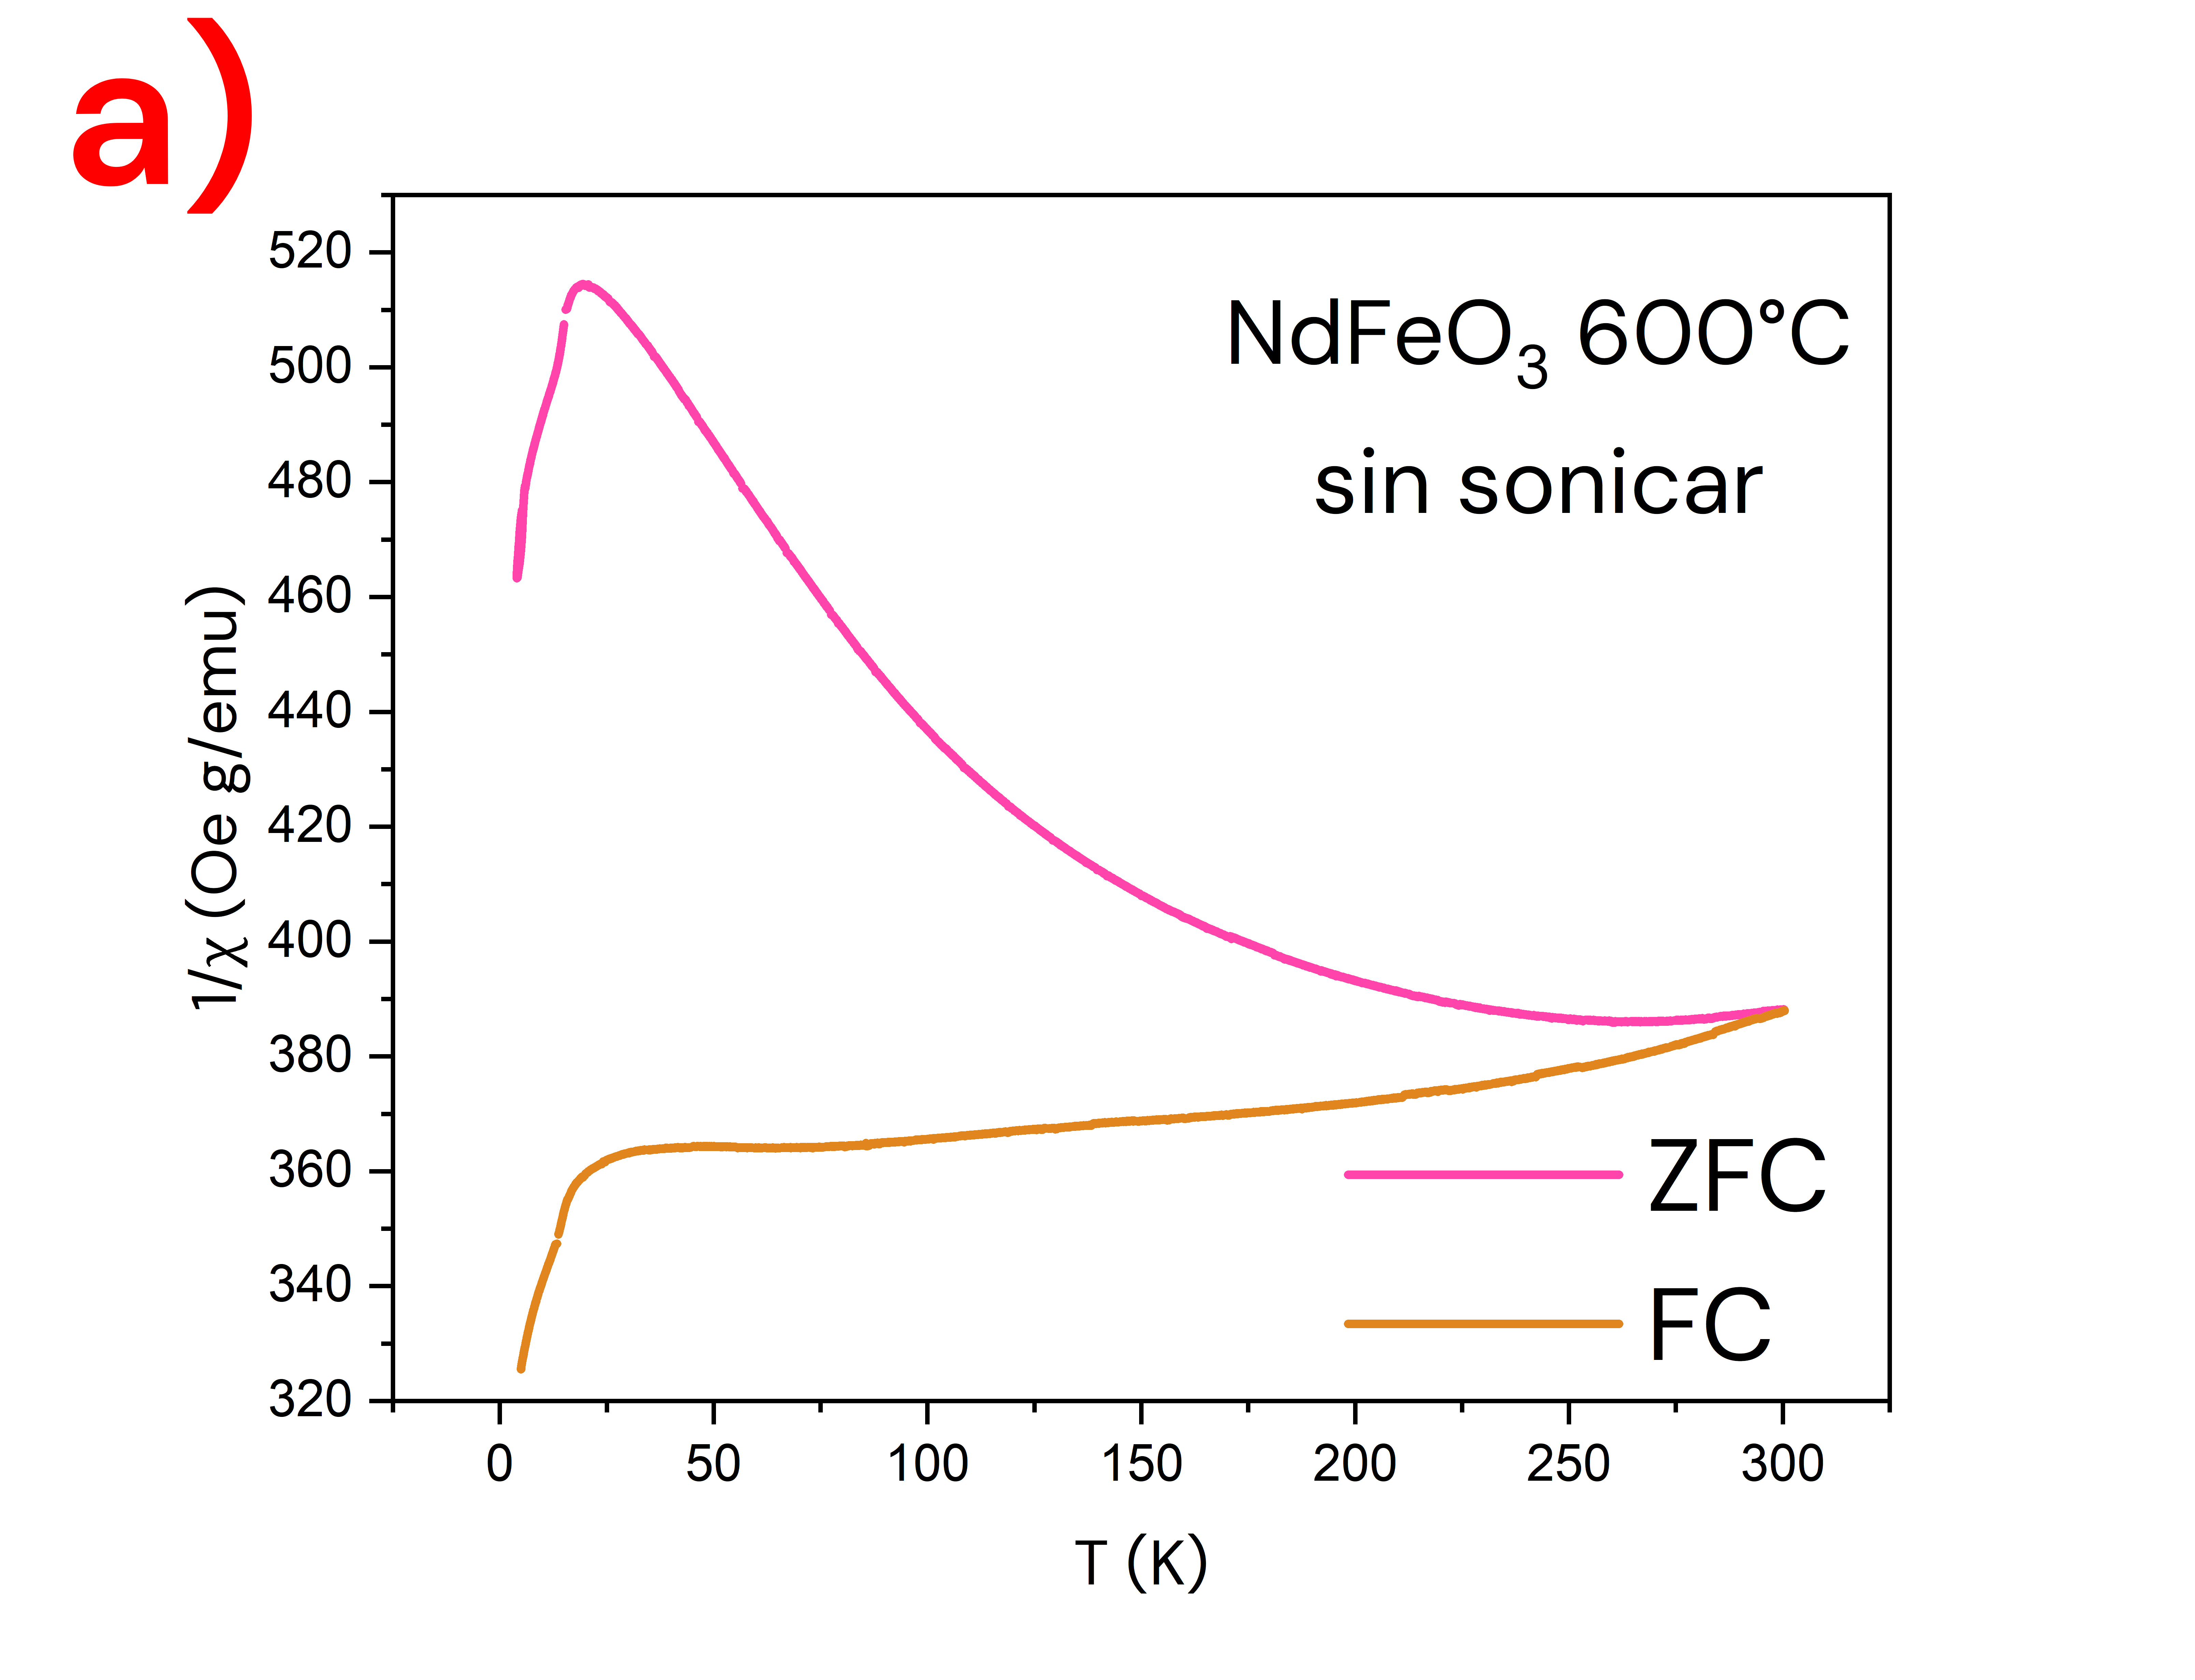
\includegraphics[width=0.45\textwidth]{fig/chivTNd.png}
    \quad
    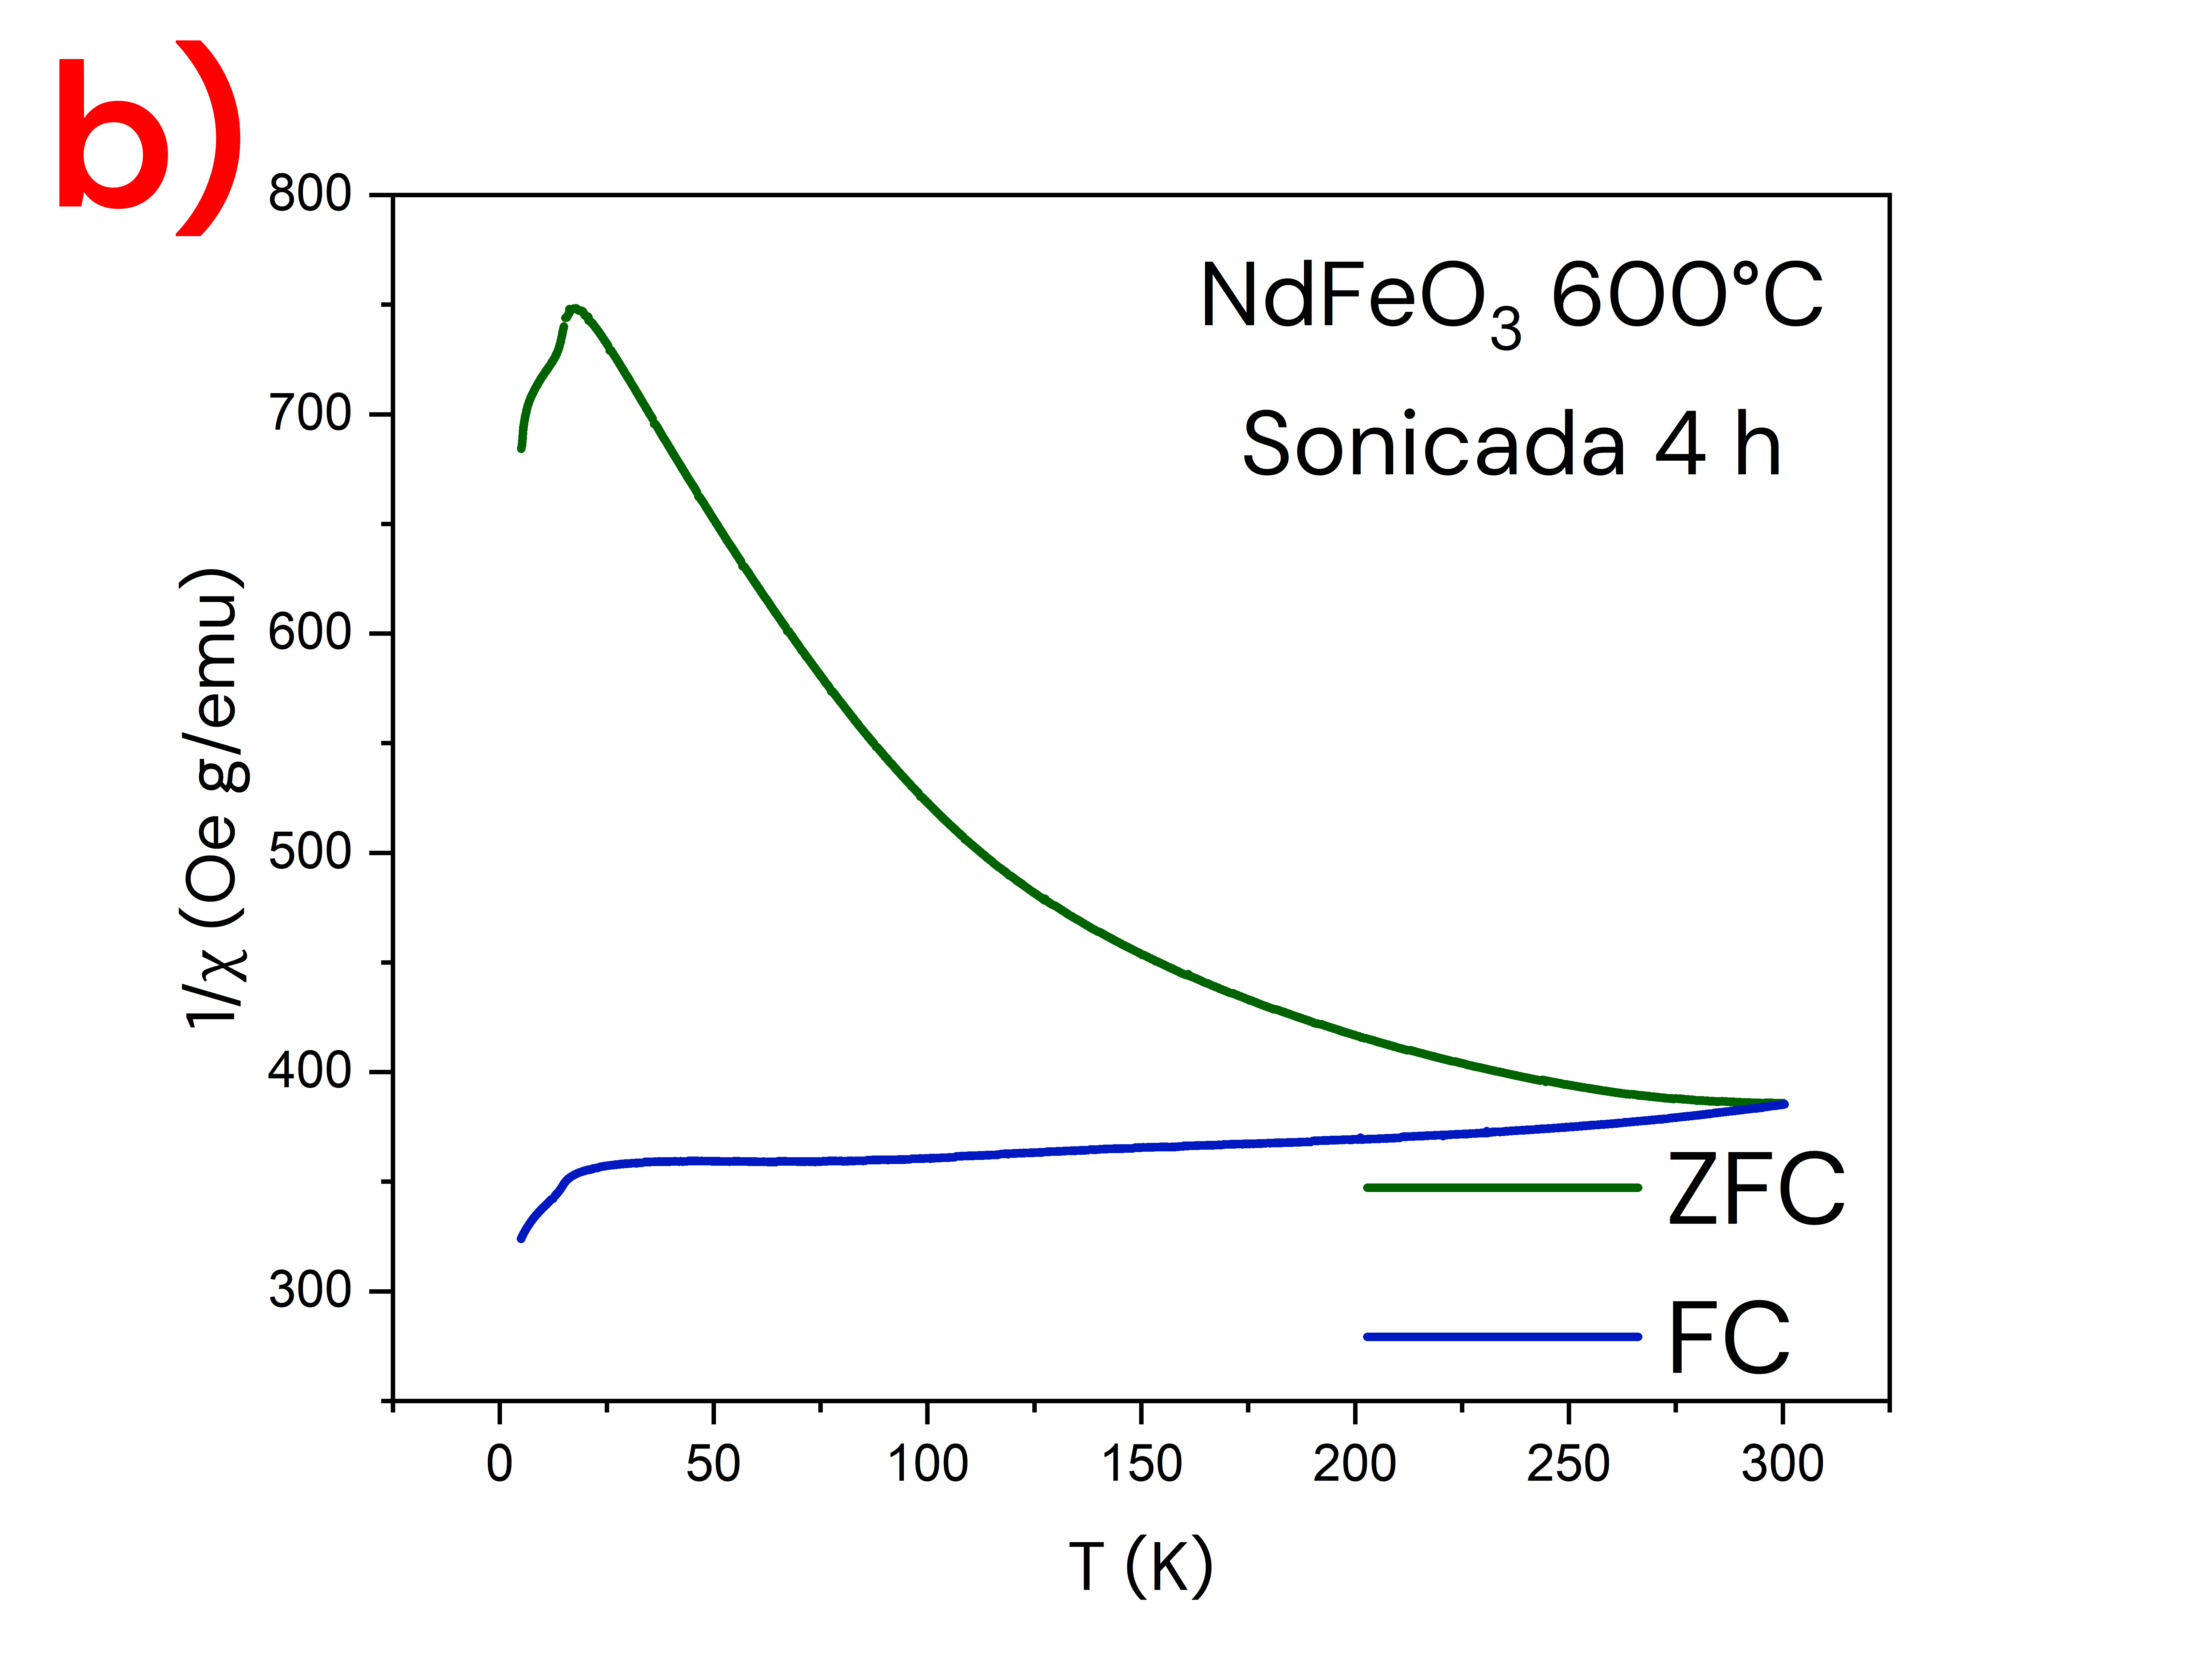
\includegraphics[width=0.45\textwidth]{fig/chivTNd-S.png}
    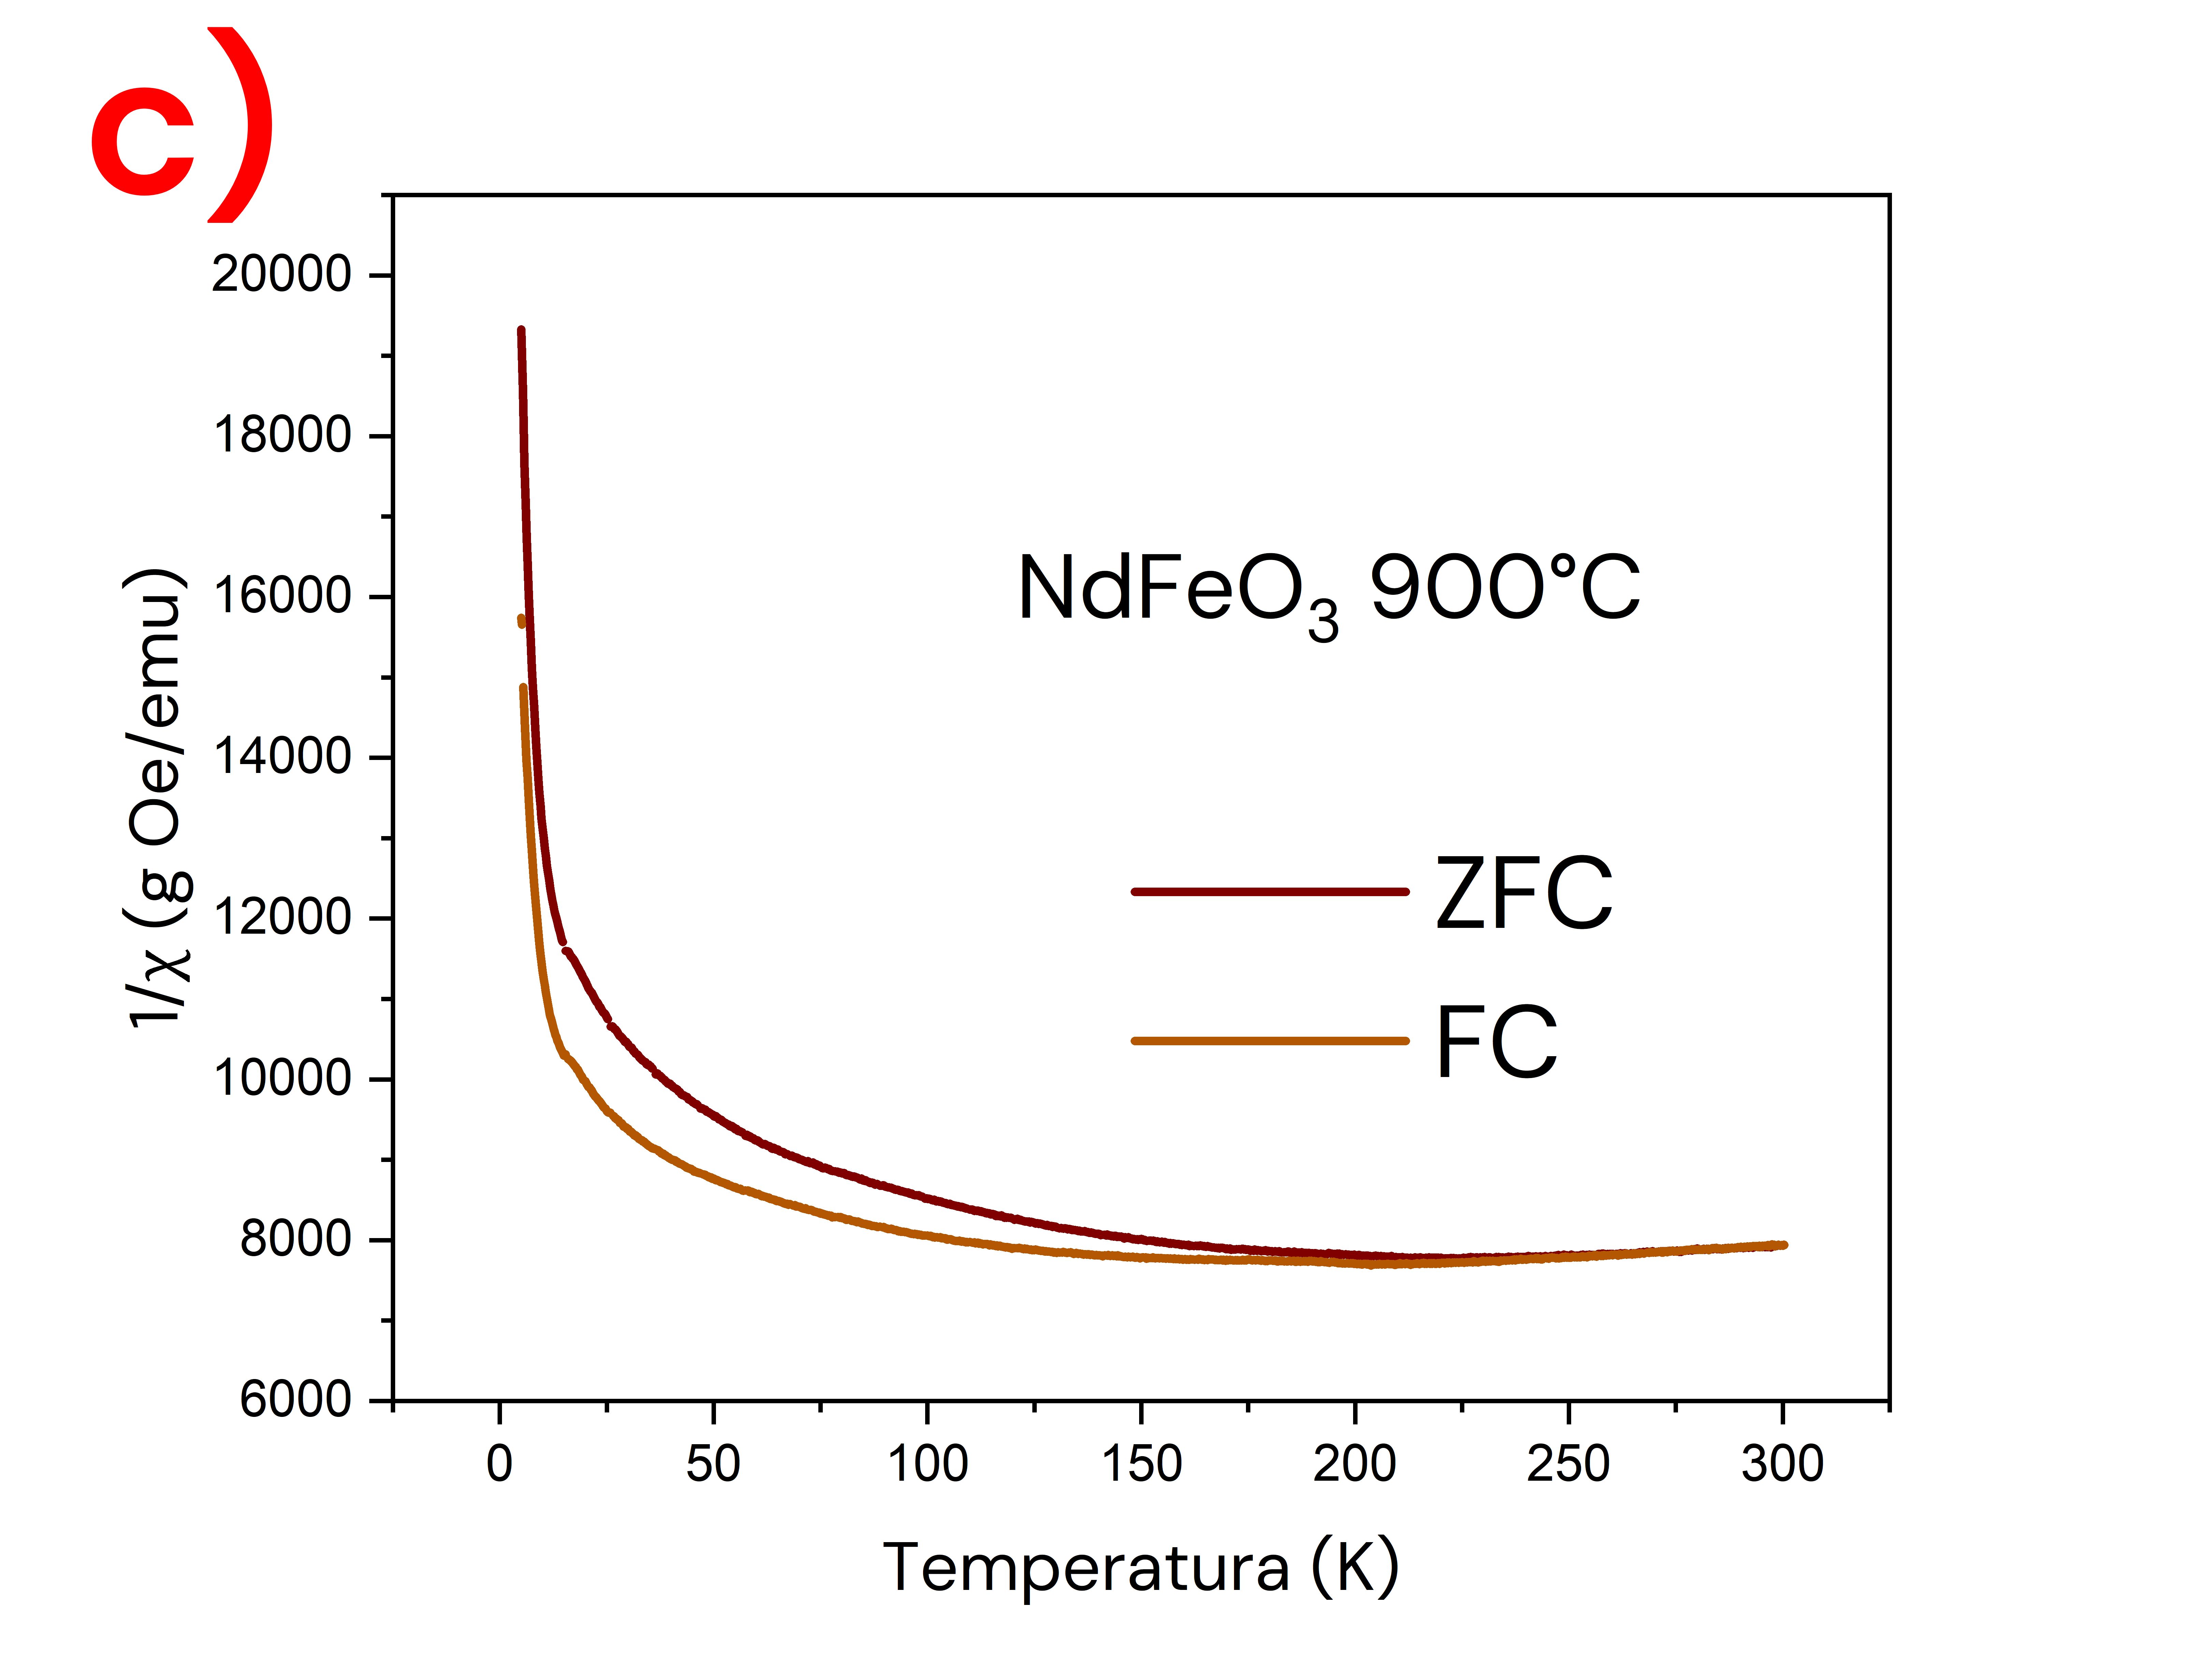
\includegraphics[width=0.45\textwidth]{fig/chivTNd900.png}
    \caption{Curvas $\chi$ contra $T$ para las muestras de \neod{}: a) sin sonicar y b) sonicada.}
    \label{fig:chivTNd}
\end{figure}
No se observa un cambio significativo entre las muestras sonicada y sin sonicar, pero sí un cambio con la temperatura de calcinación.

Para las muestras calcinadas a 600\gradoC{} se observa un reordenamiento magnético alrededor de los 20 K (24.10$\pm$0.064 K para la muestra sin sonicar, 20.82$\pm$0.036 K para la muestra sonicada), donde ocurre un mínimo local de $M$ y $\chi$, además de una separación considerable de las curvas ZFC y FC, la cual se reduce a medida que aumenta la temperatura. Por otra parte, para la muestra calcinada a 900\gradoC{} no se observa esta transición de fase, y las curvas ZFC y FC son muy similares entre sí.
\subsubsection{Curvas de polarización}
En las figuras \ref{fig:nd100v} y \ref{fig:nd2000v} se reportan las curvas $P$ vs $E$ de las muestras de \neod{} sinterizadas.
\begin{figure}[H]
    \centering
    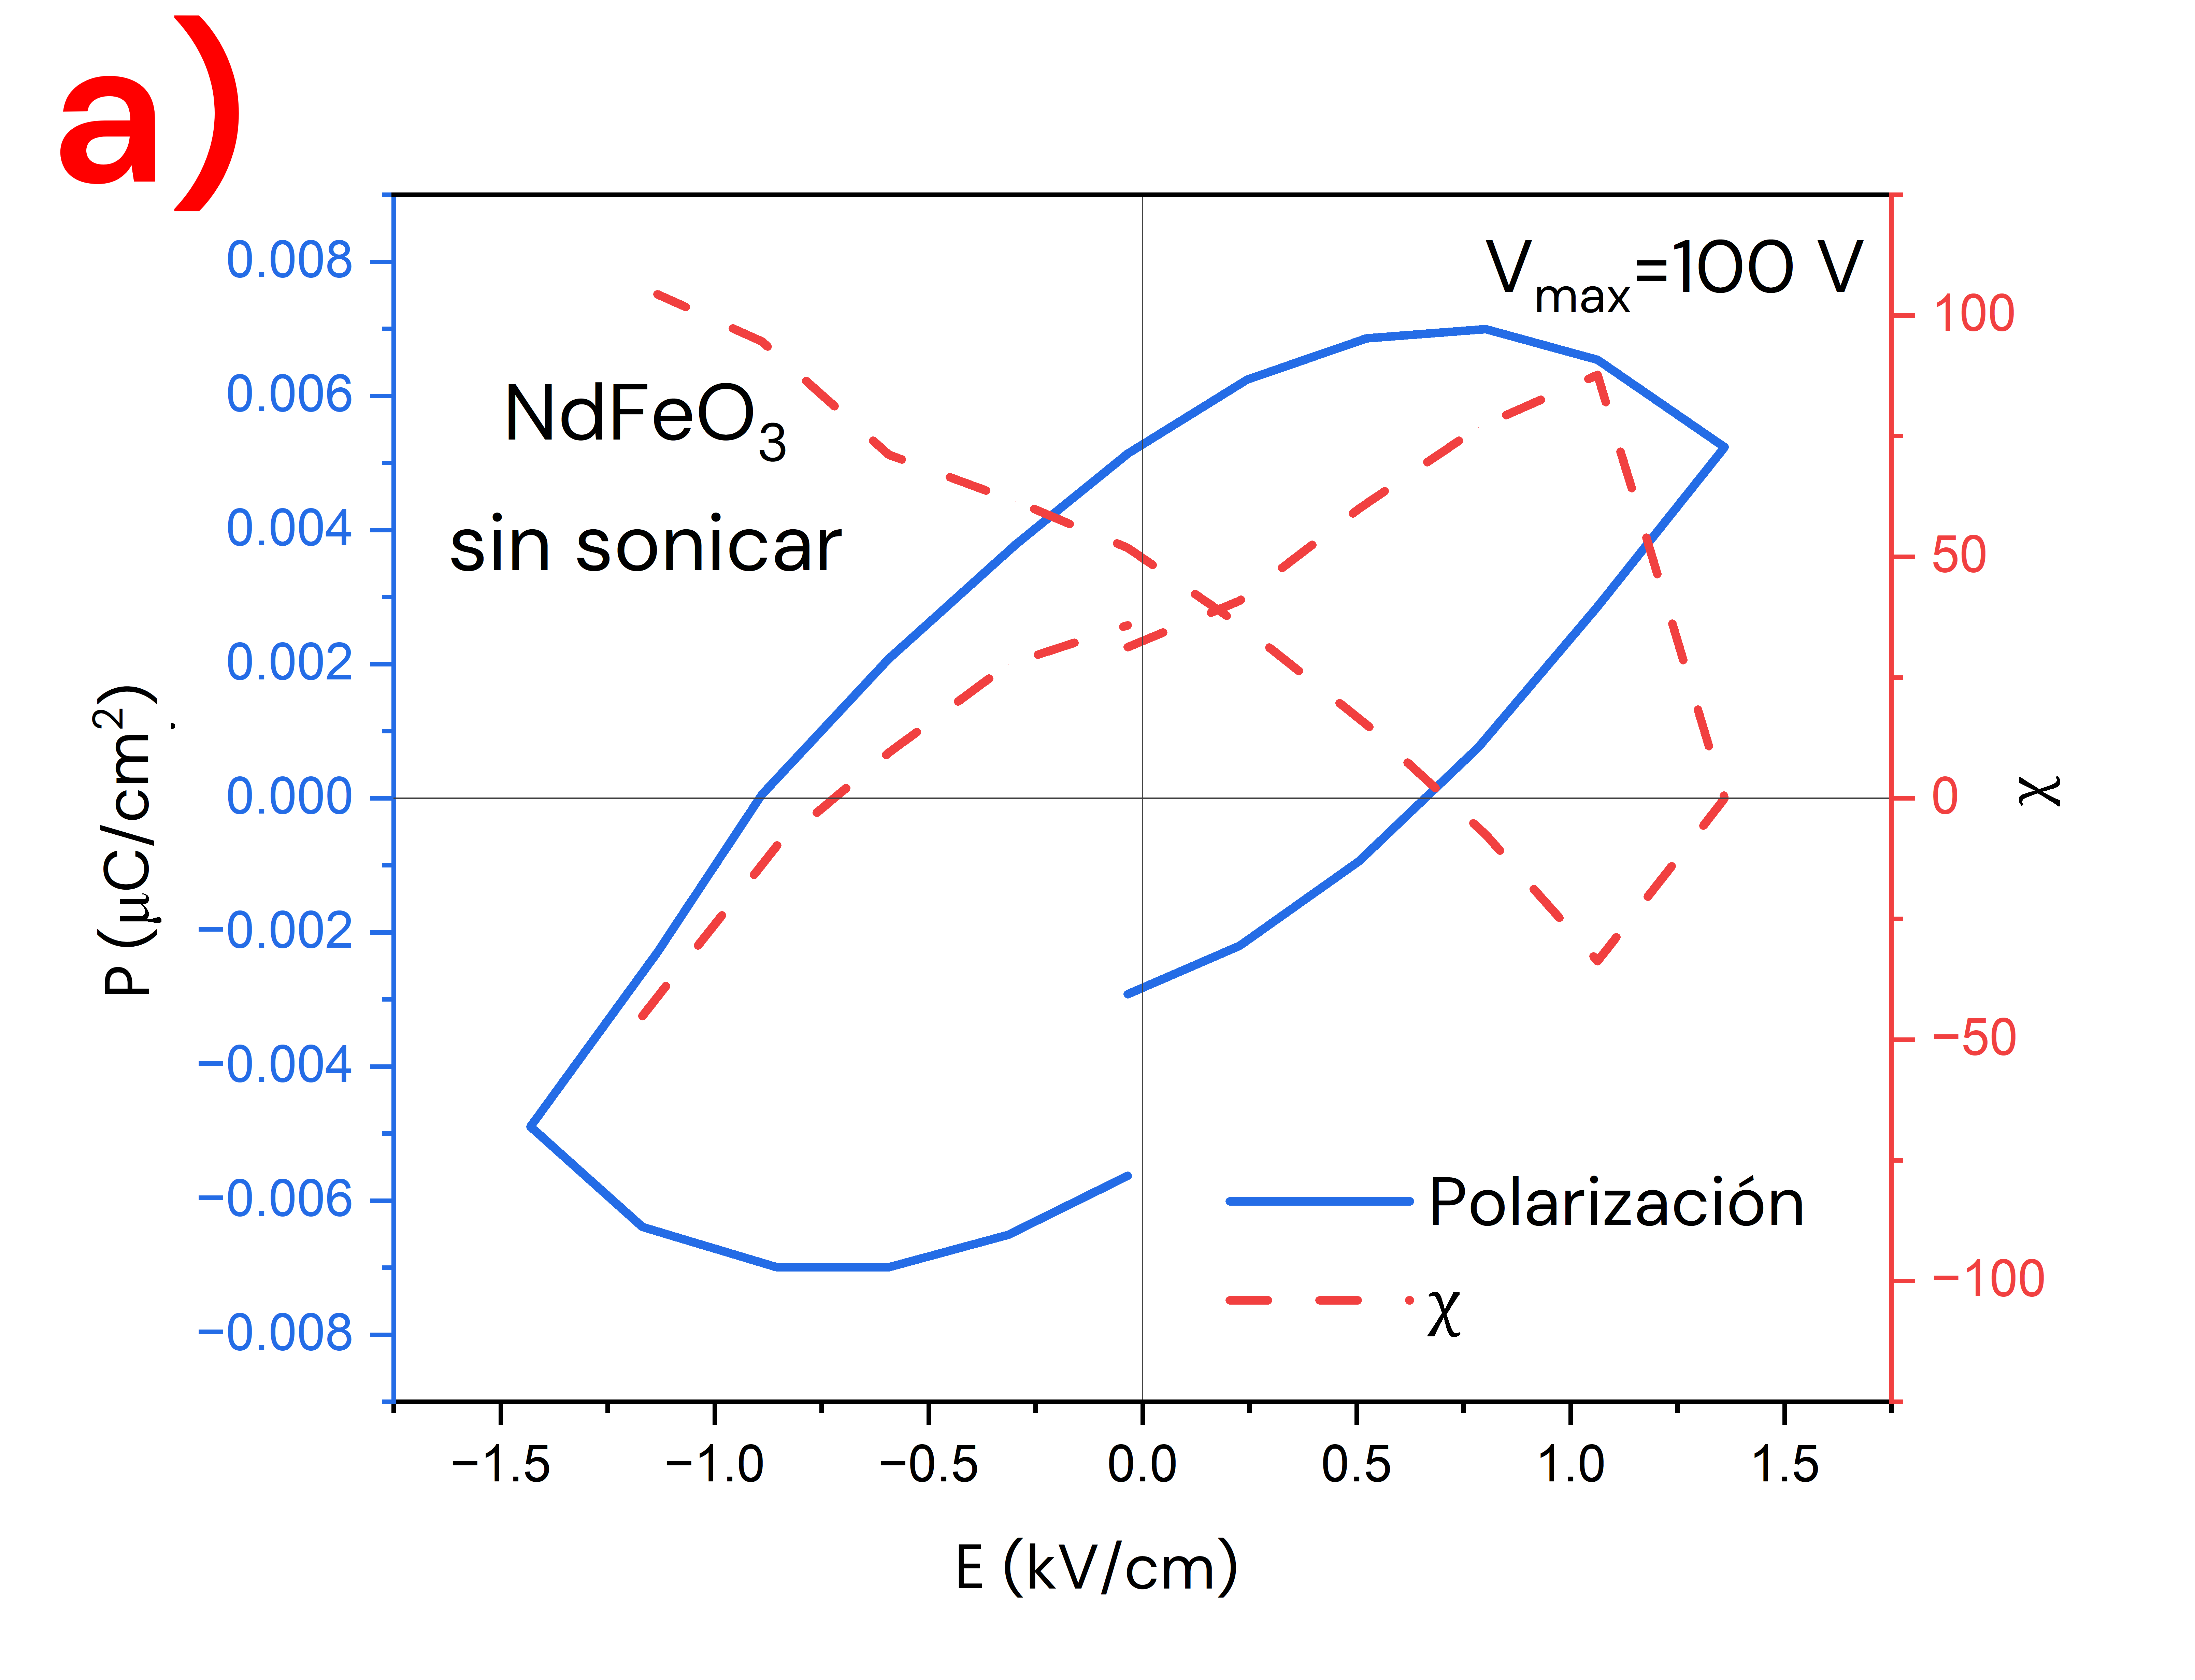
\includegraphics[width=0.45\textwidth]{fig/PENdFeO3100V.png}
    \quad
    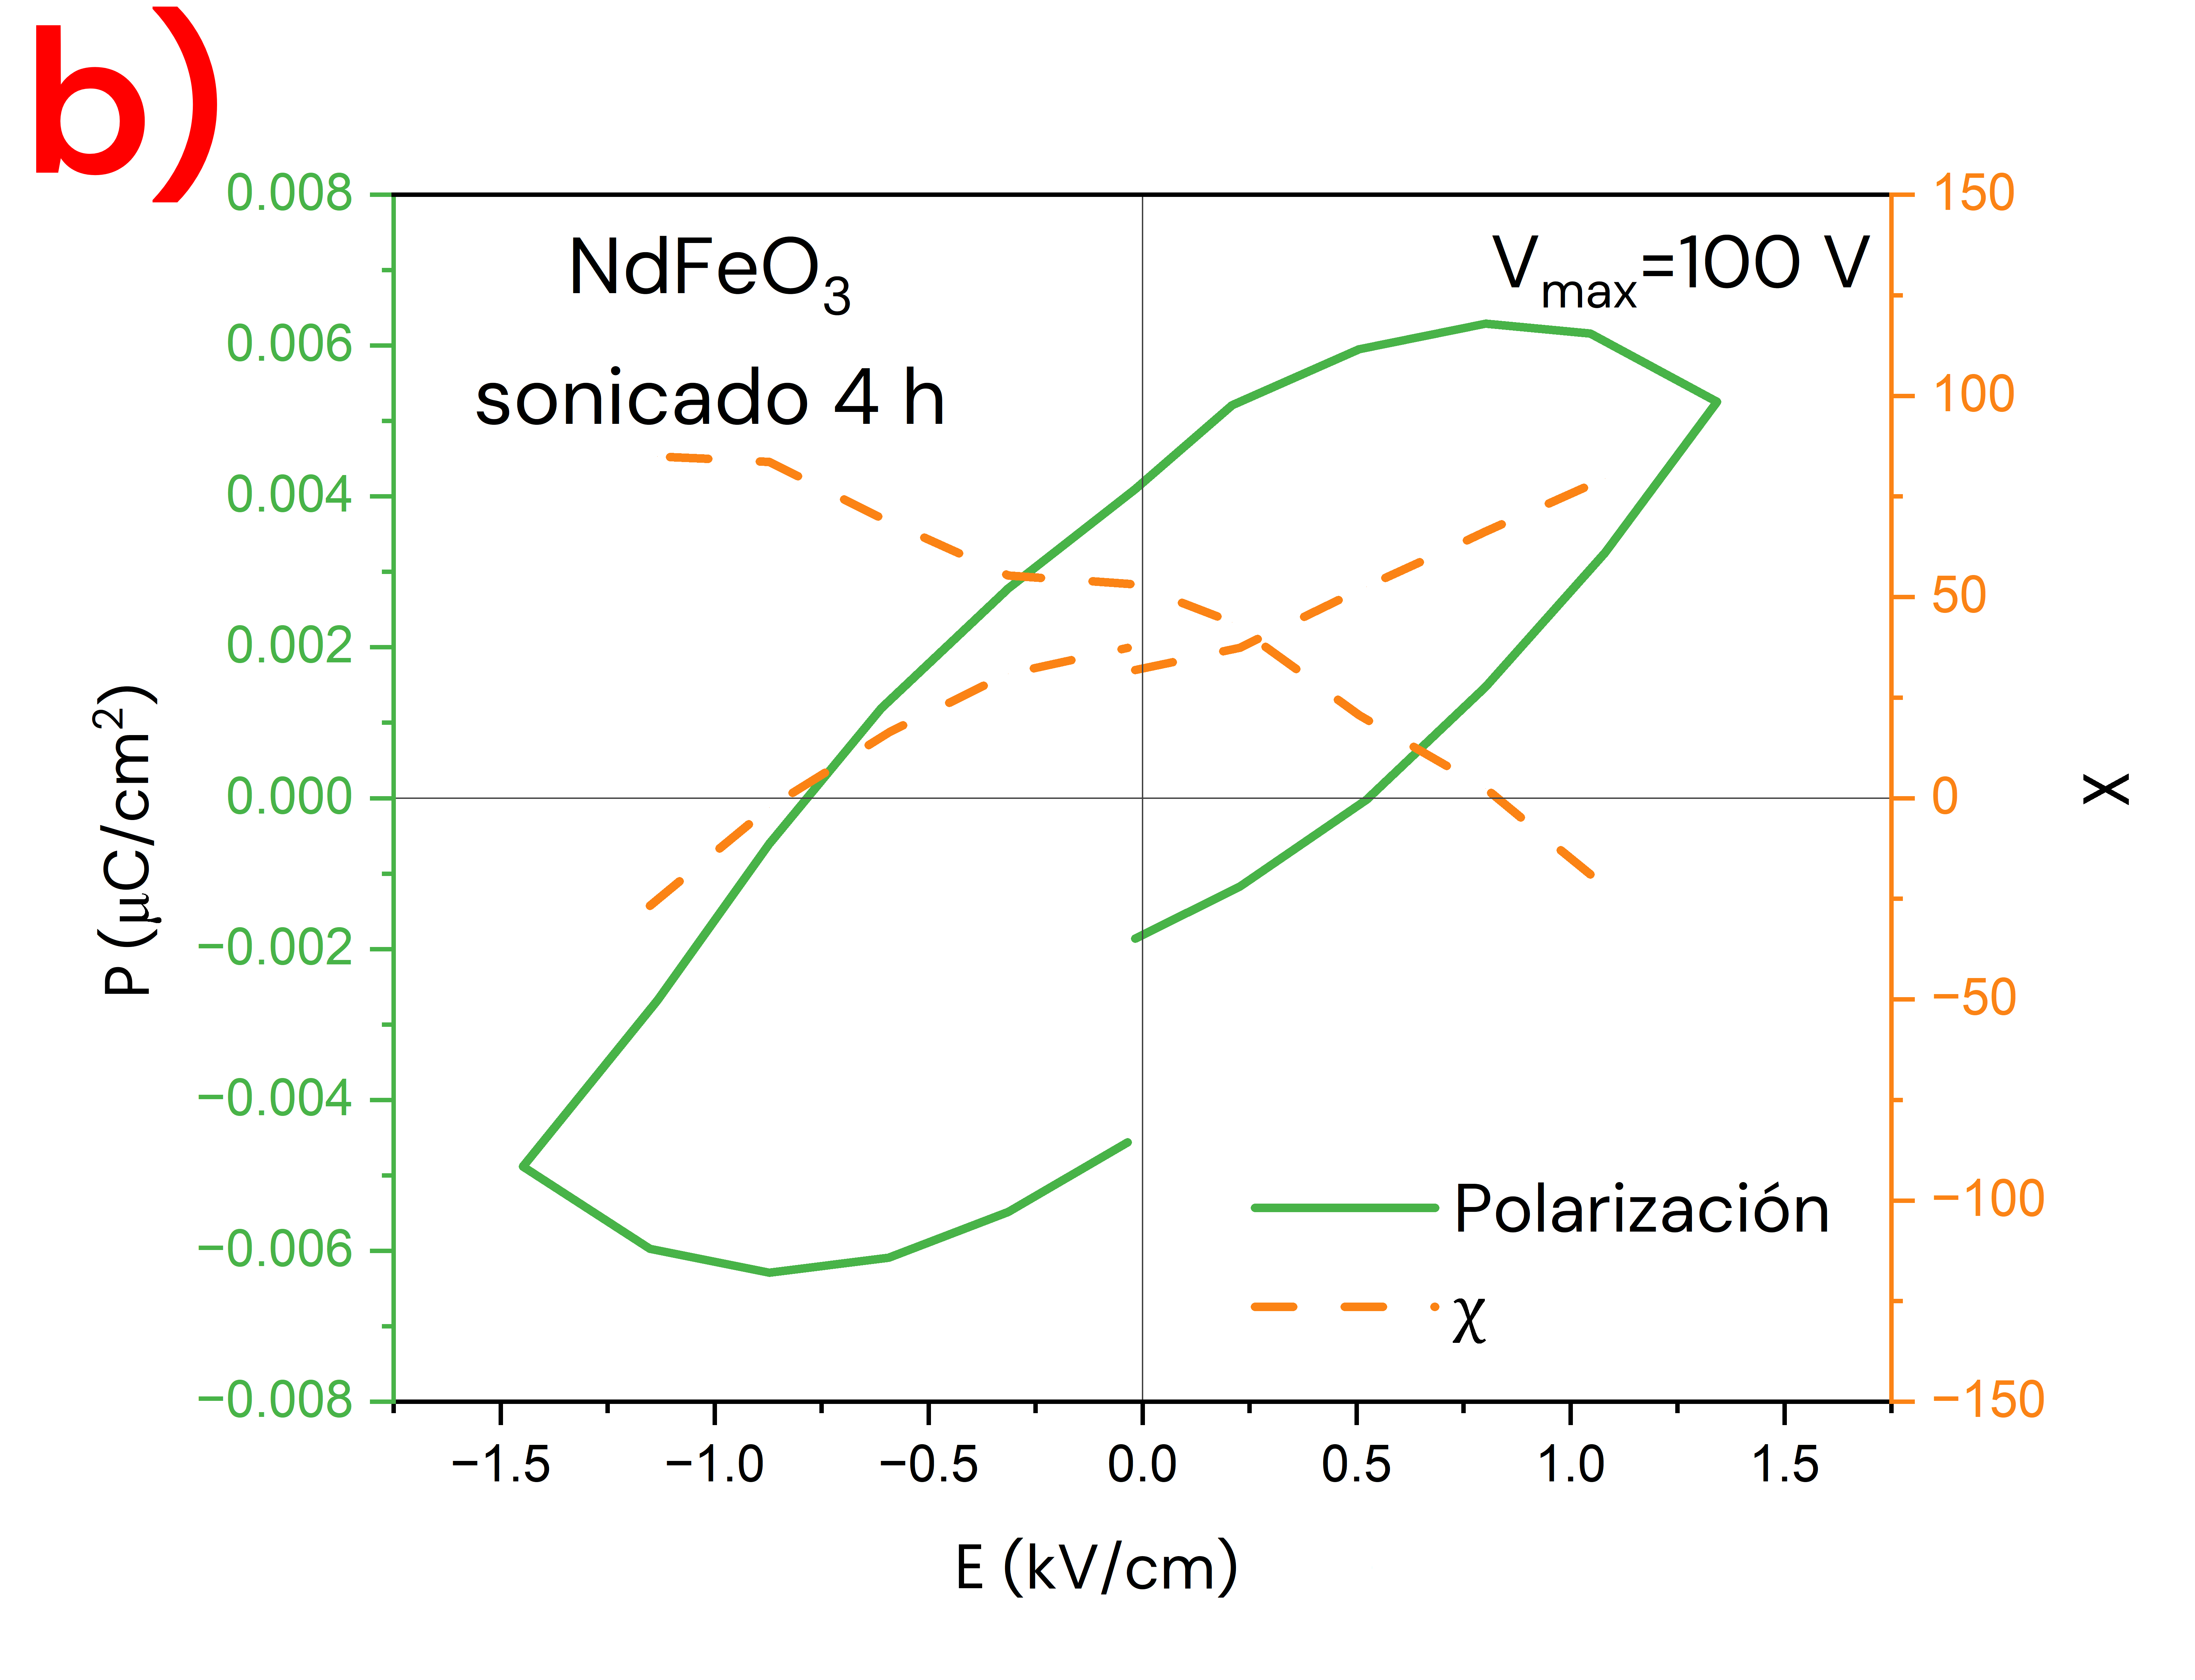
\includegraphics[width=0.45\textwidth]{fig/PENdFeO3-S100V.png}
    \caption{Curvas $P$ contra $E$ (eje izquierdo) y $\chi$ contra $E$ (eje derecho) con $V_\text{max}=100$ V de las muestras de \neod{}: a) sin sonicar y b) sonicada 4 h.}
    \label{fig:nd100v}
\end{figure}
\begin{figure}[H]
    \centering
    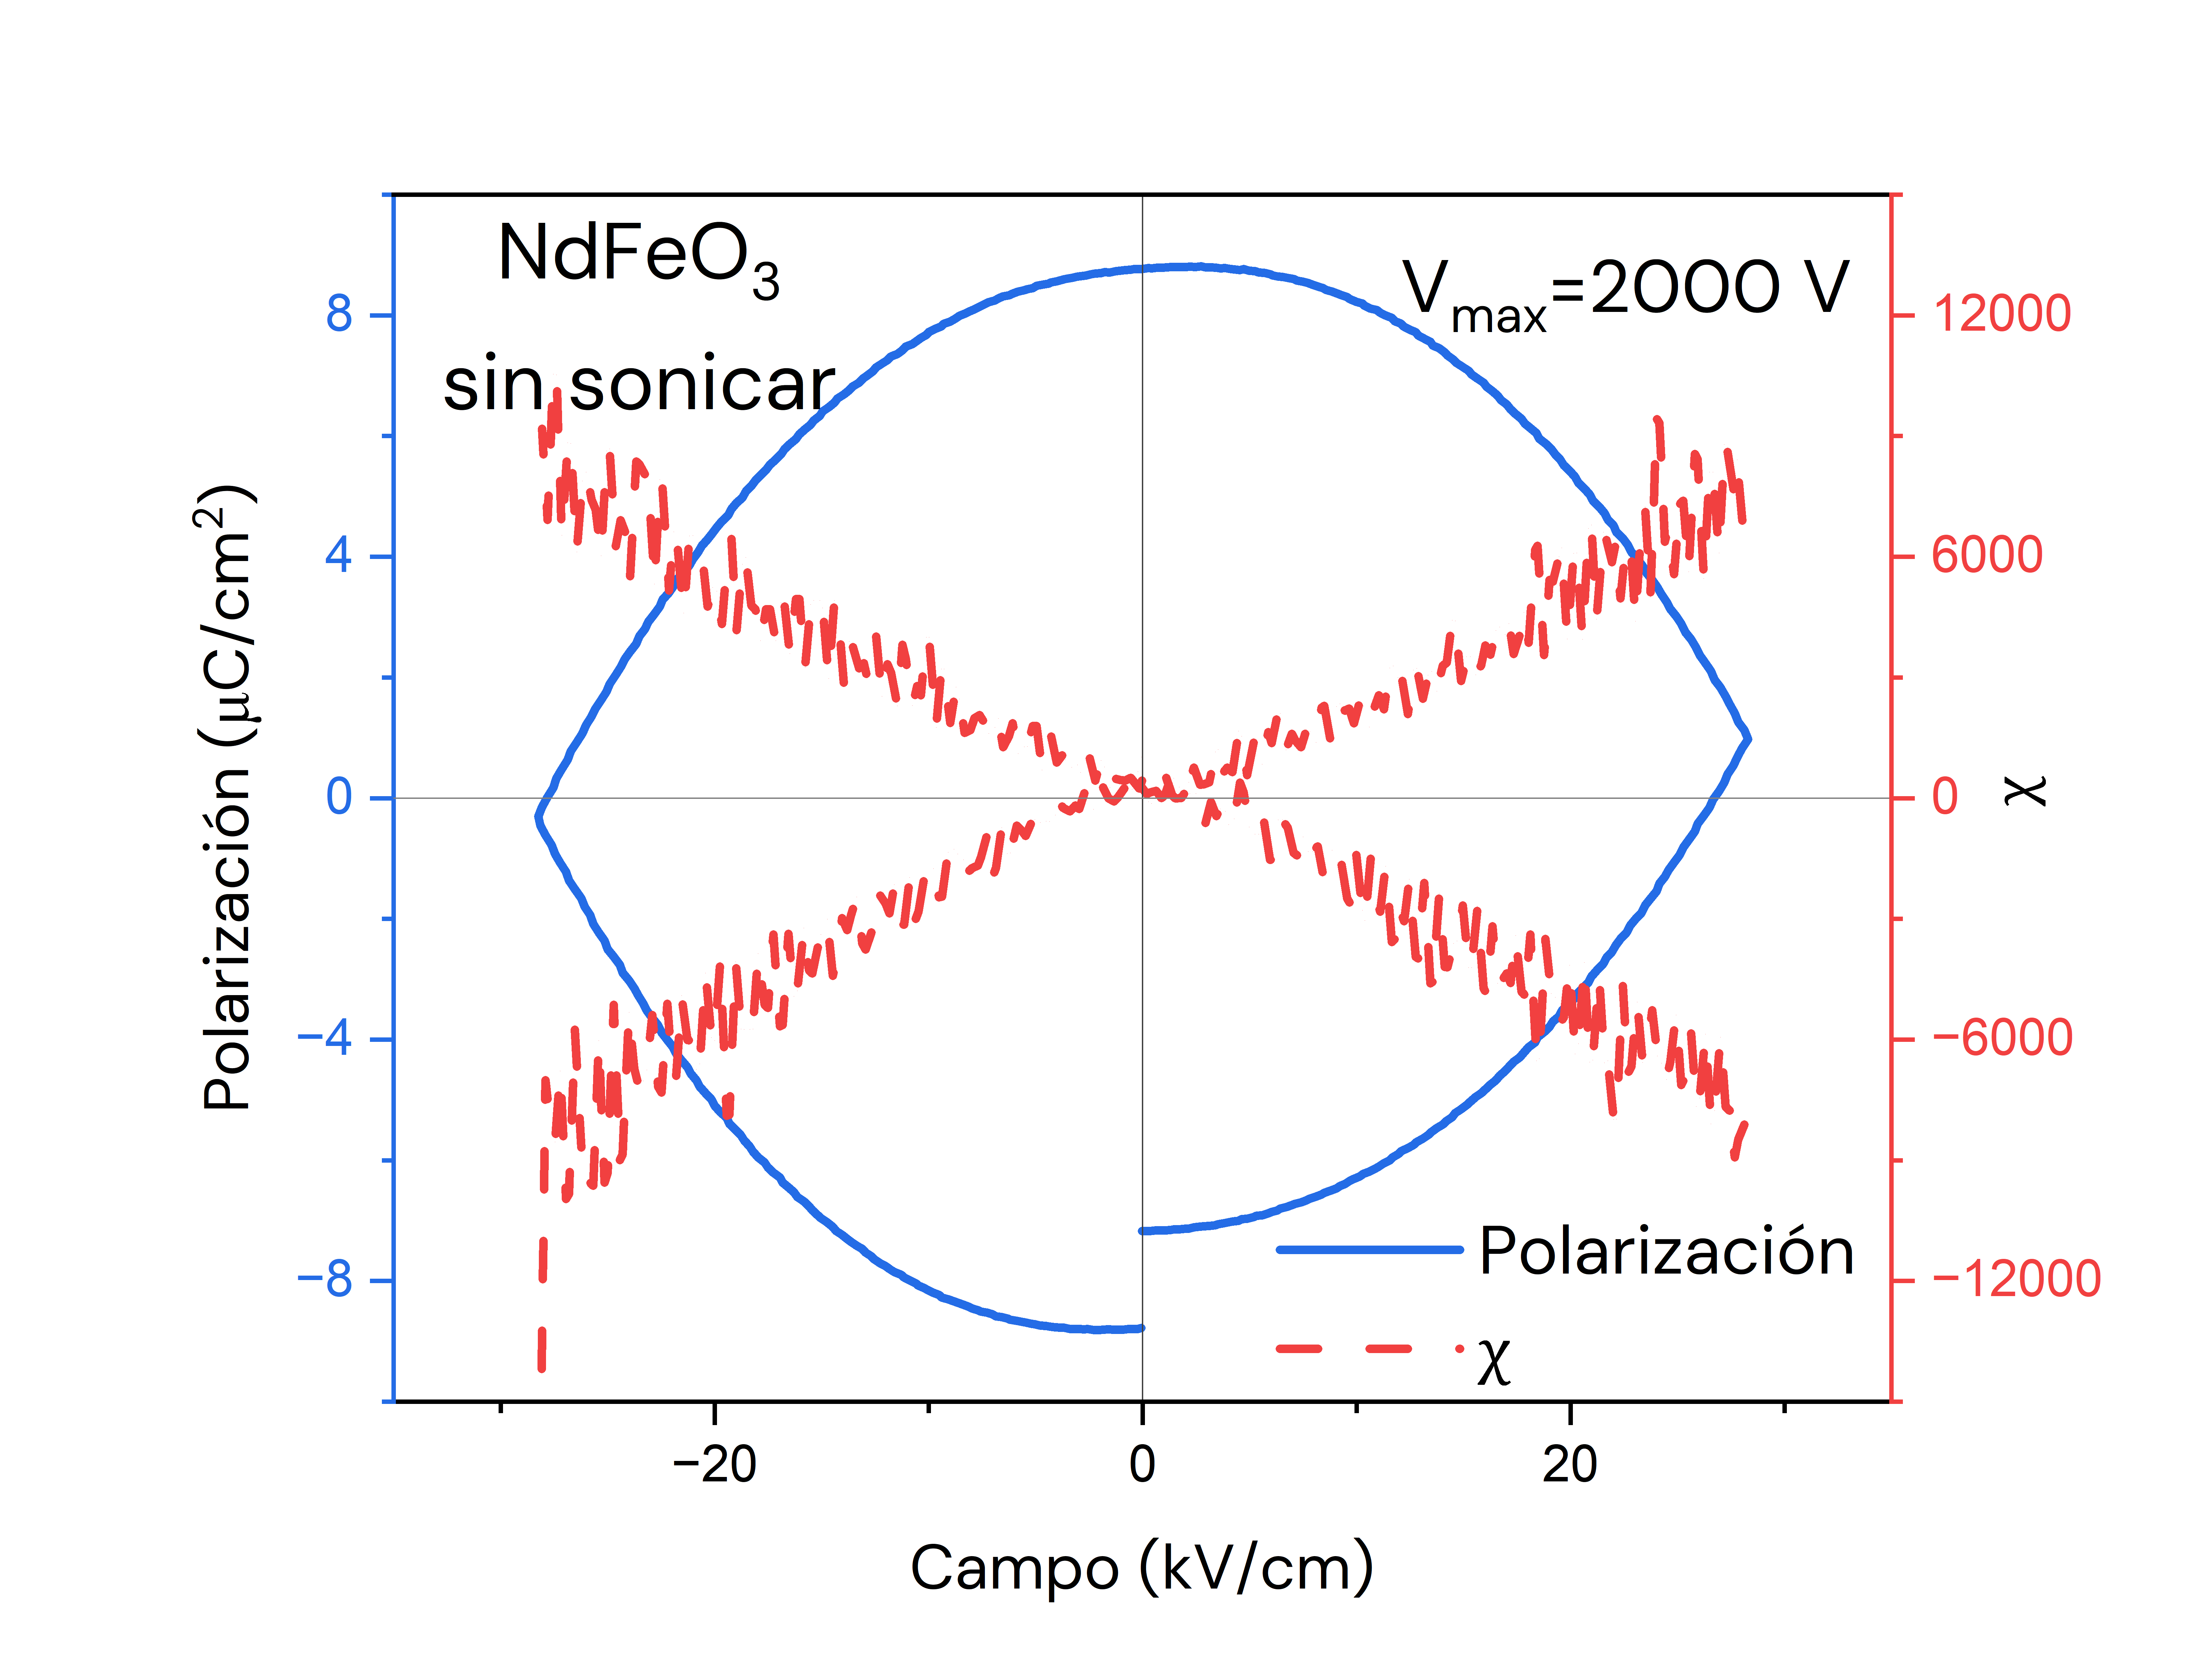
\includegraphics[width=0.45\textwidth]{fig/PENdFeO32000V.png}
    \quad
    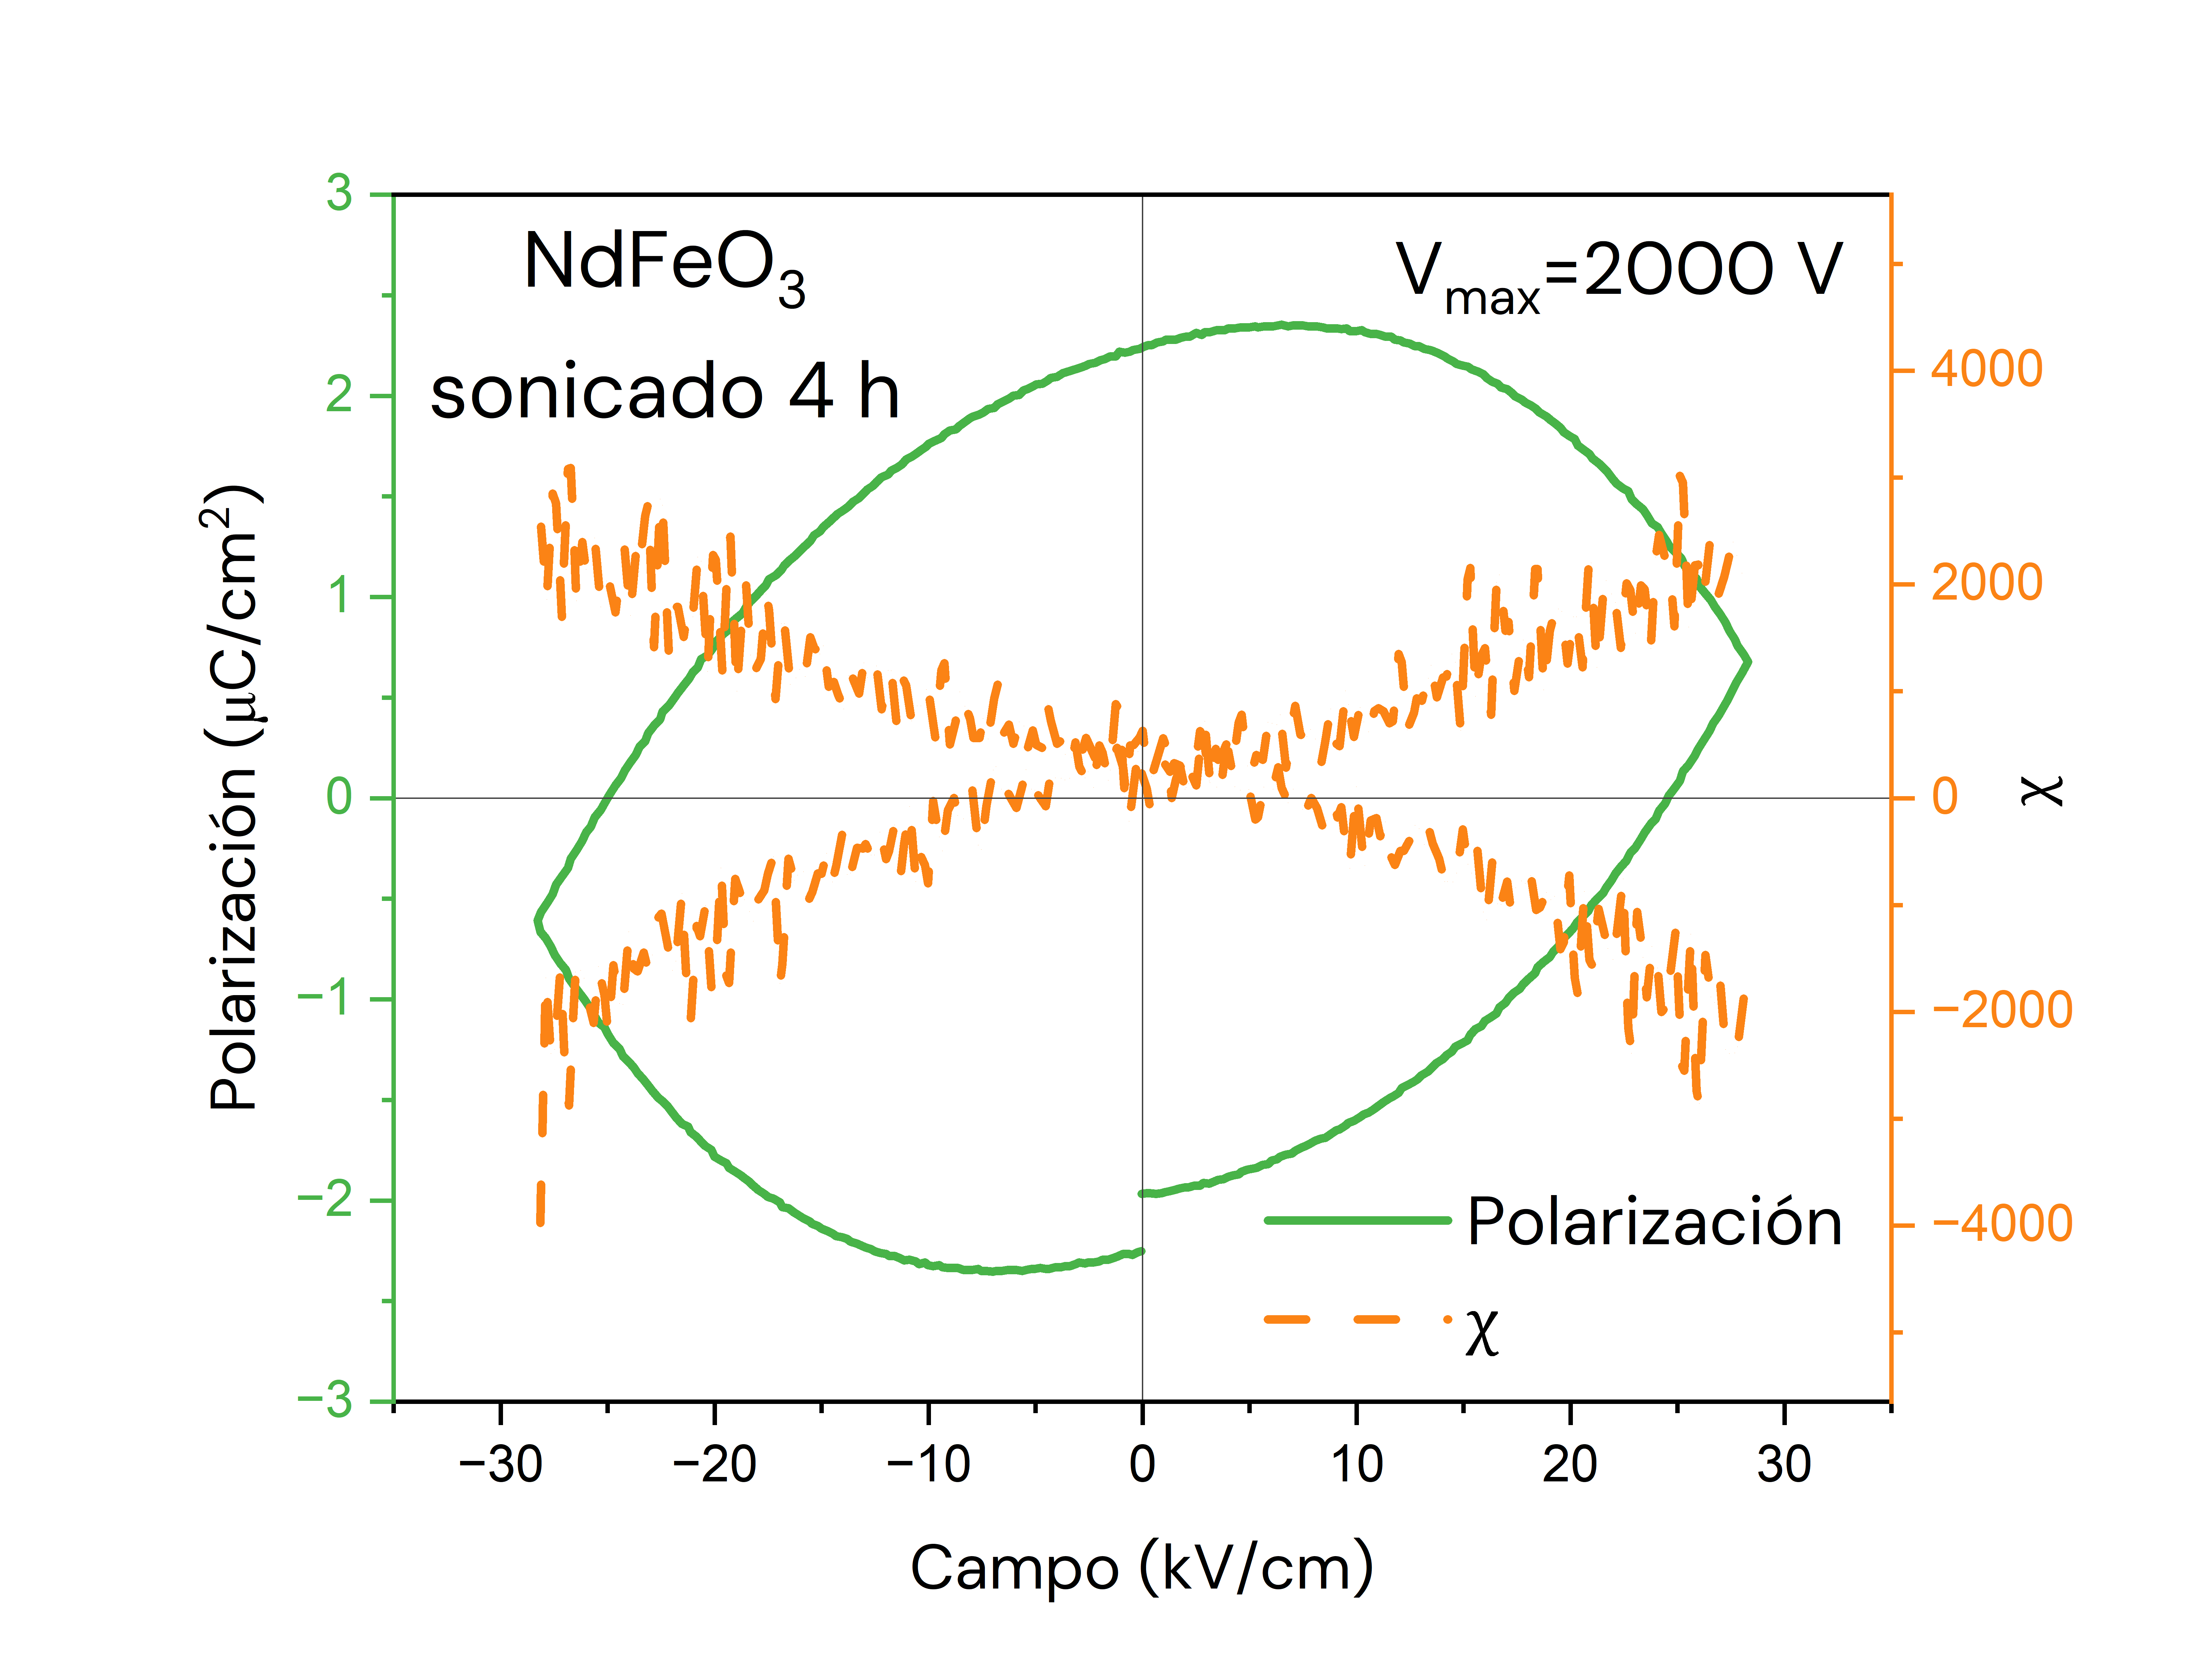
\includegraphics[width=0.45\textwidth]{fig/PENdFeO3-S2000V.png}
    \caption{Curvas $P$ contra $E$ (eje izquierdo) y $\chi$ contra $E$ (eje derecho) con $V_\text{max}=2000$ V de las muestras de \neod{}: a) sin sonicar y b) sonicada 4 h..}
    \label{fig:nd2000v}
\end{figure}
Se puede observar un comportamiento de histéresis débil sólo en las mediciones realizadas a $V_\text{max}=100$ V (figuras \ref{fig:nd100v} a) y b)), lo cual indica un comportamiento de ferroelectricidad débil. La polarización tiende a un comportamiento dependiente de la corriente similar al de un resistor al aumentar el voltaje, esto es de esperarse pues las muestras son semiconductores, por lo cual, al aplicar un campo eléctrico más grande, los electrones de valencia pueden recibir suficiente energía para saltar a la banda de conducción.

En la tabla \ref{tabla:respolarneod} se reportan los valores obtenidos para $P_r$, $P_s$ y $E_c$ para las mediciones con $V_\text{max}=100$ V de las muestras de \neod{}.

\begin{table}[H]
    \centering
    \begin{tabular}{|c||c|c|c|}
        \hline
        Muestra & $P_s$ ($\mu$C/cm$^2$) & $P_r$ ($\mu$C/cm$^2$) & $E_c$ (kV/cm) \\
        \hline\hline
        \neod{} sin sonicar & 0.0067 $\pm$ 0.00036 & $0.0054 \pm 0.00012$ & $0.7448 \pm 0.01392$ \\
        \hline
        \neod{} sonicada & 0.0062 $\pm$ 0.00018 & $0.0044 \pm 0.00017$ & $0.6651 \pm 0.08038$ \\
        \hline
        \end{tabular} 
    \caption{Valores de $P_r$, $P_s$ y $E_c$ medidos de las muestras de \neod{} sin sonicar y sonicada 4 h.}
    \label{tabla:respolarneod}
\end{table}
\subsection{\texorpdfstring{\sama{}}{SmFeO3}}
\subsubsection{Espectroscopía UV-Vis}
De manera análoga a las muestras de \neod{}, se obtuvieron los siguientes resultados para las de \sama{} (figura \ref{fig:absorbressama}):
\begin{figure}[H]
    \centering
    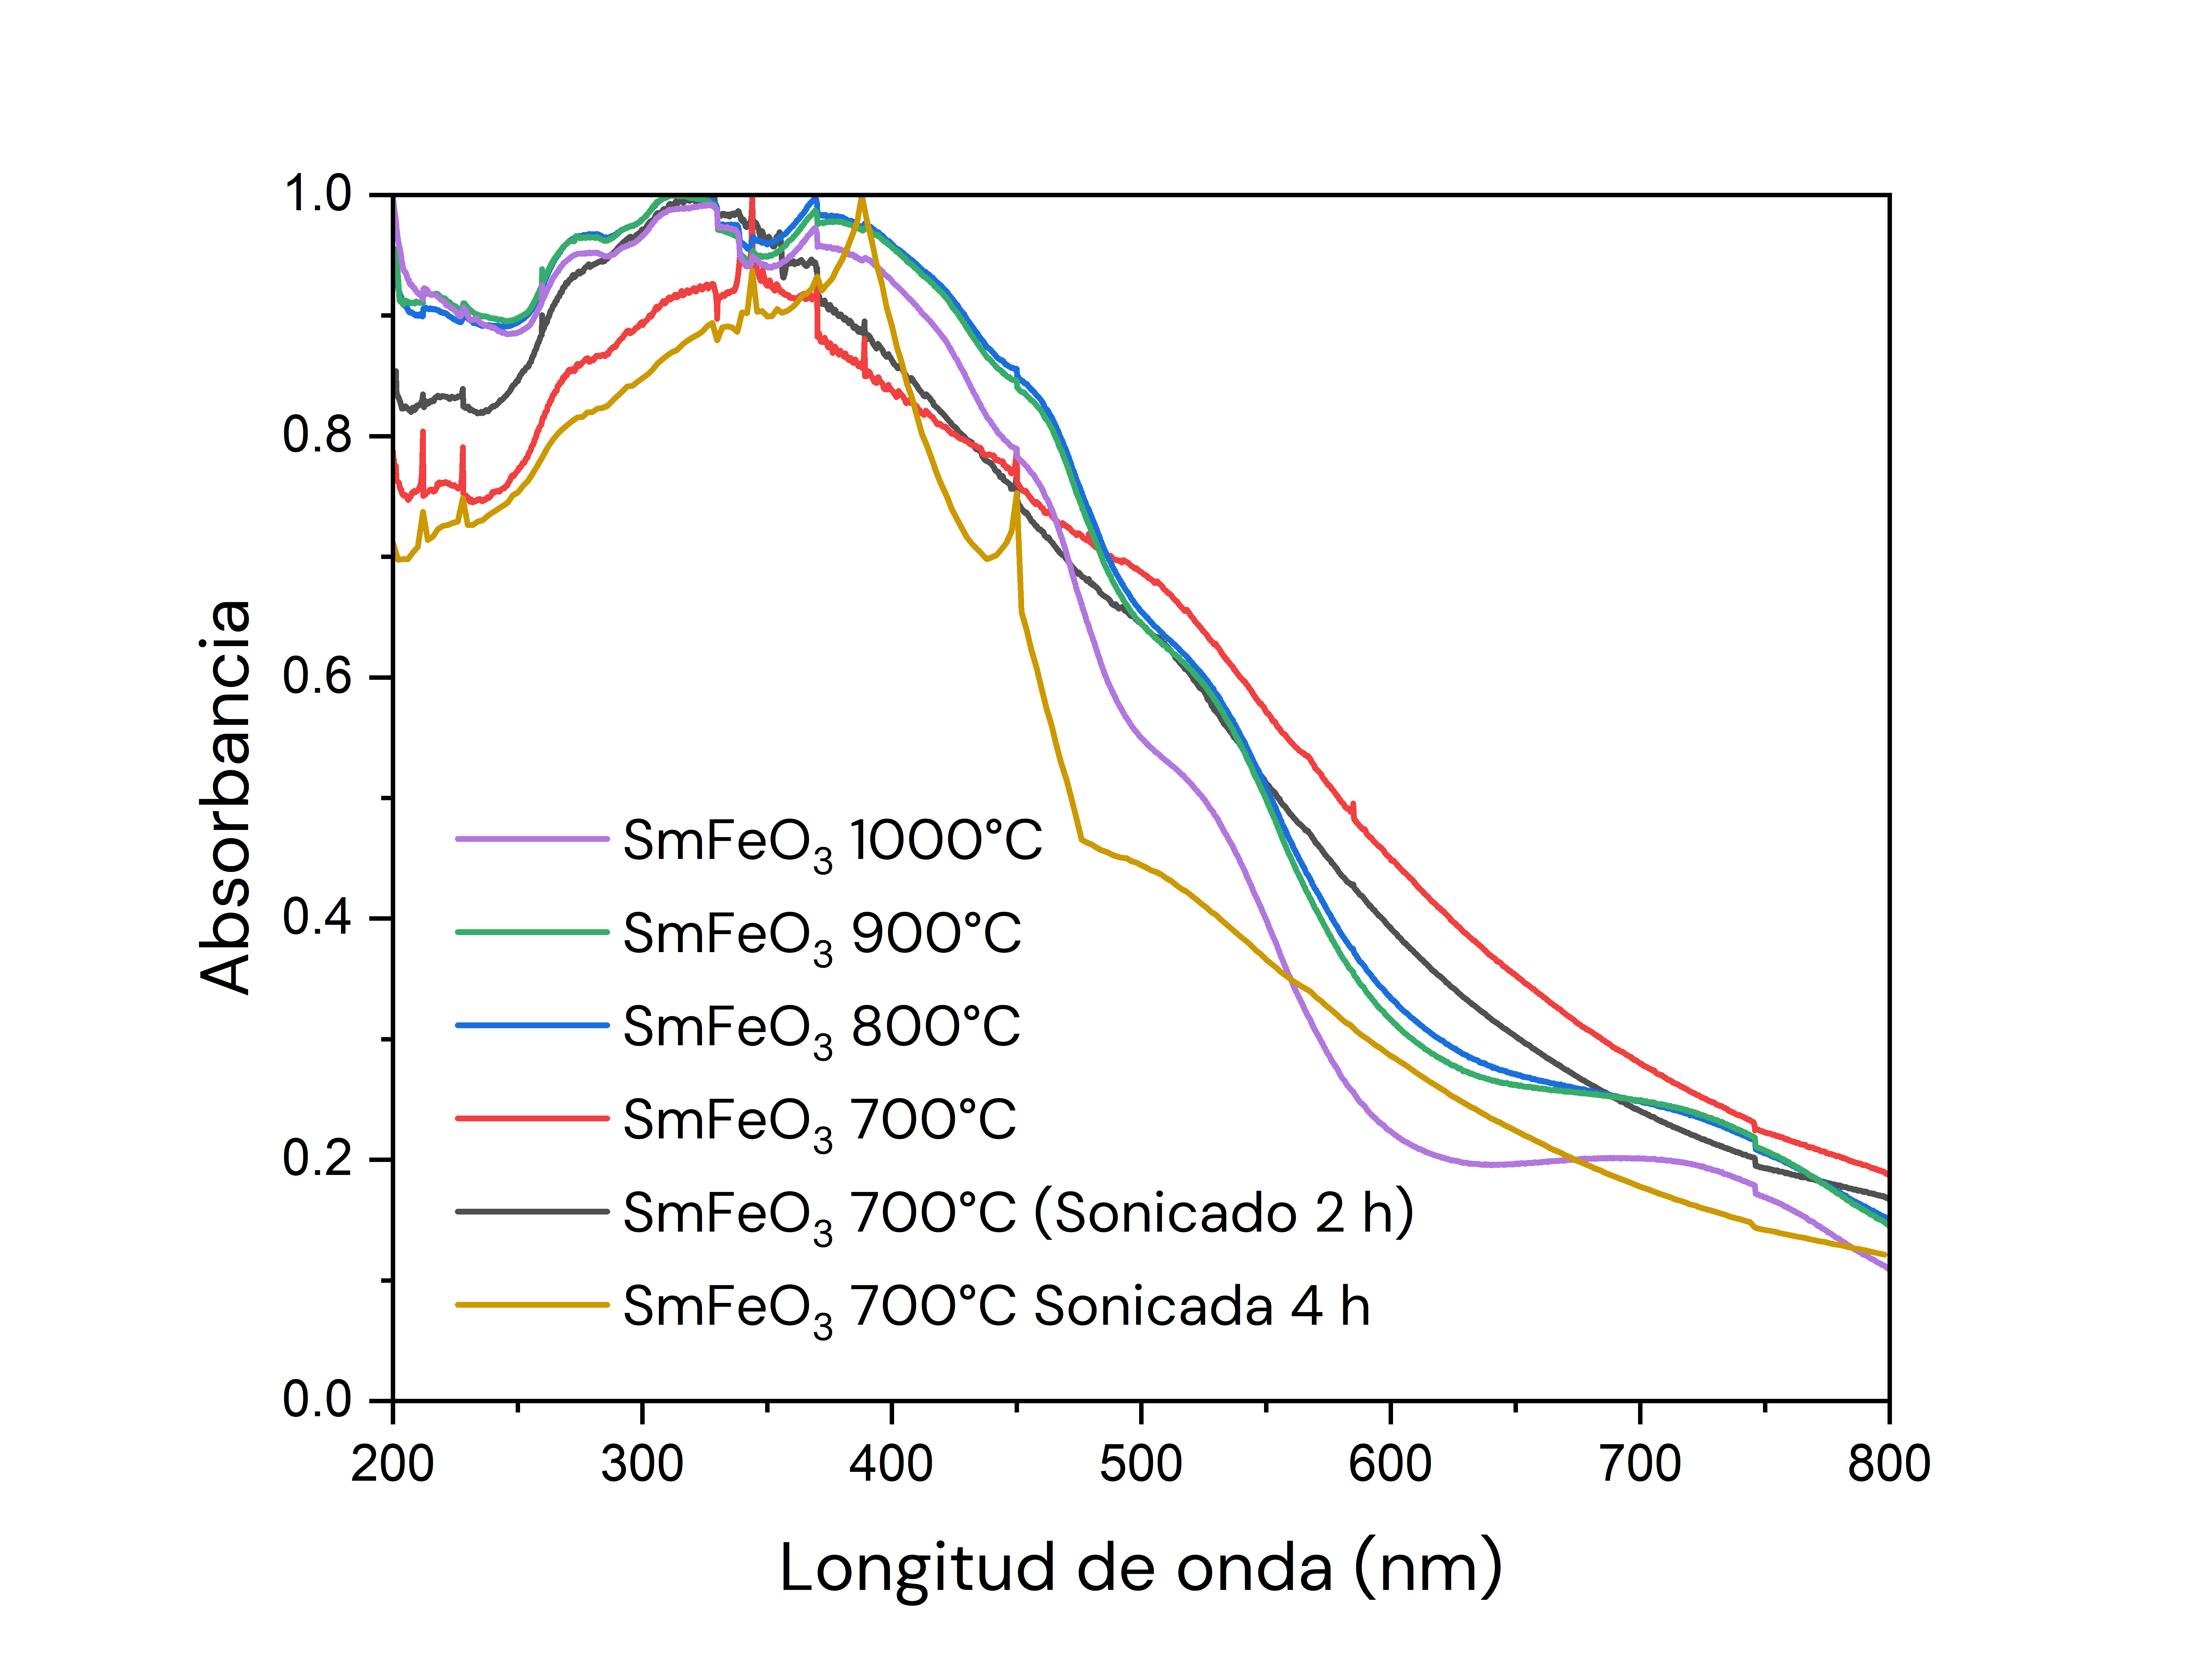
\includegraphics[width=0.7\textwidth]{fig/absorbanciasama.png}
    \caption{Gráficas de la absorbancia contra la longitud de onda para las muestras de \sama{}.}
    \label{fig:absorbressama}
\end{figure}
Aplicando el método Tauc igualmente se obtuvieron los \textit{band gaps} reportados en la tabla \ref{tabla:bandgapssama}
\begin{table}[H]
    \centering
    \begin{tabular}{|c||c|c|}
        \hline
        Muestra & Temperatura de & \textit{Band Gap} \\
        & calcinación & (eV) \\
        \hline\hline
        \multirow{6}{*}{\rotatebox[origin=c]{90}{\sama{}}} & 700\gradoC{} & 2.03$\pm$0.002 \\
        \cline{2-3}
        & 700\gradoC{}, sonicada 2 h & 2.14$\pm$0.015 \\
        \cline{2-3}
        & 700\gradoC{}, sonicada 4 h & 2.22$\pm$0.002 \\
        \cline{2-3}
        & 800\gradoC{} & 2.20$\pm$0.001 \\
        \cline{2-3}
        & 900\gradoC{} & 2.21$\pm$0.001 \\
        \cline{2-3}
        & 1000\gradoC{} & 2.30$\pm$0.001 \\
        \hline
    \end{tabular} 
    \caption{\textit{Band gaps} de las distintas muestras según su temperatura de calcinación.}
    \label{tabla:bandgapssama}
\end{table}
\begin{figure}[H]
    \centering
    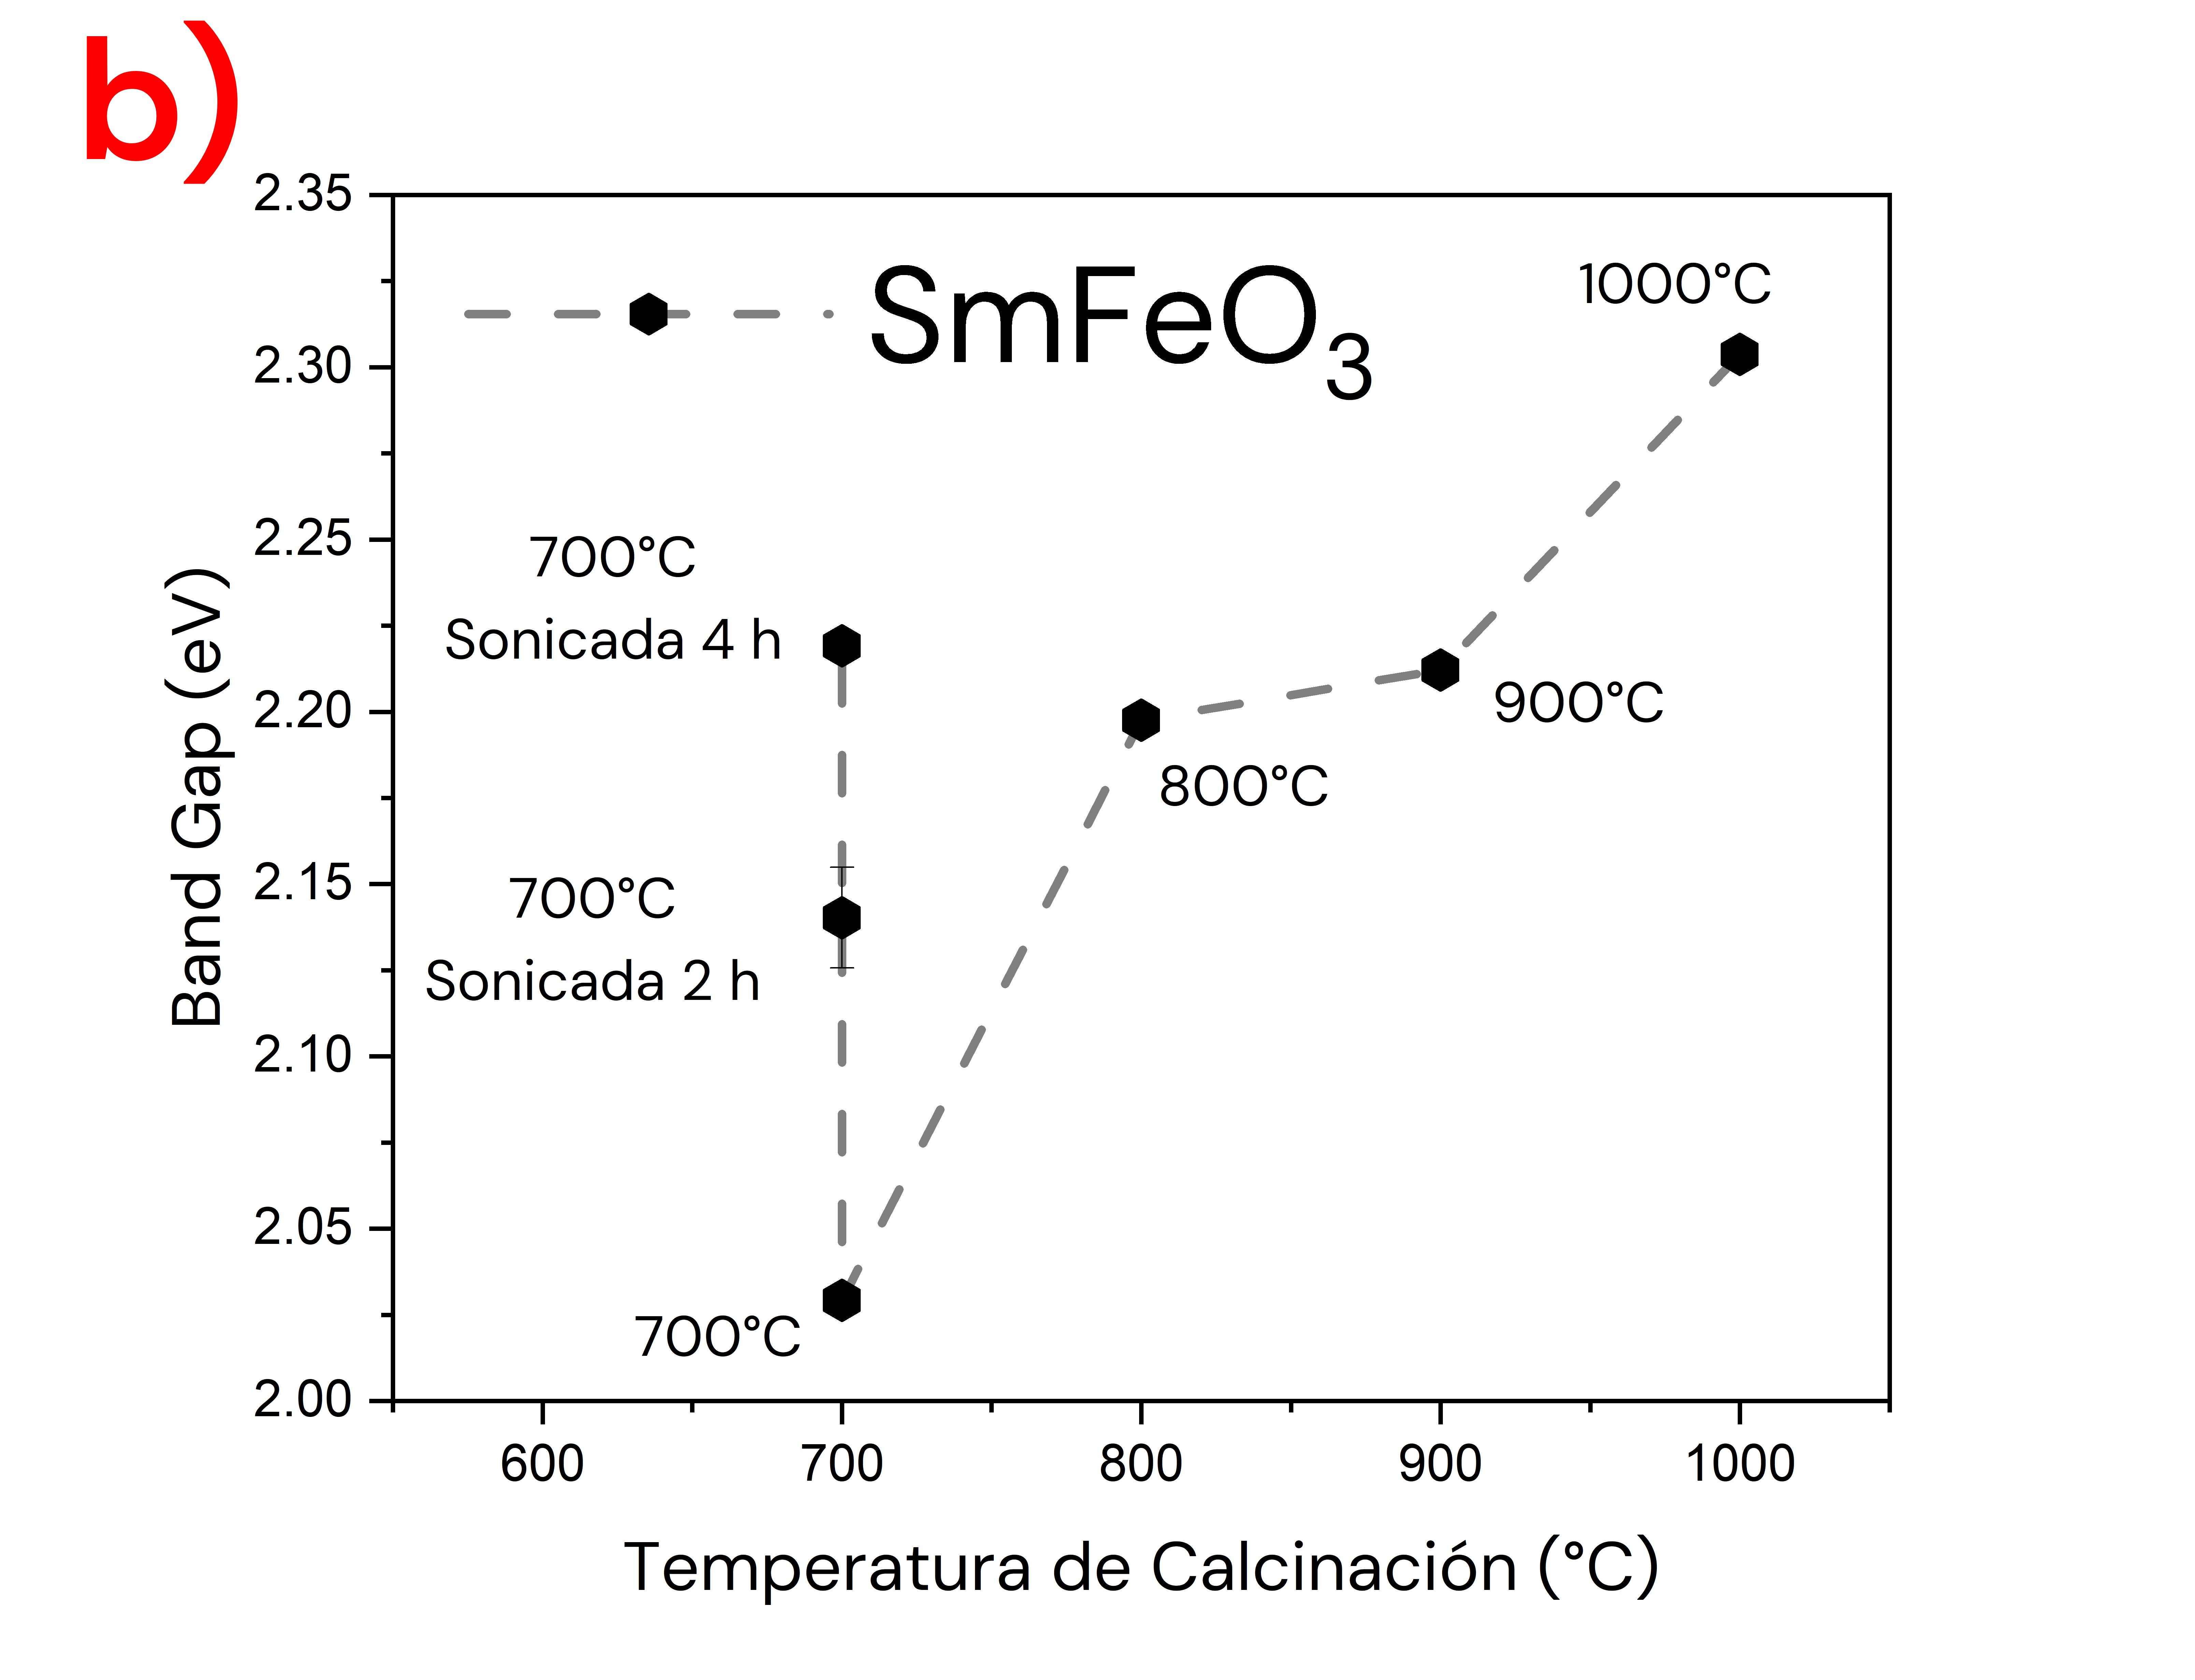
\includegraphics[width=0.7\textwidth]{fig/BGSmFeO3.png}
    \caption{Gráfica del \textit{band gap} de cada muestra de \sama{} según su temperatura de calcinación.}
    \label{fig:bandgapvT}
\end{figure}
En este caso también se observa que el \textit{band gap} aumenta con la temperatura y el tiempo de sonicación, ocurriendo de la misma forma un mínimo en la muestra calcinada a menor temperatura y sin sonicar.
\subsubsection{Magnetometría SQUID}
Se obtuvieron las siguientes curvas de $M$ vs $H$
\begin{figure}[H]
    \centering
    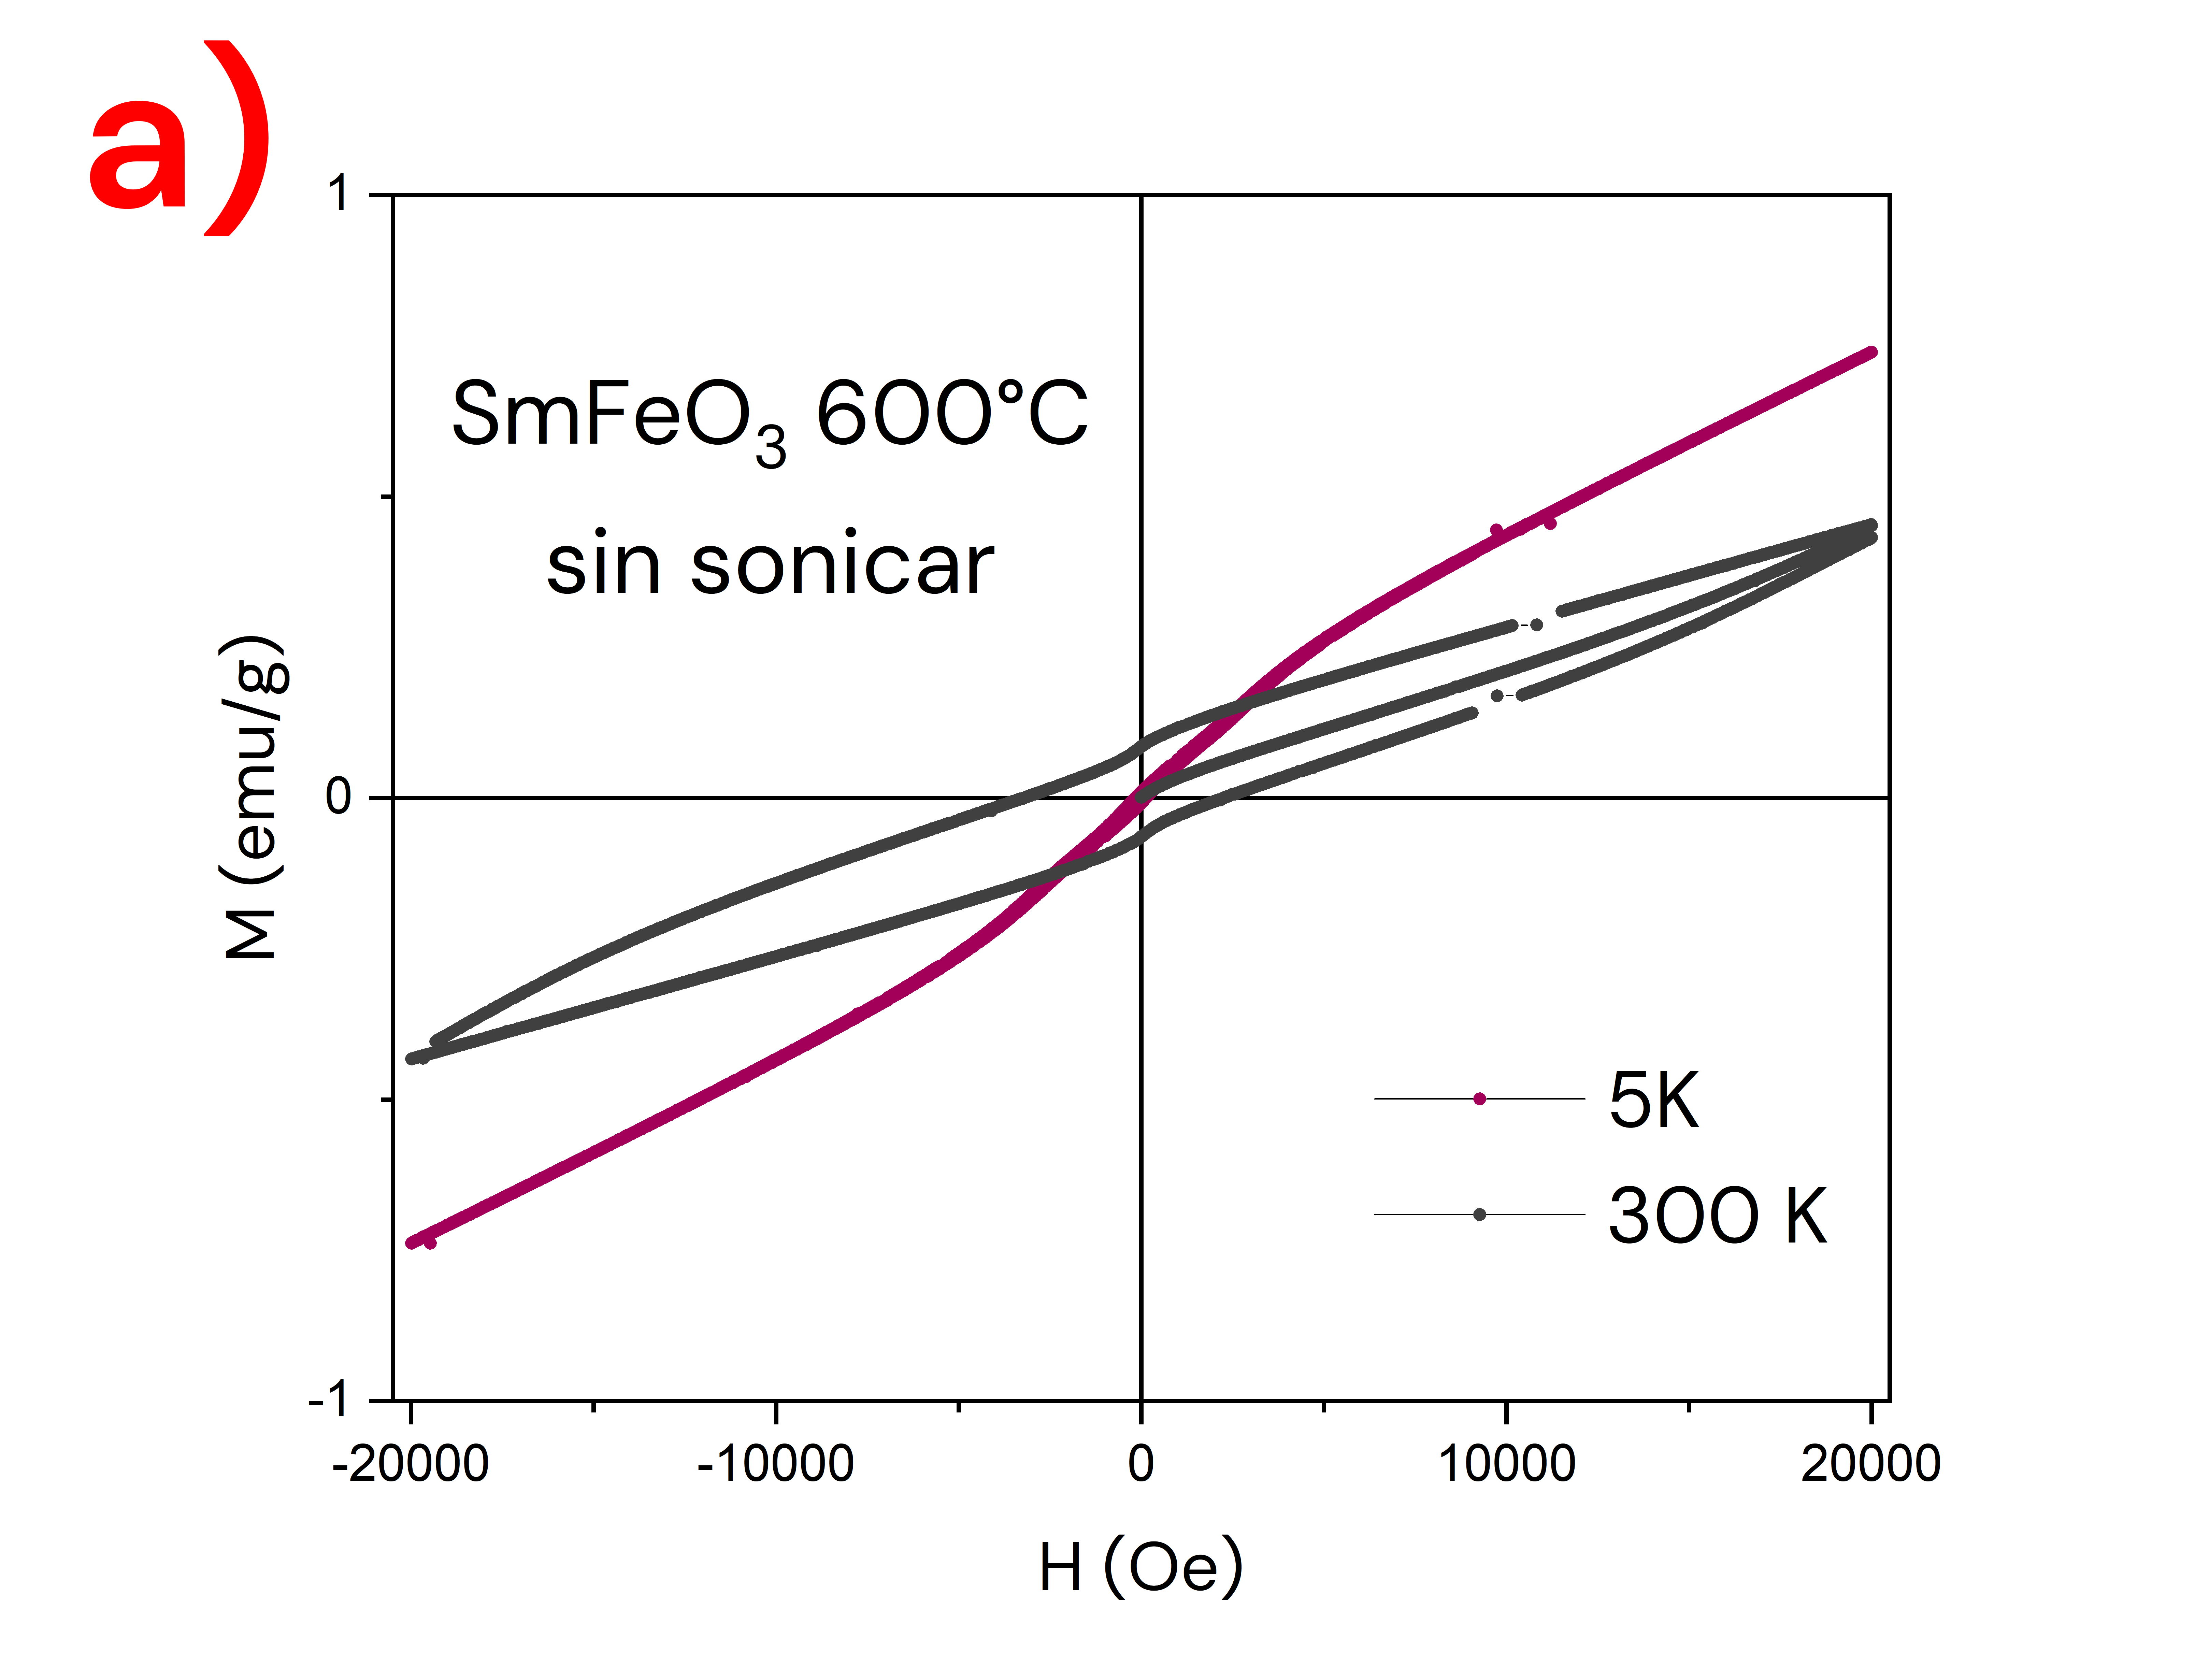
\includegraphics[width=0.45\textwidth]{fig/mvhSm.png}
    \quad
    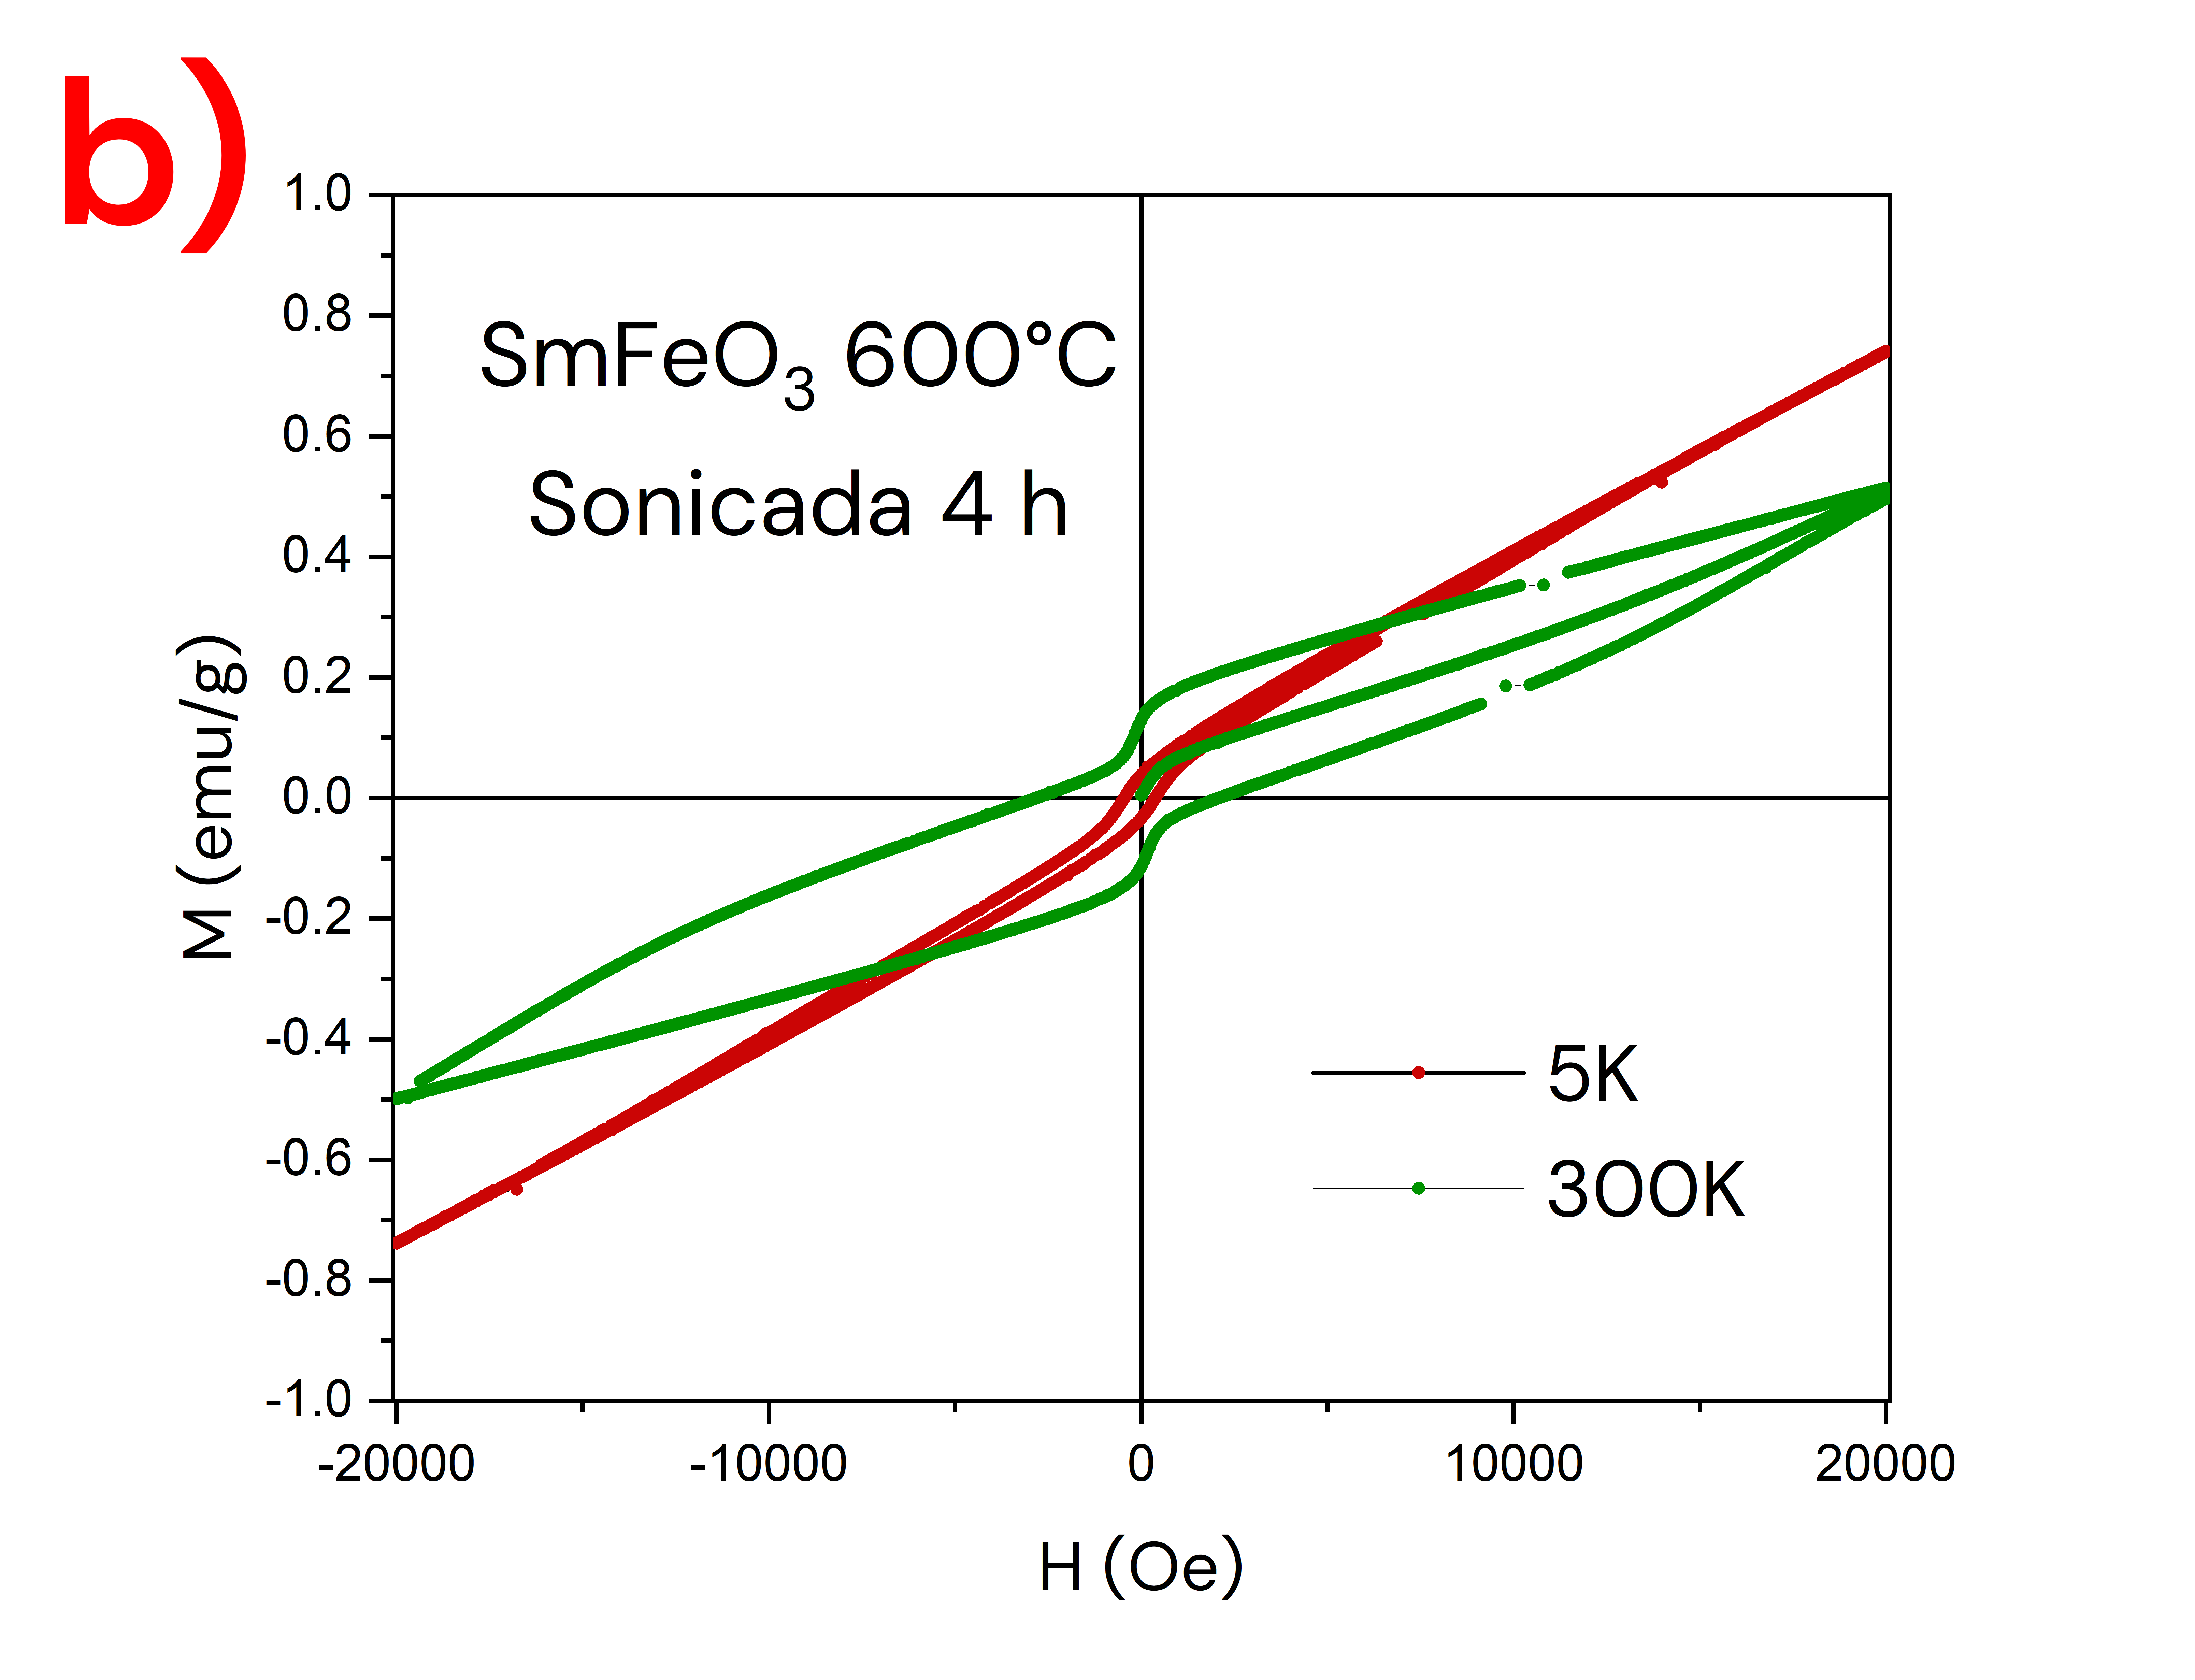
\includegraphics[width=0.45\textwidth]{fig/mvhSm-S.png}
    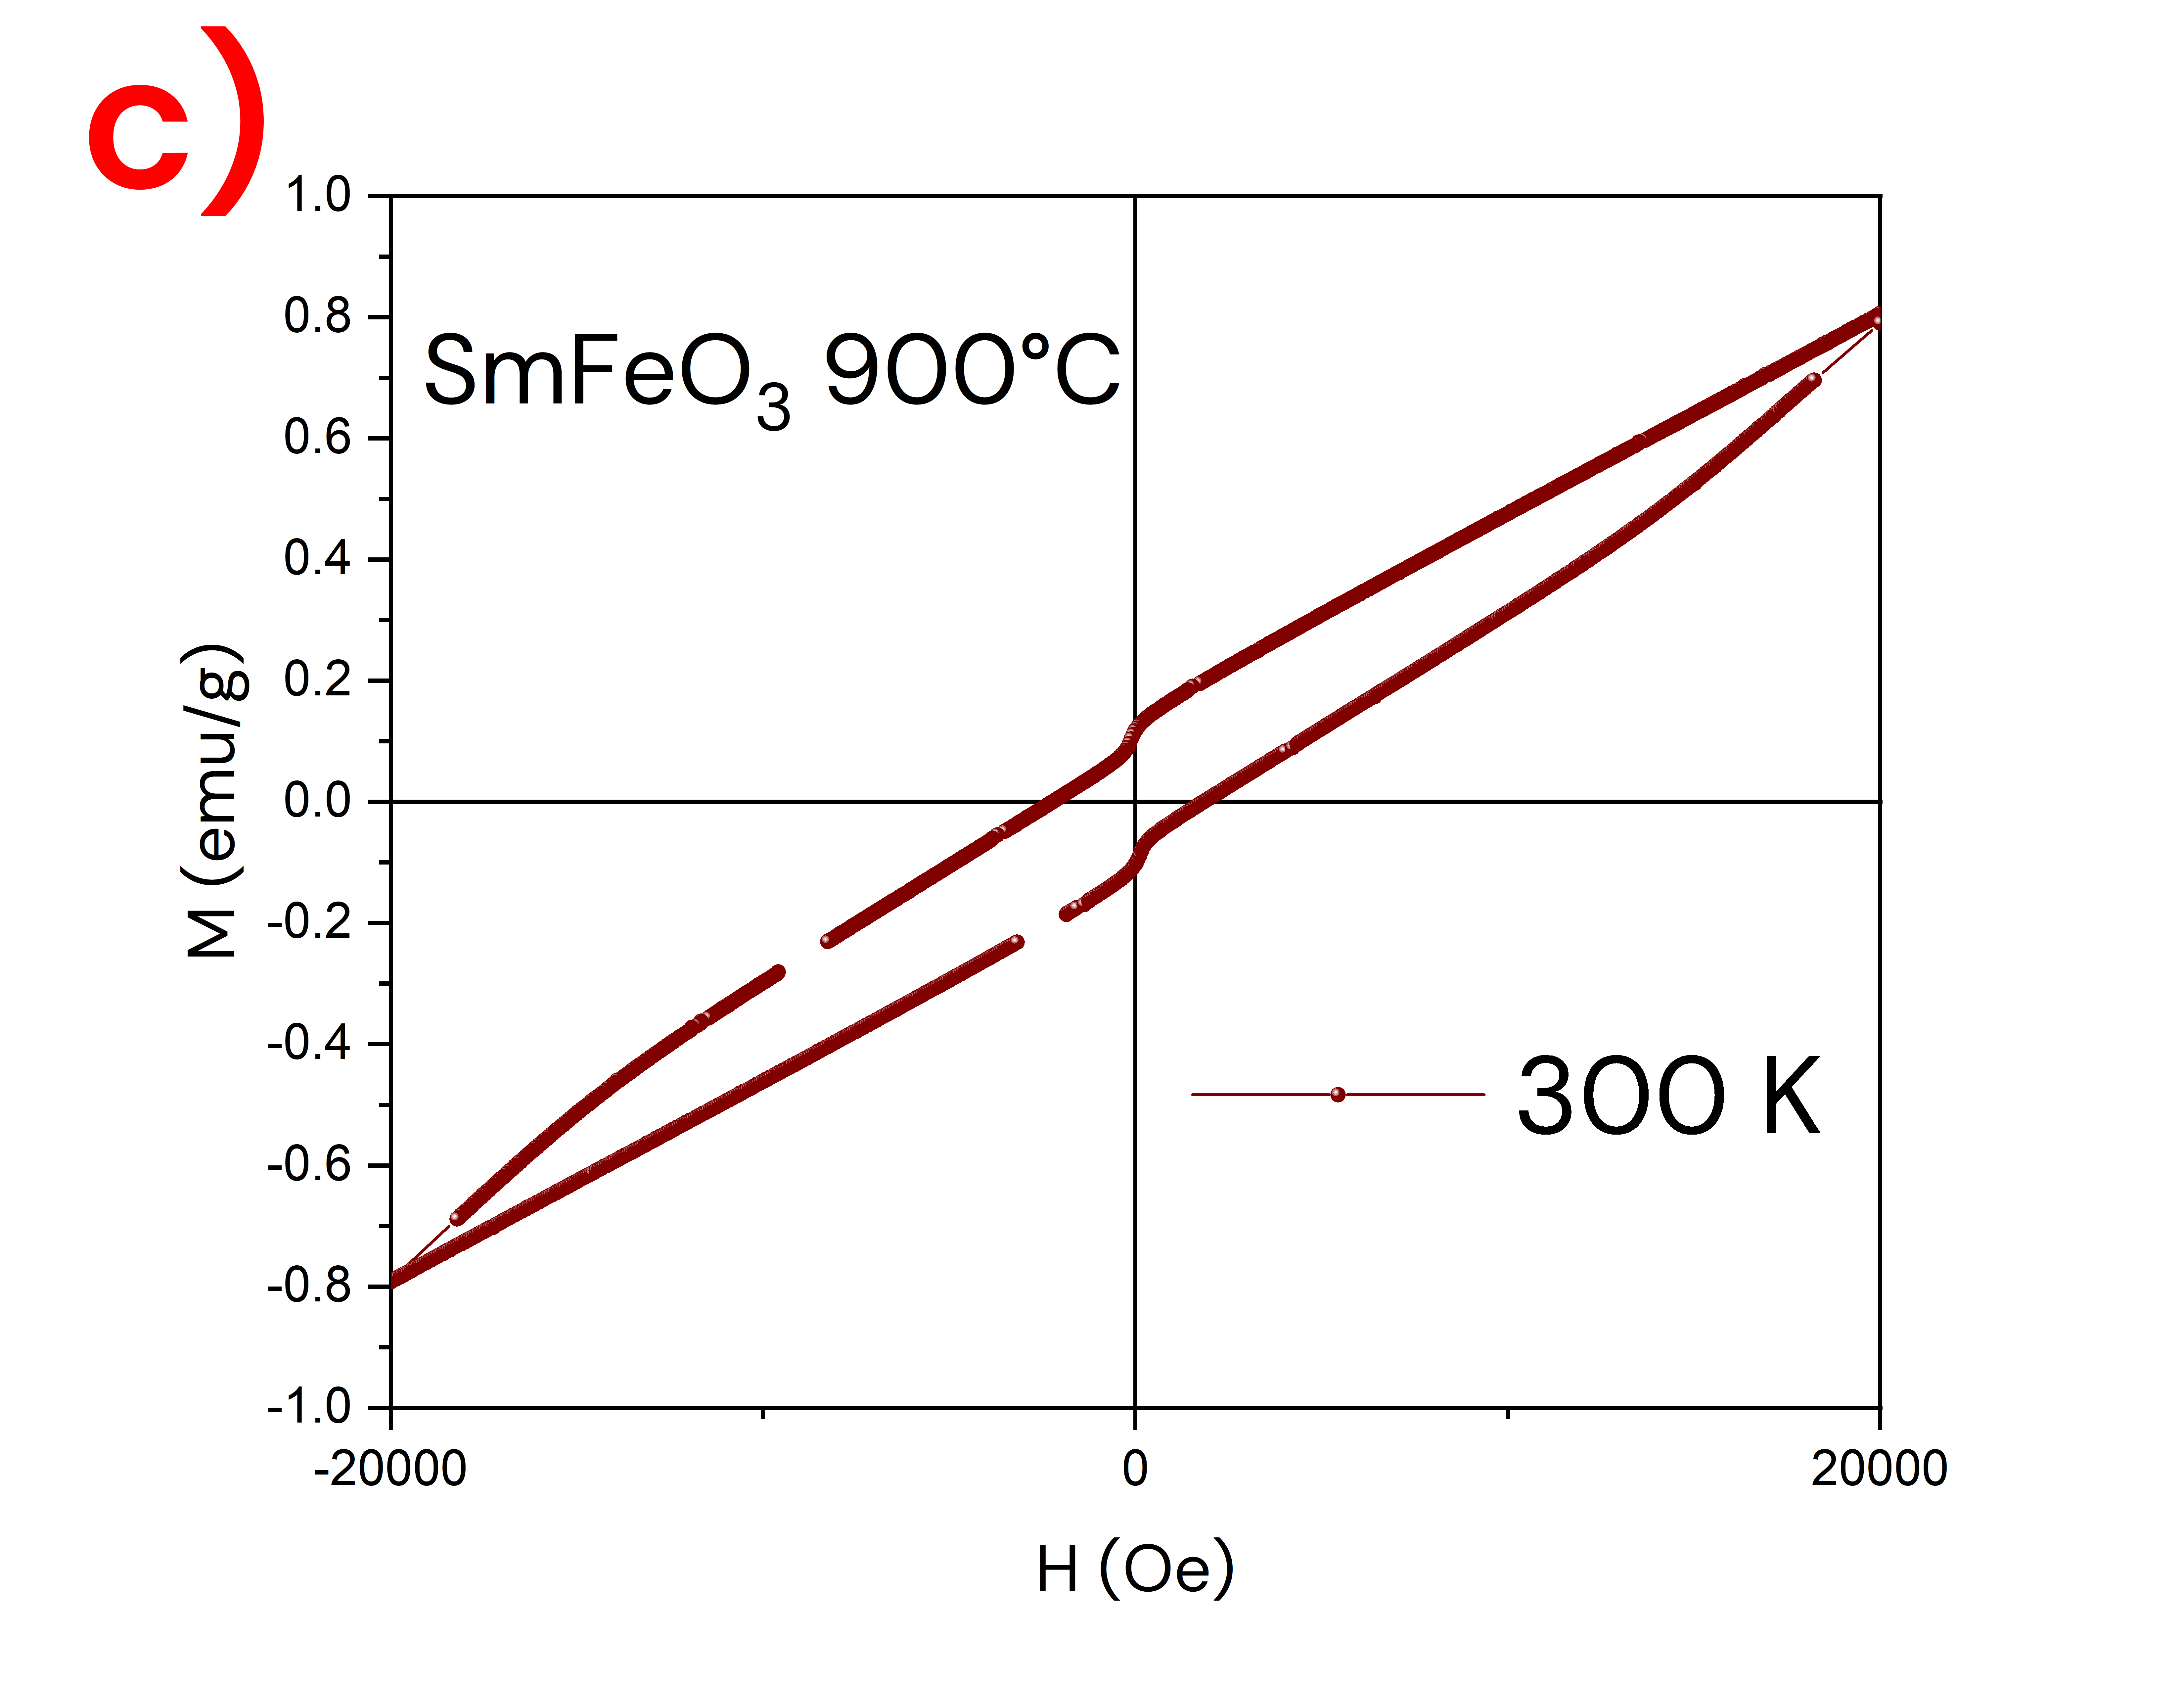
\includegraphics[width=0.45\textwidth]{fig/mvhSm900.png}
    \caption{Curvas $M$ contra $H$ para las muestras de \sama{}: a) calcinada a 600\gradoC{} sin sonicar, b) calcinada a 600\gradoC{} sonicada y c) calcinada a 900\gradoC{}.}
    \label{fig:mvhSm}
\end{figure}
A diferencia del \neod{}, las muestras de \sama{} muestran un comportamiento ferromagnético débil independientemente de la temperatura de calcinación. Se observa que en este caso la sonicación provocó una mejoría en las propiedades ferromagnéticas de la muestra calcinada a 700\gradoC{}, observando incluso un ciclo de histéresis a 5 K.

A continuación se reportan los valores obtenidos para $M_r$, $M_s$ y $H_c$.
\begin{table}[H]
    \centering
    \begin{tabular}{|c||c|c|c|}
        \hline 
        Muestra & $M_s$ (emu/g) & $M_r$ (emu/g) & $H_c$ (Oe) \\
        \hline
        \hline
        \multicolumn{4}{|c|}{$T=5$ K} \\
        \hline 
        \sama{} (700\gradoC{}) sin sonicar & 0.13$\pm$0.002 & 0.01$\pm$0.004 & 252.014$\pm$5.531 \\
        \hline
        \sama{} (700\gradoC{}) sonicada 4 h & 0.04$\pm$0.001 & 0.08$\pm$0.002 & 591.54$\pm$20.834 \\
        \hline
        \multicolumn{4}{|c|}{$T=300$ K} \\
        \hline
        \sama{} (700\gradoC{}) sin sonicar & 0.06$\pm$0.001 & 0.07$\pm$0.001 & 2206.76$\pm$41.575 \\
        \hline
        \sama{} (700\gradoC{}) sonicada 4 h & 0.17$\pm$0.002 & 0.12$\pm$0.001 & 1561.36$\pm$20.612 \\
        \hline
        \sama{} (1000\gradoC{}) & 0.14$\pm$0.001 & 0.11$\pm$0.002 & 1835.08$\pm$37.872 \\
        \hline
        \end{tabular} 
    \caption{Valores de $M_s$, $M_r$ y $H_c$ obtenidos para las muestras de \sama{}.}
    \label{tabla:resmvhsama}
\end{table}
Por otra parte, se obtuvieron las siguientes curvas $M$ vs $T$ y $\chi$ vs $T$:
\begin{figure}[H]
    \centering
    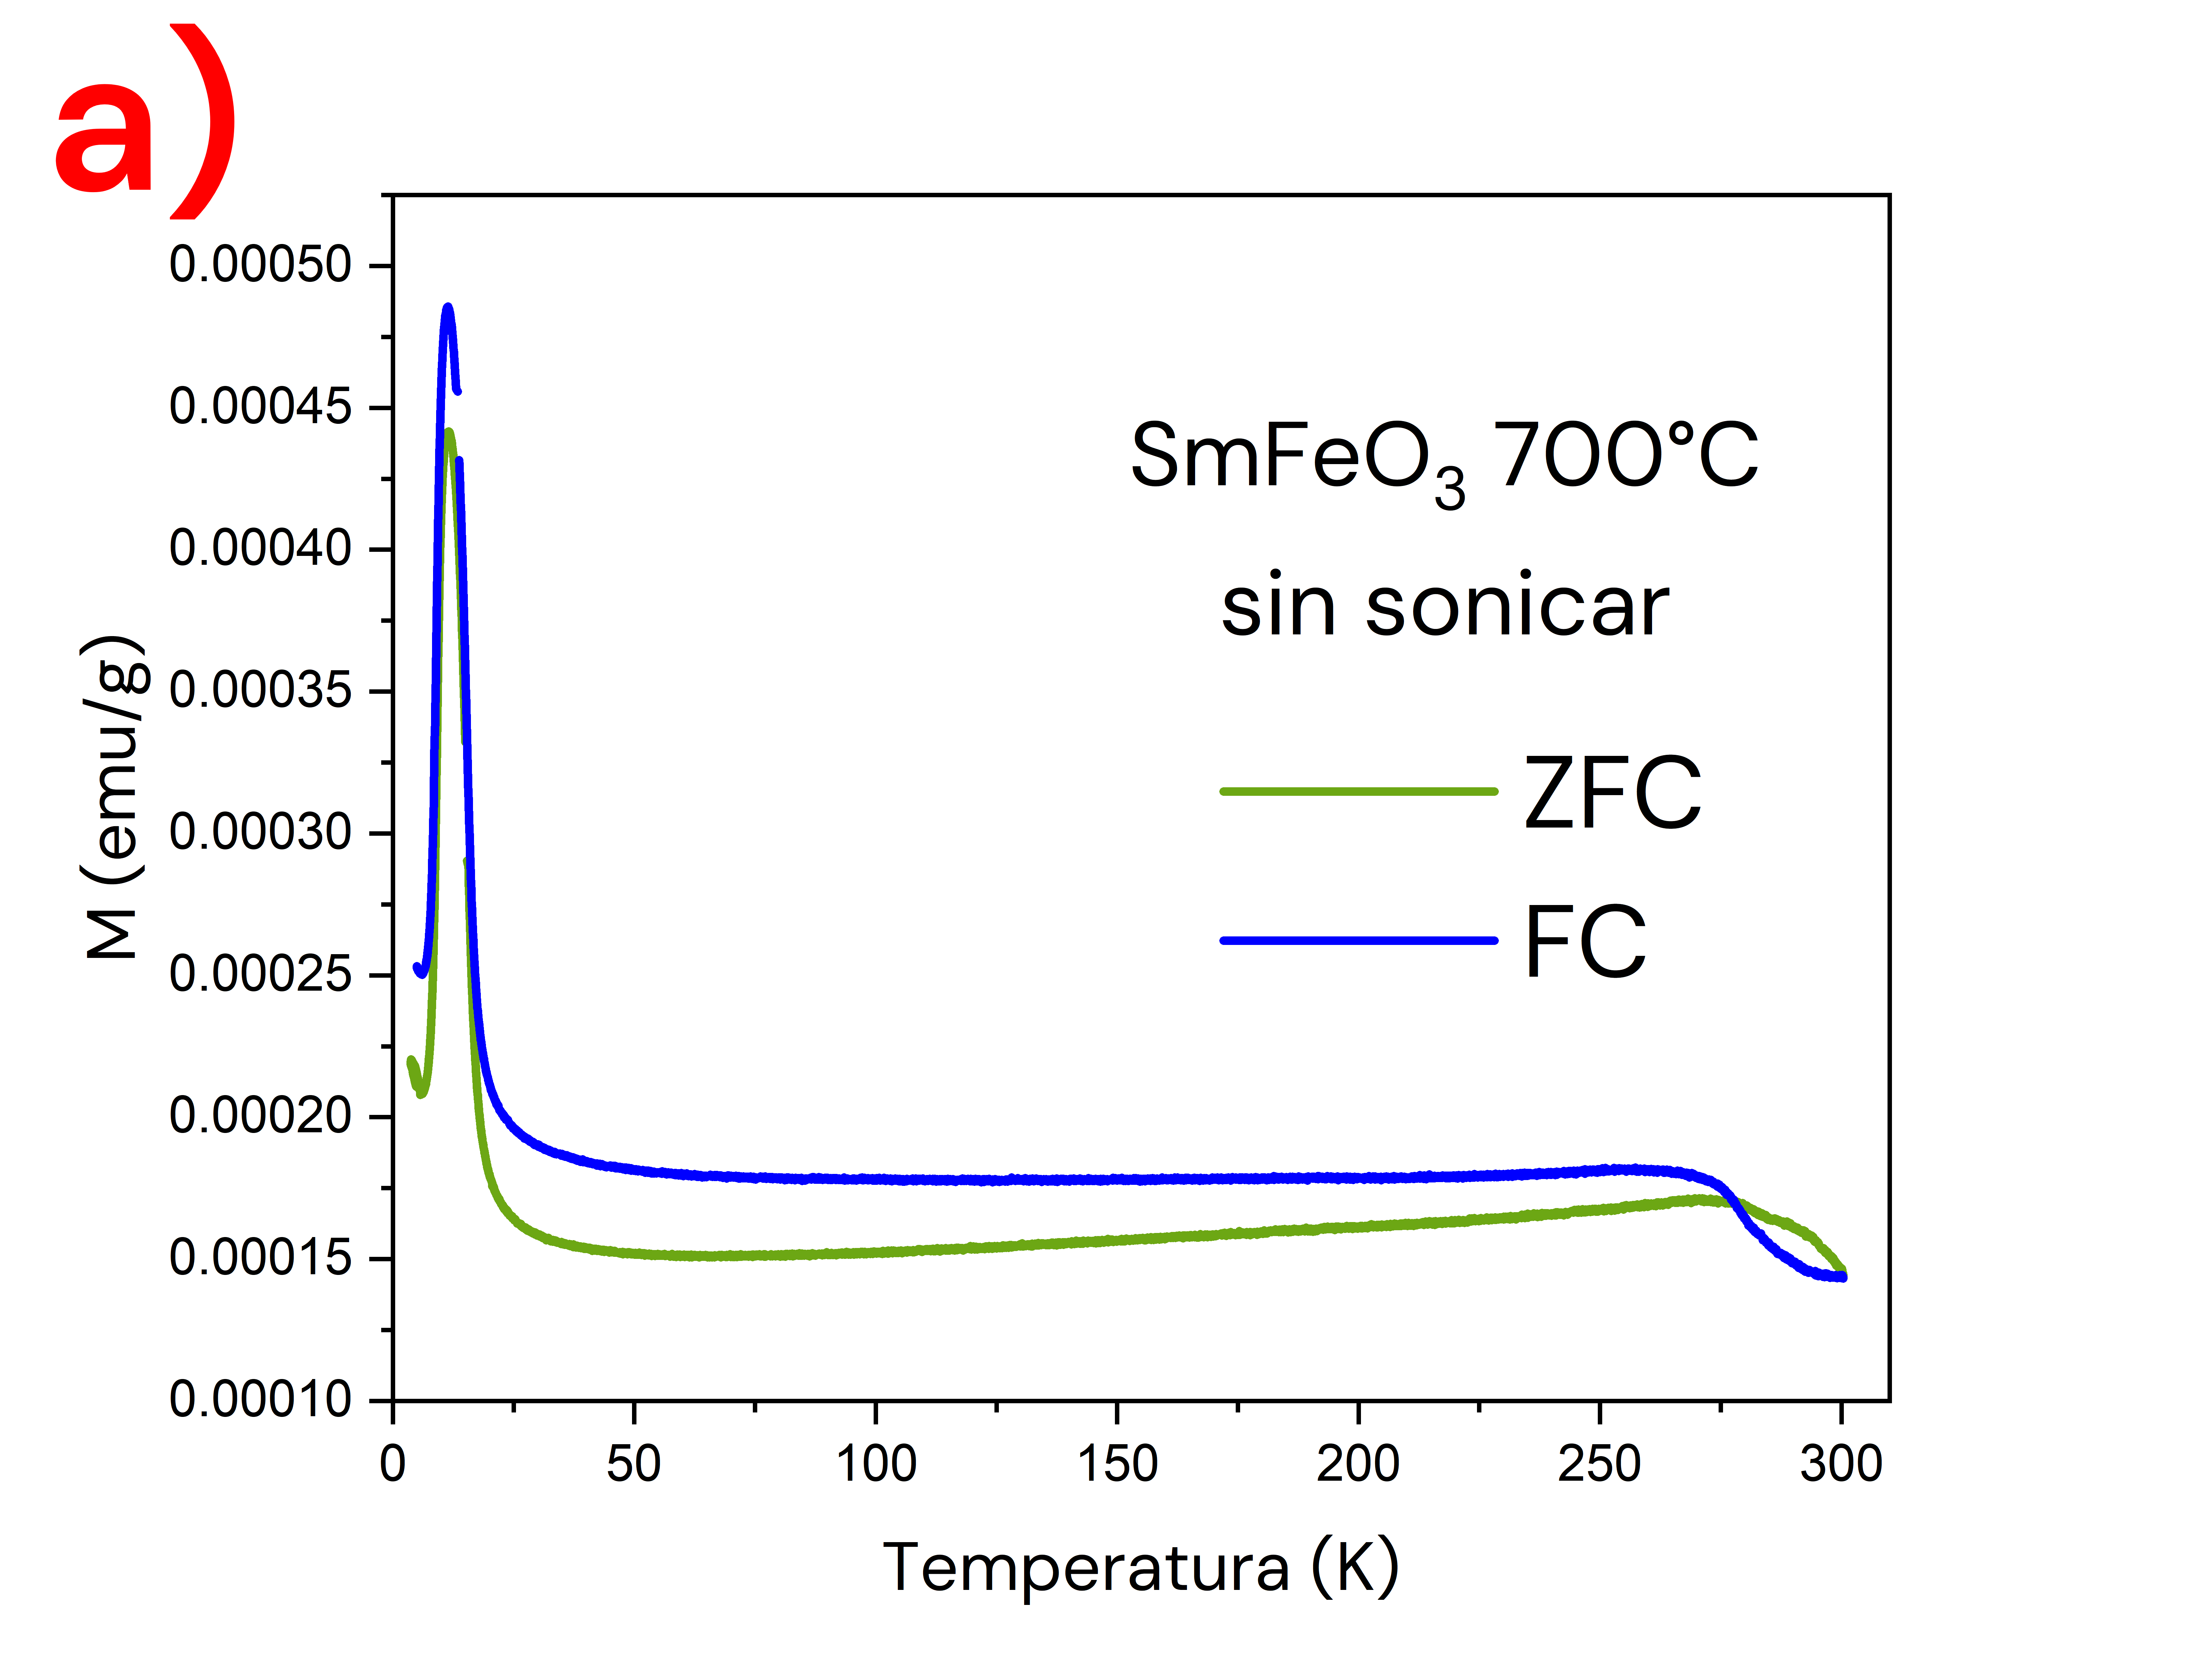
\includegraphics[width=0.45\textwidth]{fig/MvTSm.png}
    \quad
    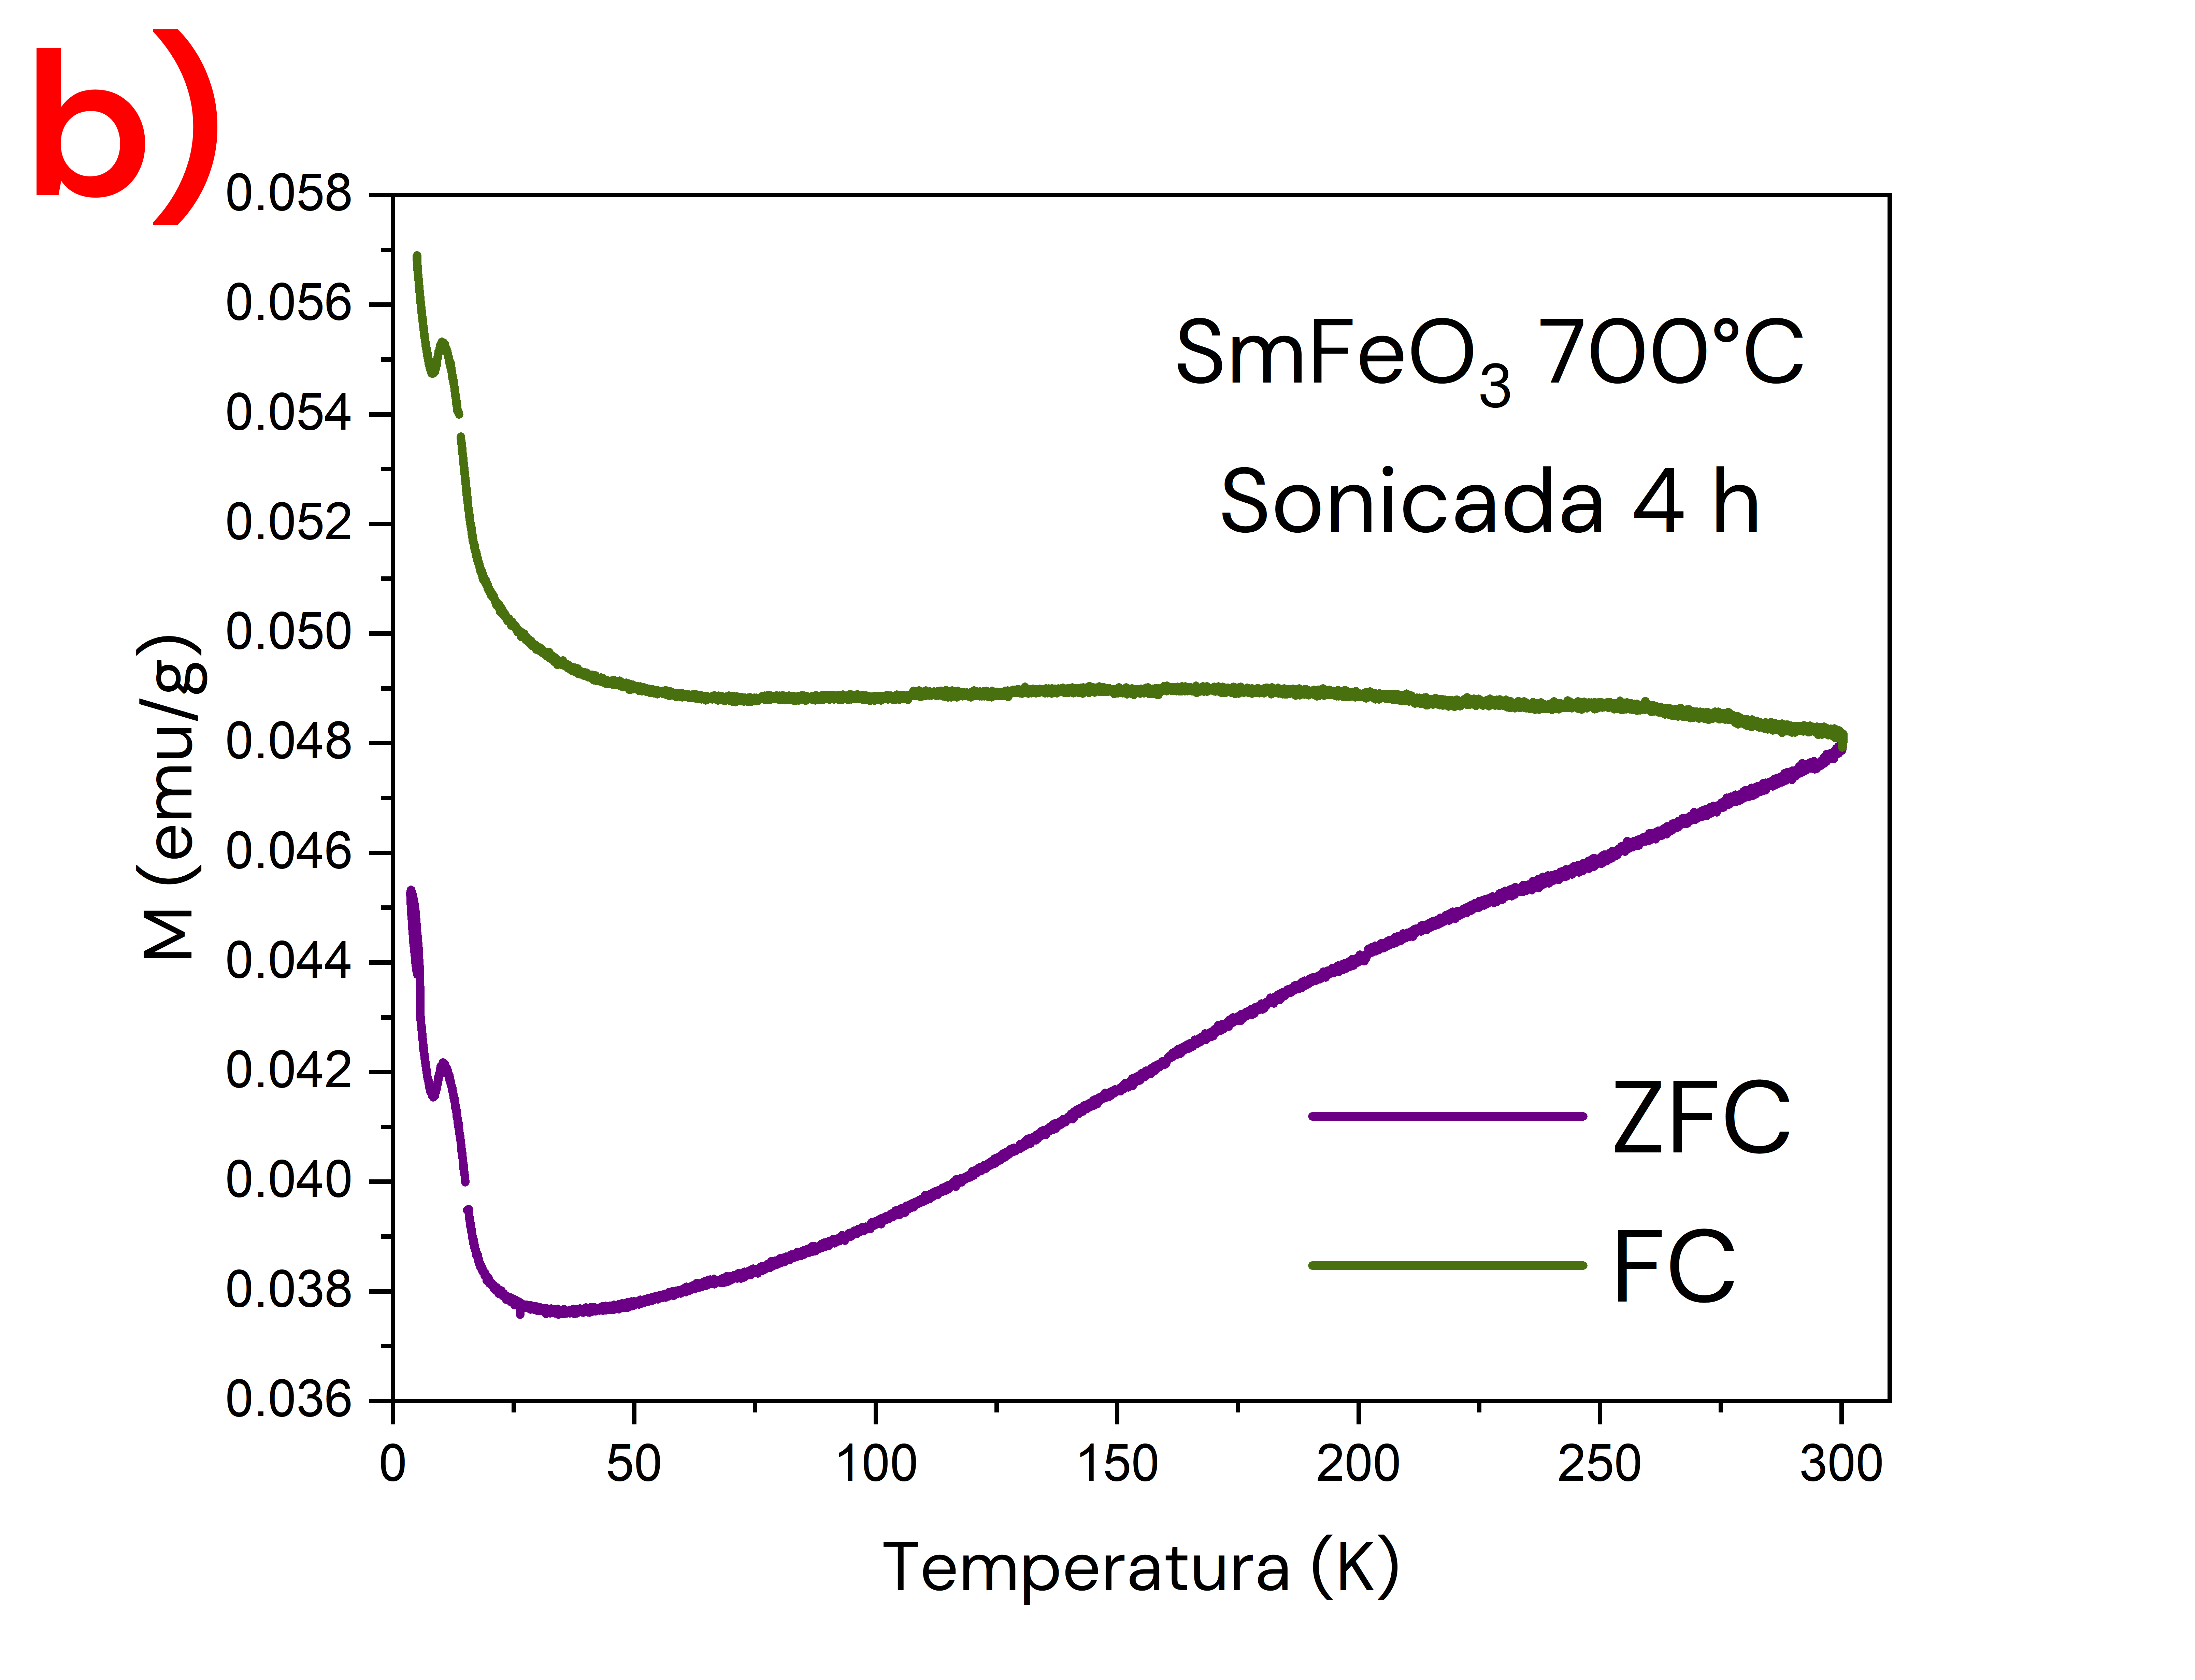
\includegraphics[width=0.45\textwidth]{fig/MvTSm-S.png}
    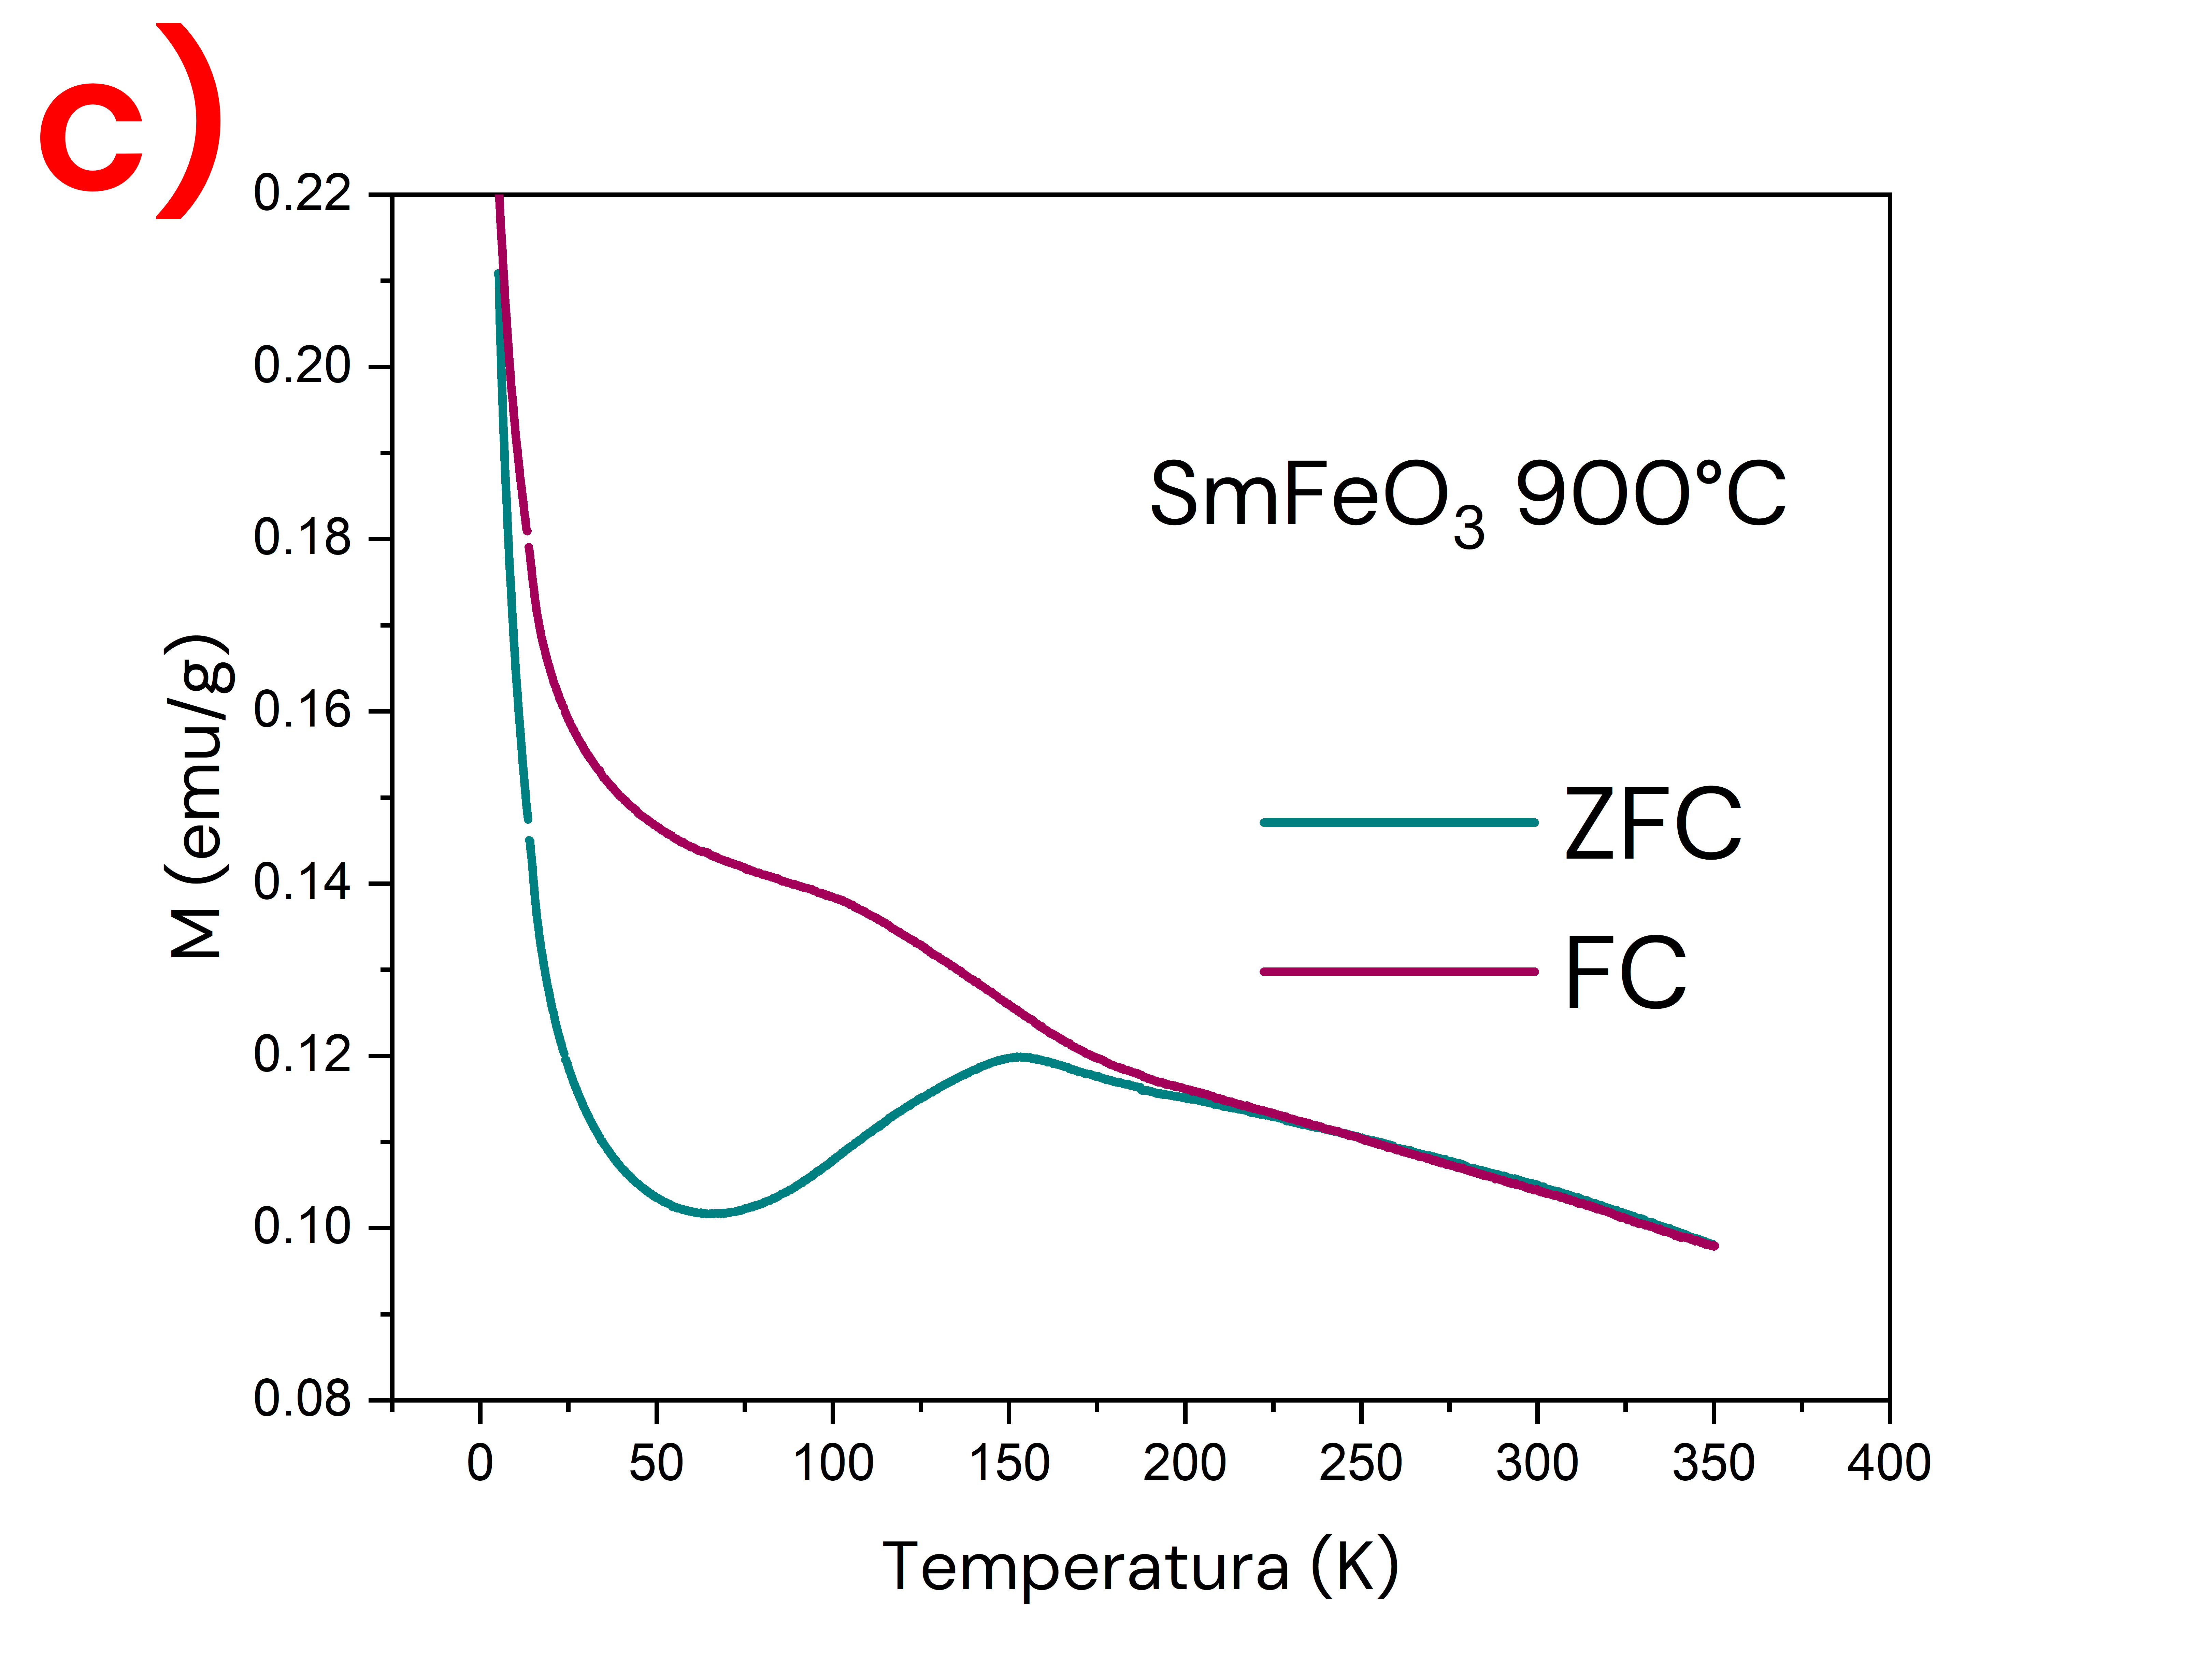
\includegraphics[width=0.45\textwidth]{fig/MvTSm900.png}
    \caption{Curvas $M$ contra $T$ para las muestras de \sama{}: a) sin sonicar y b) sonicada.}
    \label{fig:MvTSm}
\end{figure}
\begin{figure}[H]
    \centering
    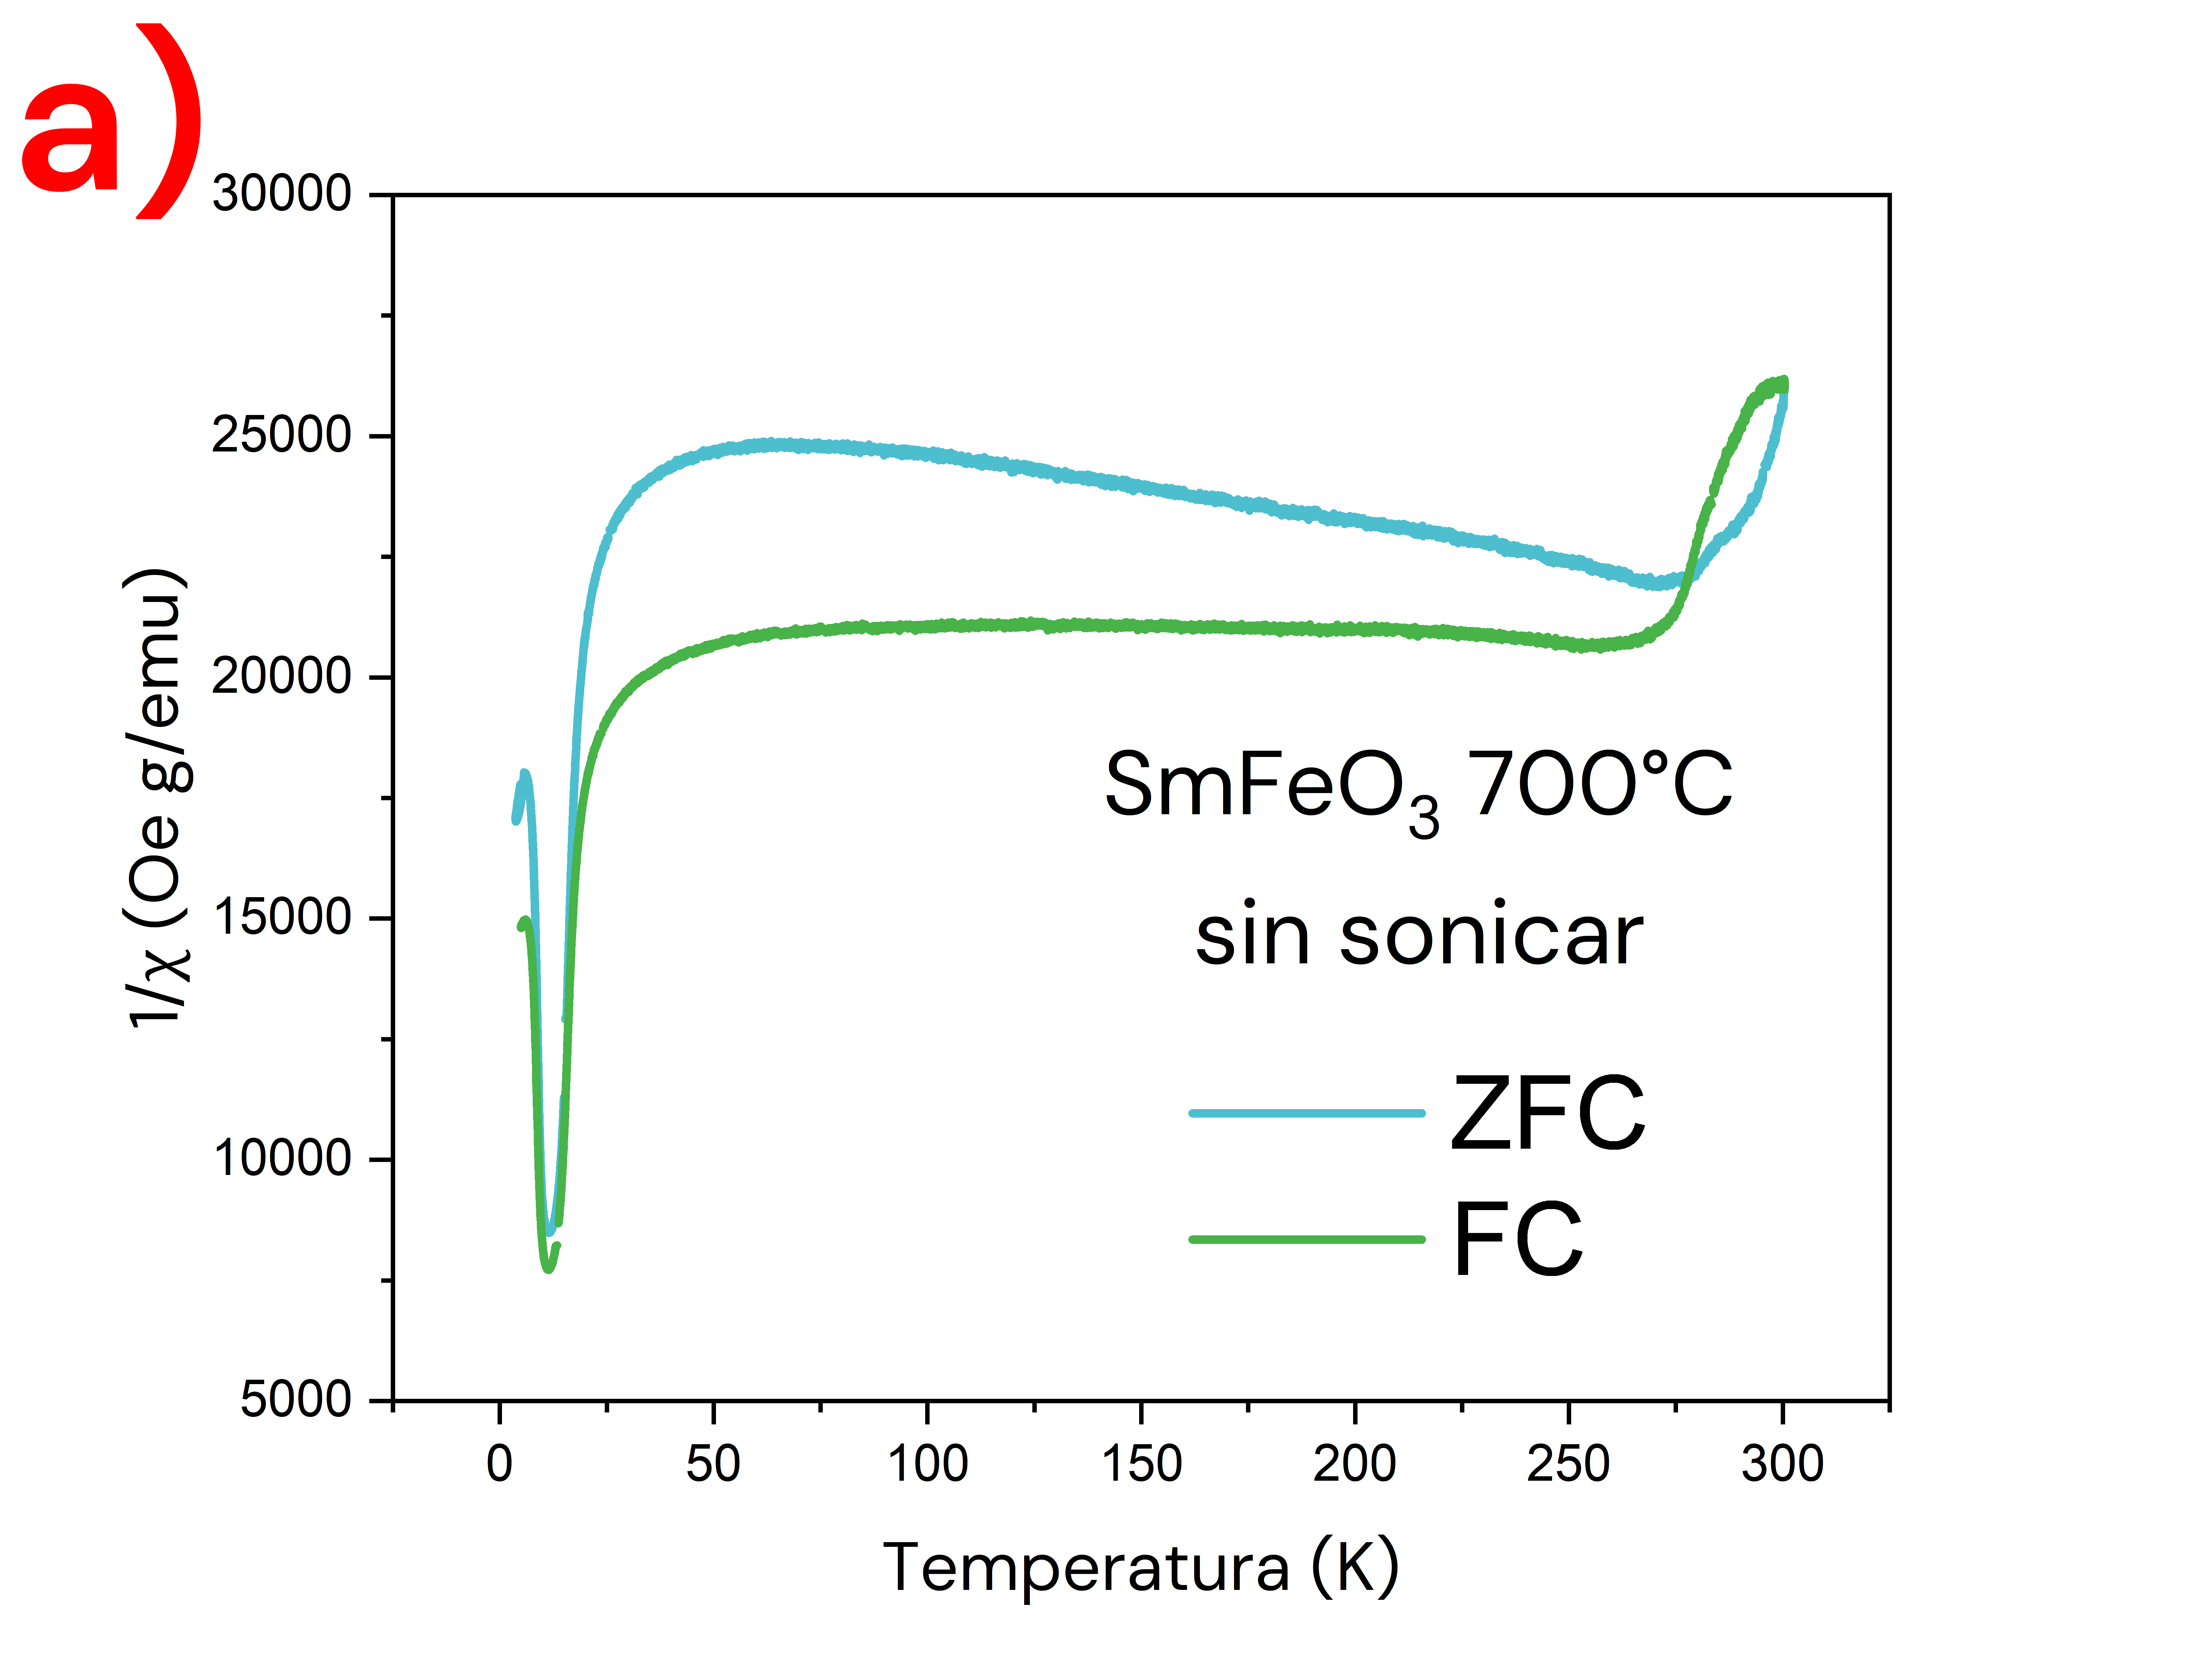
\includegraphics[width=0.45\textwidth]{fig/chivTSm.png}
    \quad
    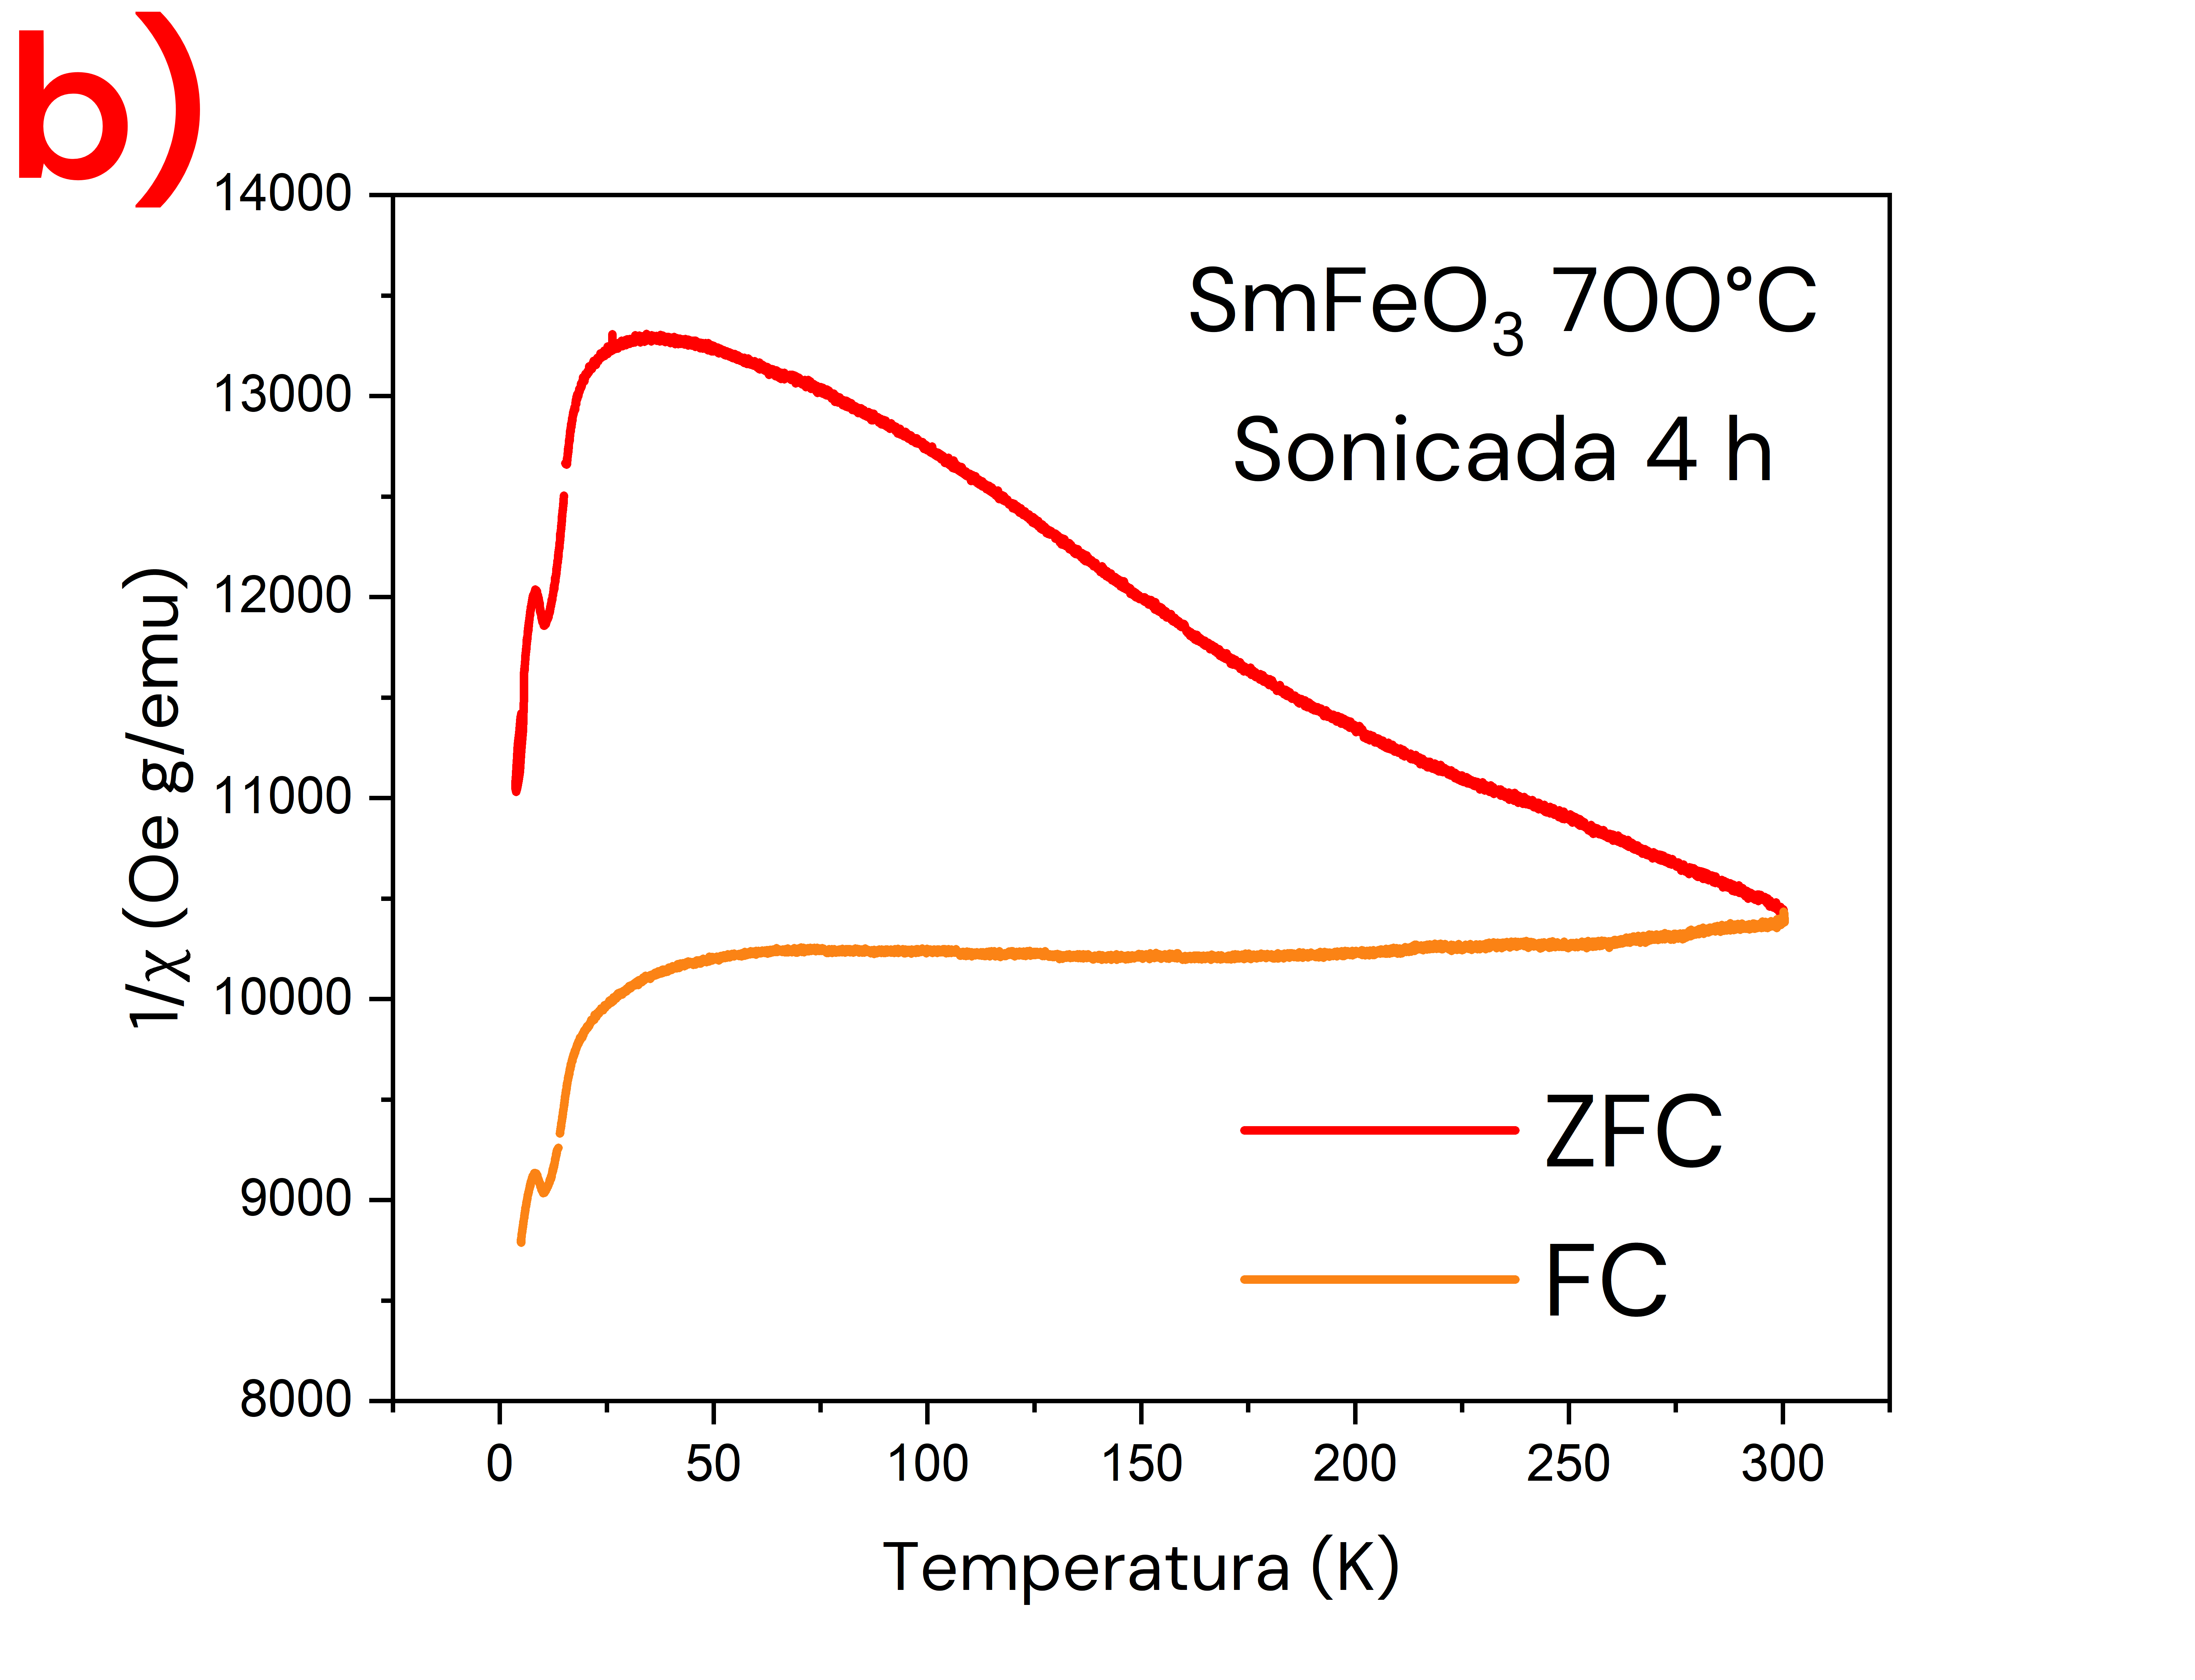
\includegraphics[width=0.45\textwidth]{fig/chivTSm-S.png}
    \includegraphics[width=0.45\textwidth]{fig/chivTSm900.png}
    \caption{Curvas $\chi$ contra $T$ para las muestras de \sama{}: a) sin sonicar y b) sonicada.}
    \label{fig:chivTSm}
\end{figure}
Las muestras de \sama{} presentan reordenamientos magnéticos a baja temperatura, teniendo un máximo local alrededor de 10 K para las muestras calcinadas a 700\gradoC{} (11.86$\pm$0.014 para la muestra sin sonicar y 10.55$\pm$0.008 para la muestra sonicada), y un mínimo local de $M$ y $\chi$ en 69.00$\pm$0.098 para la muestra calcinada a 900\gradoC{}, sin embargo este comportamiento es mucho menos pronunciado para la muestra sonicada.

En este caso, se observa una separación considerable de las curvas ZFC y FC sólo en el caso de la muestra sonicada, lo cual indica que este proceso aumentó el efecto de la anisotropía para esta muestra.
\subsubsection{Curvas de polarización}
En las figuras \ref{fig:sm100v} y \ref{fig:sm2000v} se reportan las curvas $P$ vs $E$ de las muestras de \sama{} sinterizadas.
\begin{figure}[H]
    \centering
    \includegraphics[width=0.45\textwidth]{fig/PESmFeO3100V.png}
    \quad
    \includegraphics[width=0.45\textwidth]{fig/PESmFeO3-S100V.png}
    \caption{Curvas $P$ contra $E$ (eje izquierdo) y $\chi$ contra $E$ (eje derecho) con $V_\text{max}=100$ V de las muestras de \sama{}: a) sin sonicar y b) sonicada 4 h.}
    \label{fig:sm100v}
\end{figure}
\begin{figure}[H]
    \centering
    \includegraphics[width=0.45\textwidth]{fig/PESmFeO32000V.png}
    \quad
    \includegraphics[width=0.45\textwidth]{fig/PESmFeO3-S2000V.png}
    \caption{Curvas $P$ contra $E$ (eje izquierdo) y $\chi$ contra $E$ (eje derecho) con $V_\text{max}=2000$ V de las muestras de \sama{}: a) sin sonicar y b) sonicada 4 h.}
    \label{fig:sm2000v}
\end{figure}
De forma similar a las muestras de \neod{} se observa un comportamiento de histéresis débil a $V_\text{max}=100$ V (figuras \ref{fig:sm100v} a) y b)), sin embargo, este no se pierde completamente al subir el voltaje para la muestra de \sama{} sin sonicar (figura \ref{fig:sm2000v} a)).

A continuación se reportan los valores obtenidos para $P_r$, $P_s$ y $E_c$ para las mediciones con $V_\text{max}=100$ V.

\begin{table}[H]
    \centering
    \begin{tabular}{|c||c|c|c|}
        \hline
        Muestra & $P_s$ ($\mu$C/cm$^2$) & $P_r$ ($\mu$C/cm$^2$) & $E_c$ (kV/cm) \\
        \hline\hline
        \sama{} sin sonicar & 0.0072 $\pm$ 0.00032 & $0.0022 \pm 0.00062$ & $0.3794 \pm 0.04913$ \\
        \hline
        \sama{} sonicada & 0.0054 $\pm$ 0.00018 & $0.0037 \pm 0.00011$ & $0.7354 \pm 0.05652$ \\
        \hline
        \end{tabular} 
        \caption{Valores de $P_r$, $P_s$ y $E_c$ medidos de las muestras de \sama{} sin sonicar y sonicada 4 h.}
    \label{tabla:respolarsama}
\end{table}
De igual forma se observan valores pequeños de $P_s$, $P_r$ y $E_c$ para todas las muestras. La sonicación no tuvo un efecto notorio en las propiedades eléctricas.
\end{document}